%%%%%%%%%%%%%%%%%%%%%%%%%%%%%%%%%%%%%%%%%%%%%%%%%%%%%%%%%%%%%%%
%% OXFORD THESIS TEMPLATE

% Use this template to produce a standard thesis that meets the Oxford University requirements for DPhil submission
%
% Originally by Keith A. Gillow (gillow@maths.ox.ac.uk), 1997
% Modified by Sam Evans (sam@samuelevansresearch.org), 2007
% Modified by John McManigle (john@oxfordechoes.com), 2015
% Modified by Ulrik Lyngs (ulrik.lyngs@cs.ox.ac.uk), 2018-, for use with R Markdown
%
% Ulrik Lyngs, 25 Nov 2018: Following John McManigle, broad permissions are granted to use, modify, and distribute this software
% as specified in the MIT License included in this distribution's LICENSE file.
%
% John commented this file extensively, so read through to see how to use the various options.  Remember that in LaTeX,
% any line starting with a % is NOT executed.  Several places below, you have a choice of which line to use
% out of multiple options (eg draft vs final, for PDF vs for binding, etc.)  When you pick one, add a % to the beginning of
% the lines you don't want.


%%%%% PAGE LAYOUT
% The most common choices should be below.  You can also do other things, like replacing "a4paper" with "letterpaper", etc.

% This one formats for two-sided binding (ie left and right pages have mirror margins; blank pages inserted where needed):
%\documentclass[a4paper,twoside]{templates/ociamthesis}
% This one formats for one-sided binding (ie left margin > right margin; no extra blank pages):
%\documentclass[a4paper]{ociamthesis}
% This one formats for PDF output (ie equal margins, no extra blank pages):
%\documentclass[a4paper,nobind]{templates/ociamthesis}

% As you can see from the uncommented line below, oxforddown template uses the a4paper size, 
% and passes in the binding option from the YAML header in index.Rmd:
\documentclass[letterpaper, nobind]{templates/ociamthesis}


%%%%% ADDING LATEX PACKAGES
% add hyperref package with options from YAML %
\usepackage[pdfpagelabels]{hyperref}
% change the default coloring of links to something sensible
\usepackage{xcolor}

\definecolor{mylinkcolor}{RGB}{0,0,139}
\definecolor{myurlcolor}{RGB}{0,0,139}
\definecolor{mycitecolor}{RGB}{0,33,71}

\hypersetup{
  hidelinks,
  colorlinks,
  linktocpage=true,
  linkcolor=mylinkcolor,
  urlcolor=myurlcolor,
  citecolor=mycitecolor
}



% add float package to allow manual control of figure positioning %
\usepackage{float}

% enable strikethrough
\usepackage[normalem]{ulem}

% use soul package for correction highlighting
\usepackage{color, soul}
\definecolor{correctioncolor}{HTML}{CCCCFF}
\sethlcolor{correctioncolor}
\newcommand{\ctext}[3][RGB]{%
  \begingroup
  \definecolor{hlcolor}{#1}{#2}\sethlcolor{hlcolor}%
  \hl{#3}%
  \endgroup
}
\soulregister\ref7
\soulregister\cite7
\soulregister\autocite7
\soulregister\textcite7
\soulregister\pageref7

%%%%% FIXING / ADDING THINGS THAT'S SPECIAL TO R MARKDOWN'S USE OF LATEX TEMPLATES
% pandoc puts lists in 'tightlist' command when no space between bullet points in Rmd file,
% so we add this command to the template
\providecommand{\tightlist}{%
  \setlength{\itemsep}{0pt}\setlength{\parskip}{0pt}}
 
% UL 1 Dec 2018, fix to include code in shaded environments

% User-included things with header_includes or in_header will appear here
% kableExtra packages will appear here if you use library(kableExtra)
\usepackage{booktabs}
\usepackage{longtable}
\usepackage{array}
\usepackage{multirow}
\usepackage{wrapfig}
\usepackage{float}
\usepackage{colortbl}
\usepackage{pdflscape}
\usepackage{tabu}
\usepackage{threeparttable}
\usepackage{threeparttablex}
\usepackage[normalem]{ulem}
\usepackage{makecell}
\usepackage{xcolor}


%UL set section header spacing
\usepackage{titlesec}
% 
\titlespacing\subsubsection{0pt}{24pt plus 4pt minus 2pt}{0pt plus 2pt minus 2pt}


%UL set whitespace around verbatim environments
\usepackage{etoolbox}
\makeatletter
\preto{\@verbatim}{\topsep=0pt \partopsep=0pt }
\makeatother

\counterwithout{footnote}{chapter} 

%%%%%%% PAGE HEADERS AND FOOTERS %%%%%%%%%
\usepackage{fancyhdr}
\setlength{\headheight}{15pt}
\fancyhf{} % clear the header and footers
\pagestyle{fancy}
\renewcommand{\chaptermark}[1]{\markboth{\thechapter. #1}{\thechapter. #1}}
\renewcommand{\sectionmark}[1]{\markright{\thesection. #1}} 
\renewcommand{\headrulewidth}{0pt}


% UL page number position 
\fancyhead[C]{\emph{\thepage}} %regular pages
\fancypagestyle{plain}{\fancyhf{}\fancyhead[C]{\emph{\thepage}}} %chapter pages

% JEM fix header on cleared pages for openright
\def\cleardoublepage{\clearpage\if@twoside \ifodd\c@page\else
   \hbox{}
   \fancyhead[C]{}
   \newpage
   \if@twocolumn\hbox{}\newpage
   \fi
   \fancyhead[LO]{\emph{\leftmark}} 
   \fancyhead[RE]{\emph{\rightmark}} 
   \fi\fi}


%%%%% SELECT YOUR DRAFT OPTIONS
% This adds a "DRAFT" footer to every normal page.  (The first page of each chapter is not a "normal" page.)

% IP feb 2021: option to include line numbers in PDF

% for line wrapping in code blocks
\usepackage{fvextra}
\DefineVerbatimEnvironment{Highlighting}{Verbatim}{breaklines,commandchars=\\\{\}}

% This highlights (in blue) corrections marked with (for words) \mccorrect{blah} or (for whole
% paragraphs) \begin{mccorrection} . . . \end{mccorrection}.  This can be useful for sending a PDF of
% your corrected thesis to your examiners for review.  Turn it off, and the blue disappears.
\correctionstrue


%%%%% BIBLIOGRAPHY SETUP
% Note that your bibliography will require some tweaking depending on your department, preferred format, etc.
% If you've not used LaTeX before, I recommend reading a little about biblatex/biber and getting started with it.
% If you're already a LaTeX pro and are used to natbib or something, modify as necessary.
% Either way, you'll have to choose and configure an appropriate bibliography format...


\usepackage[style=authoryear, sorting=nyt, backend=biber, maxcitenames=2, useprefix, doi=true, isbn=false, uniquename=false]{biblatex}
\newcommand*{\bibtitle}{Bibliography}

\addbibresource{bibliography/library.bib}


% This makes the bibliography left-aligned (not 'justified') and slightly smaller font.
\renewcommand*{\bibfont}{\raggedright\small}


% Uncomment this if you want equation numbers per section (2.3.12), instead of per chapter (2.18):
%\numberwithin{equation}{subsection}


%%%%% THESIS / TITLE PAGE INFORMATION
% Everybody needs to complete the following:
\title{Women prepare more than men in competitive and non-competitive environments,\\
which aligns with gender stereotypes}
\author{Keana Richards}
\college{University of Pennsylvania}

% Master's candidates who require the alternate title page (with candidate number and word count)
% must also un-comment and complete the following three lines:

% Uncomment the following line if your degree also includes exams (eg most masters):
%\renewcommand{\submittedtext}{Submitted in partial completion of the}
% Your full degree name.  (But remember that DPhils aren't "in" anything.  They're just DPhils.)
\degree{Doctor of Philosophy}
% Term and year of submission, or date if your board requires (eg most masters)
\degreedate{}

%%%%% YOUR OWN PERSONAL MACROS
% This is a good place to dump your own LaTeX macros as they come up.

% To make text superscripts shortcuts
	\renewcommand{\th}{\textsuperscript{th}} % ex: I won 4\th place
	\newcommand{\nd}{\textsuperscript{nd}}
	\renewcommand{\st}{\textsuperscript{st}}
	\newcommand{\rd}{\textsuperscript{rd}}

%%%%% THE ACTUAL DOCUMENT STARTS HERE
\begin{document}

%%%%% CHOOSE YOUR LINE SPACING HERE
% This is the official option.  Use it for your submission copy and library copy:
\setlength{\textbaselineskip}{22pt plus2pt}
% This is closer spacing (about 1.5-spaced) that you might prefer for your personal copies:
%\setlength{\textbaselineskip}{18pt plus2pt minus1pt}

% You can set the spacing here for the roman-numbered pages (acknowledgements, table of contents, etc.)
\setlength{\frontmatterbaselineskip}{17pt plus1pt minus1pt}

% UL: You can set the line and paragraph spacing here for the separate abstract page to be handed in to Examination schools
\setlength{\abstractseparatelineskip}{13pt plus1pt minus1pt}
\setlength{\abstractseparateparskip}{0pt plus 1pt}

% UL: You can set the general paragraph spacing here - I've set it to 2pt (was 0) so
% it's less claustrophobic
\setlength{\parskip}{2pt plus 1pt}

%
% Oxford University logo on title page
%
%\def\crest{{
\includegraphics[width=5cm]{templates/beltcrest.pdf}}}
%\renewcommand{\university}{University of Pennsylvania}
%\renewcommand{\submittedtext}{A thesis submitted for the degree of}
%\renewcommand{\thesistitlesize}{\fontsize{}{}\selectfont}
%\renewcommand{\gapbeforecrest}{}
%\renewcommand{\gapaftercrest}{}

% Leave this line alone; it gets things started for the real document.
\setlength{\baselineskip}{\textbaselineskip}


%%%%% CHOOSE YOUR SECTION NUMBERING DEPTH HERE
% You have two choices.  First, how far down are sections numbered?  (Below that, they're named but
% don't get numbers.)  Second, what level of section appears in the table of contents?  These don't have
% to match: you can have numbered sections that don't show up in the ToC, or unnumbered sections that
% do.  Throughout, 0 = chapter; 1 = section; 2 = subsection; 3 = subsubsection, 4 = paragraph...

% The level that gets a number:
\setcounter{secnumdepth}{2}
% The level that shows up in the ToC:
\setcounter{tocdepth}{1}


%%%%% ABSTRACT SEPARATE
% This is used to create the separate, one-page abstract that you are required to hand into the Exam
% Schools.  You can comment it out to generate a PDF for printing or whatnot.

% JEM: Pages are roman numbered from here, though page numbers are invisible until ToC.  This is in
% keeping with most typesetting conventions.
\begin{romanpages}

% Title page is created here
\thispagestyle{empty}
%%%%%%%%%%%%%%%%%%%%%%%%%%%%%%%%%%%%%%%%%%%%%%%%%%%%%%%%%%%%%%%%%%
\begin{center}
\Huge{\textbf{Title of your}} \\
\Huge{\textbf{Thesis}} \\
\vspace*{1cm}
\vspace*{1cm}
\vspace*{\fill}
\large{John Doe}\\
\end{center}



%%%%% DEDICATION -- If you'd like one, un-comment the following.
%%%%% %%%%% \begin{dedication}
%%%%%  For my mom
%%%%% \end{dedication}
%%%%% 
\phantom{\cite{?}}

%%%%% ACKNOWLEDGEMENTS -- Nothing to do here except comment out if you don't want it.

\cleardoublepage
\phantomsection
\addcontentsline{toc}{chapter}{Acknowledgements}
\renewcommand{\numberstyleacks}{plain}
\renewcommand{\numberstyleabstract}{plain}

\begin{acknowledgements}
 	This project would not have been possible without the support of many people. First, I am incredibly grateful for the support of my mom, Dawn Eden, who has been guiding me in my academic and personal pursuits my whole life. She has sacrificed her own sleep, money, and time on endless occasions to help me get to this point, with an optimism that still inspires and motivates me. I have learned and continue to learn so much from her. I would also like to thank many of my other family members whose support made this dissertation possible. I am especially grateful to my brother, Jared Richards, for being my partner in crime on occasions that would have otherwise been boring and for teaching me so much about spaces that I know very little about.

  Many thanks to my advisers, Coren Apicella and Emily Falk, for their invaluable advice, continuous support, and patience during my PhD journey. I am also grateful for my committee members, Geoffrey Goodwin and Gideon Nave, who offered substantial guidance and support over the last few years of the PhD.

  Finally, I would not have been able to finish the thesis if it were not for the numerous friends that have been sources of support, conversation, and laughter during my writing journey. Having enjoyable conversations and experiences to look forward to after writing at the end of the day motivated me to continue working on this project, especially on days where thinking about the thesis was the last thing I wanted to do.
\end{acknowledgements}



%%%%% ABSTRACT -- Nothing to do here except comment out if you don't want it.

\addcontentsline{toc}{chapter}{Abstract}
\renewcommand{\numberstyleabstract}{plain}

\renewcommand{\abstracttitle}{Abstract}
\begin{abstract}
	Gender gaps in economic outcomes persist, despite women's gains in education. Various explanations have been proposed for these persistent gaps, including gender differences in competitiveness. In both lab and field studies, women tend to compete less than men, despite performing just as well. Across three studies in Chapter 1 involving over 3000 participants recruited from Amazon Mechanical Turk, we experimentally test whether variations of preparation (i.e., knowledge of an opportunity to prepare, limited opportunity to prepare, and unlimited opportunity to prepare) before performance reduce gender differences in willingness to compete. We also measure participants' choice to prepare and elicit their beliefs about whether men or women will prepare more. First, we show that the preparation intervention does not increase women's competitiveness across studies. Instead, we discover a novel gender difference in the choice to prepare before performance regardless of one's competitiveness, risk aversion, and confidence.\\
 \newpage

 This finding aligns with participants' incentivized beliefs - the majority of participants correctly predicted that women would practice more than men. Given this novel finding, Chapter 2 experimentally tests whether the gender difference in preparation may be exacerbated in competitive environments relative to non-competitive environments (N = 3980). Although we replicate the gender difference in preparation, we find no evidence that competitions increase preparation in men or women. This means that women prepare more than men regardless of whether they were assigned to compete. Again, this aligns with participants' incentivized beliefs about gender differences in preparation. This dissertation discusses the downstream and potentially negative consequences of interventions designed to get women to compete, such as the one introduced here. It also discusses both the causes and implications of this newly discovered gender difference in preparation. Future research should explore the boundary conditions, moderators, and mediators of the newly discovered gender difference in preparation. Finally, rather than designing interventions that encourage women to compete more, we implore future research to focus on exploring interventions that change the system to be more gender-inclusive.
\end{abstract}



%%%%% MINI TABLES
% This lays the groundwork for per-chapter, mini tables of contents.  Comment the following line
% (and remove \minitoc from the chapter files) if you don't want this.  Un-comment either of the
% next two lines if you want a per-chapter list of figures or tables.
  \dominitoc % include a mini table of contents

% This aligns the bottom of the text of each page.  It generally makes things look better.
\flushbottom

% This is where the whole-document ToC appears:
\tableofcontents

% Uncomment to generate a list of tables:
\listoftables
  \mtcaddchapter


\listoffigures
	\mtcaddchapter
  	% \mtcaddchapter is needed when adding a non-chapter (but chapter-like) entity to avoid confusing minitoc

%%%%% LIST OF ABBREVIATIONS
% This example includes a list of abbreviations.  Look at text/abbreviations.tex to see how that file is
% formatted.  The template can handle any kind of list though, so this might be a good place for a
% glossary, etc.

% The Roman pages, like the Roman Empire, must come to its inevitable close.
\end{romanpages}

%%%%% CHAPTERS
% Add or remove any chapters you'd like here, by file name (excluding '.tex'):
\flushbottom

% all your chapters and appendices will appear here
\hypertarget{chapter-1-introduction}{%
\chapter{Chapter 1: Introduction}\label{chapter-1-introduction}}

\adjustmtc
\markboth{Introduction}{}

Women's labor force participation has increased exponentially over the past several decades \autocite{Goldin2006a,Statistics2020}, rising from 32\% to 57\% between 1960 and 2018 (where women here are defined as 16 years or older) \autocite{Statistics2020,Blau2017,Eagly2019}, while men's participation has decreased over the same period (from 82\% to 69\%). As a result, the gender gap in labor force participation fell to a 12\% difference. Additionally, women have been increasingly entering previously male-dominated occupations \autocite{Blau2013,Reskin2009,England2010}.

Despite progress towards gender equality (e.g., women's suffrage, a reversal of the gender education gap, women's increased participation in the labor market) \autocite{Goldin2014,Goldin2006a,Goldin2006,Blau2010,Blau2013,Blau2014,Bianchi2012,Sayer2005}, gender gaps in the labor market persist \autocite{Blau2017,Goldin2014,Hegewisch2014,Bertrand2001,Blau2014,Levanon2016,Blau2006b,Blau2006a}. One of the most highly cited and tangible metrics for gender disparities in the labor market is the gender wage gap \autocite{Blau2000,Blau2017,Nyhus2012,McGee2015,Goldin2014,Hegewisch2014,Bertrand2001,Blau2006b}. Recent unadjusted estimates suggest women earn only 79.3\% of what men earn \autocite{Blau2017}.

In the past, gender gaps in education and full-time labor market experience explained a large proportion of the gender wage gap (i.e., 27\% in 1980) \autocite{Blau2017}. As women's education and labor force experience has increased over time \autocite{Goldin2006a}, the impact of these variables on the gender wage gap has decreased (e.g., 8\% in 2010) \autocite{Blau2017}. Since there has been a slowing convergence of the wage gap in recent years \autocite{Blau2006b}, identifying and understanding the factors that perpetuate gender differences in labor market outcomes, such as the persistent gender wage gap, is crucial for achieving gender equality in the long-term.

One area that has been explored extensively within the economics literature is gender differences in competitiveness, both in terms of the choice to compete \autocites[for review, see][]{Niederle2011,Niederle2017a}, to a lesser extent, response to competitions (e.g., performance during competition) \autocite{Gneezy2003,Gneezy2004,Gunther2010,Samak2013}. These studies typically find that women choose to compete less than men, and that they tend to respond less to competition (that is, their performance does not significantly increase to the extent that men's performance does in competitive contexts). Research suggests these gender differences in competitiveness may have implications for real-world economic outcomes \autocite{Buser2014,Zhang2012,Buser2017c,Buser2017b,Samek2019,Berge2015,Reuben2015,Reuben2017}. For instance, \textcite{Buser2014} show that the typical measure of competitiveness used in the lab explains about 20\% of gender differences in the choice in an academic track for students entering high school. On the other hand, \textcite{Reuben2015} show that gender differences in competitiveness explain about 10\% of gender differences in earnings among MBA graduates. Considering these findings, researchers began exploring interventions to increase competitiveness, including enacting gender quotas \autocite{Niederle2013,Sutter2016}, replacing other-competition (i.e., competing against performance of other individuals) with self-competition (i.e., competing against one's previous performance) \autocite{Bonte2018,Carpenter2018,Klinowski2019,Apicella2017a,Apicella2020}, and relaxing pressure during competitions \autocite{Shurchkov2012}, among many others \autocite[see][ for a review]{Niederle2017a}. We expected that preparation may serve as a viable intervention for increasing women's competitiveness (i.e., choice to compete), since preparation may increase confidence in one's performance and/or reduce perceptions of risk of competition entry, factors that have been well-established as contributors to the gender gap in competitiveness \autocite{Niederle2011}, if not factors that fully explain the gender gap \autocite{Veldhuizen2017,Gillen2019}.

Thus, it is possible that giving people the chance to prepare would reduce gender disparities in competition. On the other hand, opportunities to prepare might also result in opportunity costs for women, such that women might end up preparing more than necessary before performing. Since prior interventions have not tested the effects of offering individuals the opportunity to prepare before entering a competition, we address this gap in the literature on gender differences in competitiveness through a series of experiments in Chapter 1 where we offer participants variations of the opportunity to prepare (i.e., knowledge of preparation, limited opportunity to prepare, and unlimited opportunity to prepare). We test whether the gender gap in competitiveness is eliminated in the preparation conditions relative to the control conditions. Our research in Chapter 1 also had the explicit goal of identifying whether there are any gender differences in preparation, since any observed gender differences in the tendency to (over)prepare could create opportunity costs for those who choose to prepare. Given the well-established gender differences in risk attitudes and confidence, we reasoned that they might contribute to differences in the desire to prepare before performance. Results from Chapter 1 showed that there are in fact gender differences in preparation, though we did not find gender differences in competitiveness after controlling for gender differences in risk attitudes and confidence. Given these intriguing and novel results, the experiment in Chapter 2 tests whether the gender difference in preparation would be exacerbated in competitive settings, such that women would be especially likely to prepare before entering a competitive, relative to non-competitive, setting. Chapter 2 also seeks to understand the gender difference in preparation further by exploring whether women are more likely to perceive that they prepare less than others relative to men, especially in competitive settings. Overall, these findings have implications for the literature on gender differences in competitiveness and also contribute more generally to our understanding of how interventions intended to reduce gender differences may have negative downstream consequences (e.g., potential opportunity costs of (over)preparing). In addition, we discover a novel gender difference in preparation, which we encourage future research to explore further.

\hypertarget{chapter-2-effects-of-preparation-on-gender-differences-in-willingness-to-compete}{%
\chapter{Chapter 2: Effects of preparation on gender differences in willingness to compete}\label{chapter-2-effects-of-preparation-on-gender-differences-in-willingness-to-compete}}

\hypertarget{introduction}{%
\section{Introduction}\label{introduction}}

\hypertarget{gender-gaps-persist-despite-womens-success-in-education}{%
\subsection{Gender gaps persist despite women's success in education}\label{gender-gaps-persist-despite-womens-success-in-education}}

Women have surpassed men in education outcomes, like college attendance and graduation rates \autocite{Blau2017,Goldin2006,Stoet2015}, but continue to be underrepresented in top management positions in nearly all sectors \autocite{Bertrand2001}. And, a sizable gender wage gap still persists \autocite{Blau2017}. Traditional economic variables, such as household division of labor and discrimination, account for some, but not all, of these disparities \autocite{Blau2017}. As such, researchers have begun to consider psychological gender differences, including the predilection for competition, as means of understanding persistent gender gaps in labor market outcomes \autocite[for review, see][]{Niederle2011}. Specifically, they expected that gender differences in competitiveness may explain why women may not compete for promotions and are underrepresented in top-level or highly competitive positions (e.g., CEO) \autocite{Niederle2007}.

\hypertarget{gender-differences-in-competitiveness}{%
\subsection{Gender differences in competitiveness}\label{gender-differences-in-competitiveness}}

Research suggests women are, on average, less competitive than men \autocites[for review, see][]{Niederle2011,Croson2009,Niederle2017b,Shurchkov2018}, conditional on ability and other factors relevant to competitiveness. Foundational work on gender differences in competitiveness operationalized competitiveness as the choice of a tournament payment scheme, that reaps potentially higher earnings but requires outperforming an opponent, over a piece-rate scheme, where participants are paid per unit of work they produce \autocites{Niederle2007}[although see][ for an arguably more sensitive test of gender differences in competitiveness]{Saccardo2018}. In this paradigm, women are less likely to enter tournaments while completing mathematical problems, even when they would have earned more by competing \autocite{Niederle2007}. Numerous conceptual replications over the past 15 years suggest that the gender difference in willingness to compete is robust \autocites[see][ for review]{Niederle2011,Niederle2017a,Niederle2017b}. Notably, this effect has been replicated in diverse populations (e.g., across age groups and cultures) \autocite{Apicella2015,Buser2014,Sutter2016,Andersen2013,Buser2017b,Sutter2010,Dreber2014,Mayr2012} and with a diverse set of tasks \autocite{Apicella2015,Saccardo2018,Bjorvatn2016,Sutter2015,Frick2011,Samek2019}. However, there is evidence that the task used during competition affects the size of the gender gap. For instance, some research suggests that when the task is female-typed or gender-neutral, the gender gap in willingness to compete may be reduced or eliminated \autocite{Iriberri2017,Boschini2014,Boschini2019,Apicella2015,Grosse2010,Gunther2010,Dreber2014,Dreber2011,Shurchkov2012}. Drawing from the psychology literature on stereotype threat \autocite{Steele1997,Spencer1999,Spencer2016}, negative stereotypes about women's ability to perform male-typed tasks (e.g., math, mental rotation) may produce anxiety and undermine performance. As a result, women may decide not to engage in a competition because they either believe the stereotype or because the stereotype provokes enough anxiety to reduce performance \autocite{Gunther2010,Grosse2010,Iriberri2017,Shurchkov2012}.

Importantly, this laboratory measure of competitiveness based on the preference between a tournament and piece-rate payment scheme predicts labor market outcomes, including education choices \autocite{Buser2014,Zhang2012,Buser2017c,Buser2017b}, entrepreneurial decisions (e.g., investment, employment) \autocite{Berge2015}, and both expected and actual earnings \autocite{Reuben2015,Reuben2017}. Thus, understanding why men and women differ in levels of competitiveness and whether interventions exist that can reduce or eliminate the difference may be key for solving the pernicious gender gaps in the labor market. In fact, many of the most crucial time points during one's career that determine later success (e.g., job interviews, university and post-baccalaureate entrance exams, promotion) require competing against others for a limited number of slots and substantially higher earnings.

\hypertarget{risk-attitude-and-confidence-as-proposed-mechanisms-for-gender-difference-in-competitiveness}{%
\subsection{Risk attitude and confidence as proposed mechanisms for gender difference in competitiveness}\label{risk-attitude-and-confidence-as-proposed-mechanisms-for-gender-difference-in-competitiveness}}

Both confidence and risk attitudes have been implicated in driving gender differences in willingness to compete \autocite{Niederle2011,Veldhuizen2017}. However, the extent to which confidence and risk attitudes account for the gender difference in willingness to compete is debated. The foundational research in this literature suggests that confidence and risk attitudes do not completely explain gender differences in competitiveness, since a residual gap remained after controlling for these factors \autocite{Niederle2007}. As a result, the unexplained component of the original gender effect was taken as evidence of a distinct ``competitiveness'' trait, separate from risk attitudes and confidence \autocite{Niederle2007,Niederle2011}. Conversely, recent work correcting for measurement error \autocite{Gillen2019} and using experimental techniques to isolate the effects of the competitiveness trait \autocite{Veldhuizen2017} suggests that risk attitudes and confidence can fully explain the gender gap in the choice to compete.

Regardless of whether competitiveness is a ``stand-alone'' trait, it is clear that both confidence and risk attitudes influence how men and women react to competitions. For instance, even in the original study by \textcite{Niederle2007}, 27\% of the gender gap in tournament entry was explained by men being more overconfident than women about their relative performance on the task. As such, interventions designed to correct men's overconfidence, increase women's confidence, or decrease women's perceptions of risk and uncertainty in competitive contexts may help reduce the gender gap in competitiveness.

\hypertarget{gender-differences-in-confidence}{%
\subsubsection{Gender differences in confidence}\label{gender-differences-in-confidence}}

Within the literature on the gender gap in competitiveness, confidence is operationalized as the belief about one's relative performance during a competition, where individuals who have inaccurately high (low) ratings of their performance are deemed overconfident (underconfident) \autocites{Niederle2011}[also see overplacement in][]{Moore2008,Moore2017}. If an individual does not believe their performance is higher than the individuals they are competing against, they are unlikely to make the decision to compete for fear of losing.

While most individuals are overconfident \autocite{Alicke2013,Dunning2004b}, there is ample research to suggest that women are less (over)confident on average than men across a number of domains \autocites{Mobius2011,Niederle2011,Croson2009,Lundeberg1994,Niederle2007,Bertrand2010a,Beyer1990,Beyer1997,Jakobsson2013}[although see][]{Bandiera2022}. Because women are less overconfident, they compete less often than they should, given their actual ability \autocite{Niederle2007}. Confidence too may help explain why, in some situations, the gender gap in competitiveness may be reduced or eliminated. For instance, women tend to compete more when tasks are female-typed or gender-neutral \autocite{Iriberri2017,Boschini2014,Boschini2019,Apicella2015,Grosse2010,Gunther2010,Dreber2014,Dreber2011,Shurchkov2012}, when they are facing other women \autocite{DattaGupta2013,Booth2012}, or when competing against themselves \autocite{Apicella2017a,Bonte2018,Carpenter2018,Apicella2020}. For example, \textcite{Apicella2017a} document a gender difference in confidence when women and men are competing against other individuals, but not when they are competing against themselves (i.e., their own past performance). There are several non-mutually exclusive and potentially interacting explanations that could account for women's relatively lower (over)confidence, including differences in performance or ability, experience, innate psychological differences, and stereotype threat \autocite{Steele1997,Spencer1999,Spencer2016}. In the latter case, for instance, women may decide to forgo competitions because they either believe negative stereotypes about their ability to perform certain tasks, or because stereotypes provoke enough anxiety to reduce confidence \autocite{Gunther2010,Grosse2010,Iriberri2017,Shurchkov2012,Burow2017}. Taken together, this body of research suggests that interventions designed to increase confidence in women may embolden them to compete more.

\hypertarget{gender-differences-in-risk-attitude}{%
\subsubsection{Gender differences in risk attitude}\label{gender-differences-in-risk-attitude}}

A second variable that has been identified as a possible explanation for gender differences in competitiveness is risk attitudes, typically construed as the preference for a certain gain over a gamble, even if the gamble has an equal or greater monetary expectation \autocite{Kahneman1982}. Researchers investigating gender differences in risk attitudes find that men are typically more risk-seeking than women \autocite{Eckel2008,Charness2012,Croson2009,Bertrand2010a}, including in hunter-gatherers \autocite{Apicella2017}, but see \autocite{Harrison2007} for an exception. While most studies report a gender difference, the difference appears to be small to medium \autocite{Filippin2016} and culturally-dependent \autocite{Gneezy2009}.

Competitive payment schemes are inherently riskier than piece-rate payment schemes because the variance in returns is greater. With piece-rate payment schemes, individuals are guaranteed a certain amount for every unit they produce. Moreover, there typically exists uncertainty in competitions since one's relative performance is unknown \autocite{Niederle2011}. Indeed, some of the gender gap in competitiveness is explained by men and women's differing risk attitudes \autocite{Niederle2011}. In fact, some recent work suggests that nearly 30\% of the gender gap in competitive choices can be explained by risk attitudes \autocite{Gillen2019,Veldhuizen2017}.

\hypertarget{why-preparation-may-eliminate-gender-gap-in-competitiveness-by-changing-confidence-andor-risk-attitude}{%
\subsection{Why preparation may eliminate gender gap in competitiveness by changing confidence and/or risk attitude}\label{why-preparation-may-eliminate-gender-gap-in-competitiveness-by-changing-confidence-andor-risk-attitude}}

Preparation or training on a task may increase one's confidence \autocite{Gist1992,Schunk1981,Schunk1982,Usher2008}, since people usually are able to observe an improvement in their performance over time. In fact, there is evidence that preparation (as measured through studying) does causally affect academic performance among university students \autocite{Stinebrickner2008}. In line with increased confidence after preparation or training, \textcite{Lent1996} found that college students listed past accomplishments as the most influential factor in determining their confidence. Moreover, research directly comparing the effects of mastery experiences (via preparation), vicarious experiences (e.g., watching others perform a task), and a control treatment without any intervention on confidence found that mastery increased confidence significantly more than vicarious experiences and the control treatment \autocite{Bandura1977a}. Other research suggests that women are less likely to be confident in their answers when asked about topics outside of their field of expertise, leading to a confidence gap \autocite{Sarsons2021}. This suggests that gaining expertise, perhaps through practicing, may selectively boost women's confidence. \textcite{Roll2011} found that practicing mathematics problems, using an intelligent tutoring system, significantly decreases underconfidence but has no effect on rates of overconfidence. This too suggests that practicing may preferentially benefit women who are more likely than men to be underconfident. That said, if practicing only helps with underconfidence, when most people, including women, are overconfident, then its application may be limited.

Preparation, and the feelings of preparedness or self-efficacy that follow, may also decrease the perceived riskiness of competitions. With increased self-efficacy, individuals may believe their probability of winning in a competition is higher than those with lower self-efficacy. Surprisingly little work has explored how preparation impacts men's and women's risk attitudes. However, some experimental work suggests that manipulating perceived competence on a task by giving participants positive feedback about their performance on a task can lead to significantly more risk-taking behavior \autocite{Krueger1994}. The researchers were able to rule out the role of mood in driving the results by giving some participants positive feedback on one task and negative feedback on another. For these participants, risk-taking increased in the positive feedback condition and decreased in the negative feedback condition. Interestingly, \textcite{Gysler2002} find that knowledge -- in this case, understanding of financial markets -- and confidence in that knowledge, negatively correlate with women's risk aversion, but positively correlate with men's risk aversion. This suggests that preparation may disproportionately increase risk-taking in women. Finally, there is evidence that risk attitudes play a greater role in predicting decisions to compete when individuals are competing against other individuals, rather than themselves (i.e., their own past performance), possibly because there is more uncertainty in estimating an opponent's ability versus one's own ability \autocite{Apicella2017a}.

\hypertarget{previous-literature-looking-at-preparation-on-competition-entry}{%
\subsection{Previous literature looking at preparation on competition entry}\label{previous-literature-looking-at-preparation-on-competition-entry}}

Surprisingly, little work has explored how preparation impacts men and women's confidence, risk attitudes, or their willingness to compete. We know of only one study that has explored how delaying a competition, and in some cases, offering an opportunity to study, affects decisions to compete. In a working paper, \textcite{Charness2021} examine whether gender gap entry rates change when a future opportunity to study for the task is made available. The authors hypothesized that women would be more likely to compete when there is an opportunity to study for the task. Contrary to their prediction, the authors found that providing an option to study leads men to be more likely to enter into future planned tournaments and leads women to be less likely to enter into these tournaments, resulting in a significant gender gap. However, this gap was only present during the initial, provisional sign-up period. When the actual choice was made later -- sometime between one and five days -- the gender difference disappeared. Of those men who returned to complete the study, some switched into the non-competitive payment scheme. The authors suggest that the results may be explained by men being overly confident in their future selves' resolve to study.

\hypertarget{the-current-experiments}{%
\subsection{The current experiments}\label{the-current-experiments}}

We examine the role of preparation on the gender differences in willingness to compete through three experiments. However, unlike \textcite{Charness2021}, we do not introduce a significant time delay in our studies. That is, experiments took place in a single session, thus minimizing any potential for gender differences in beliefs about future behavior to affect our results.

In the first experiment, we test whether simply knowing that there will be an opportunity to prepare before performing a task affects the gender gap in willingness to compete. That is, we manipulate participants' knowledge of whether they will have time to prepare before they make their decision to compete. We anticipated that participants with this information would be more inclined to compete compared to participants without this information and that this effect would be stronger for women. Thus, we expected a main effect of condition and an interaction between gender and condition on the choice to compete. In the second experiment, we examined how actual preparation influences the decision to compete. That is, we manipulated whether participants were required to prepare before making the decision to compete. Again, we expected that women in the preparation condition would be more inclined to compete than women in the no preparation condition, while we did not expect men's competitiveness to be significantly affected by the preparation manipulation.

Finally, in experiment 3, we examine how an unlimited amount of preparation affects gender differences in the willingness to compete. Across all experiments, we measured gender differences in actual preparation after administering the treatment and eliciting preferences to compete. Finally, we monetarily incentivized participants in both studies to correctly predict whether men or women would prepare and compete more. The research design, pre-registered hypotheses, measures and analyses are available on \href{https://osf.io/q39a5/}{OSF} and all analyses were conducted in R statistical software (version 4.0.4). All participants across the three experiments were recruited through Amazon Mechanical Turk (or MTurk), with a guaranteed payment and the opportunity to earn bonuses depending on their performance and the performance of others. Recruiting participants on this platform allowed for efficient data collection while meeting acceptable psychometric standards, such as high test-retest and alpha reliability \autocite{Rand2012,Buhrmester2011,Paolacci2014,Chandler2016}.

\newpage

\hypertarget{study-1}{%
\section{Study 1}\label{study-1}}

\hypertarget{methods}{%
\subsection{Methods}\label{methods}}

\hypertarget{participants}{%
\subsubsection{Participants}\label{participants}}

All study measures described below are publicly available on OSF both as a \href{https://osf.io/hb9nw/}{.pdf} and \href{https://osf.io/ga24t/}{.qsf}. Participants on Amazon Mechanical Turk who opted into the study had to pass several screening questions. Specifically, participants included in the paid portion of the study had to (i) identify their nationality as American and live in the United States, (ii) identify as a man or a woman, and (iii) be using a computer (rather than a phone or tablet). If they did not meet these criteria, they did not proceed to the paid portion of the study. Additionally, upon reviewing the data, we had reason to suspect that some participants completed the study more than once. Specifically, some participants had the same IP address, MTurk ID, and were of the same gender. When entries matched on all three identifiers, we included only the first entry and excluded all subsequent entries. The final sample consisted of 1056 participants (53.6\% women), with an average age of 37.74 (\emph{SD} = 13.19) years.\footnote{Note: Per our screening criteria for participants, the number of participants who do not identify as men or women is 0 across all studies. Therefore, the proportion of men in the sample is represented by whatever proportion of the full sample does not identify as women} 54 participants (53.7\% women) dropped out of the study before finishing and we use their data when available. See Table \ref{tab:demographics-table-study1} for all demographic information.

\newpage

\begin{center}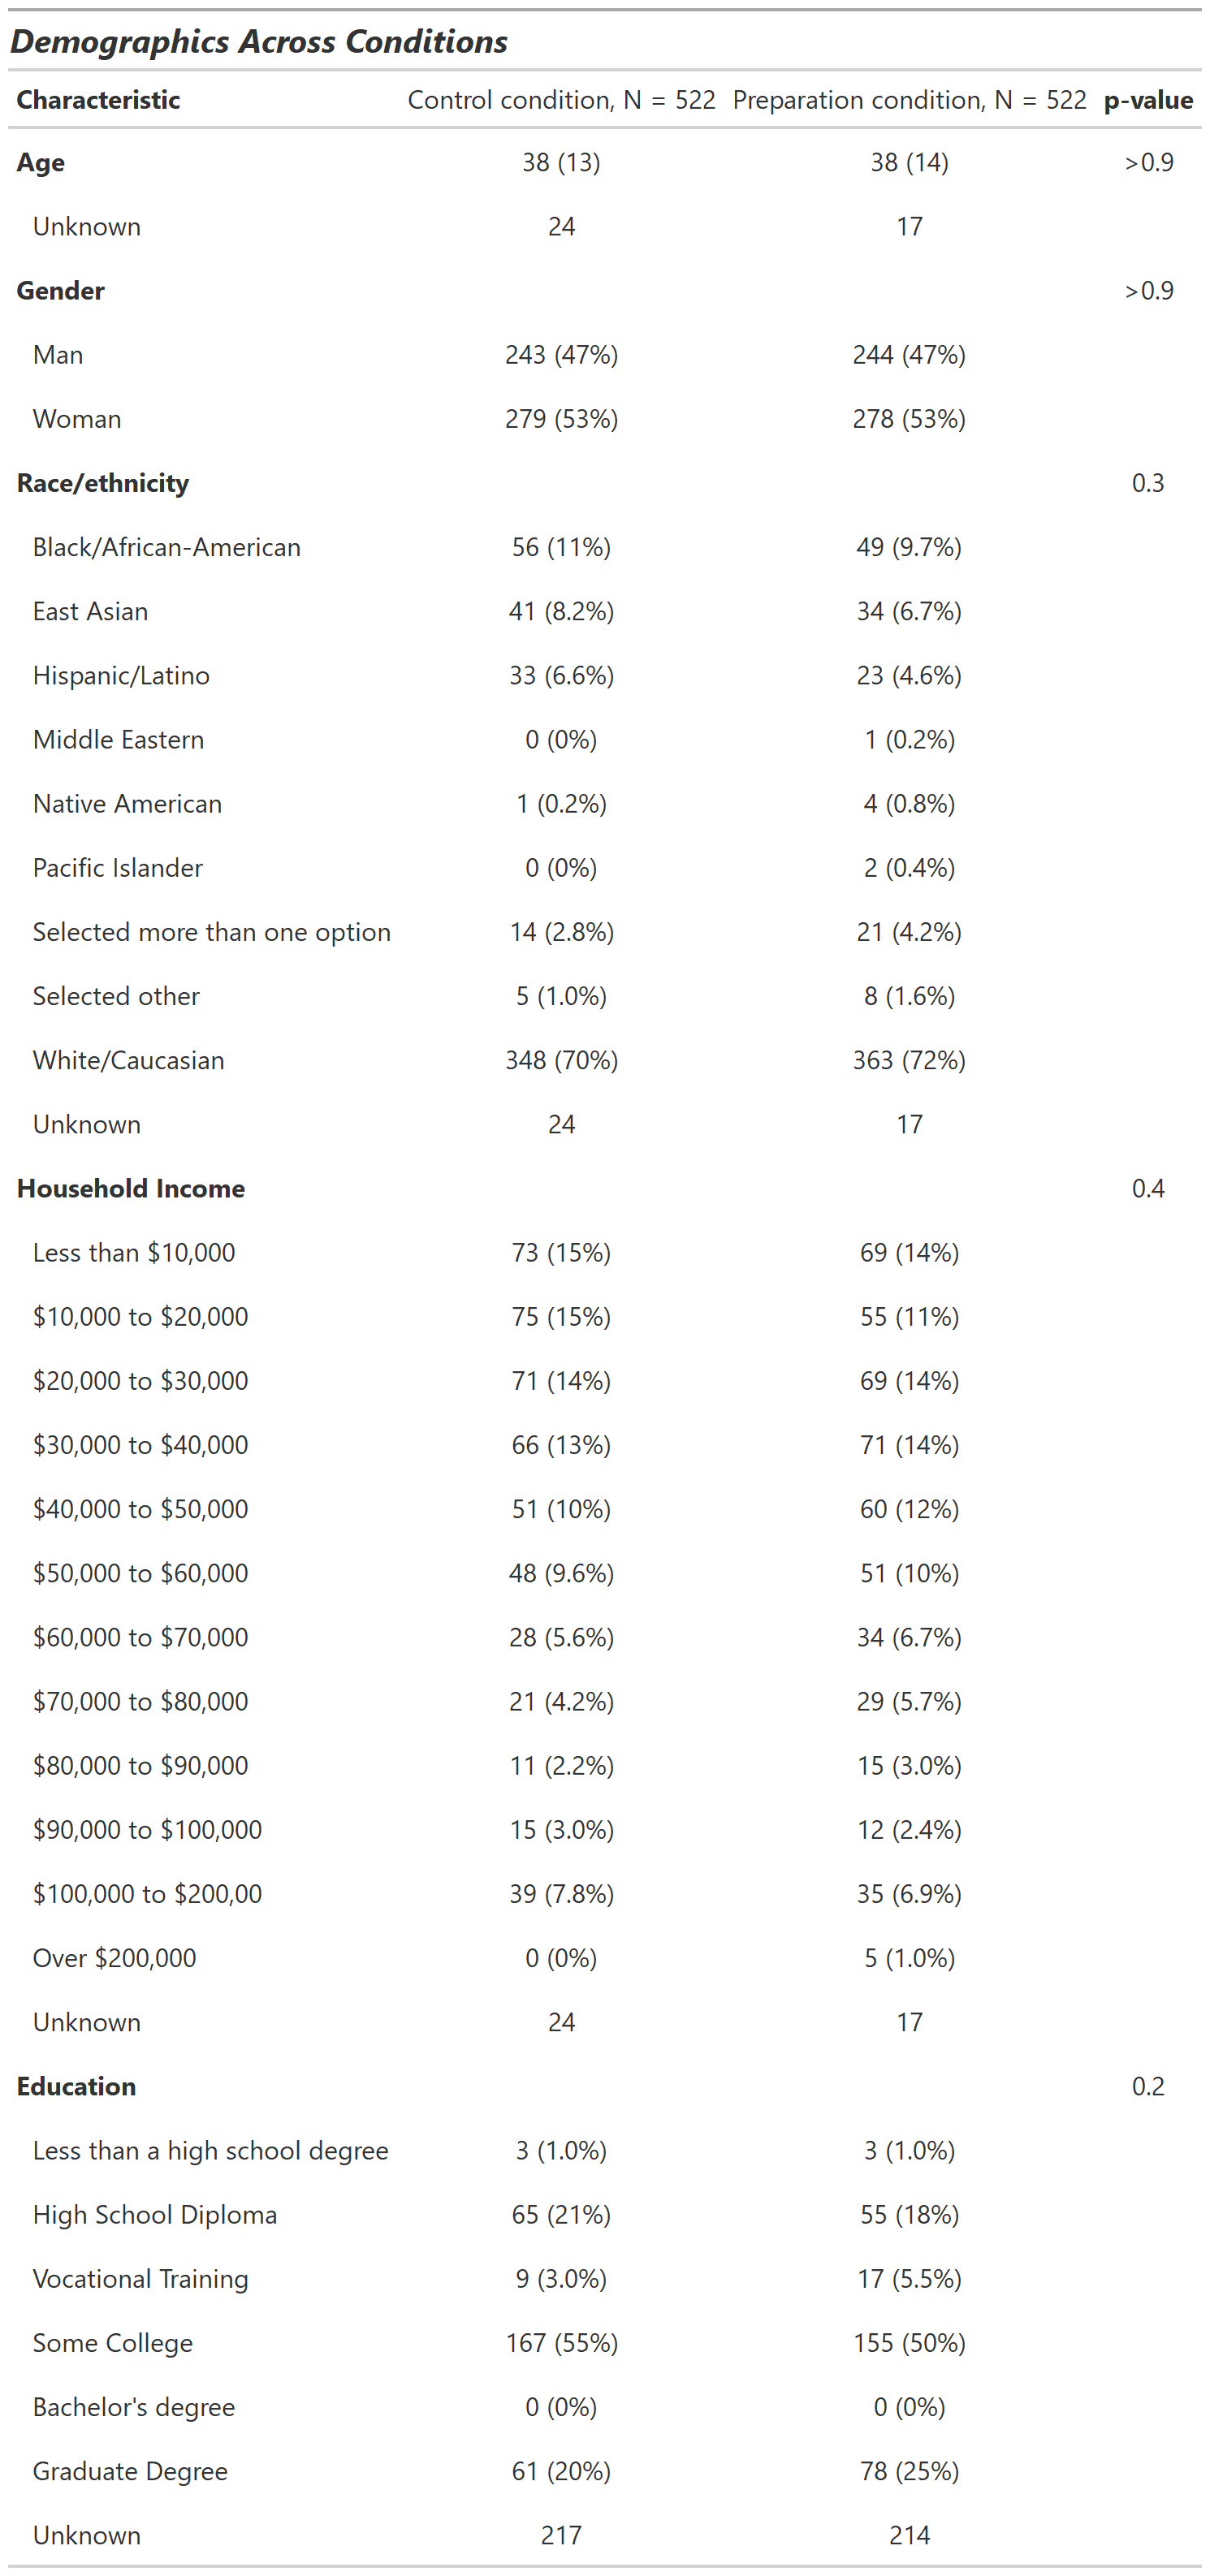
\includegraphics[width=0.6\linewidth]{C:/Users/keana/OneDrive - PennO365/Comp_transfer2018/Penn/practice_study/gender-practice/study1/figs/demographics-table-conds-study1} \end{center}

\begin{table}[ht]
\centering
\begingroup\fontsize{0.1pt}{0.1pt}\selectfont
\begin{tabular}{r}
   \\ 
 \end{tabular}
\endgroup
\caption{Size of sample in Study 1 with corresponding percentage listed for gender, race, education, and household income, with p-values derived from Fisher’s exact test. Mean with corresponding standard deviation listed for age, with p-values derived from Kruskal-Wallis test. If a participant did not respond to a given question, we list their response as ‘Unknown’.} 
\label{tab:demographics-table-study1}
\end{table}

\newpage

\begin{center}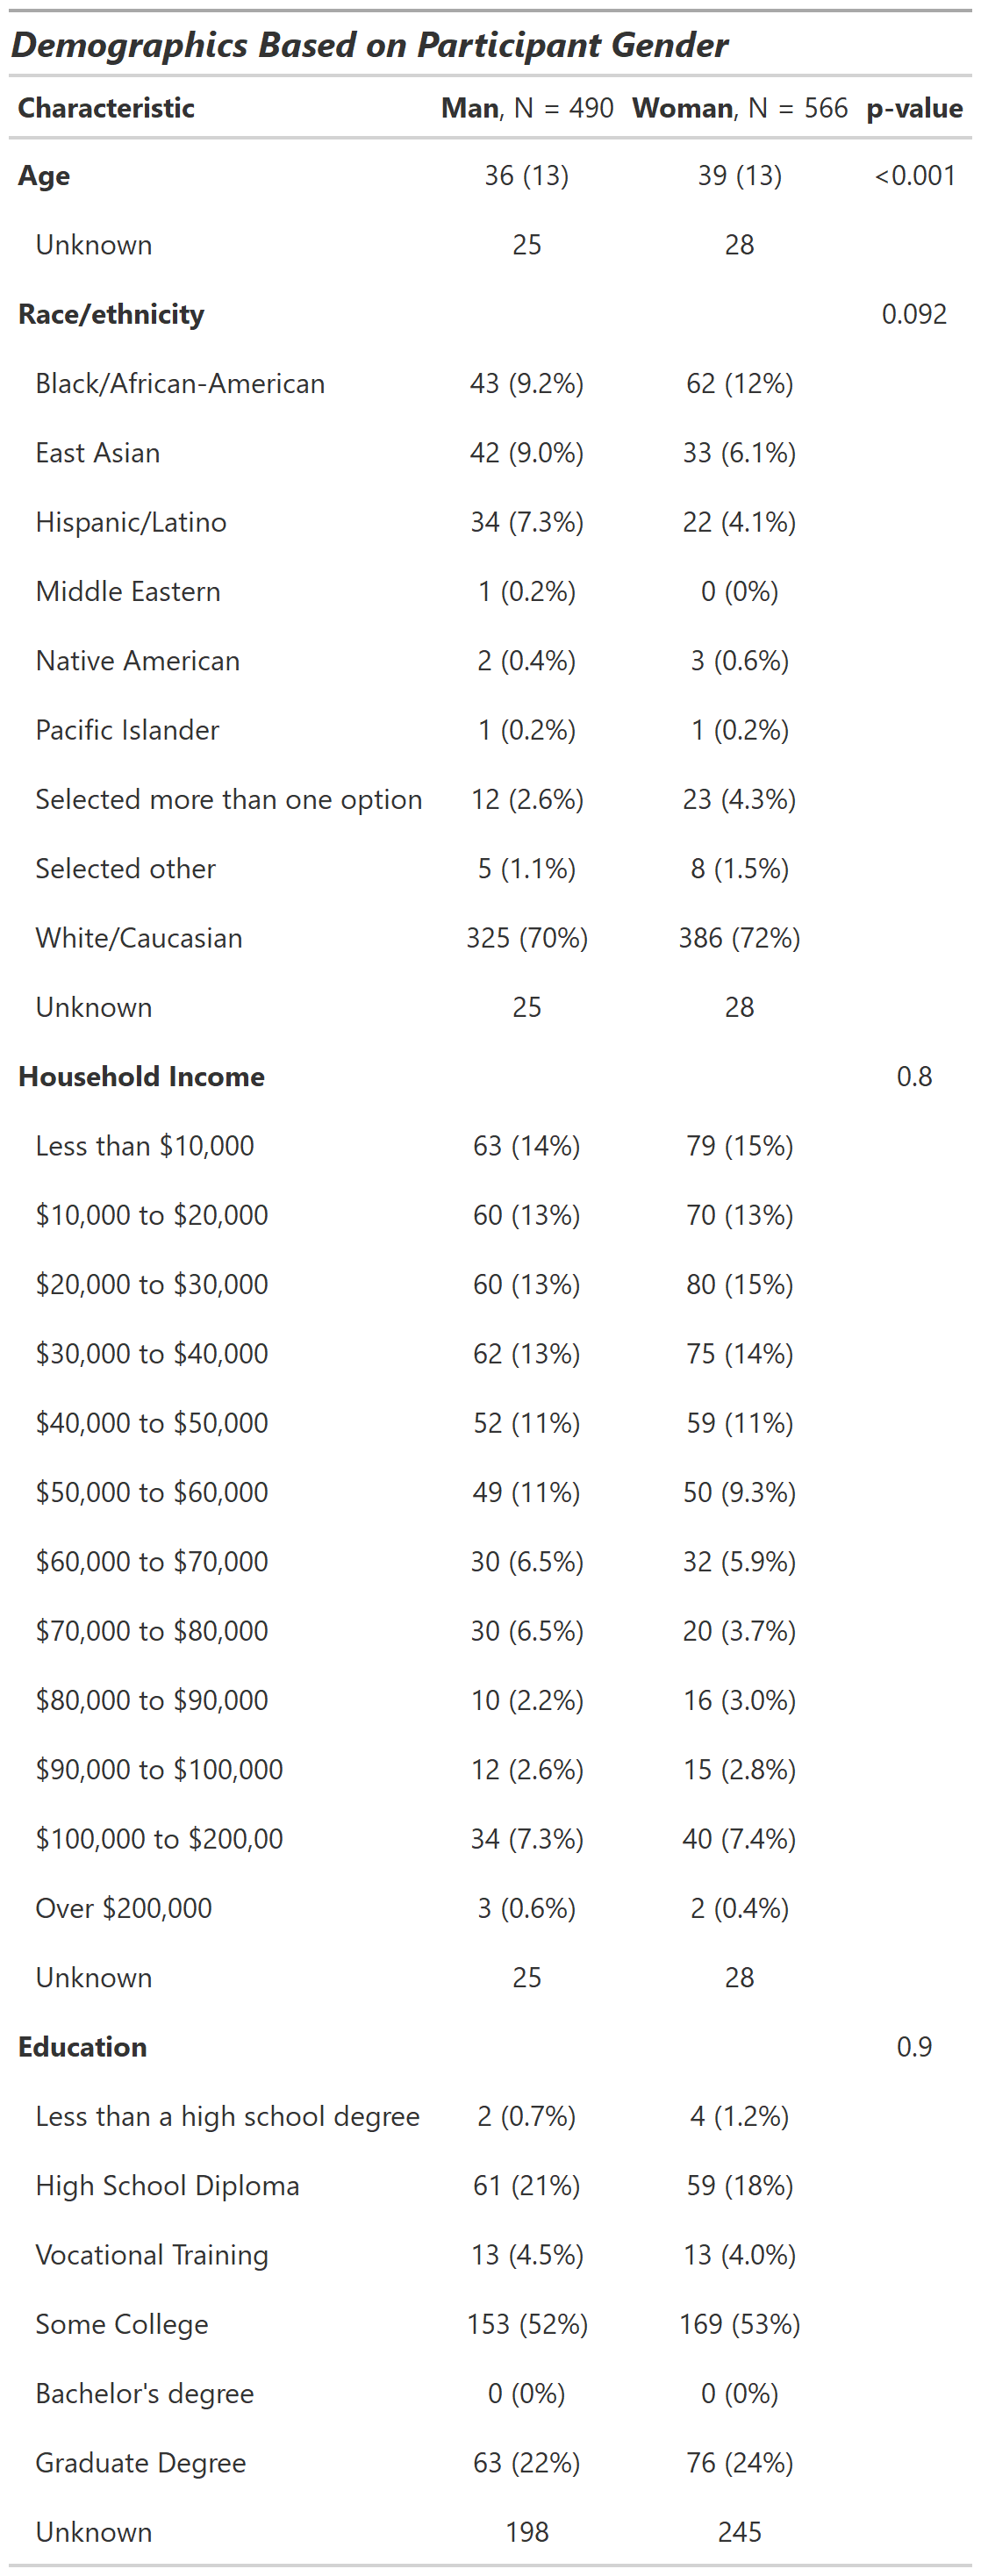
\includegraphics[width=0.5\linewidth]{C:/Users/keana/OneDrive - PennO365/Comp_transfer2018/Penn/practice_study/gender-practice/study1/figs/demographics-table-gender-study1} \end{center}

\begin{table}[ht]
\centering
\begingroup\fontsize{0.1pt}{0.1pt}\selectfont
\begin{tabular}{r}
   \\ 
 \end{tabular}
\endgroup
\caption{Size of sample in Study 1 with corresponding percentage listed for race, education, and household income, with p-values derived from Fisher’s exact test. Mean with corresponding standard deviation listed for age, with p-values derived from Kruskal-Wallis test. If a participant did not respond to a given question, we list their response as ‘Unknown’.} 
\label{tab:demographics-table-gender-study1}
\end{table}

\hypertarget{procedures}{%
\subsubsection{Procedures}\label{procedures}}

Participants were told they would be completing a timed multiplication task where they could choose how they would be paid for their performance. We chose a multiplication task because we expected participants' performance to improve with practice. Indeed, research suggests that rehearsing and recalling associative memories can speed up retrieval of those memories \autocite{Rundus1971}. The task involved solving problems from multiplication tables 1-12 as quickly as possible within a two-minute period. They were provided an example of a question with the correct response and had to answer three practice problems correctly to proceed, as a test of their comprehension. After completing the comprehension questions, participants were randomly assigned to either a ``knowledge of preparation'' condition or a control condition. Participants in the ``knowledge of preparation'' condition were presented the following text:

``There is an option to practice/study before completing the multiplication task that is available to all participants. If you take this opportunity to practice/study, we will provide you with materials that may help boost your performance in the multiplication task. You will have unlimited time to practice/study before completing the task. You can stop practicing/studying at any point.''

Participants assigned to the control condition simply proceeded without seeing this text. An equal number of participants were assigned to both conditions (control= 50\%). Of the men who completed the study, 50.1\% were randomly assigned to the control condition. Of the women who completed the study, 49.91\% were randomly assigned to the control condition, \(\chi^2(1, n = 1056) = 0.00\), \(p > .999\).

Then, all participants were asked to choose how they wanted to be paid. They were given two options, either a piece-rate payment scheme or a tournament payment scheme. They first read a description of each payment scheme, and had to correctly answer three comprehension questions before making their selection.

Under the piece-rate scheme participants were told that they would be paid \$.10 for every problem answered correctly. Under the tournament scheme, participants were told that they would be paid \$.20 for every problem they answered correctly, but only if they answered more questions correctly than a randomly assigned competitor. The order of presentation of the tournament and piece-rate payment options was randomized for participants. Participants in the experimental condition were reminded that they had the option to prepare before completing the task. After choosing a payment scheme, participants in both conditions were given an opportunity to prepare before the multiplication task. If they chose not to prepare, they proceeded to the timed multiplication task. If they chose to prepare, participants were presented with each multiplication table, 1 through 12, in sequential order. Each multiplication table provided products of numbers up to 12. Thus, participants could use the tables to study. Additionally, participants were asked if they wanted to complete practice problems for each times table. If they said yes, participants were asked to solve all multiples in that table and could only proceed to the next table if they answered all the questions correctly. Once they completed all practice questions for a given times table, they were shown the multiplication table again and were asked if they would like to continue solving problems from that table or move onto the next multiplication table. This process was repeated for each multiplication table. We originally pre-registered that we would use time spent preparing as a secondary dependent variable of interest outside of the binary choice to prepare. However, upon reflection, we decided to use a different measure, ``number of practice rounds completed'' (\emph{M} = 1.11, \emph{SD} = 2.22), which was collected in the Qualtrics survey instead of the time preparing variable. This decision was made prior to conducting any analyses and was incorporated into the preregistration plans for Studies 2 and 3. We decided against using time spent preparing as a secondary dependent variable because of concerns that we were not able to monitor whether participants were actually practicing during that time or were doing other activities, making interpretation of any significant gender differences in the results difficult. For instance, gender differences may arise if women (or men) on MTurk are more likely to be interrupted by other family members while they are working on the computer in general, rather than because of gender differences in desire to prepare. With the number of practice rounds completed variable, participants had to make the conscious decision to continue preparing by clicking a ``Yes'' button every time they wanted to complete a new round of preparation. This variable was encoded as follows: if participants chose not to practice at all, they were assigned a ``0'' whereas participants who said they wanted to practice were assigned a value of at least ``1'', and this number increased incrementally by one for each additional round of practice completed.

Overall, we had two measures of preparation behavior: 1) binary choice to practice, and 2) number of practice rounds completed. The decision to practice measure conceptually captures a participants' baseline willingness to prepare, before they know what the preparation will involve. The number of practice rounds serves as a way to quantify the number of times participants continue to practice after having made the initial decision to prepare, and having seen what the practice rounds look like, which we imagine may reflect different underlying decision processes.

Following the preparation portion of the study, participants moved on to the paid portion of the study. They were required to solve as many problems as possible in two minutes. Participants' scores on the task were quantified as the number of questions correct within the two-minute time frame allotted, without any penalties for incorrect responses. After completion, participants were told how many problems they answered correctly. We do not include any information about their relative performance since we ask them to guess their relative performance in the confidence measure. Thus, participants following the tournament payment scheme were not told whether they won, since this serves as an indicator of relative performance. We employ this design across all studies in this dissertation.

Then, they completed a series of incentivized follow-up questions, including measures of confidence and perceptions of gender differences. For these measures, participants were told one of these questions would be selected for a possible bonus payment, and if they answered the selected question correctly, they would earn a bonus of \$.10.

For the measure of confidence, participants were asked to correctly predict their relative performance compared to all other participants completing the task by indicating the decile of their score. We used a measure of relative performance, rather than a measure of absolute performance (e.g., asking participants to guess their score on the task) because perceptions of relative performance will likely be predictive of the choice to compete given competition inherently requires a comparison of one's performance to the performance of one's competitors. The confidence measure draws from previous research \autocite{Niederle2007}, but instead of asking participants to indicate whether they won against a randomly selected opponent, we asked them to guess their relative decile to provide us with more information about their relative confidence. Given the difficulty of guessing one's exact percentile without any information about other participants, deciles are used rather than percentiles to make earning the bonus seem more achievable. Also, the item was phrased so participants did not need to understand the word ``decile,'' but were asked instead: ``If my performance is compared to that of all participants that completed the task, I think my score was\ldots{}'' with the options for responses ranging from ``Better than all other participants'' to ``Better than none of the other participants'' with 10\% increments in between (e.g., ``Better than 50\% of participants''). Since task-specific confidence measures tend to be better predictors of behavior than general measures of confidence \autocite[see][ for review]{Oney2015}, the confidence measure assesses participants' beliefs within the context of the multiplication task used.

Participants were also asked to correctly predict whether men or women 1) correctly solved more problems 2) spent more time practicing before completing the multiplication task, and 3) chose the tournament payment option more. An additional question about perceptions of general gender differences in willingness to prepare that was not incentivized was included after participants responded to the incentivized questions: ``For most tasks, do you think men or women generally prepare (i.e., practice and/or study) more?''

Finally, participants completed a measure of risk attitudes, where they answered if they generally are willing to take risks or try to avoid taking risks \autocite{Dohmen2011b} on a 10-point scale with 0 meaning participants are ``Not at all willing to take risks'' and 10 indicating participants are ``Very willing to take risks.'' There is evidence that risky behavior (i.e., lottery choices) is strongly associated with the risk measure used in this study \autocite{Dohmen2011b}. Additionally, risk attitude tends to be explained by one underlying trait, with a relatively smaller amount of variation in risk attitude explained by context (e.g., risk attitude during career, health, or financial decisions). Thus, across contexts, risk attitude is likely to be stable and predictive of behavior \autocite{Dohmen2011b}. To determine whether participants used calculators to improve their performance on the task and whether there were gender differences in the use of calculators, we also asked participants about their use of calculators and perceptions of calculator use on the multiplication task. Neither of these measures was incentivized.

\hypertarget{results}{%
\subsection{Results}\label{results}}

\hypertarget{describing-main-variables-of-interest}{%
\subsubsection{Describing main variables of interest}\label{describing-main-variables-of-interest}}

Contrary to previous data in this literature \autocite{Niederle2007}, a minority of participants (15.41\%) chose to compete. Despite the small proportion of participants who chose to compete, we still replicate the gender gap in the choice to compete when gender is included as the only predictor in the model, where a greater share of men (20.25\%) compared to women (11.19\%) chose to compete. A logistic regression revealed that this gender difference in the choice to compete is significant, \(b = -0.70\), 95\% CI \([-1.05\), \(-0.36]\), \(z = -3.95\), \(p < .001\). However, when including control variables, such as risk attitudes, confidence, task scores, and the hypothesized interaction between gender and competition choice, we find that the effect of gender is no longer significant, \(b = -0.42\), 95\% CI \([-0.95\), \(0.10]\), \(z = -1.56\), \(p = .118\), while risk attitudes, \(b = 0.31\), 95\% CI \([0.23\), \(0.39]\), \(z = 7.60\), \(p < .001\) and task scores, \(b = 0.02\), 95\% CI \([0.01\), \(0.02]\), \(z = 3.34\), \(p = .001\), are significant, suggesting those variables may fully explain the observed gender difference in willingness to compete (see Table \ref{tab:tab-comp-choice-study1}).

\begin{center}
\includegraphics[width=1\linewidth]{C:/Users/keana/OneDrive - PennO365/Comp_transfer2018/Penn/practice_study/gender-practice/study1/figs/tab_comp-choice-study1} \end{center}

\begin{table}[ht]
\centering
\begingroup\fontsize{0.1pt}{0.1pt}\selectfont
\begin{tabular}{r}
   \\ 
 \end{tabular}
\endgroup
\caption{All models are logistic regressions with choice to compete as the dependent variable, where man and control are the reference categories for participant gender and preparation condition, respectively. The gender difference in the choice to compete is not reduced by preparation condition, but is explained by risk attitudes and task scores. p < .05 is considered significant and bolded.} 
\label{tab:tab-comp-choice-study1}
\end{table}

In separate linear regressions with gender as the only predictor, we also observed gender differences in both risk attitudes, \(b = -0.85\), 95\% CI \([-1.16\), \(-0.54]\), \(t(1002) = -5.36\), \(p < .001\), and confidence, \(b = -8.25\), 95\% CI \([-10.97\), \(-5.54]\), \(t(1002) = -5.97\), \(p < .001\). When included as the sole predictor in a linear regression, we find that gender significantly predicts task scores on the paid multiplication task, \(b = -7.31\), 95\% CI \([-9.81\), \(-4.81]\), \(t(1005) = -5.73\), \(p < .001\), such that women have lower scores on average, M\textsubscript{women} =49.14, SD\textsubscript{women} =18.83; M\textsubscript{men} = 56.44, SD\textsubscript{men} =21.63. The effect of gender on task scores holds in a separate linear regression with other variables included as predictors in the model, \(b = -6.41\), 95\% CI \([-8.95\), \(-3.87]\), \(t(998) = -4.96\), \(p < .001\) (see Table \ref{tab:tab-task-scores-study1}). See Table \ref{tab:summary-table-gender-study1} for a summary of gender differences in the main variables of interest.

\begin{center}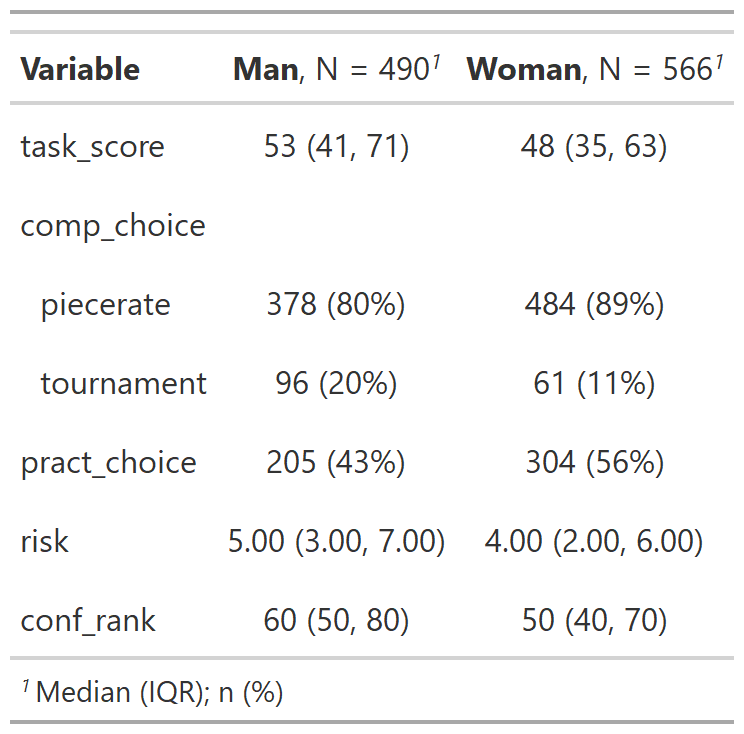
\includegraphics[width=0.5\linewidth]{C:/Users/keana/OneDrive - PennO365/Comp_transfer2018/Penn/practice_study/gender-practice/study1/figs/summary-table-gender-study1} \end{center}

\begin{table}[ht]
\centering
\begingroup\fontsize{0.1pt}{0.1pt}\selectfont
\begin{tabular}{r}
   \\ 
 \end{tabular}
\endgroup
\caption{Gender differences in the main variables of interest, including: task scores, choice to compete, choice to practice, confidence, and risk attitudes. Medians are reported for task score, risk attitudes, and confidence, with IQRs in parentheses. For choice to practice and choice to compete, we report the number and percentage of participants that fall into each category for each respective gender.} 
\label{tab:summary-table-gender-study1}
\end{table}

\newpage

\begin{center}
\includegraphics[width=1\linewidth]{C:/Users/keana/OneDrive - PennO365/Comp_transfer2018/Penn/practice_study/gender-practice/study1/figs/tab_task-scores-study1} \end{center}

\begin{table}[ht]
\centering
\begingroup\fontsize{0.1pt}{0.1pt}\selectfont
\begin{tabular}{r}
   \\ 
 \end{tabular}
\endgroup
\caption{All models are linear regressions with task score as the dependent variable, where man and piece-rate payment scheme are the reference categories for participant gender and competition choice, respectively. After controlling for risk attitudes, confidence, and competition choice, women still have lower scores on the multiplication task than men, p < .05 is considered significant and bolded.} 
\label{tab:tab-task-scores-study1}
\end{table}

\hypertarget{effects-of-knowledge-of-preparation-condition-on-gender-differences-in-choice-to-compete}{%
\subsubsection{Effects of knowledge of preparation condition on gender differences in choice to compete}\label{effects-of-knowledge-of-preparation-condition-on-gender-differences-in-choice-to-compete}}

Contrary to our predictions, we do not find evidence of a significant interaction between gender and condition on the decision to compete, \(b = 0.06\), 95\% CI \([-0.63\), \(0.76]\), \(z = 0.18\), \(p = .861\) (see Figure \ref{fig:s100}). When included as a sole predictor of the choice to compete in a logistic regression, we did not find evidence that assignment to the knowledge of preparation affected the choice to compete, \(b = 0.01\), 95\% CI \([-0.33\), \(0.35]\), \(z = 0.05\), \(p = .963\). Thus, the point estimate for the effect of the knowledge of preparation condition was positive and the 95\% CI did not include negative effects that were greater in magnitude than 0.33.

\begin{figure}

{\centering 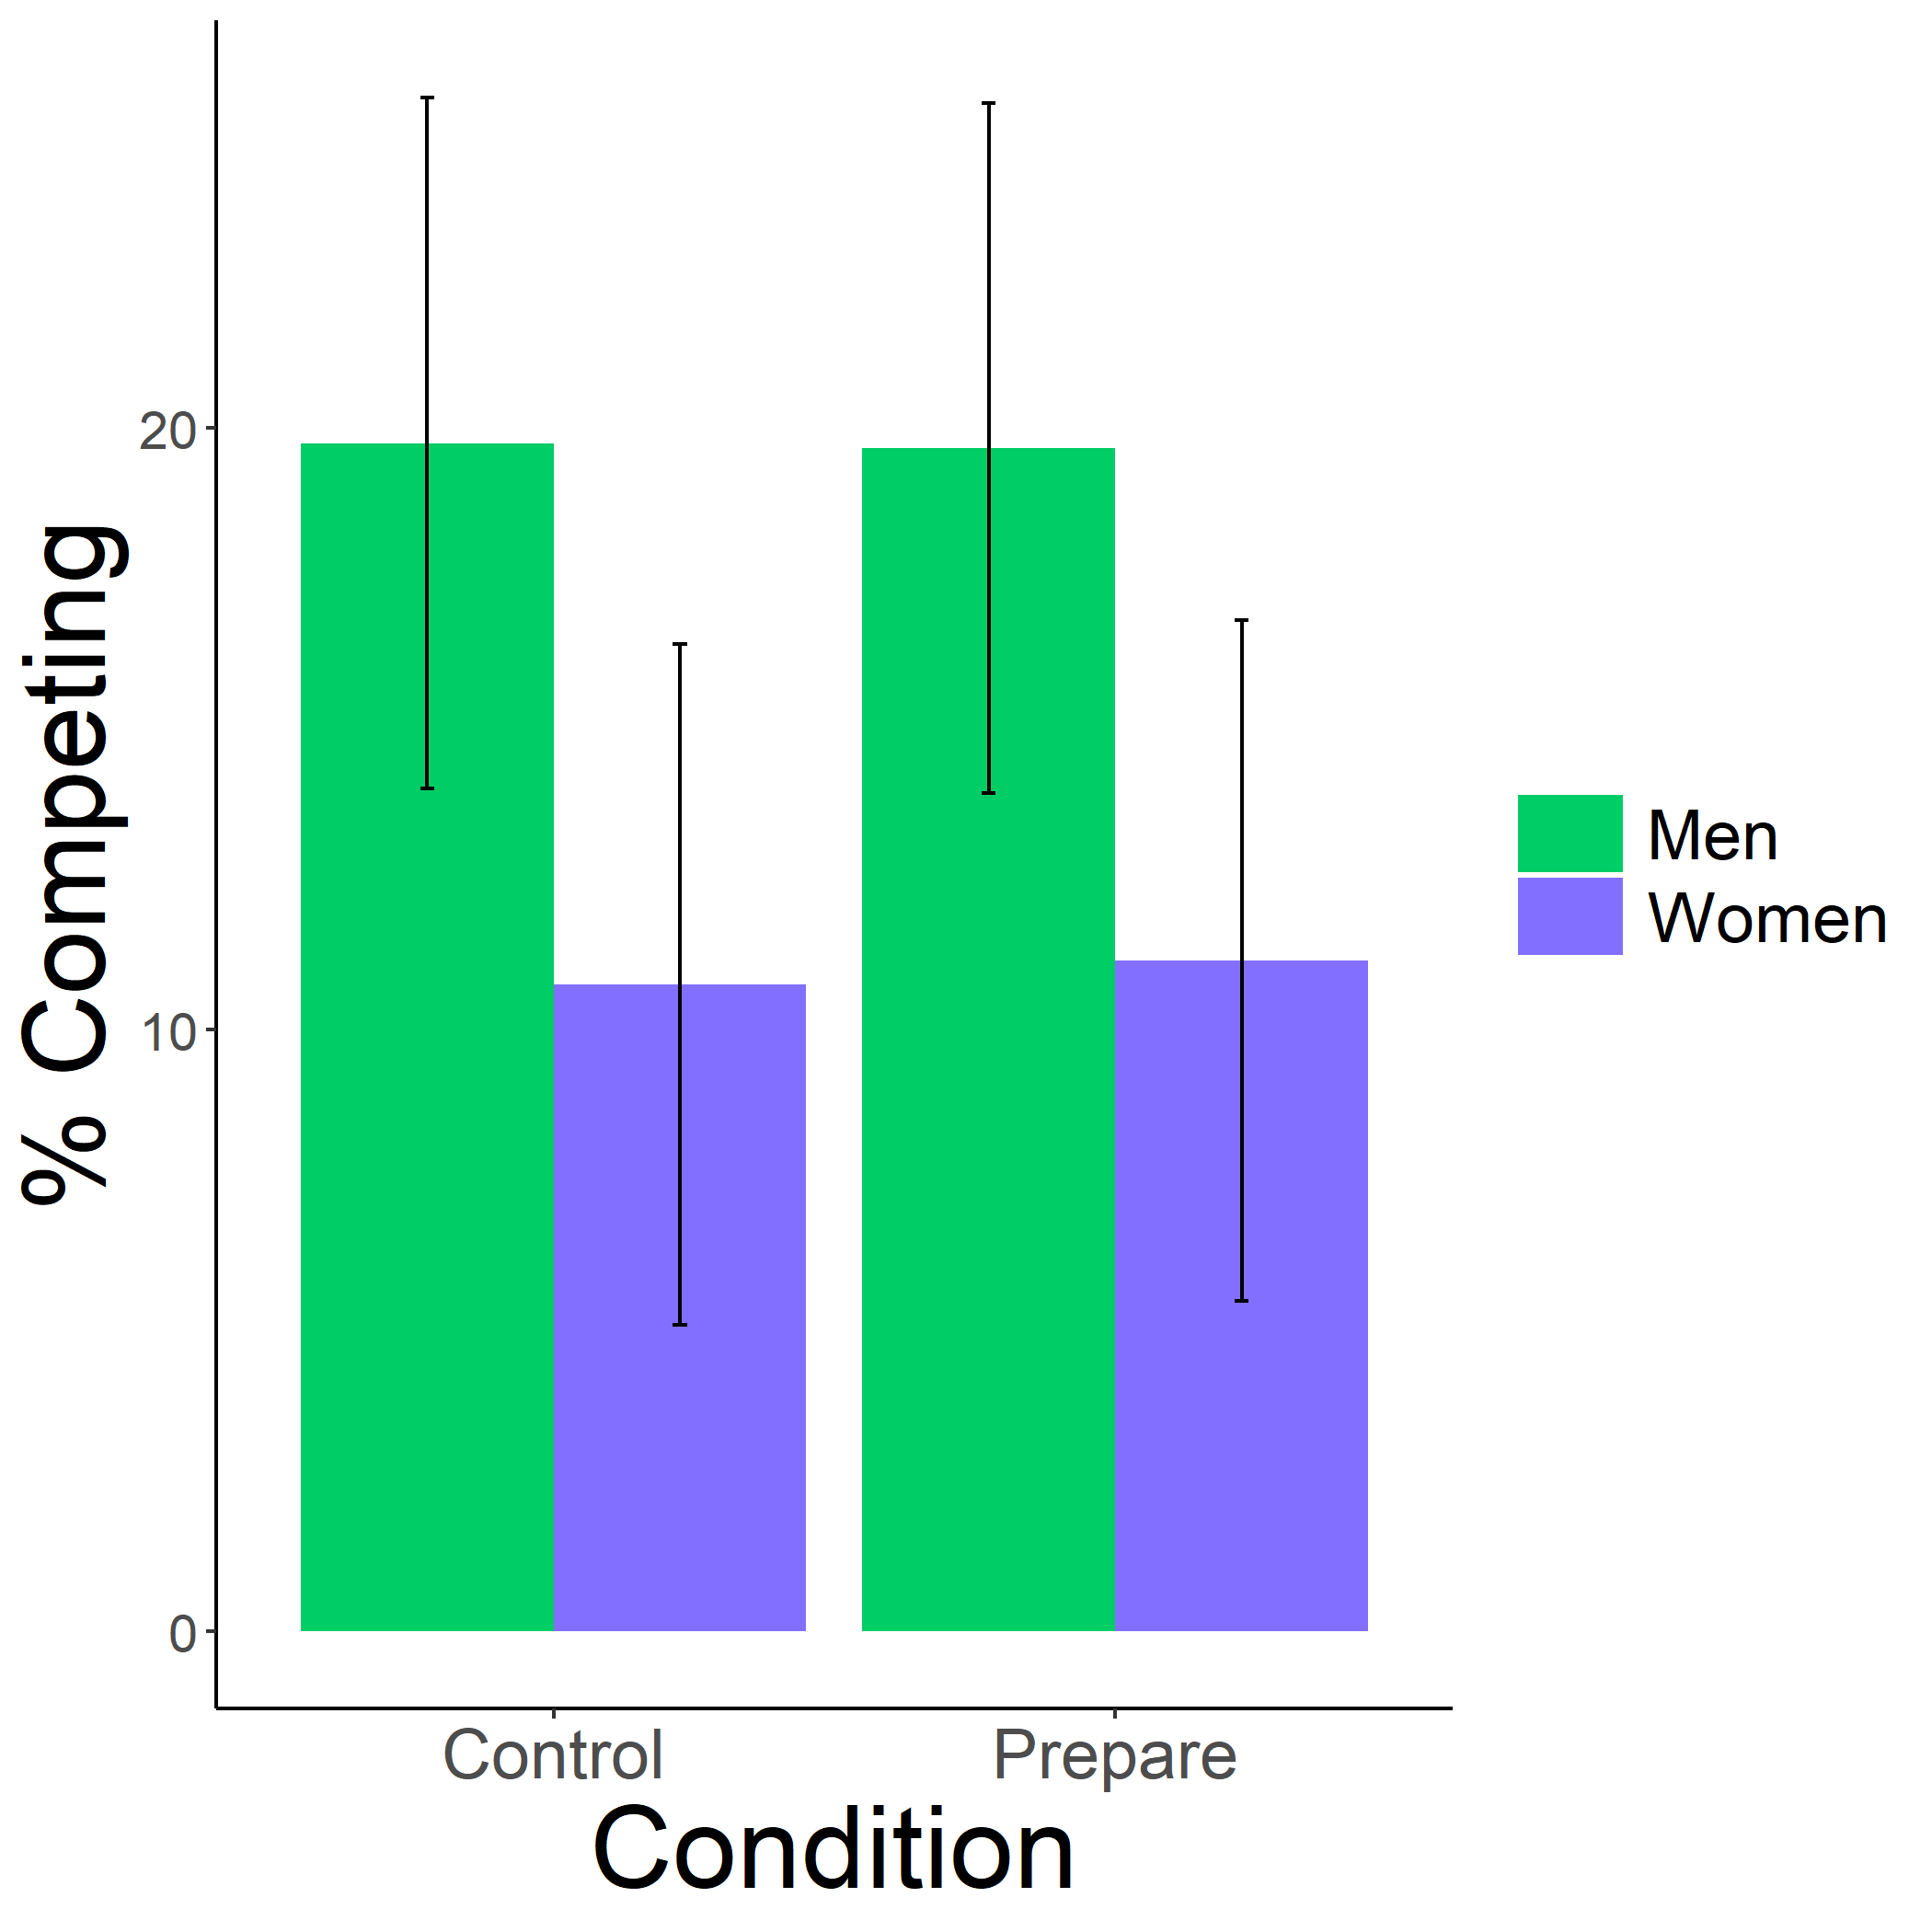
\includegraphics[width=300px]{C:/Users/keana/OneDrive - PennO365/Comp_transfer2018/Penn/practice_study/gender-practice/study1/figs/fig00_comp-choice-by-gender-and-cond-bar} 

}

\caption{Proportion of men and women in Study 1 who chose to compete based on preparation condition. Knowledge of preparation did not reduce the gender difference in competitiveness. Error bars represent standard errors.}\label{fig:s100}
\end{figure}

\hypertarget{gender-differences-in-preparation}{%
\subsubsection{Gender differences in preparation}\label{gender-differences-in-preparation}}

As hypothesized, a logistic regression with gender predicting the choice to practice shows that a greater proportion of women (55.88\%) took advantage of the opportunity to practice relative to men (43.25\%), \(b = 0.51\), 95\% CI \([0.26\), \(0.76]\), \(z = 4.01\), \(p < .001\) (see right panel of Figure \ref{fig:panel-study1}). Gender remains a significant predictor of the binary choice to prepare after adding participants' choice to compete and the interaction between gender and the choice to compete in the model, \(b = 0.54\), 95\% CI \([0.27\), \(0.82]\), \(z = 3.92\), \(p < .001\), but we do not find an interaction between gender and the choice to compete, (see left panel of Figure \ref{fig:panel-study1}). We also find that the choice to compete positively predicts a participants' likelihood of choosing to practice, \(b = 0.50\), 95\% CI \([0.05\), \(0.95]\), \(z = 2.18\), \(p = .030\). In a subsequent logistic regression with additional possible predictors of the decision to practice, we find that the gender effect holds, \(b = 0.55\), 95\% CI \([0.27\), \(0.84]\), \(z = 3.79\), \(p < .001\), suggesting that it is not explained by the observed gender differences in risk attitudes, confidence, nor task scores (see Table \ref{tab:tab-pract-choice-study1}). We also ran a two-part hurdle model with gender, competition choice, and the interaction between those variables predicting the number of practice rounds variable with the assumption that there may be different decision-making processes underlying the choice to prepare when first offered the opportunity versus the choice to continue preparing thereafter. However, we do not find evidence of gender differences in the choice to continue preparing after the initial decision to prepare - that is, the gender predictor in the count part of the model did not show a significant effect on the dependent variable, \emph{b} = 0.11, 95\% CI {[}-0.12, 0.34{]}, \emph{z} = 0.96, \emph{p} = 0.34.

\begin{figure}

{\centering 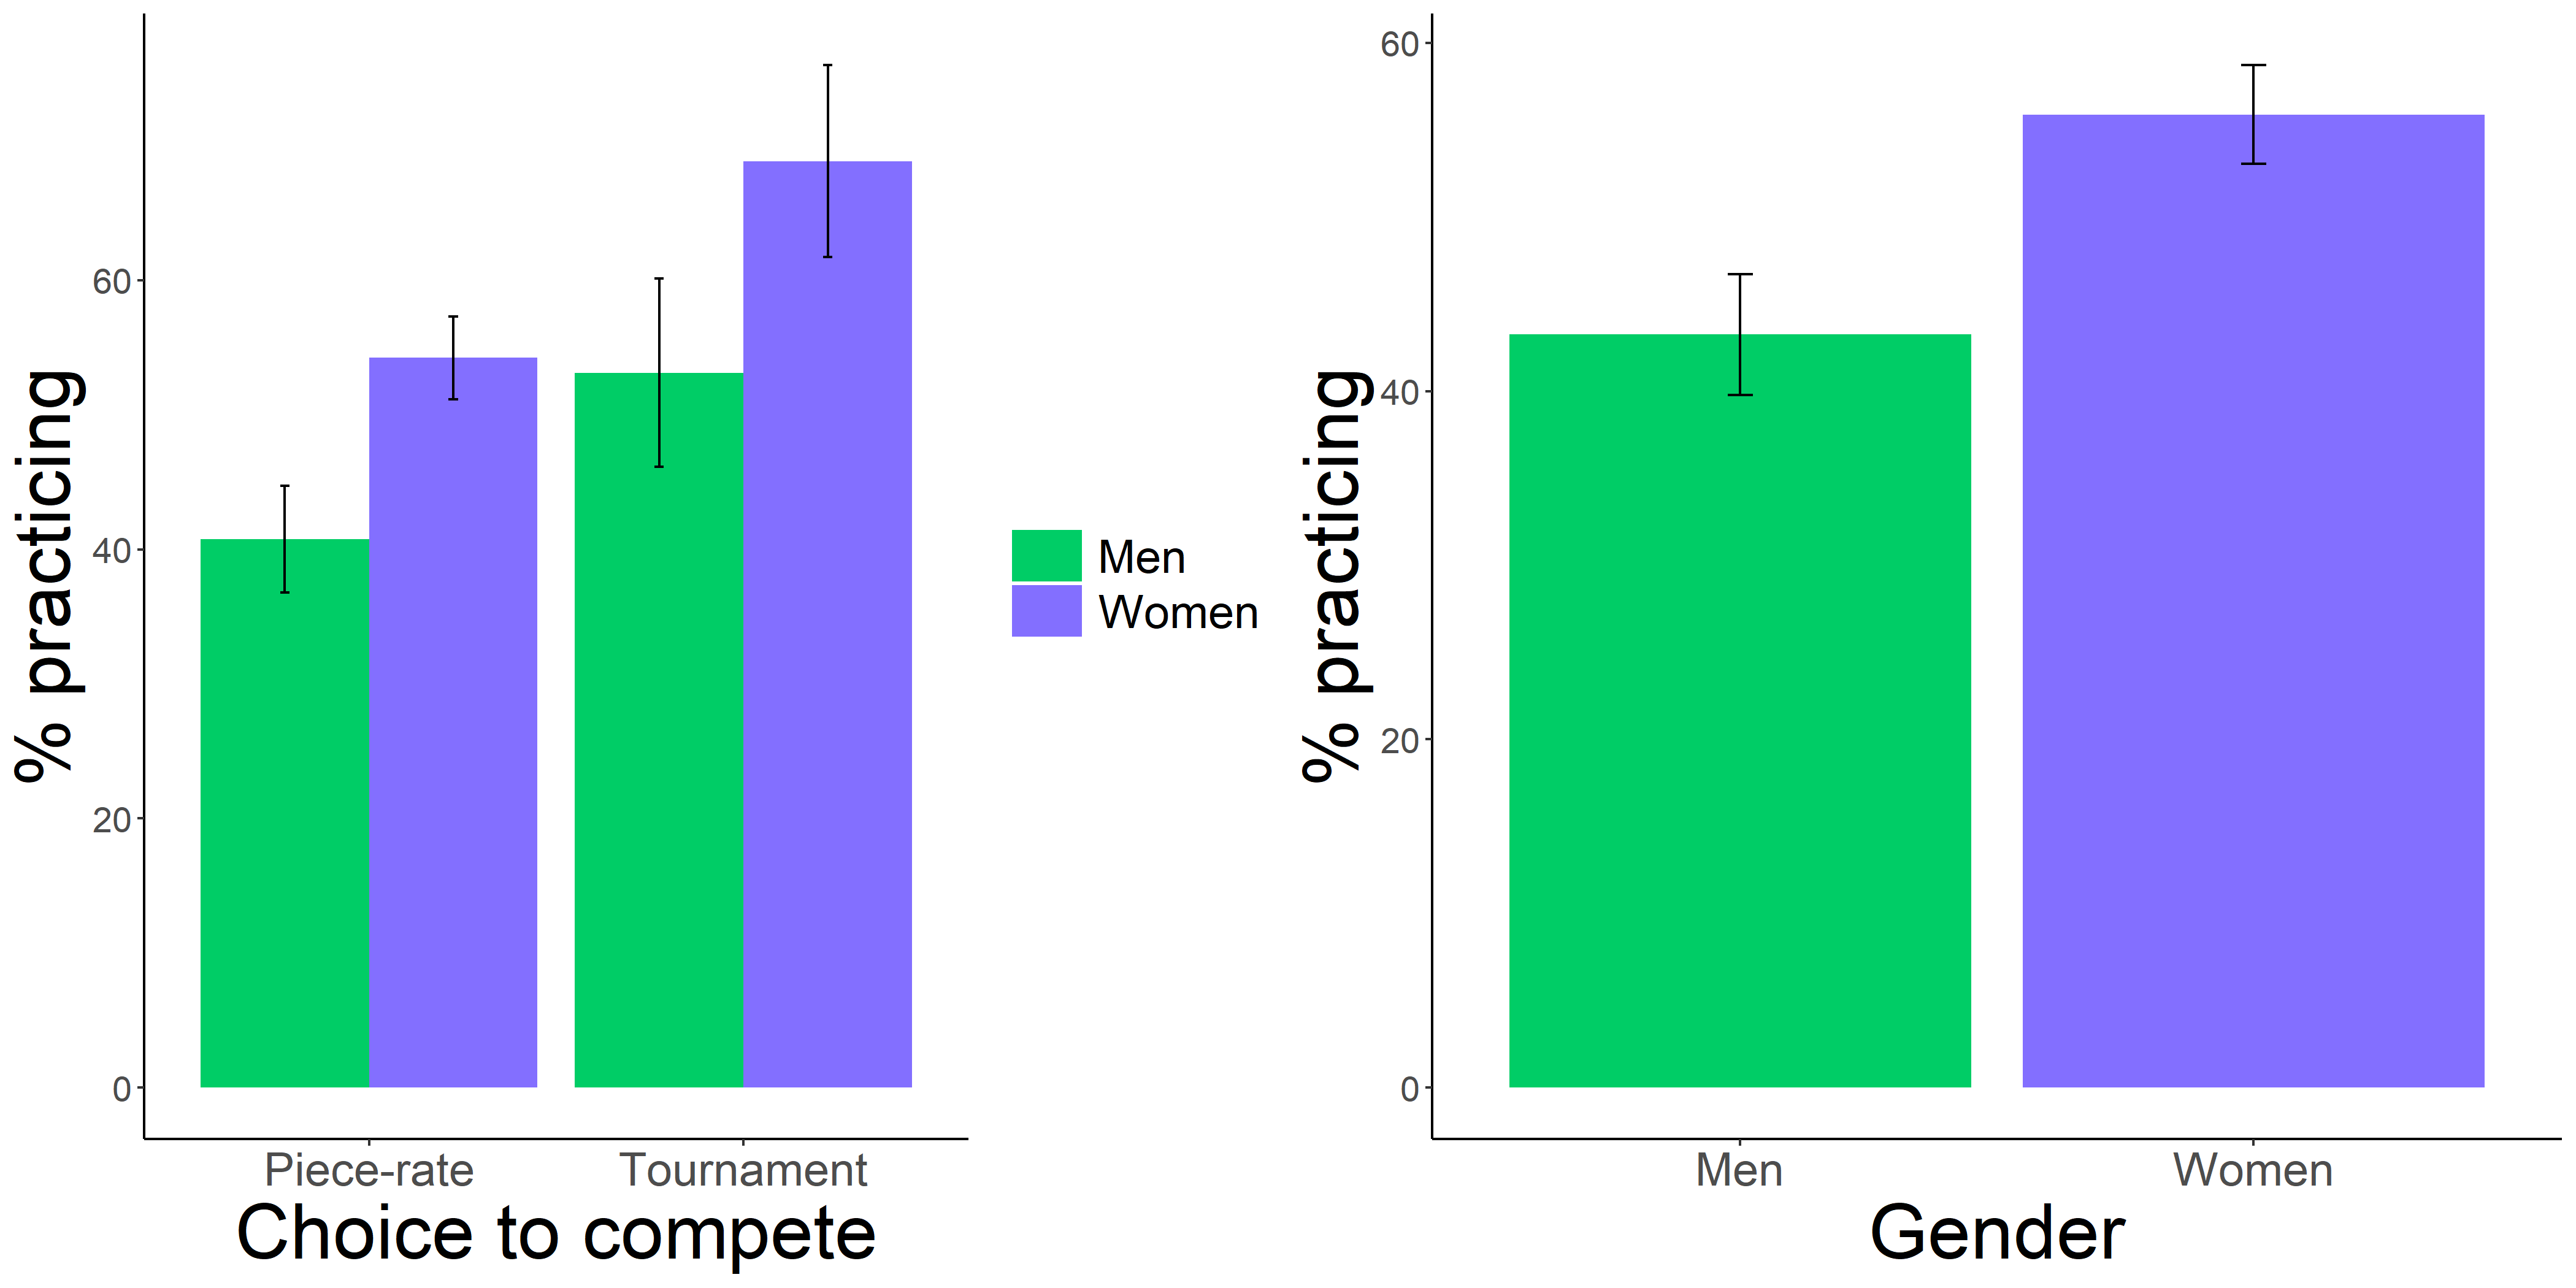
\includegraphics[width=1\linewidth]{C:/Users/keana/OneDrive - PennO365/Comp_transfer2018/Penn/practice_study/gender-practice/study1/figs/panel_study1} 

}

\caption{Right panel shows the proportion of men and women in Study 1 who chose to prepare. Left panel shows the proportion of men and women in Study 1 who chose to prepare based on choice to compete. Women choose to prepare more than men, regardless of their decision to compete. Error bars represent standard errors.}\label{fig:panel-study1}
\end{figure}

\newpage

\begin{center}
\includegraphics[width=1\linewidth]{C:/Users/keana/OneDrive - PennO365/Comp_transfer2018/Penn/practice_study/gender-practice/study1/figs/tab_pract-choice-study1} \end{center}

\begin{table}[ht]
\centering
\begingroup\fontsize{0.1pt}{0.1pt}\selectfont
\begin{tabular}{r}
   \\ 
 \end{tabular}
\endgroup
\caption{All models are logistic regressions with choice to prepare as the dependent variable, where man and piece-rate payment scheme are the reference categories for participant gender and competition choice, respectively. Women prepare more than men regardless of competition choice, task score, risk attitudes, or confidence. p < .05 is considered significant and bolded.} 
\label{tab:tab-pract-choice-study1}
\end{table}

\hypertarget{perceptions-of-gender-differences-in-preparation-performance-and-competitiveness}{%
\subsubsection{Perceptions of gender differences in preparation, performance, and competitiveness}\label{perceptions-of-gender-differences-in-preparation-performance-and-competitiveness}}

This gender difference in preparation aligned with participants' incentivized predictions about gender differences in preparation, where a greater proportion of participants (83.37\%) expected women to spend more time preparing for the multiplication task, \(\chi^2(1, n = 1056) = 447.11\), \(p < .001\) (see Figure \ref{fig:s103}). They also expected women to prepare more in general, \(\chi^2(1, n = 1056) = 625.06\), \(p < .001\), with 89.51\% indicating women prepare more in general versus 10.49\% indicating that men prepare more in general (see Figure \ref{fig:s106}). However, participants did not expect any gender differences in performance on the task, \(\chi^2(1, n = 1056) = 1.02\), \(p = .313\) (see Figure \ref{fig:s104}). Additionally, participants accurately predicted that women were less likely to choose to compete, \(\chi^2(1, n = 1056) = 716.24\), \(p < .001\) (see Figure \ref{fig:s105}). See Table \ref{tab:summary-table-beliefs-study1}) for a summary of participants' responses to the questions about gender differences in preparation, performance, and competitiveness.

\begin{center}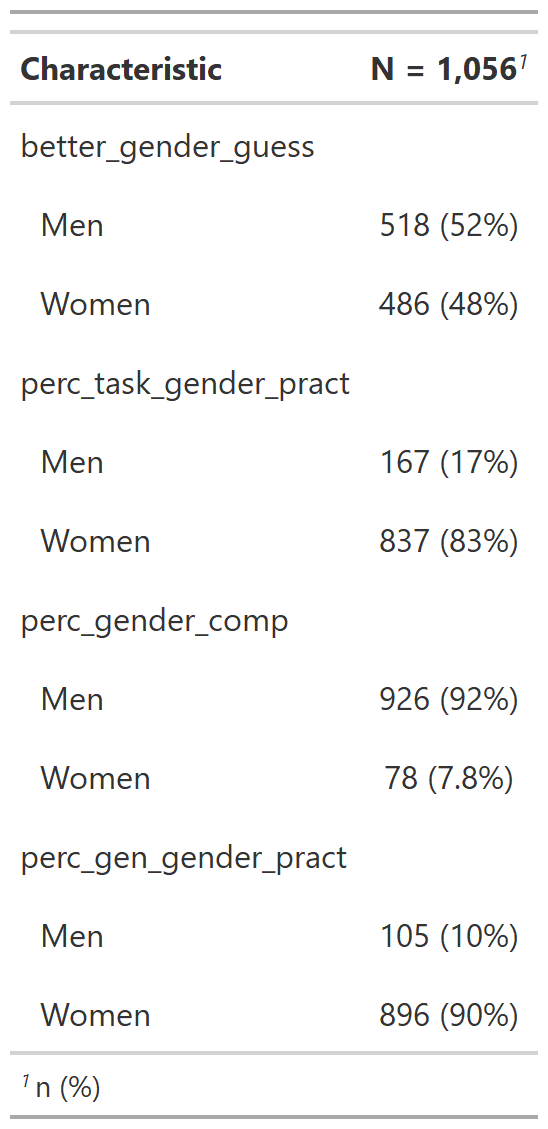
\includegraphics[width=0.35\linewidth]{C:/Users/keana/OneDrive - PennO365/Comp_transfer2018/Penn/practice_study/gender-practice/study1/figs/summary-table-beliefs-study1} \end{center}

\begin{table}[ht]
\centering
\begingroup\fontsize{0.1pt}{0.1pt}\selectfont
\begin{tabular}{r}
   \\ 
 \end{tabular}
\endgroup
\caption{Number and percentage of participants that selected each respective option when asked which gender would correctly solve more problems on the multiplication task, spend more time preparing for the multiplication task, choose the tournament payment scheme more often, and spend more time preparing on most tasks.} 
\label{tab:summary-table-beliefs-study1}
\end{table}

\begin{figure}

{\centering 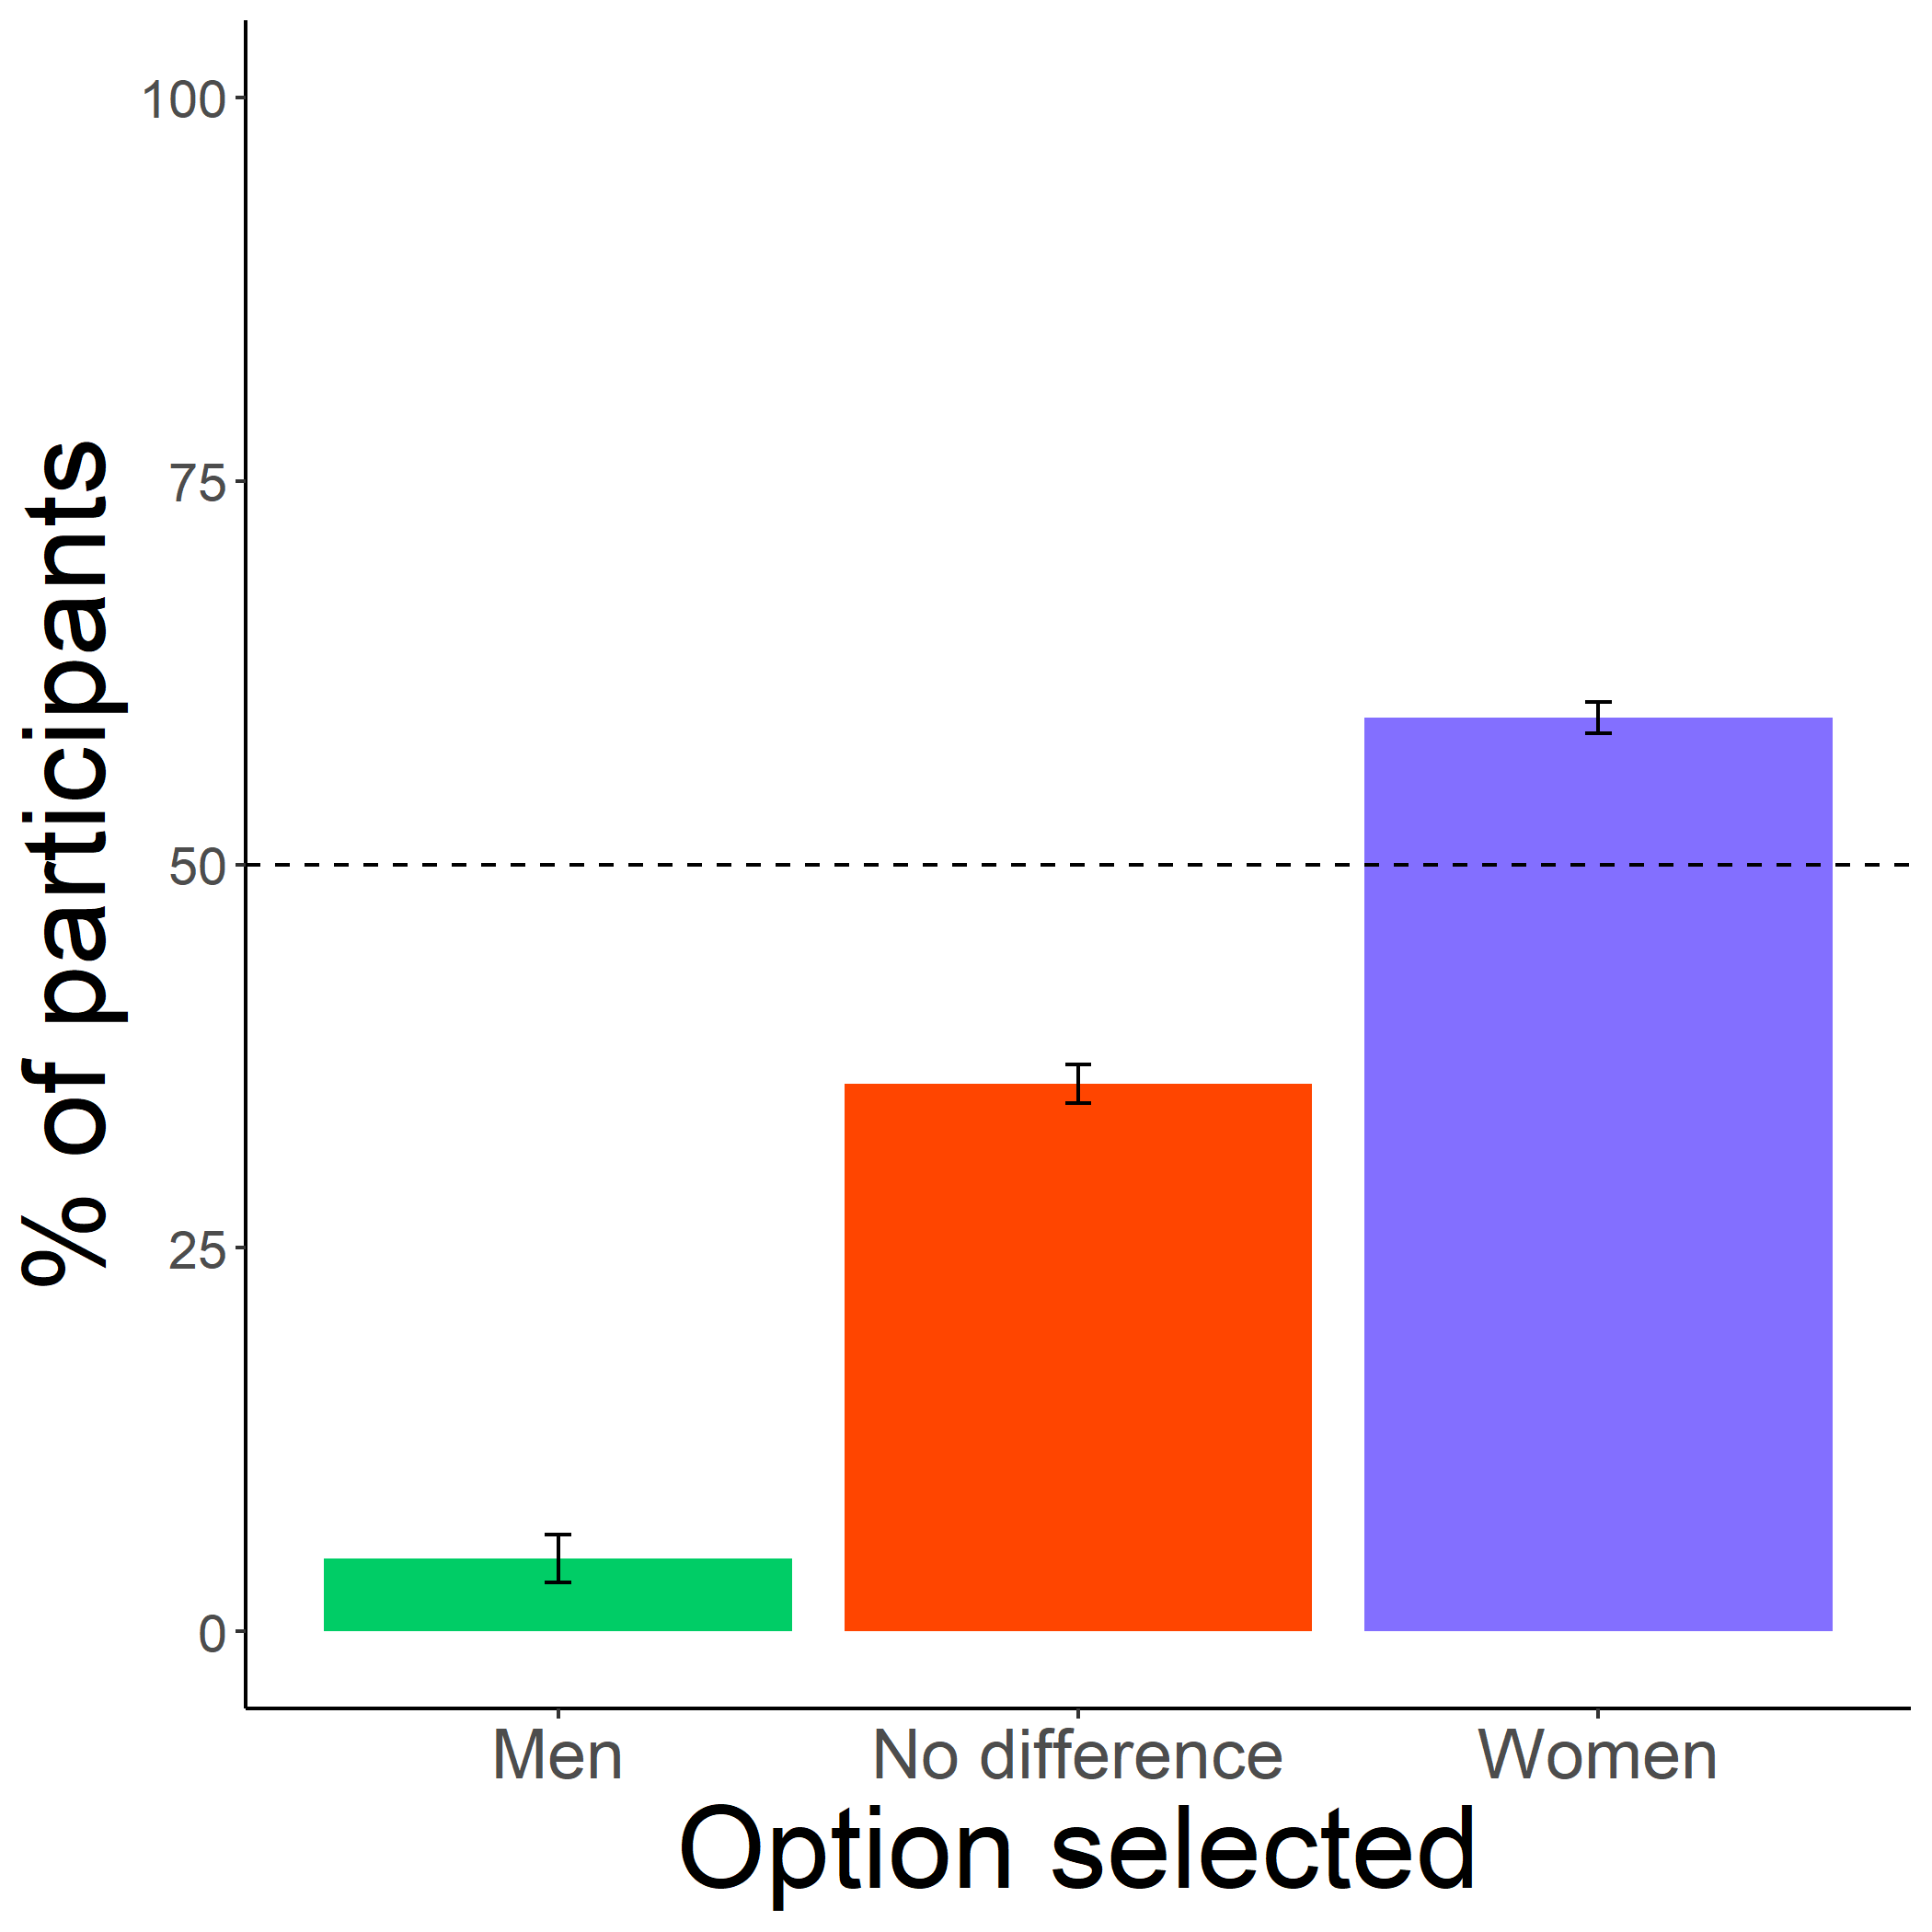
\includegraphics[width=300px]{C:/Users/keana/OneDrive - PennO365/Comp_transfer2018/Penn/practice_study/gender-practice/study1/figs/fig03_perc-task-gender-pract} 

}

\caption{Proportion of participants that predicted women or men would spend more time preparing for the multiplication task. A significantly larger proportion of participants expected women to spend more time preparing for the multiplication task. Error bars represent standard errors.}\label{fig:s103}
\end{figure}

\begin{figure}

{\centering 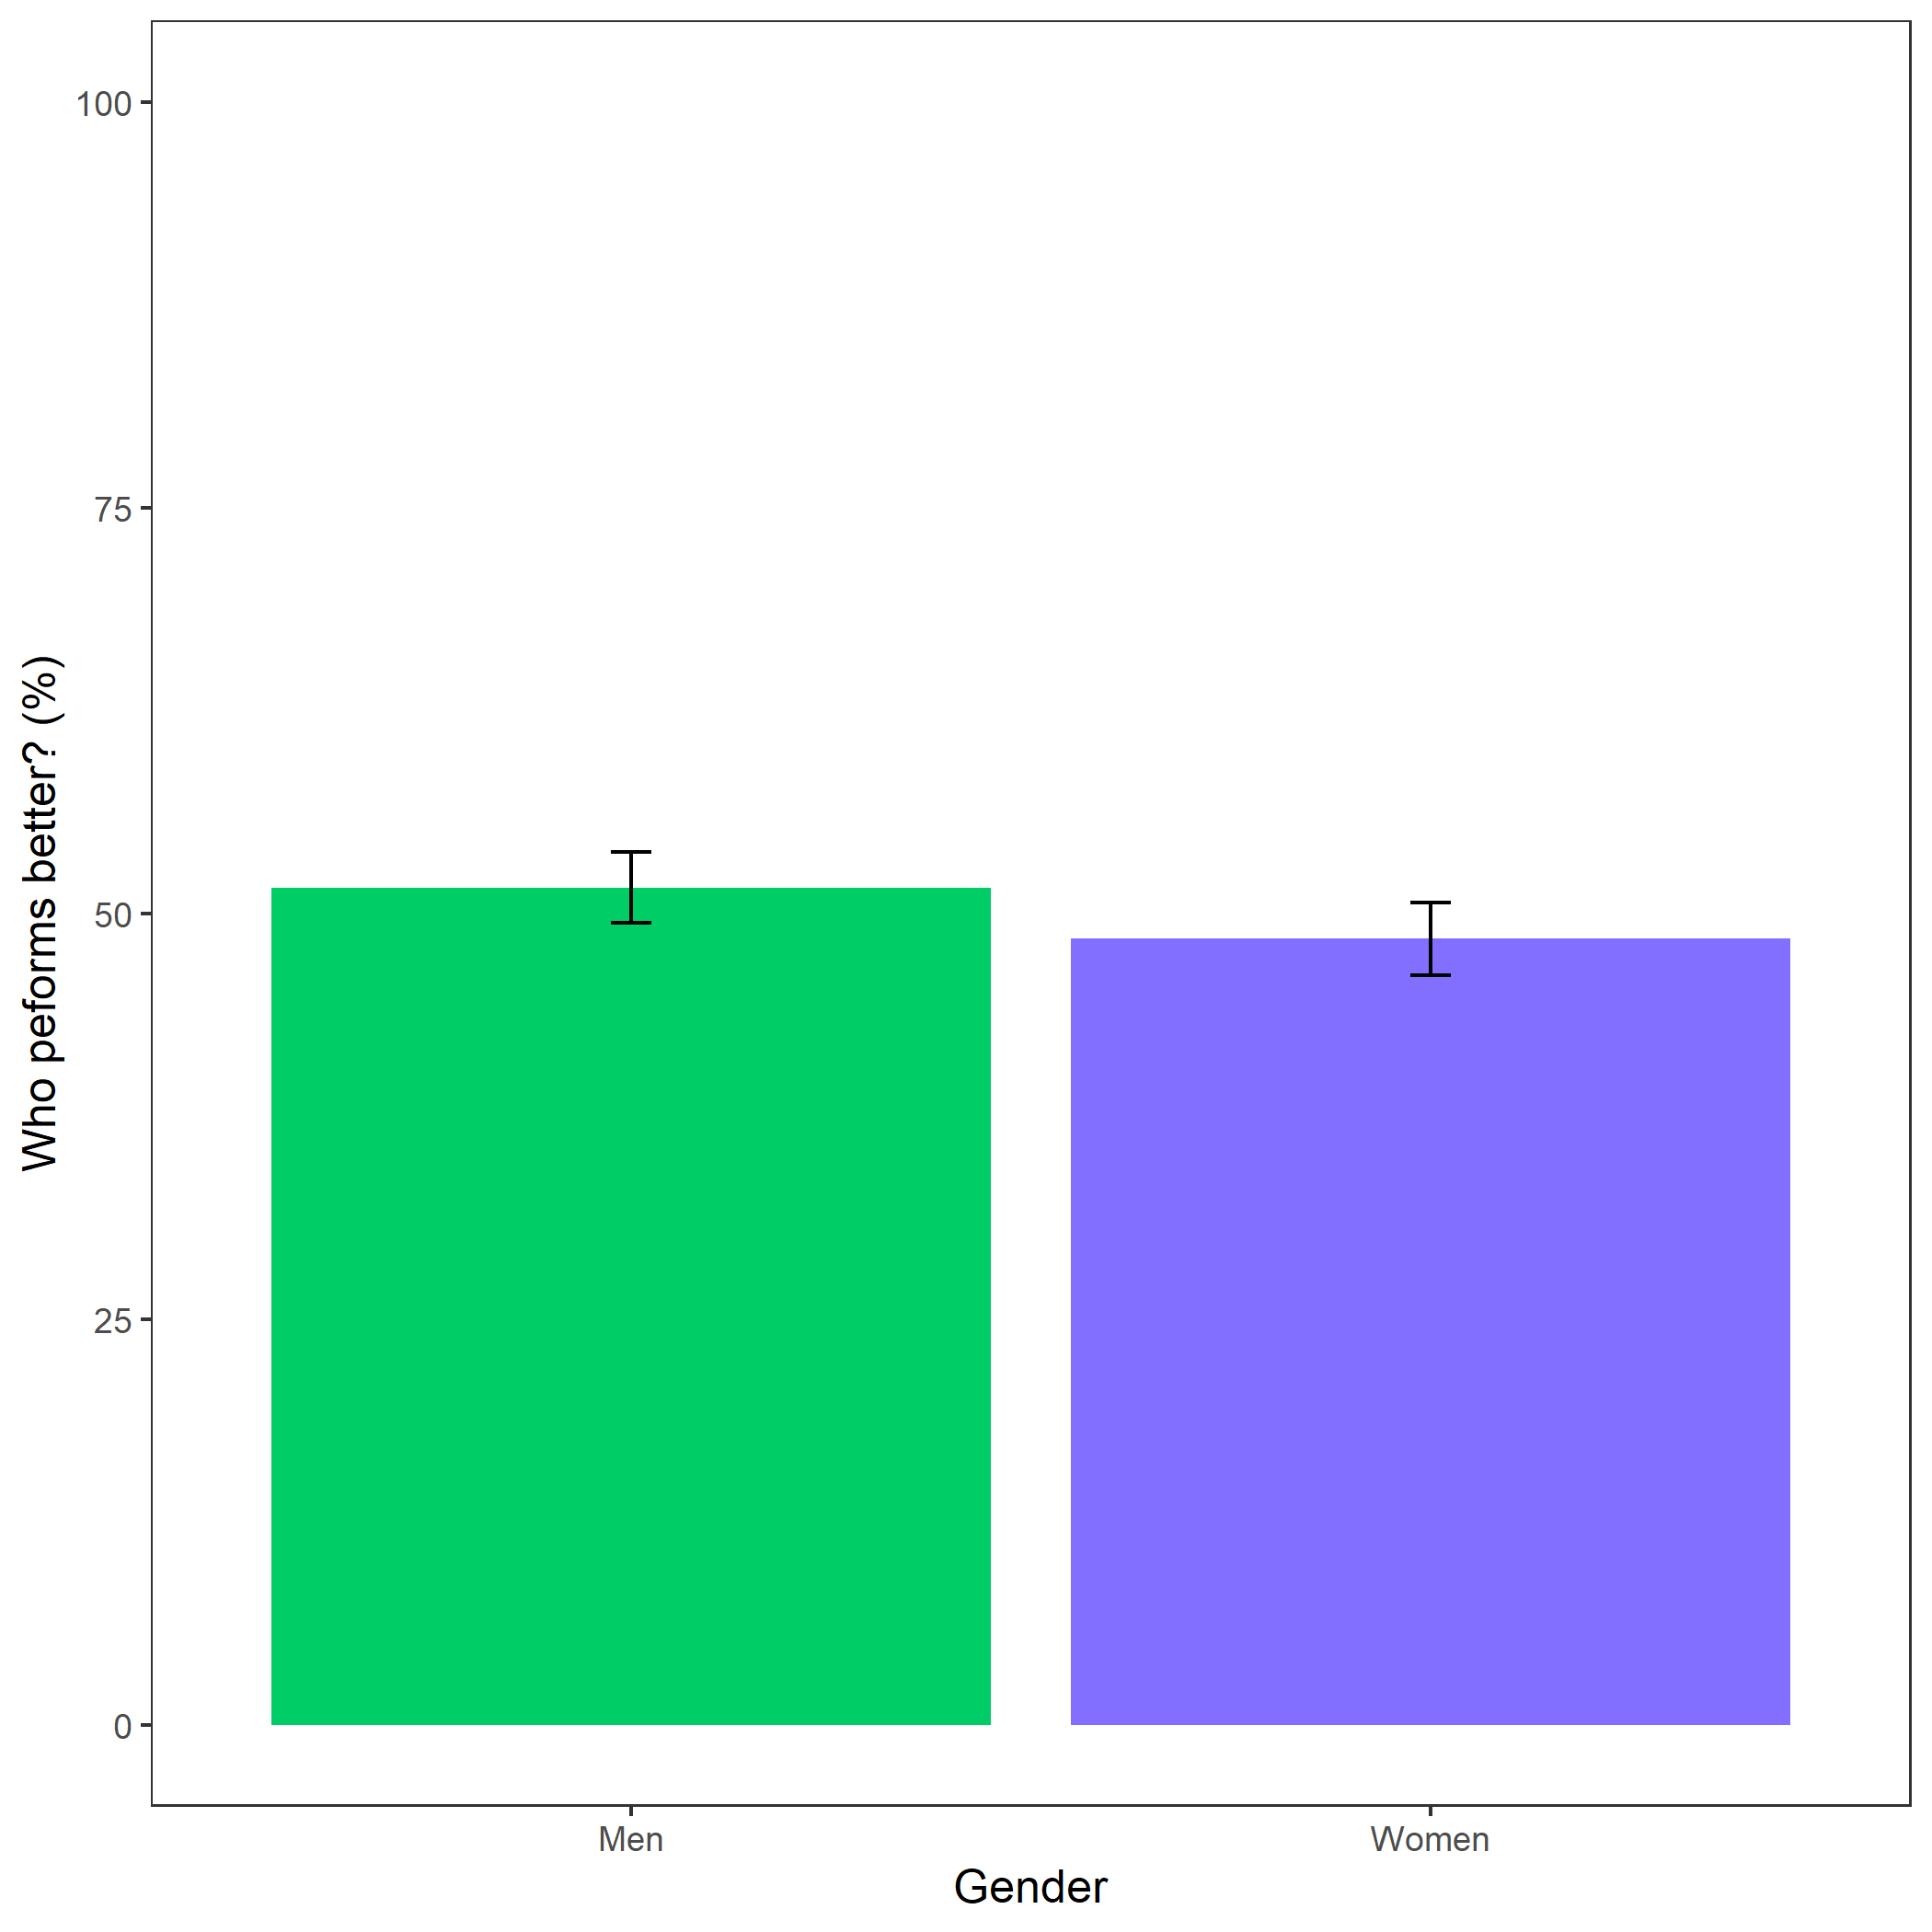
\includegraphics[width=300px]{C:/Users/keana/OneDrive - PennO365/Comp_transfer2018/Penn/practice_study/gender-practice/study1/figs/fig04_better-gender-guess} 

}

\caption{Proportion of participants that predicted women or men would correctly solve more problems on the multiplication task. There was no significant difference in the proportion of participants that expected women or men to perform better on the multiplication task. Error bars represent standard errors.}\label{fig:s104}
\end{figure}

\begin{figure}

{\centering 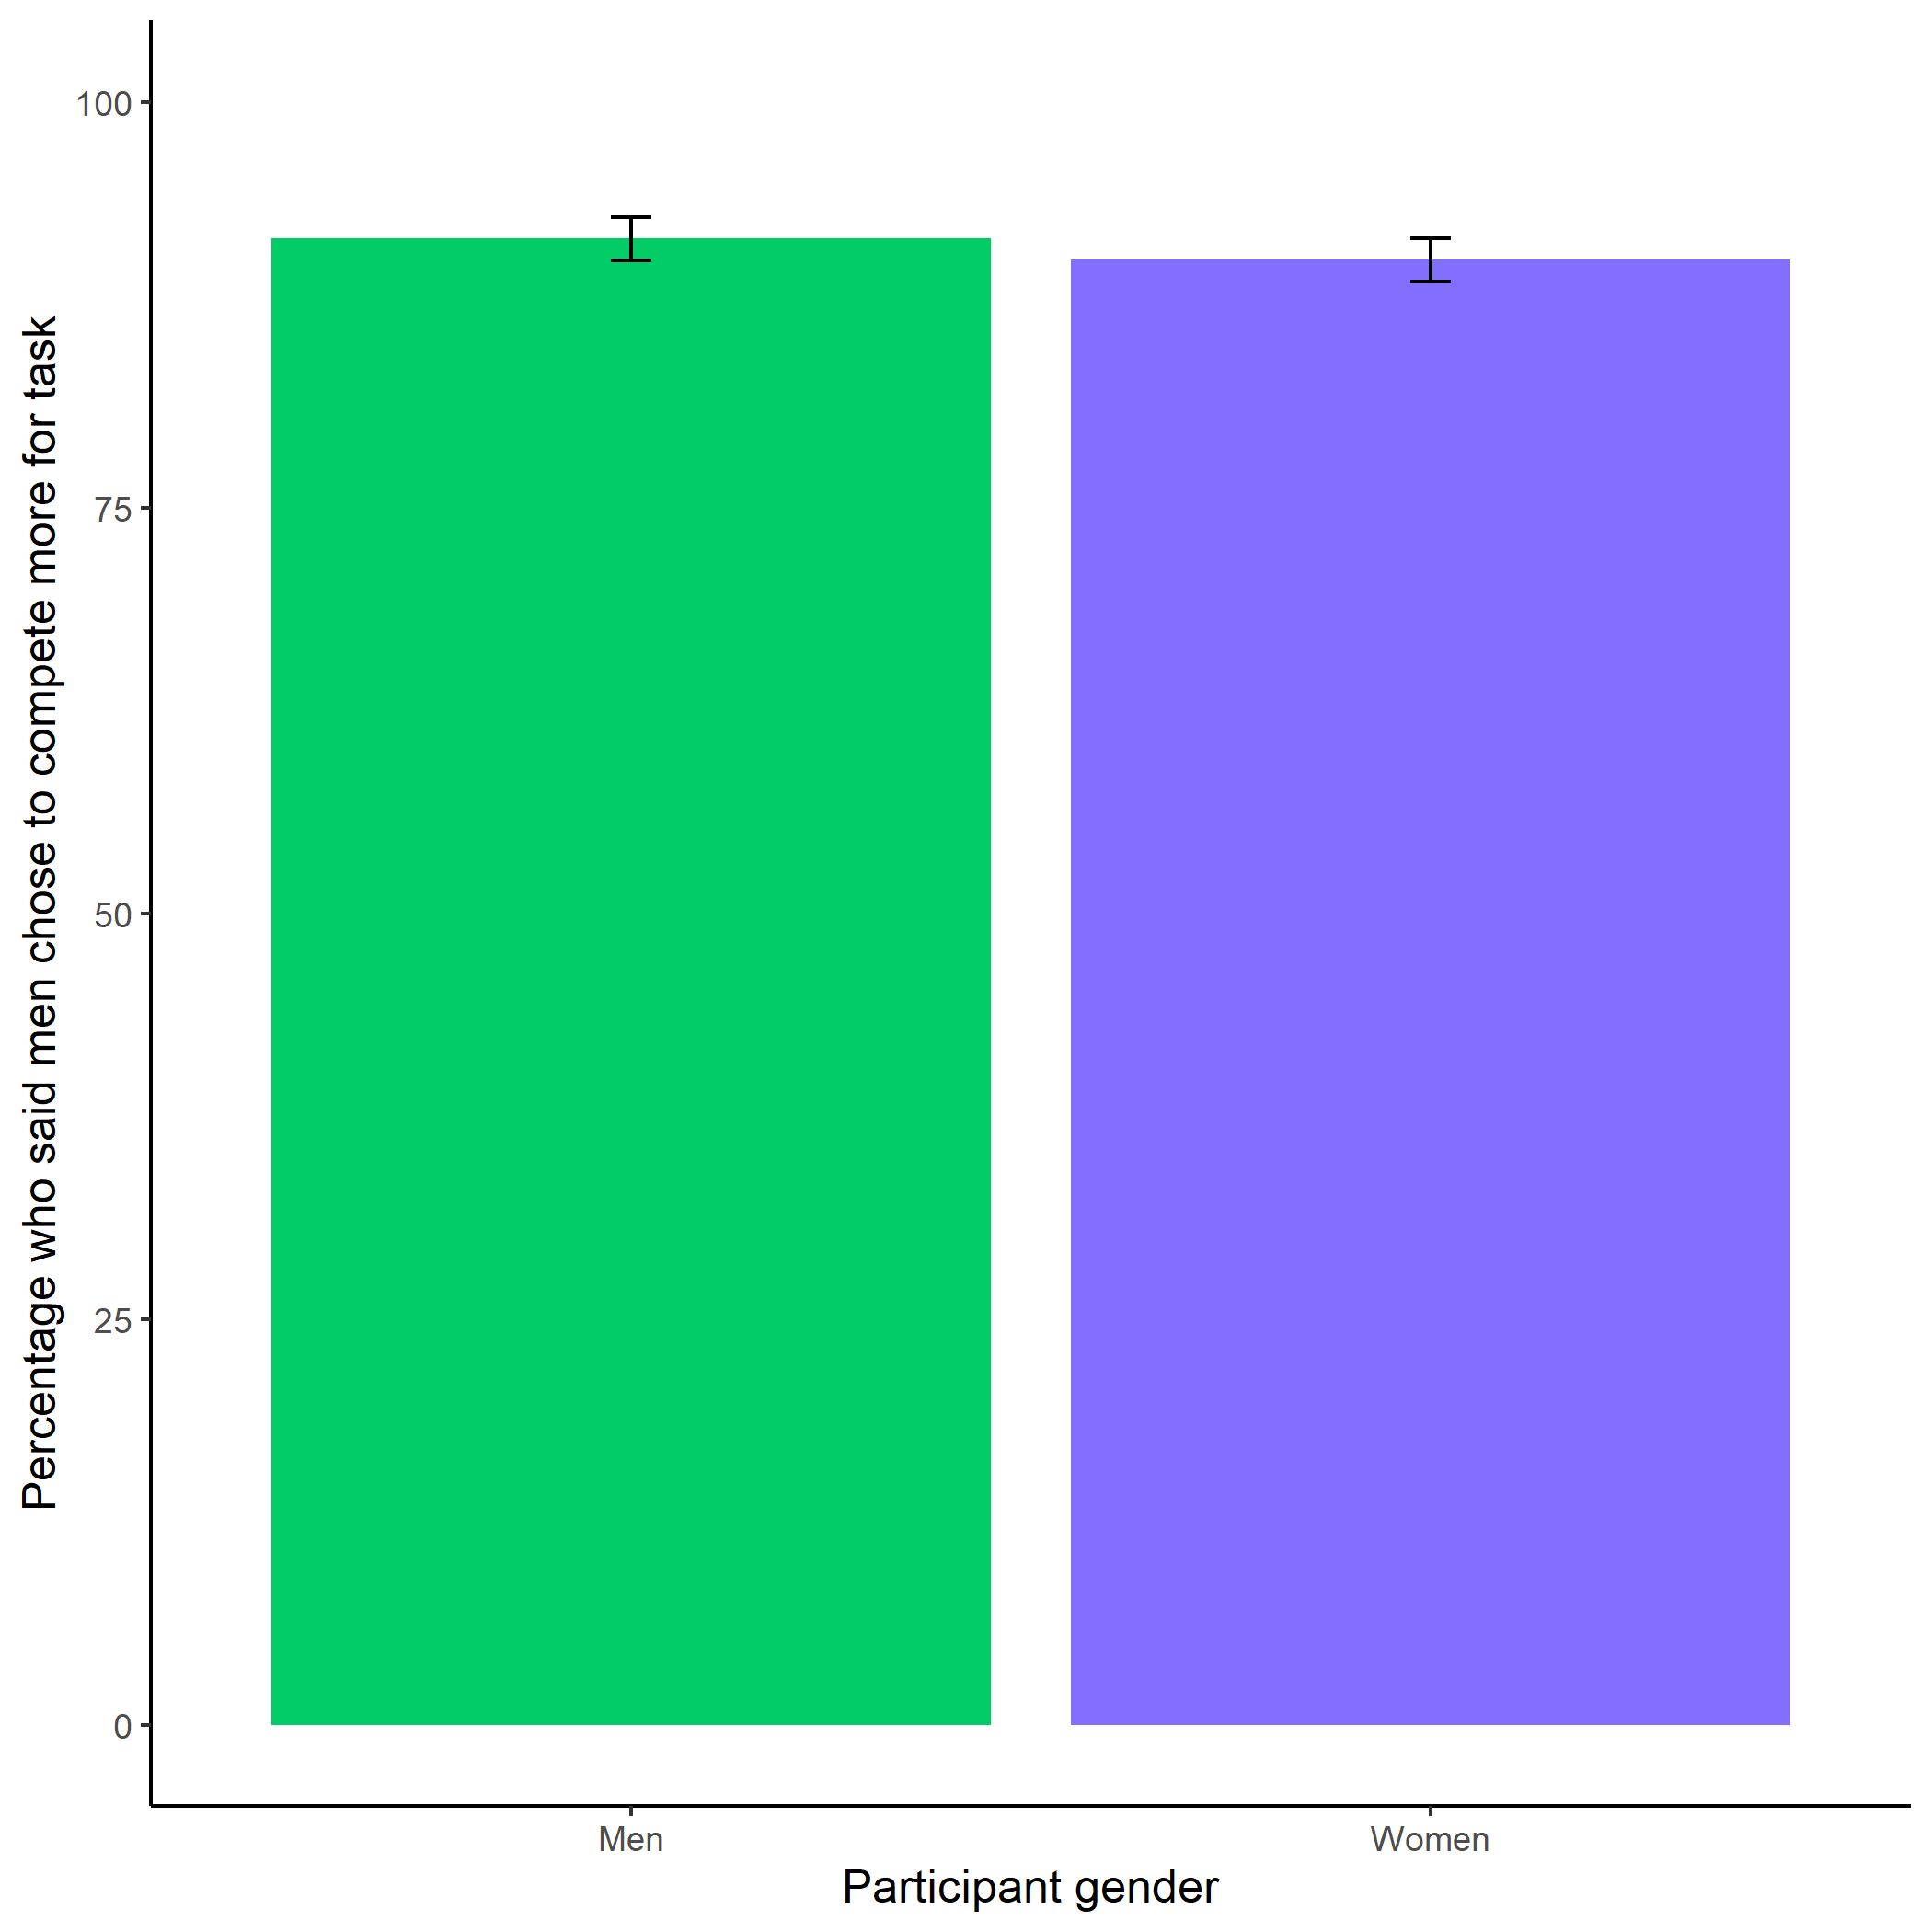
\includegraphics[width=300px]{C:/Users/keana/OneDrive - PennO365/Comp_transfer2018/Penn/practice_study/gender-practice/study1/figs/fig05_perc-gender-comp} 

}

\caption{Proportion of participants that predicted women or men would choose the tournament payment scheme more often. A significantly larger proportion of participants expected men to be more likely to choose to compete. Error bars represent standard errors.}\label{fig:s105}
\end{figure}

\begin{figure}

{\centering 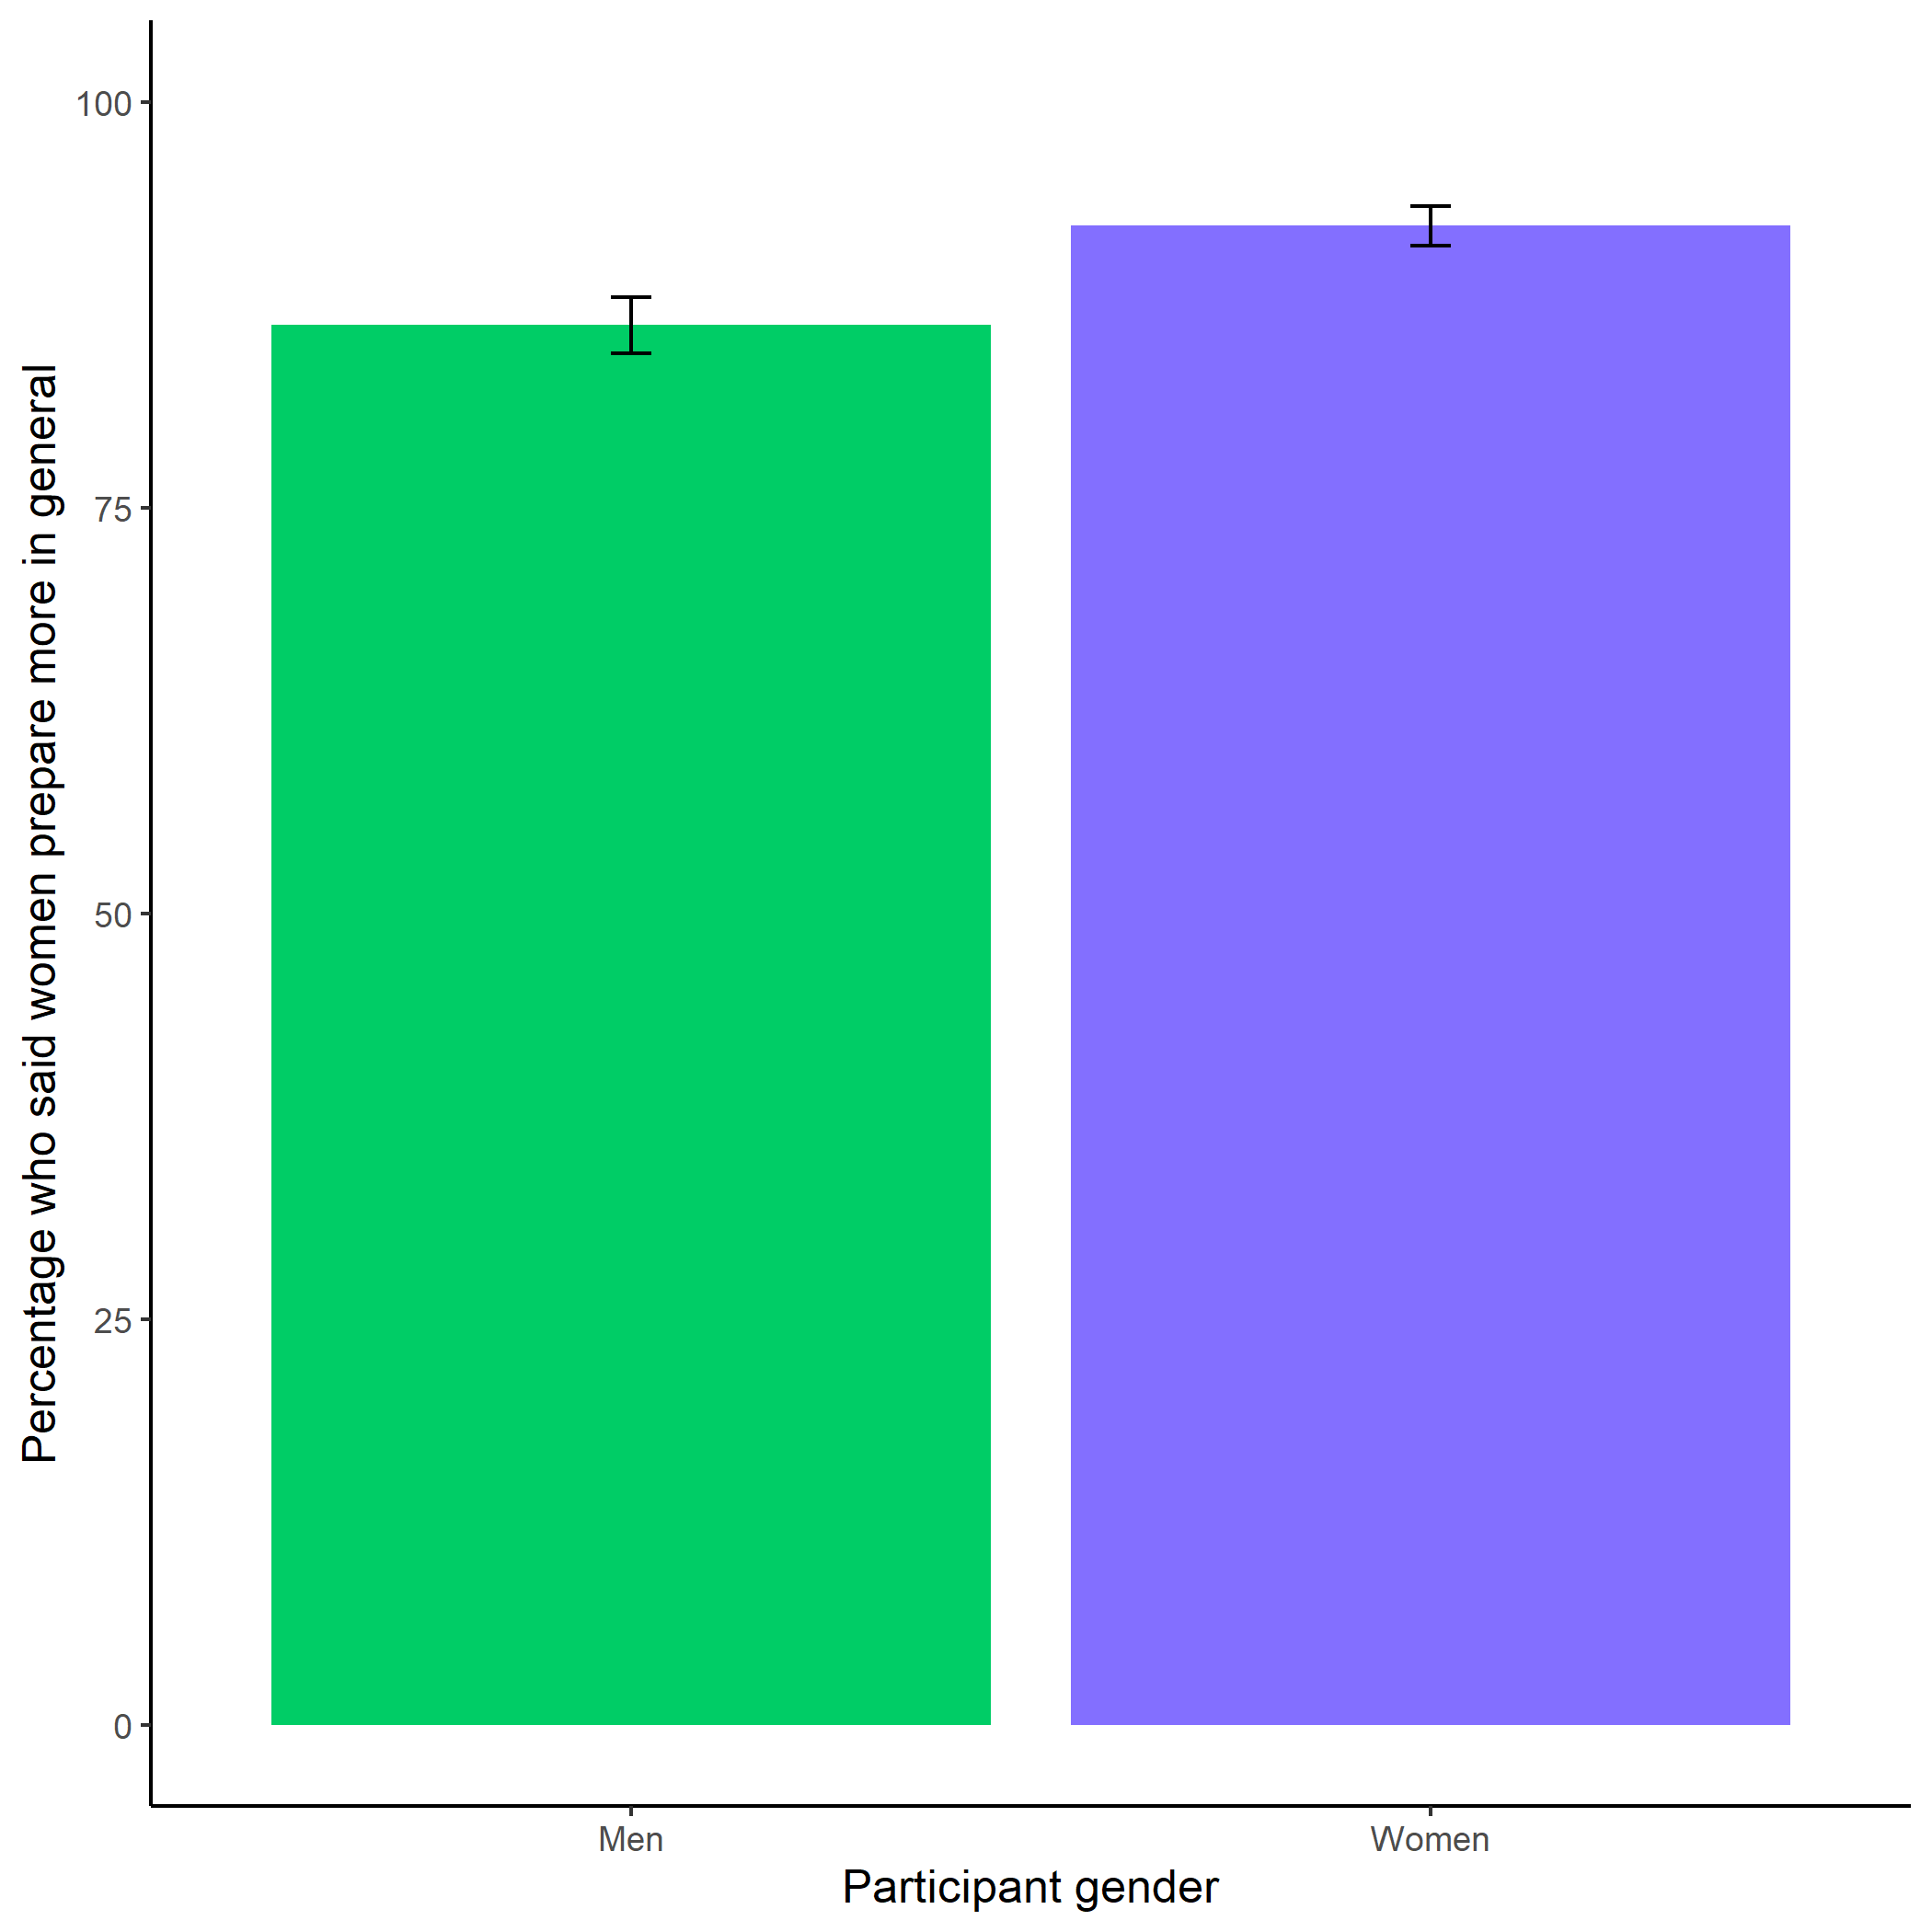
\includegraphics[width=300px]{C:/Users/keana/OneDrive - PennO365/Comp_transfer2018/Penn/practice_study/gender-practice/study1/figs/fig06_perc-gen-gender-pract} 

}

\caption{Proportion of participants that predicted women or men would spend more time preparing on most tasks. A significantly larger proportion of participants expected women to spend more time preparing on most tasks. Error bars represent standard errors.}\label{fig:s106}
\end{figure}

\hypertarget{effects-of-gender-and-perceptions-on-practicing}{%
\subsubsection{Effects of gender and perceptions on practicing}\label{effects-of-gender-and-perceptions-on-practicing}}

Given our evidence that women choose to prepare more and that participants believe women choose to prepare more, we explored whether women who believed other women prepare more were especially likely to prepare. To that end, we ran a logistic regression with the choice to practice as the dependent variable and gender, beliefs about gender differences in preparation on most tasks, and the interaction between those two variables as the predictors. We find that women who said women generally prepare more on most tasks were especially likely to prepare, \(b = 1.00\), 95\% CI \([0.16\), \(1.85]\), \(z = 2.33\), \(p = .020\) (see Figure \ref{fig:pract-choice-by-gender-and-perc-gen-prep-bar-study1}). We ran a nearly identical analysis with participants' beliefs about gender differences in preparation for the multiplication task, gender, and the interaction between the two as predictors instead, and replicate the interaction effect, \(b = 0.77\), 95\% CI \([0.08\), \(1.46]\), \(z = 2.19\), \(p = .029\), such that women who said women spent more time preparing for the multiplication task were especially likely to prepare (see Figure \ref{fig:pract-choice-by-gender-and-perc-task-prep-bar-study1}).

\begin{figure}

{\centering 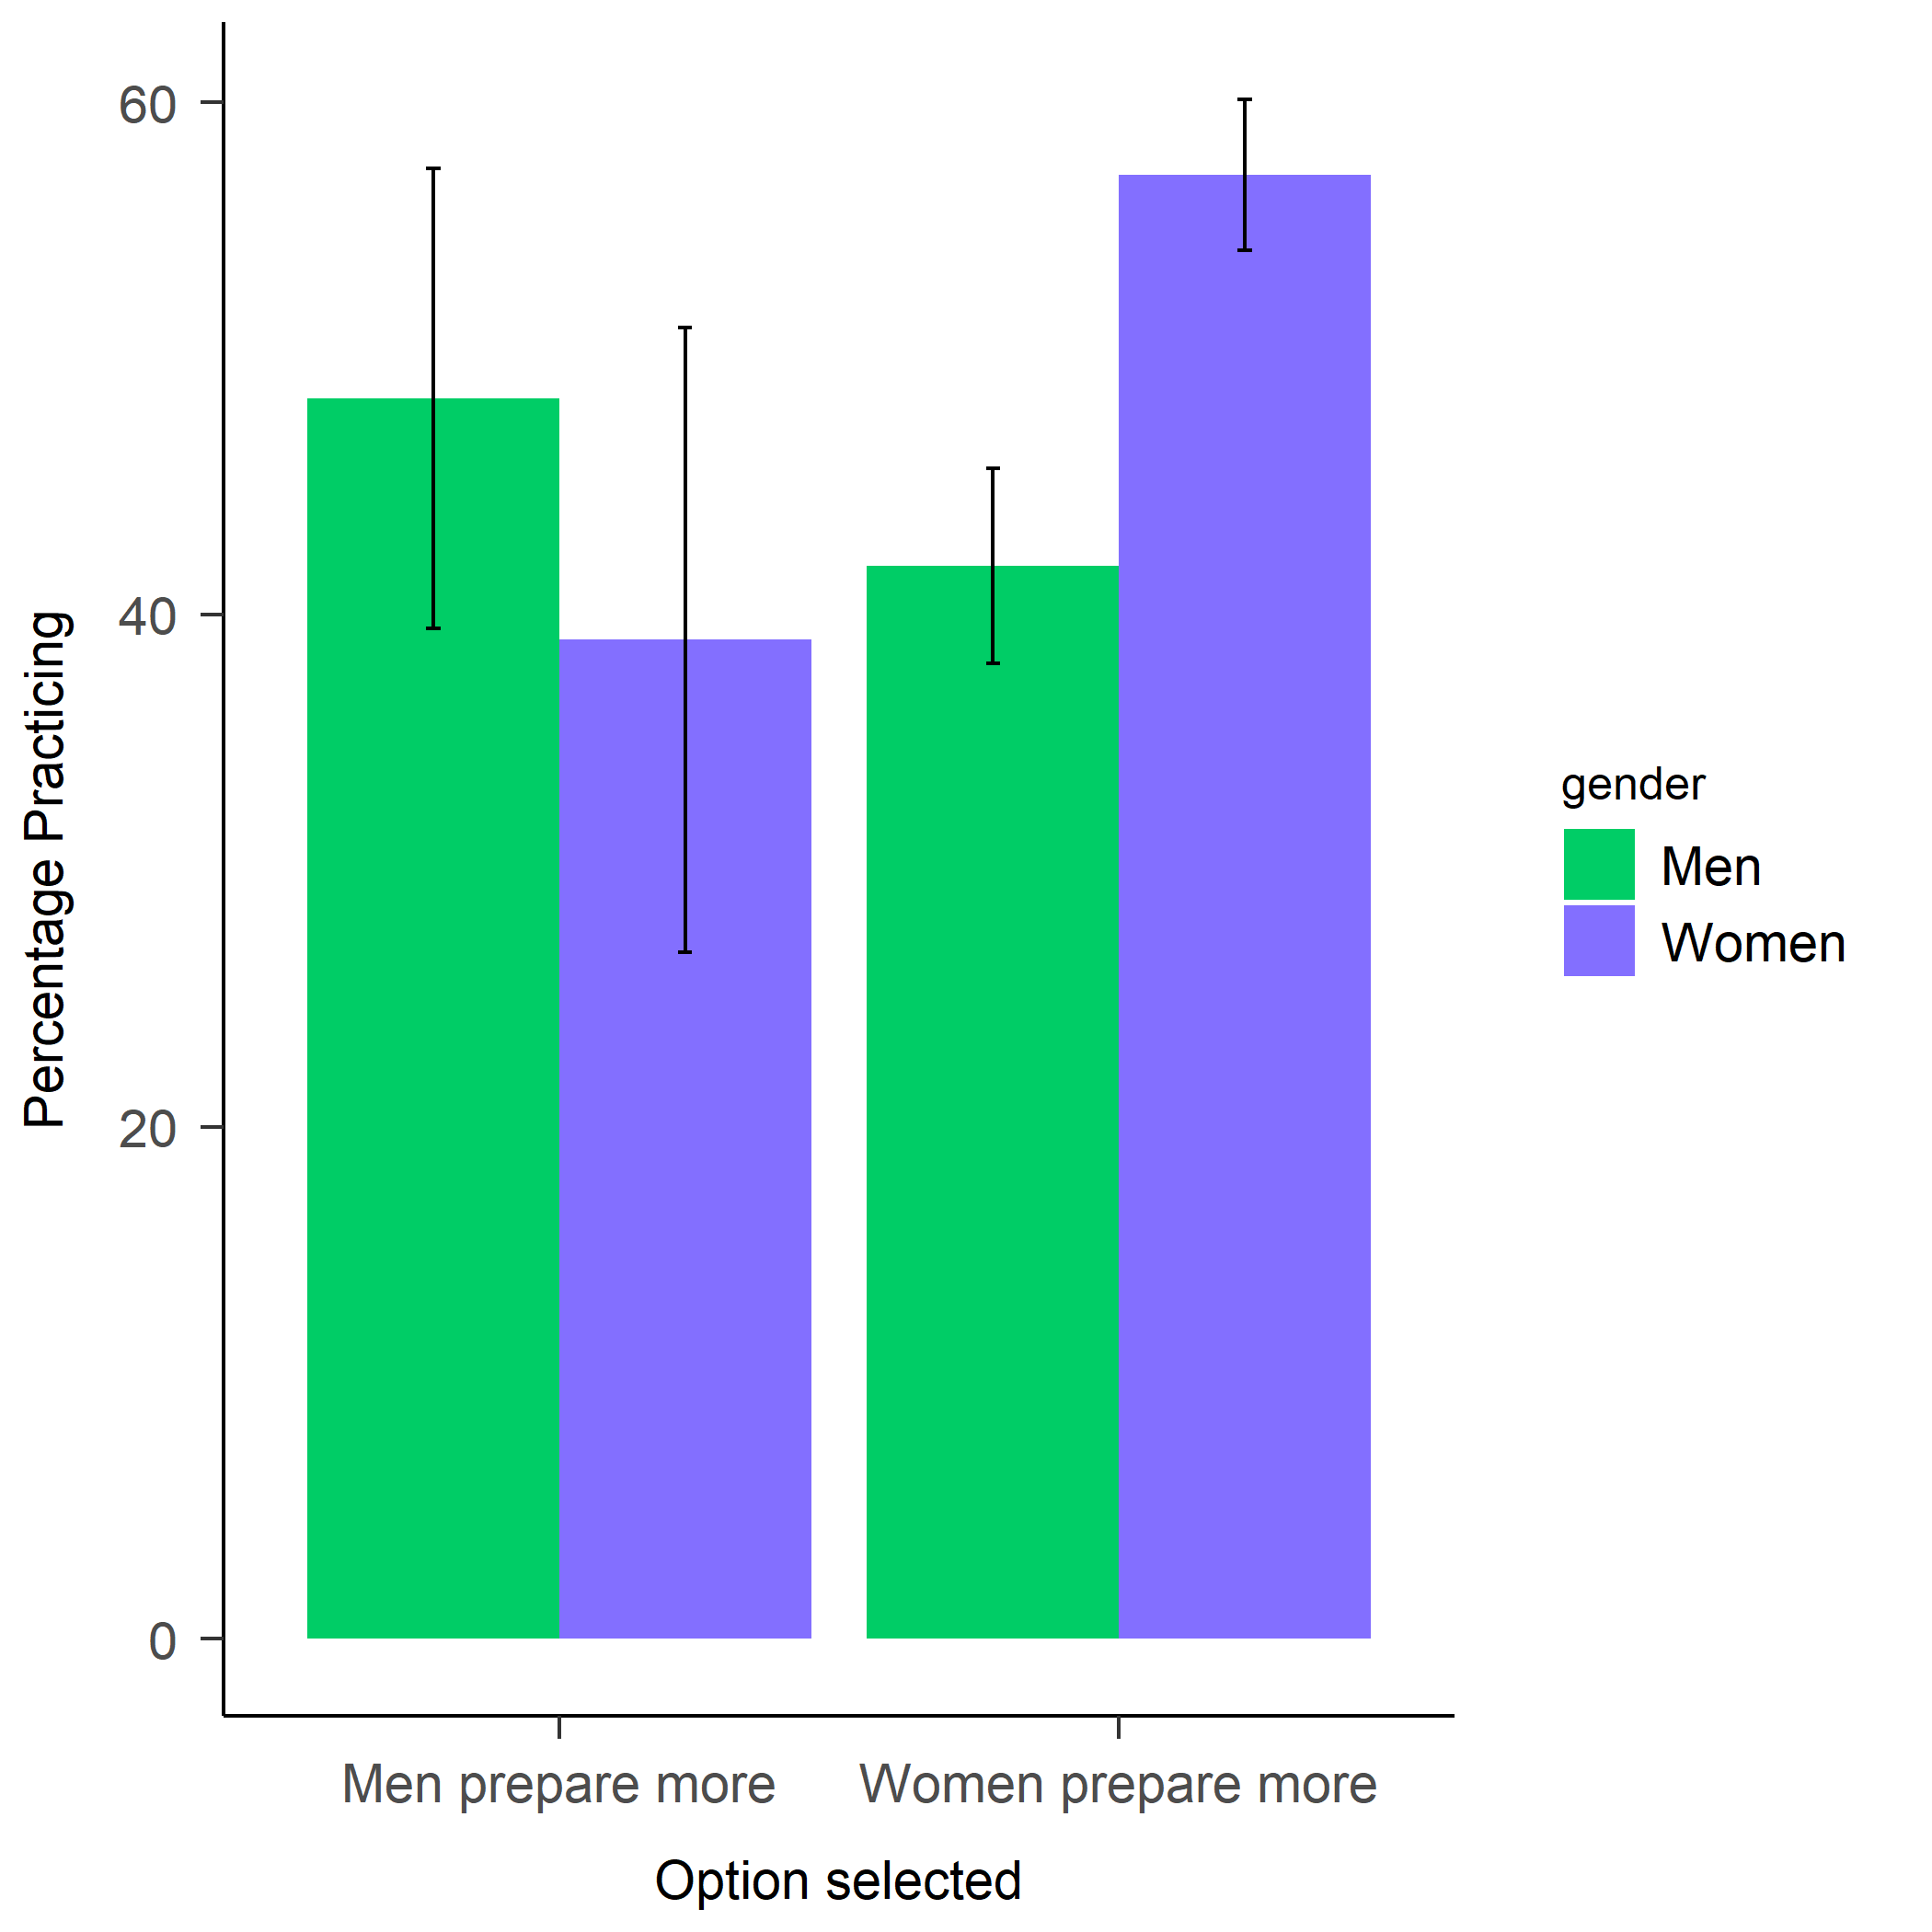
\includegraphics[width=300px]{C:/Users/keana/OneDrive - PennO365/Comp_transfer2018/Penn/practice_study/gender-practice/study1/figs/pract-choice-by-gender-and-perc-gen-prep-bar-study1} 

}

\caption{Proportion of men and women in Study 1 who chose to practice based on whether they thought men or women spend more time preparing on most tasks. Women who thought women generally prepare more were especially likely to choose to practice. Error bars represent standard errors.}\label{fig:pract-choice-by-gender-and-perc-gen-prep-bar-study1}
\end{figure}

\begin{figure}

{\centering 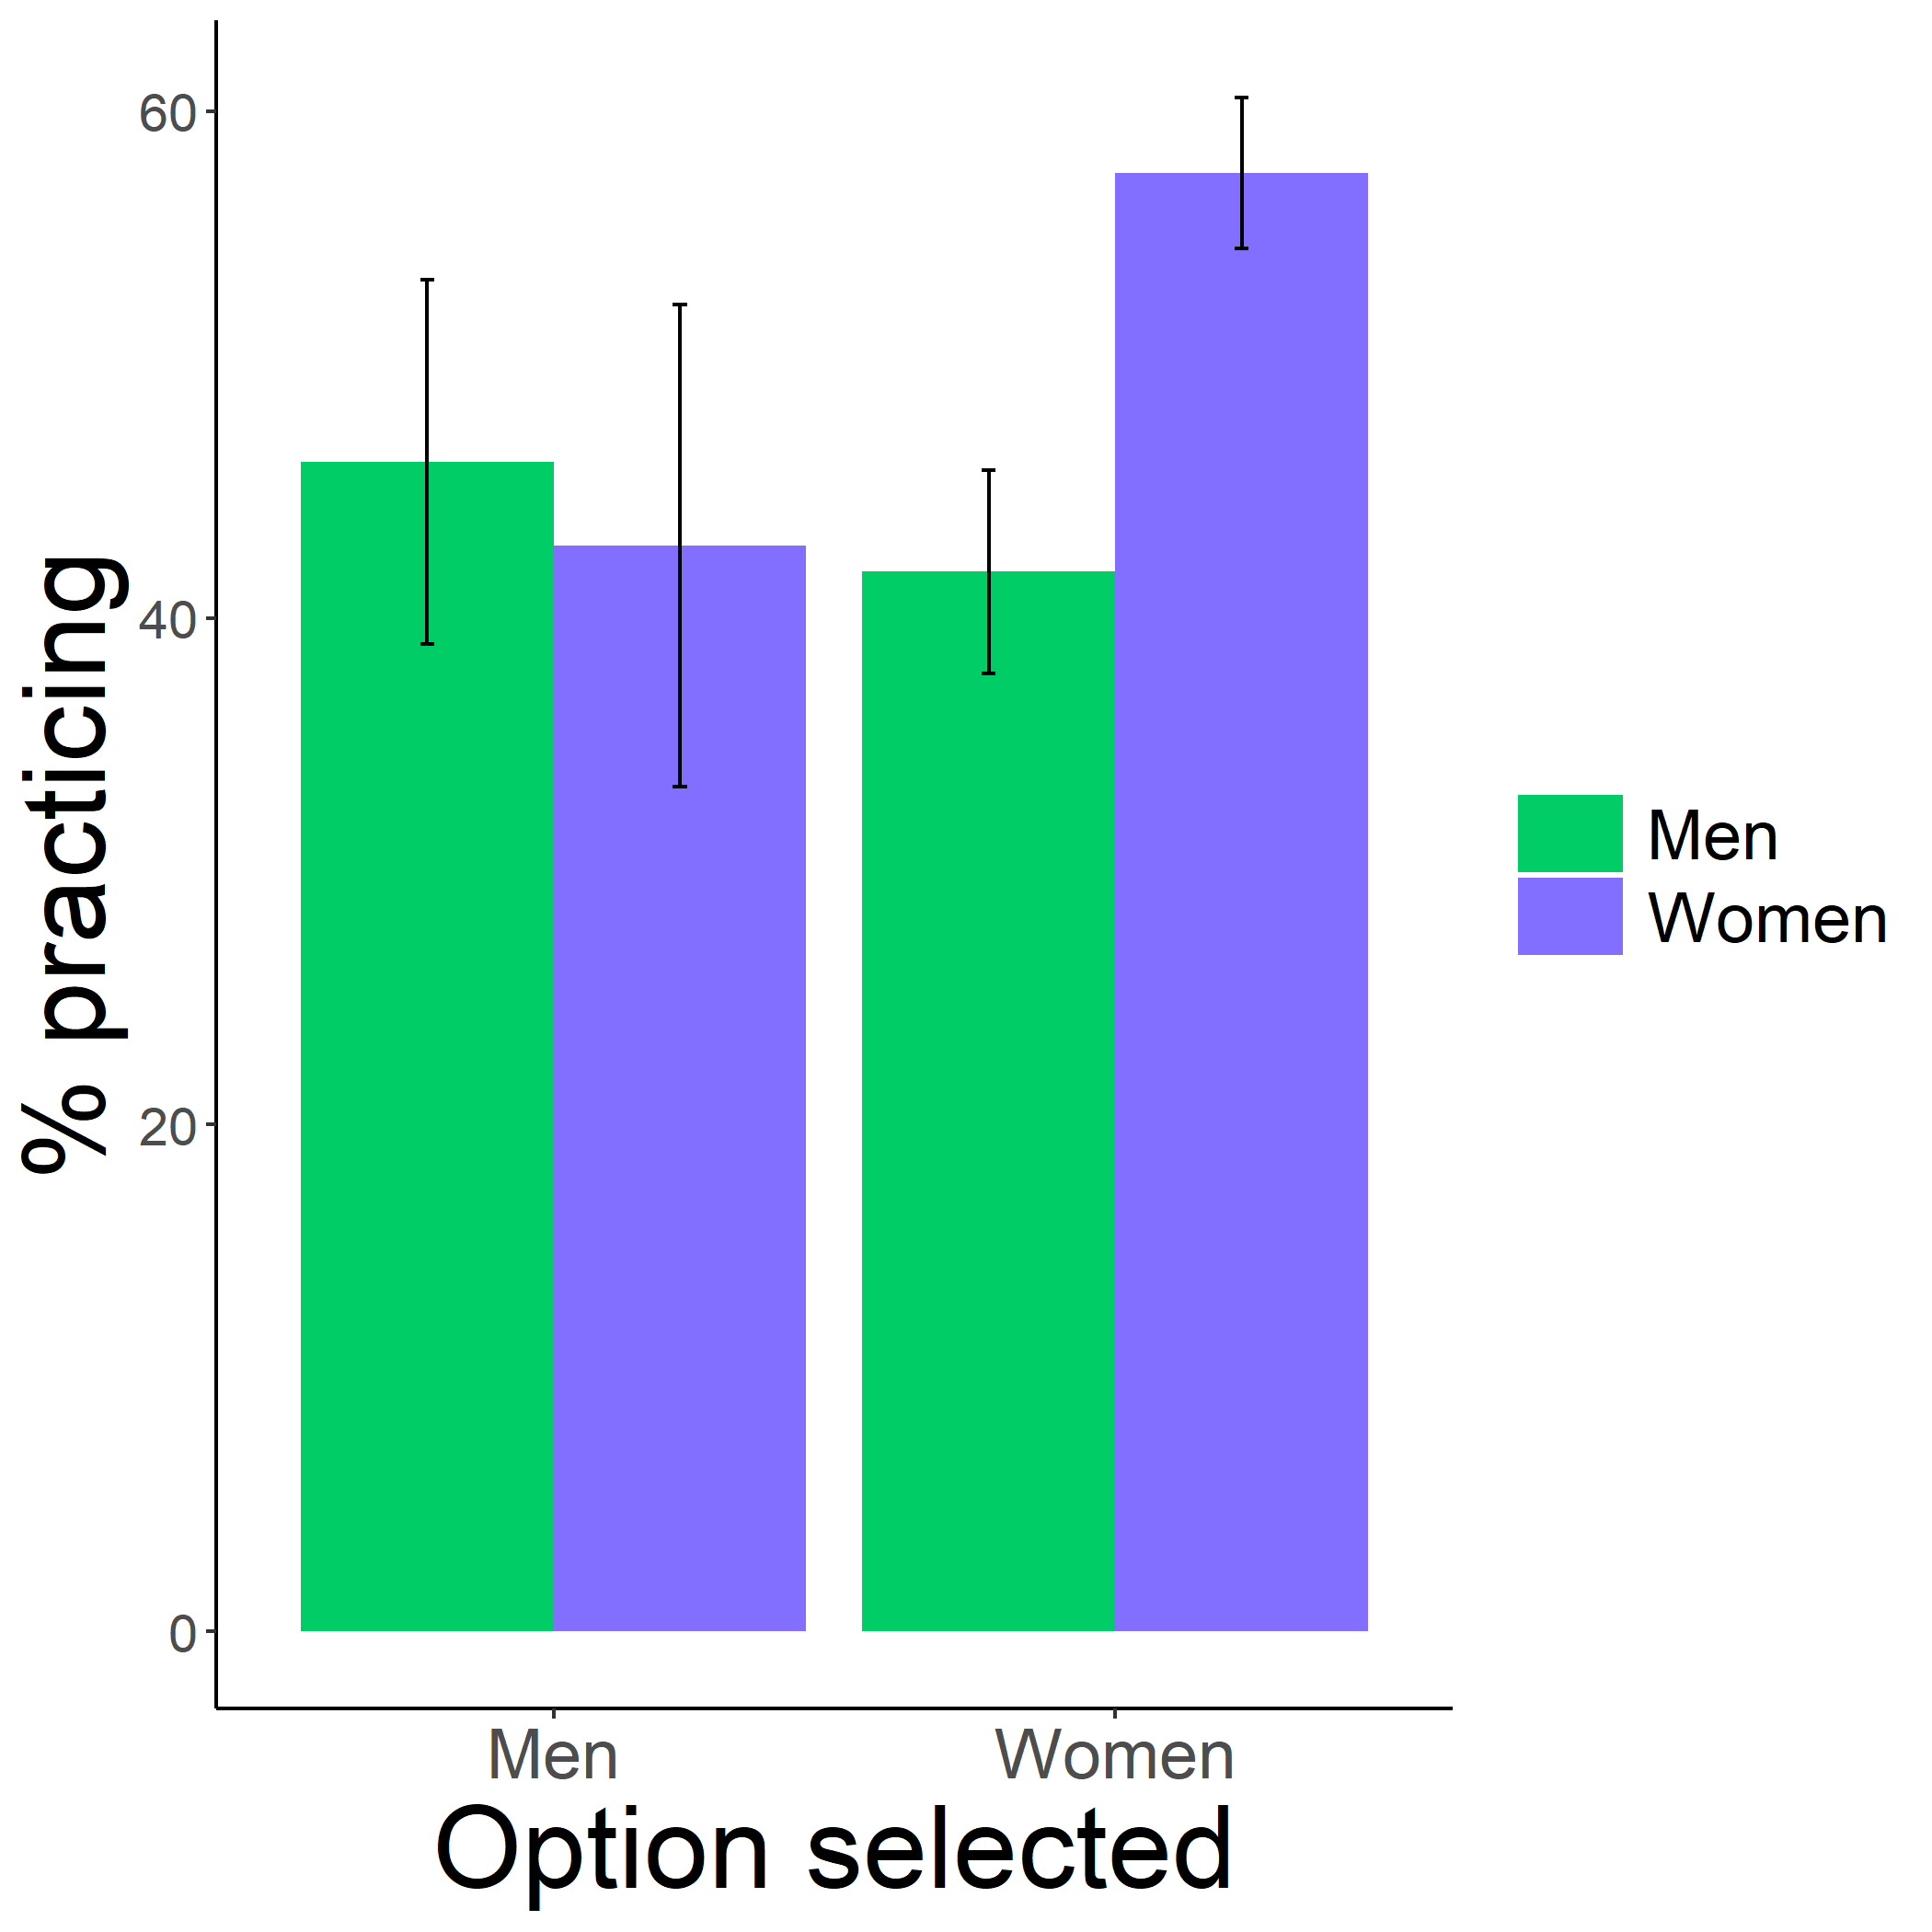
\includegraphics[width=300px]{C:/Users/keana/OneDrive - PennO365/Comp_transfer2018/Penn/practice_study/gender-practice/study1/figs/pract-choice-by-gender-and-perc-task-prep-bar-study1} 

}

\caption{Proportion of men and women in Study 1 who chose to practice based on whether they thought men or women spend more time preparing for the multiplication task. Women who thought women prepare more for the multiplication task were especially likely to choose to practice. Error bars represent standard errors.}\label{fig:pract-choice-by-gender-and-perc-task-prep-bar-study1}
\end{figure}

\hypertarget{responses-to-calculator-use-questions}{%
\subsubsection{Responses to calculator use questions}\label{responses-to-calculator-use-questions}}

Finally, we analyzed participants' responses to the questions about their calculator use and thoughts on using a calculator for the multiplication task. 86\% of participants indicated that they thought using a calculator to answer the multiplication questions would slow them down and 93\% of participants said they did not use a calculator. Importantly, there were no gender differences in perceptions of how calculators would affect performance, \(\chi^2(1, n = 1056) = 0.42\), \(p = .519\). Additionally, we did not find evidence of gender differences in actual calculator use, \(\chi^2(1, n = 1056) = 1.70\), \(p = .193\).

\hypertarget{discussion}{%
\subsection{Discussion}\label{discussion}}

\hypertarget{summary-of-main-experimental-results}{%
\subsubsection{Summary of main experimental results}\label{summary-of-main-experimental-results}}

Here we examine how knowledge of an opportunity to prepare influences gender differences in competitiveness. Our results suggest that knowledge of an opportunity to prepare did not change women and men's behavior to significantly different degrees. We also do not find evidence of any effect of condition on the choice to compete in general, such that participants' who knew they could prepare before choosing to compete were not significantly more likely to choose to compete than participants who were not provided this information before deciding whether to compete.

Despite no evidence of our anticipated effects of condition and the interaction between gender and condition on the choice to compete, we still find that men choose to compete significantly more than women, an effect that is explained by differences in risk attitudes and task scores.

Relative to other studies, only a small proportion of men (20.25\%) and women (11.19\%) in the current study chose to compete. For instance, \textcite{Niederle2007} find that 35\% of women and 73\% of men chose to compete. It is possible that the online nature of the task may have contributed to this result, which we explore further in the broader discussion section summarizing results across studies.

Contrary to previous research using similar arithmetic tasks \autocite[see review in][]{Niederle2011}, we find that gender predicts task score, over and above other possible variables that likely drive performance (e.g., risk attitudes, choice in a payment scheme, confidence). We discuss implications of this finding further in the context of the rest of the results across studies in the overall discussion section.

\hypertarget{gender-differences-in-preparation-1}{%
\subsubsection{Gender differences in preparation}\label{gender-differences-in-preparation-1}}

Based on the binary measure of preparation, we find that women choose to prepare more than men, independent of whether they had chosen the competitive tournament or non-competitive piece-rate payment scheme. However, we do not find evidence that gender predicts the number of practice rounds completed.

We also included several incentivized questions eliciting participants' beliefs about gender differences across many of our behavioral variables of interest. Both men and women were significantly more likely than chance to say that women prepare more than men both before completing the multiplication task and in general\footnote{Note that the question about general differences in practicing was unincentivized}. Though we cannot directly attest to the general accuracy of these gender differences in preparation, since there is little research that has directly tested these gender differences, our study shows that women do indeed choose to prepare more than men, regardless of the payment scheme that they chose for their performance. Thus, we have our first piece of evidence from this study that gender differences in the choice to prepare and gender stereotypes about preparation are aligned. This alignment suggests that gender stereotypes about practicing exist among the general population represented by our sample and may, at least for the task used in the current study, be accurate. Of course, these beliefs were elicited after participants themselves chose whether or not to practice. As such, their answers may have been influenced by knowledge of their own gender and behavior in the study and may not be reflective of strong gender stereotypes. Future work should explore participants' how beliefs may be shaped by the decision making-process and/or elicit beliefs before participants make any decisions to practice.

\hypertarget{perceptions-of-gender-differences-in-preparation-performance-and-competitiveness-1}{%
\subsubsection{Perceptions of gender differences in preparation, performance, and competitiveness}\label{perceptions-of-gender-differences-in-preparation-performance-and-competitiveness-1}}

Also, both men and women were significantly more likely than chance to correctly state that men would be more likely to choose to compete during the multiplication task, suggesting strong stereotypes about gender differences in competitiveness that align with observed behavior across the literature. The finding that participants believe women compete less suggests that they did not believe women prepare more because they were more likely to compete and used preparation as a way to increase the probability that they would earn more during the competition.

One possible explanation for participants' predictions is that they expected men to outperform women on the task, which would lead women to compensate by preparing more. Yet, they don't expect that: participants were equally likely to predict that women (vs.~men) would perform better on the task, suggesting that participants did not have strong stereotypes about gender differences in performance on the multiplication task.

\hypertarget{effects-of-gender-and-perceptions-on-practicing-1}{%
\subsubsection{Effects of gender and perceptions on practicing}\label{effects-of-gender-and-perceptions-on-practicing-1}}

On top of the gender differences in practicing and perceptions of said gender differences, we explored whether these perceptions are aligned with individuals' practicing behavior. More specifically, we would expect that women may be especially likely to prepare for the task if they believe that women will prepare more than men, both in general on most tasks and specifically within the context of the multiplication task. We find support for this hypothesis across both questions about perceptions of gender differences in preparation. Though we cannot test this hypothesis causally with this specific set of data, these results would suggest that women's practicing behavior may have been influenced at least in part by beliefs about gender differences in preparation (though see Overall Discussion section for considerations of this interpretation).

\hypertarget{self-reported-calculator-use-and-perceptions-of-calculator-use}{%
\subsubsection{Self-reported calculator use and perceptions of calculator use}\label{self-reported-calculator-use-and-perceptions-of-calculator-use}}

There may be concern that participants used a calculator to answer the multiplication questions, which could affect the interpretation of the results if there is a gender difference in calculator use and/or calculator use is related to the choice to prepare. To address that potential concern, we included questions about participants' perceptions of and actual behaviors when it came to using calculators on the paid multiplication task. Based on their responses, it is unlikely that participants used calculators in the first place. We found that participants were unlikely to use calculators to complete the task and more importantly, there were no gender differences in the choice to use a calculator. Overall, we do not have evidence that gender differences in calculator use will be a confound when interpreting our results.

\hypertarget{summary}{%
\subsubsection{Summary}\label{summary}}

Overall, we find from the first study of Chapter 1 that our manipulation of the knowledge of the opportunity to prepare did not reduce the gender difference in competitiveness. We show that the gender difference in competitiveness itself is explained by gender differences in risk attitudes and task scores. Although the manipulation did not have the anticipated effects on gender differences in competitiveness, women chose to prepare more than men, which aligned with beliefs about gender differences in preparation. We also have evidence that women's preparation behaviors may in fact have been influenced by beliefs about gender differences in preparation. Finally, we show that participants were unlikely to be using calculators while completing the task, so it is unlikely that any of the effects found are confounded by participants' calculator use. Since we did not find evidence that the knowledge of the opportunity to prepare affected gender differences in competitiveness, the next study in Chapter 1 tests experimentally whether the actual experience of preparing through required preparation for a pre-specified number of rounds would affect the gender gap in competitiveness. We expect individuals may need to actually experience improvement in their performance directly for the preparation to affect one's willingness to compete.

\newpage

\hypertarget{study-2}{%
\section{Study 2}\label{study-2}}

\hypertarget{methods-1}{%
\subsection{Methods}\label{methods-1}}

\hypertarget{participants-1}{%
\subsubsection{Participants}\label{participants-1}}

All study measures described below are publicly available on OSF both as a \href{https://osf.io/9pt2e/}{.pdf} and \href{https://osf.io/bxwu2/}{.qsf}. Participants were recruited on Amazon Mechanical Turk via CloudResearch using the same screening criteria as Study 1. For all studies in the dissertation after Study 1 of Chapter 1, we used CloudResearch to filter out participants that had already participated in any of the other studies in this dissertation. Therefore, only MTurkers who were naive to the design were included in the current and subsequent studies. Also, if participants had an identical IP address, MTurkID, and gender, we excluded their second response. The final sample consisted of 1088 participants (50.64\% women), with an average age of 38.54 (\emph{SD} = 12.5) years. 62 participants (51.61\% women) dropped out of the study before finishing\footnote{Note: we use data from participants who dropped out when available}.

\newpage

\begin{center}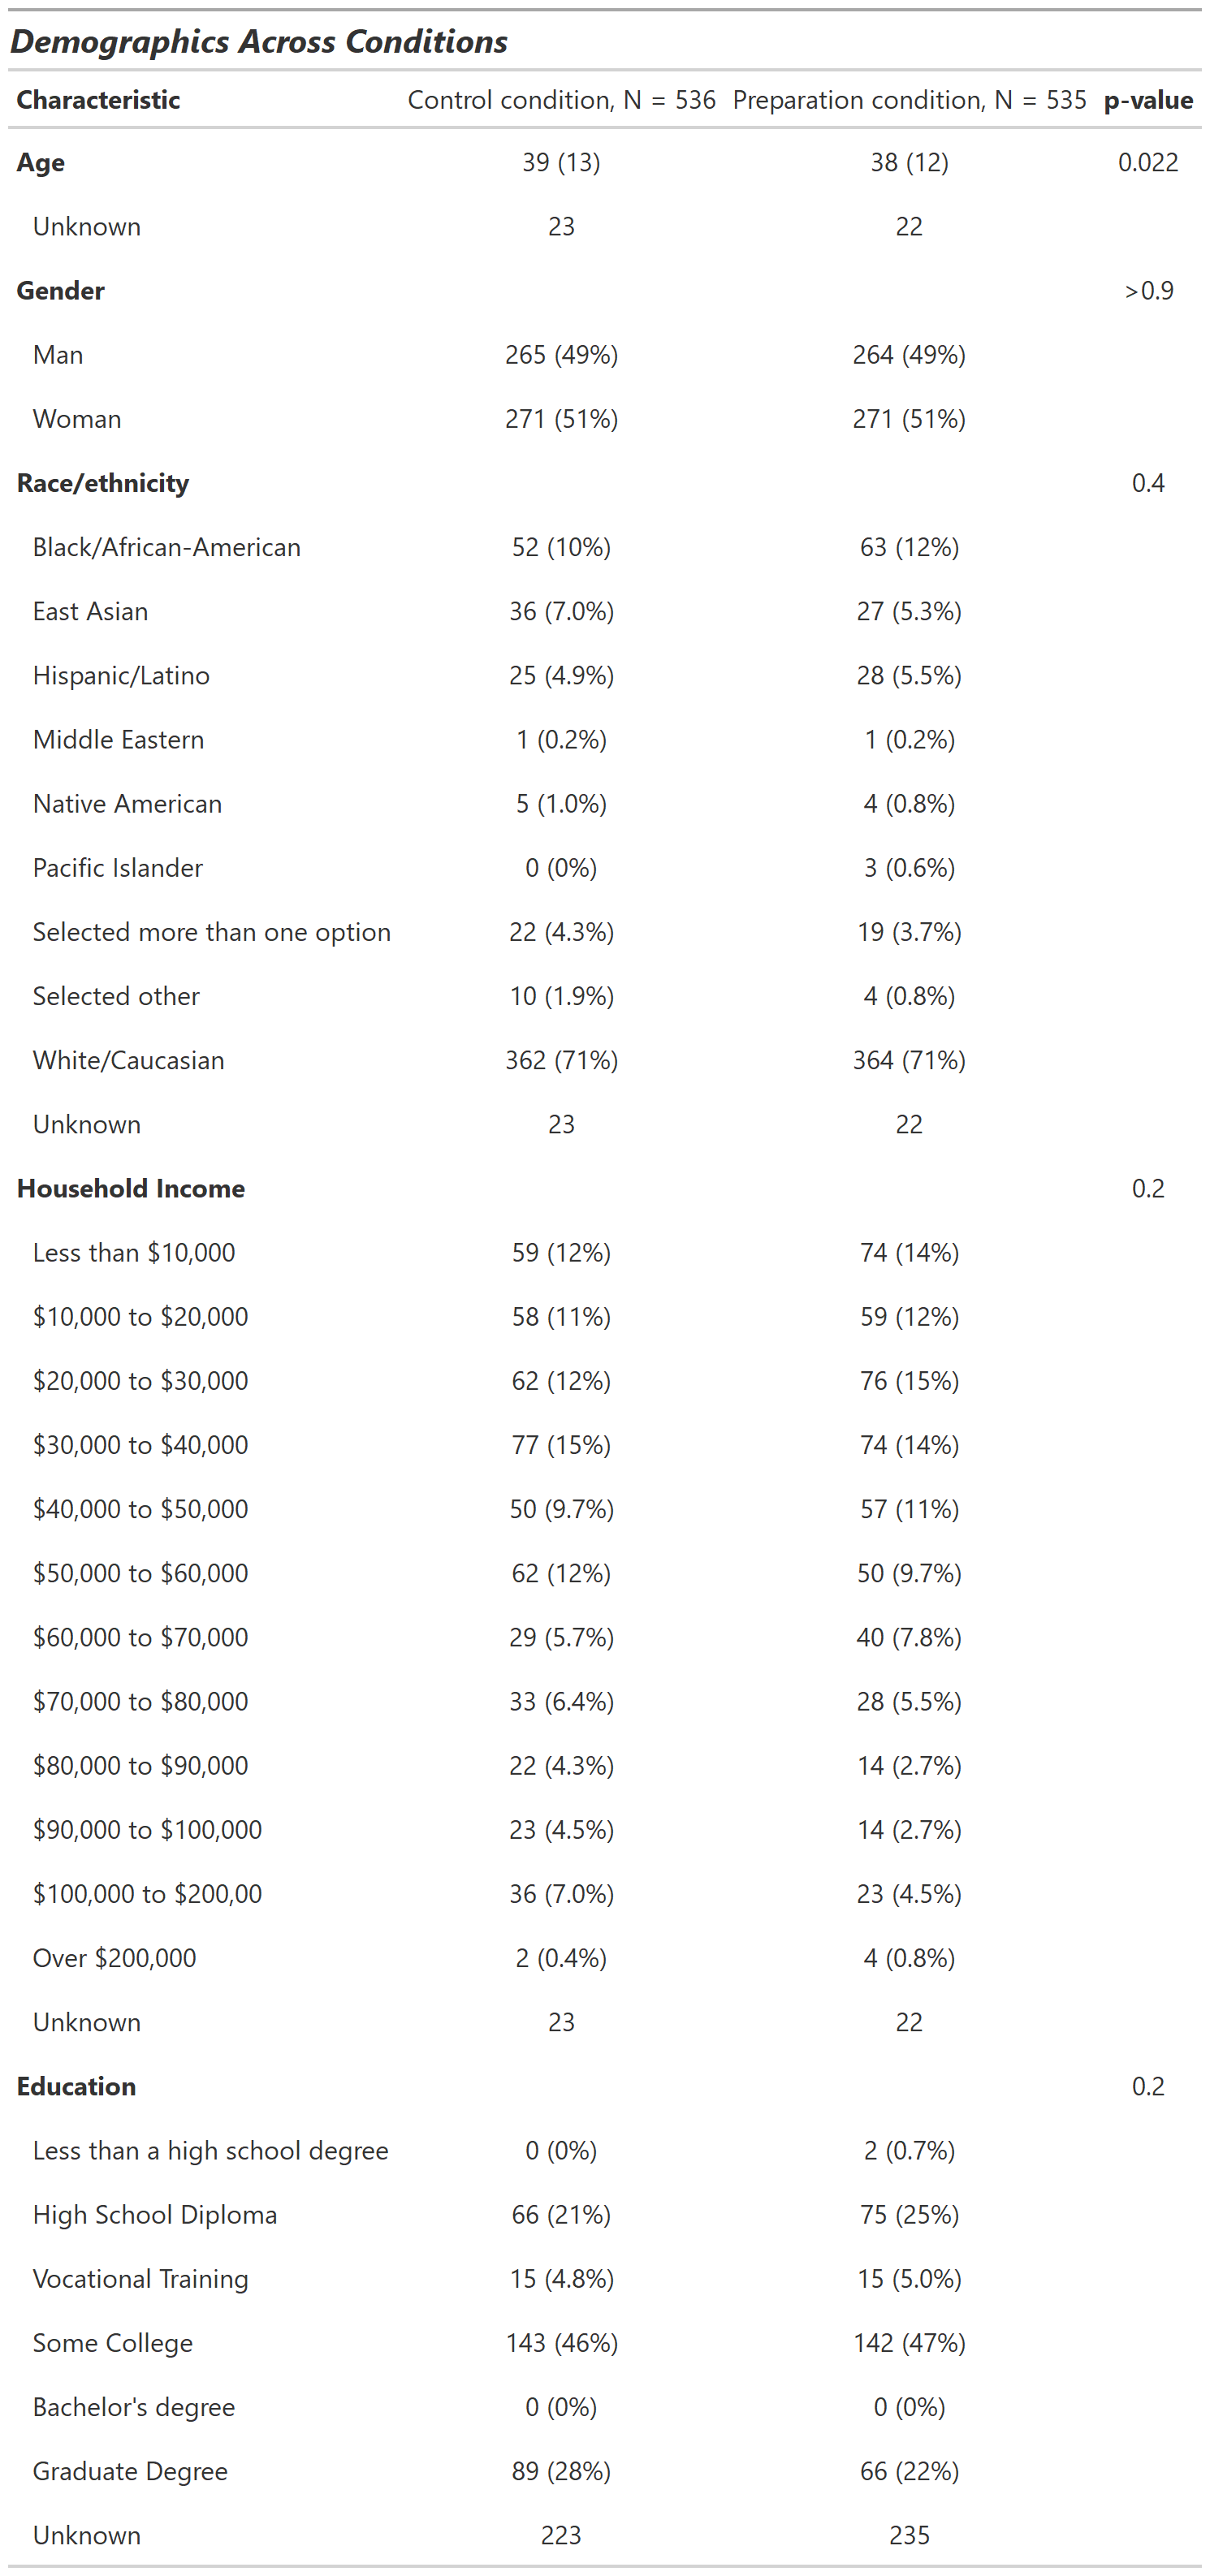
\includegraphics[width=0.6\linewidth]{C:/Users/keana/OneDrive - PennO365/Comp_transfer2018/Penn/practice_study/gender-practice/study2/figs/demographics-table-conds-study2} \end{center}

\begin{table}[ht]
\centering
\begingroup\fontsize{0.1pt}{0.1pt}\selectfont
\begin{tabular}{r}
   \\ 
 \end{tabular}
\endgroup
\caption{Size of sample in Study 2 with corresponding percentage listed for gender, race, education, and household income, with p-values derived from Fisher’s exact test. Mean with corresponding standard deviation listed for age, with p-values derived from Kruskal-Wallis test. If a participant did not respond to a given question, we list their response as ‘Unknown’.} 
\label{tab:demographics-table-study2}
\end{table}

\newpage

\begin{center}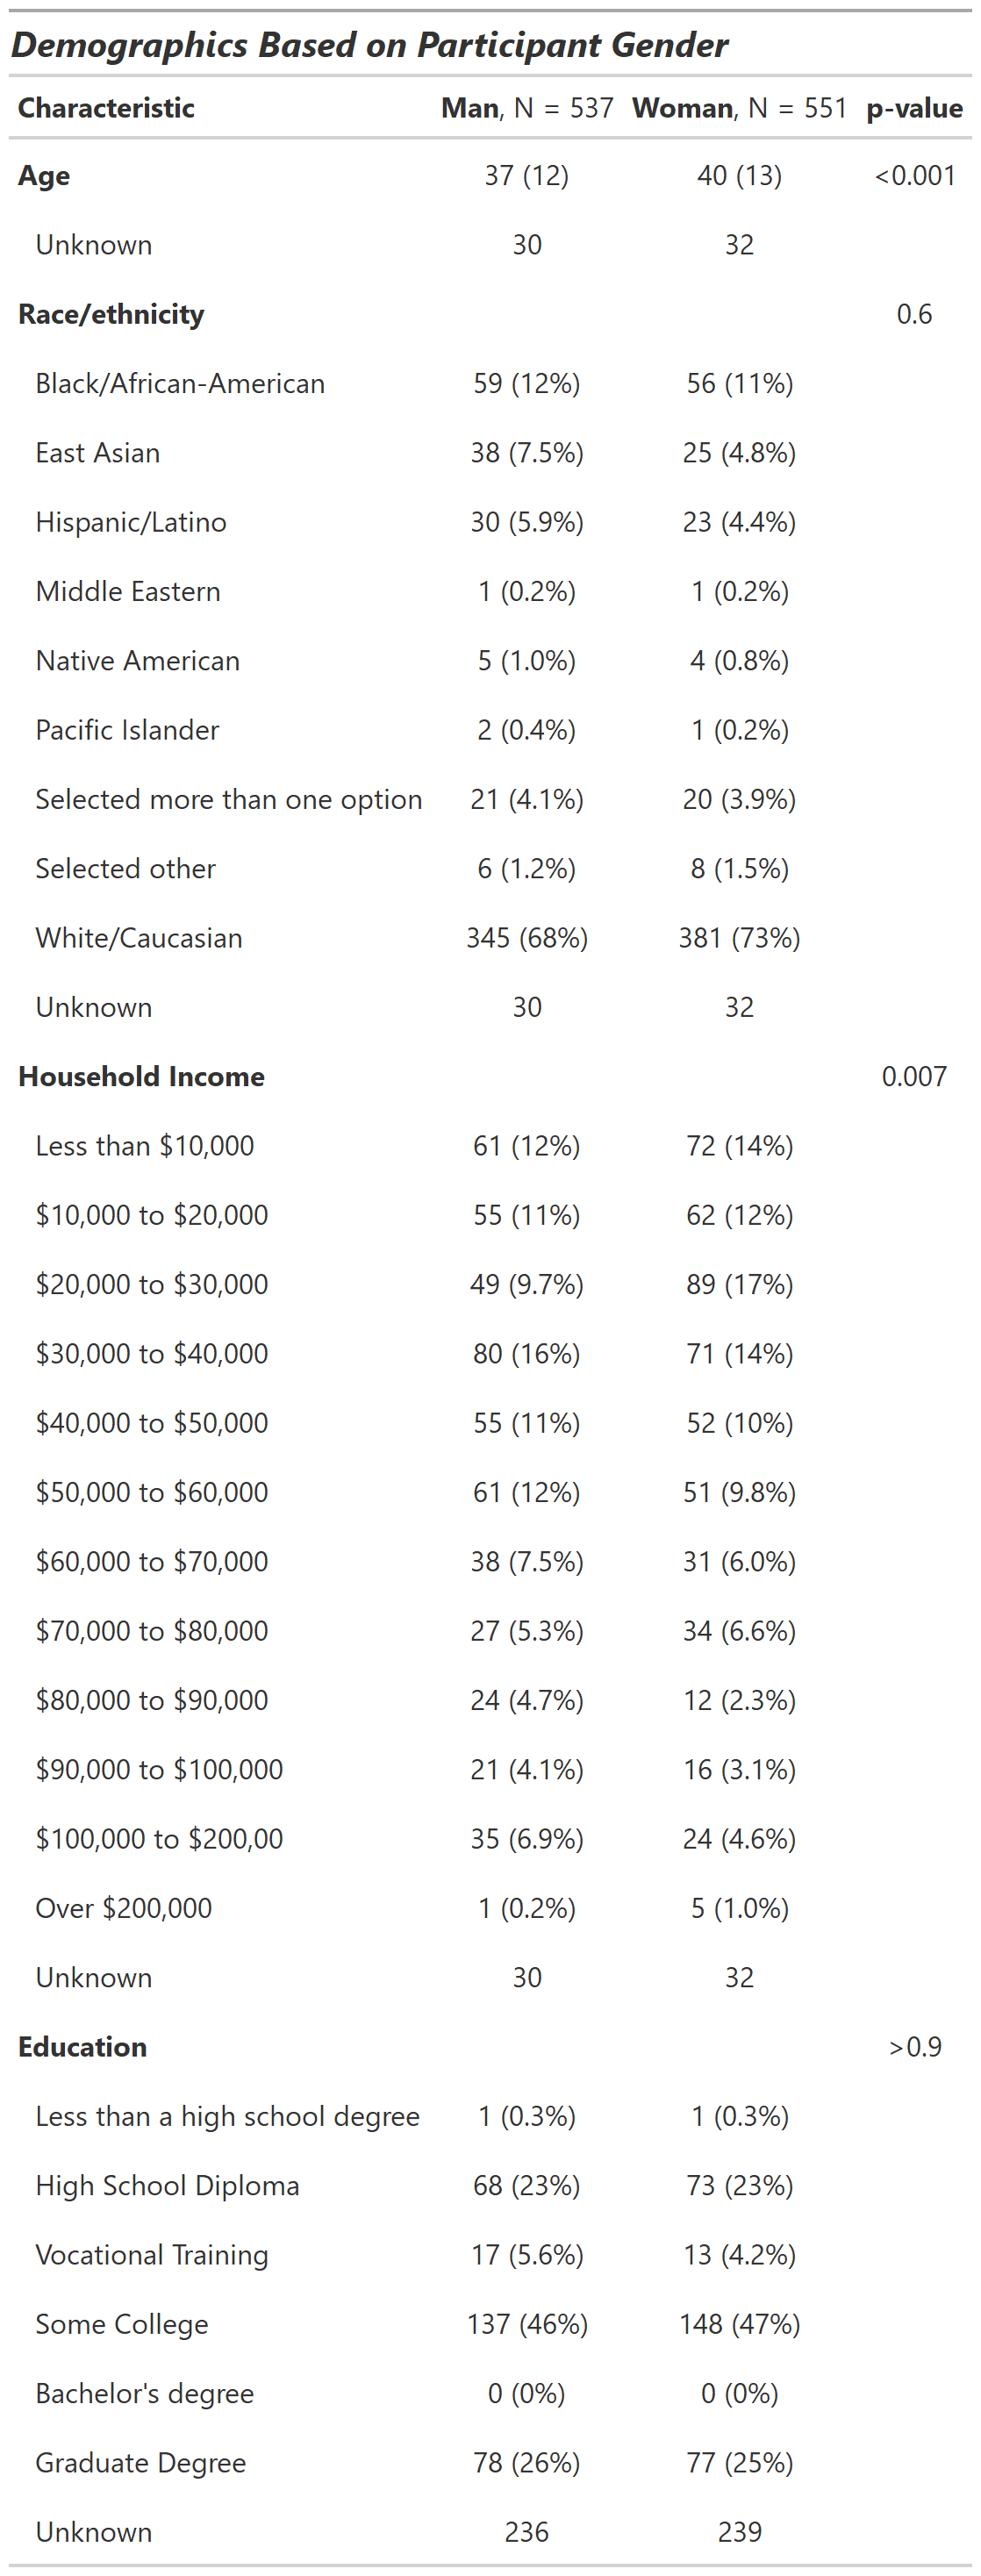
\includegraphics[width=0.5\linewidth]{C:/Users/keana/OneDrive - PennO365/Comp_transfer2018/Penn/practice_study/gender-practice/study2/figs/demographics-table-gender-study2} \end{center}

\begin{table}[ht]
\centering
\begingroup\fontsize{0.1pt}{0.1pt}\selectfont
\begin{tabular}{r}
   \\ 
 \end{tabular}
\endgroup
\caption{Size of sample in Study 2 with corresponding percentage listed for race, education, and household income, with p-values derived from Fisher’s exact test. Mean with corresponding standard deviation listed for age, with p-values derived from Kruskal-Wallis test. If a participant did not respond to a given question, we list their response as ‘Unknown’.} 
\label{tab:demographics-table-gender-study2}
\end{table}

\hypertarget{procedures-1}{%
\subsubsection{Procedures}\label{procedures-1}}

As in Study 1, participants included in the study were told they would be completing a two-minute multiplication task (identical to the one used in Study 1) and would be able to choose a payment scheme for their performance. The instructions and payment per question were identical to Study 1. After being told about the rules for the multiplication task and passing the same comprehension questions used in Study 1, participants were randomly assigned to either a preparation condition, where they were told they would complete several rounds of preparation before completing the multiplication task, or a control condition, where they were told they would complete several rounds of a counting task before continuing. Participants were randomly assigned to each condition, control= 50.05\%. Of the men who completed the study, 50.09\% were assigned to the control condition and of the women who completed the study, 50\% were assigned to the control condition, \(\chi^2(1, n = 1088) = 0.00\), \(p > .999\).

The participants in the preparation condition completed 12 rounds of practice for each multiplication table (i.e., tables 1-12), with 6 problems per round. The problems for each round were selected at random. Participants in the control condition were asked to complete 5 questions where they counted the number of zeros in a 7x7 matrix of zeros and ones. After a 30-second break following completion of their respective tasks, all participants chose a payment scheme (i.e., piece-rate or tournament) for the multiplication task, where the order of presentation was counterbalanced. That is, half of the participants saw the tournament scheme presented as the first option and half saw the piece-rate payment scheme presented first.

After choosing a payment scheme, participants in both conditions had the option to spend (extra) time preparing for the multiplication task. Importantly, they were not told about the additional opportunity to prepare until after they made their decision to compete. Again, we had two measures of preparation behavior: the binary decision to practice and the number of extra practice rounds completed. If they chose to prepare, participants were given two minutes to complete a randomly selected set of problems from all 12 multiplication tables. Once they finished the first two-minute preparation round, participants could opt into 4 more rounds of preparation, each two minutes long, before they moved on to the paid portion of the study. Here, the practice rounds variable is encoded the same way for participants across conditions, where the choice to practice is encoded as 1 for that variable, and the variable increases incrementally (up to 5 given the design) thereafter (\emph{M} = 0.53, \emph{SD} = 0.82); 39.04\% of participants opted for additional practice.

Then, participants completed the paid multiplication task for two minutes. We included many of the same follow-up questions as in Study 1, including risk aversion, confidence, and perceptions of gender differences in preparation, competitiveness, and performance. Like Study 1, participants were incentivized to answer the questions about their confidence and perceptions of gender differences correctly. Specifically, they were told that one of their responses to those questions would be randomly selected and if the selected option was correct, they would earn a bonus of \$.10 on top of their guaranteed earnings. We also asked participants if they wished they had more time to prepare for the multiplication task, a binary variable (response options: ``Yes'' or ``No'') that we subsequently describe as participants' self-reported ``feelings of preparedness''. Thereafter, we included measures of their fatigue, field-specific ability beliefs, and interest in the multiplication task all on 1 (Strongly disagree) to 7 (Strongly agree) scales. For the fatigue scale, participants rated how fatigued and mentally exhausted they felt \autocite{Milyavskaya2018}. Participants indicated the degree to which they ``enjoyed completing the multiplication task'' for the interest scale \autocite{Milyavskaya2018}. Finally, to measure field-specific ability beliefs, we asked participants how much they perceived success in math depends on ability versus effort through six questions (e.g., ``If you want to succeed in math, hard work alone just won't cut it; you need to have an innate gift or talent'') \autocite{Meyer2015}.

\hypertarget{results-1}{%
\subsection{Results}\label{results-1}}

\hypertarget{describing-main-variables-of-interest-1}{%
\subsubsection{Describing main variables of interest}\label{describing-main-variables-of-interest-1}}

We replicated the effect of gender on the choice to compete when gender is included as the only predictor in the logistic regression: 19.85\% of men chose to compete compared to 13.91\% of women, \(b = -0.43\), 95\% CI \([-0.76\), \(-0.10]\), \(z = -2.56\), \(p = .010\). Like Study 1, the gender effect on competitiveness is no longer significant after adding the same control variables as before (i.e., risk attitudes, confidence, task scores, and the hypothesized interaction between gender and competition choice), where risk attitudes, \(b = 0.34\), 95\% CI \([0.26\), \(0.42]\), \(z = 8.34\), \(p < .001\), confidence, \(b = 0.01\), 95\% CI \([0.01\), \(0.02]\), \(z = 3.04\), \(p = .002\), and task scores, \(b = 0.01\), 95\% CI \([0.00\), \(0.02]\), \(z = 3.10\), \(p = .002\) appear to explain the gender differences in competitiveness (see Table \ref{tab:tab-comp-choice-study2}).

\begin{center}
\includegraphics[width=1\linewidth]{C:/Users/keana/OneDrive - PennO365/Comp_transfer2018/Penn/practice_study/gender-practice/study2/figs/tab_comp-choice-study2} \end{center}

\begin{table}[ht]
\centering
\begingroup\fontsize{0.1pt}{0.1pt}\selectfont
\begin{tabular}{r}
   \\ 
 \end{tabular}
\endgroup
\caption{All models are logistic regressions with choice to compete as the dependent variable, where man and control are the reference categories for participant gender and preparation condition, respectively. The gender difference in the choice to compete is not reduced by preparation condition, but is explained by risk attitudes, task scores, and confidence. p < .05 is considered significant and bolded.} 
\label{tab:tab-comp-choice-study2}
\end{table}

Again, we find that gender predicts task scores when included by itself as a predictor, \(b = -3.68\), 95\% CI \([-6.27\), \(-1.10]\), \(t(1028) = -2.80\), \(p = .005\). However, unlike Study 1, when other variables are included as predictors in the linear regression, we find that the effect of gender on task scores dissipates, \(b = -0.46\), 95\% CI \([-3.17\), \(2.24]\), \(t(1020) = -0.34\), \(p = .738\), suggesting that the other variables, such as competition choice, \(b = 7.17\), 95\% CI \([2.83\), \(11.52]\), \(t(1020) = 3.24\), \(p = .001\), risk attitudes, \(b = -1.35\), 95\% CI \([-1.85\), \(-0.86]\), \(t(1020) = -5.42\), \(p < .001\), and confidence, \(b = 0.35\), 95\% CI \([0.30\), \(0.41]\), \(t(1020) = 12.54\), \(p < .001\), explained the gender difference in task scores in this study (see \ref{tab:tab-task-scores-study2}). In support of this possibility, we replicate the finding from the Study 1 of this chapter that gender predicts both risk attitudes, \(b = -1.14\), 95\% CI \([-1.46\), \(-0.82]\), \(t(1024) = -7.00\), \(p < .001\) and confidence, \(b = -9.76\), 95\% CI \([-12.49\), \(-7.02]\), \(t(1027) = -6.99\), \(p < .001\). See Table \ref{tab:summary-table-gender-study2} for a summary of gender differences in the main variables of interest.

\begin{center}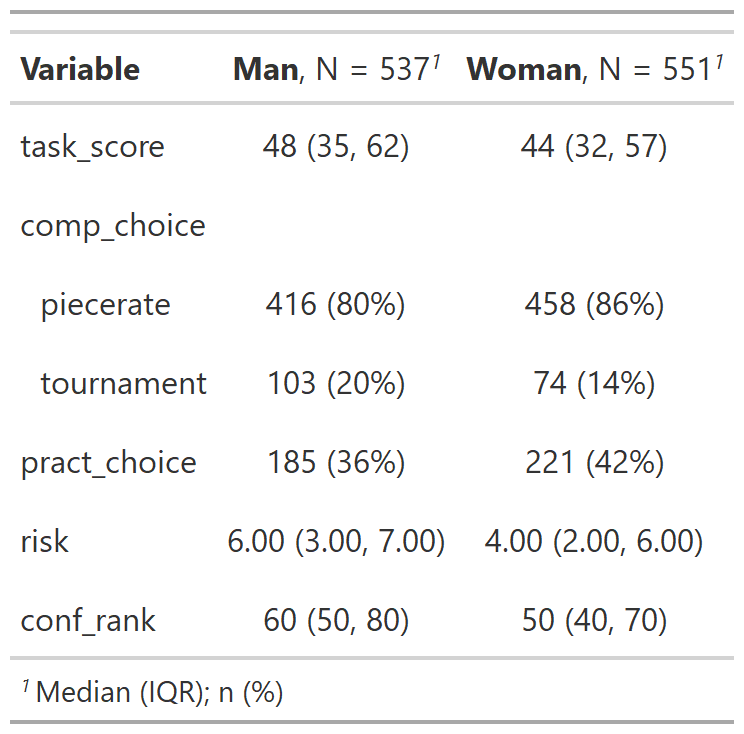
\includegraphics[width=0.5\linewidth]{C:/Users/keana/OneDrive - PennO365/Comp_transfer2018/Penn/practice_study/gender-practice/study2/figs/summary-table-gender-study2} \end{center}

\begin{table}[ht]
\centering
\begingroup\fontsize{0.1pt}{0.1pt}\selectfont
\begin{tabular}{r}
   \\ 
 \end{tabular}
\endgroup
\caption{Gender differences in the main variables of interest, including: task scores, choice to compete, choice to practice, confidence, and risk attitudes. Medians are reported for task score, risk attitudes, and confidence, with IQRs in parentheses. For choice to practice and choice to compete, we report the number and percentage of participants that fall into each category for each respective gender.} 
\label{tab:summary-table-gender-study2}
\end{table}

\newpage

\begin{center}
\includegraphics[width=1\linewidth]{C:/Users/keana/OneDrive - PennO365/Comp_transfer2018/Penn/practice_study/gender-practice/study2/figs/tab_task-scores-study2} \end{center}

\begin{table}[ht]
\centering
\begingroup\fontsize{0.1pt}{0.1pt}\selectfont
\begin{tabular}{r}
   \\ 
 \end{tabular}
\endgroup
\caption{All models are linear regressions with task score as the dependent variable, where man and piece-rate payment scheme are the reference categories for participant gender and competition choice, respectively. After controlling for risk attitudes, confidence, and competition choice, women no longer have lower scores on the multiplication task than men, p < .05 is considered significant and bolded.} 
\label{tab:tab-task-scores-study2}
\end{table}

\hypertarget{effects-of-limited-preparation-condition-on-gender-differences-in-choice-to-compete}{%
\subsubsection{Effects of limited preparation condition on gender differences in choice to compete}\label{effects-of-limited-preparation-condition-on-gender-differences-in-choice-to-compete}}

We did not find evidence of an interaction between gender and preparation condition on the choice to compete in a logistic regression, \(b = -0.17\), 95\% CI \([-0.83\), \(0.48]\), \(z = -0.51\), \(p = .610\) (see Figure \ref{fig:s200}). Also, we did not find evidence of a significant effect of condition on the choice to compete as a sole predictor in a logistic regression, \(b = -0.19\), 95\% CI \([-0.52\), \(0.13]\), \(z = -1.17\), \(p = .243\). The point estimate for the effect of the limited preparation condition was negative and the 95\% CI did not include positive effects that were greater in magnitude than 0.13.

\begin{figure}

{\centering 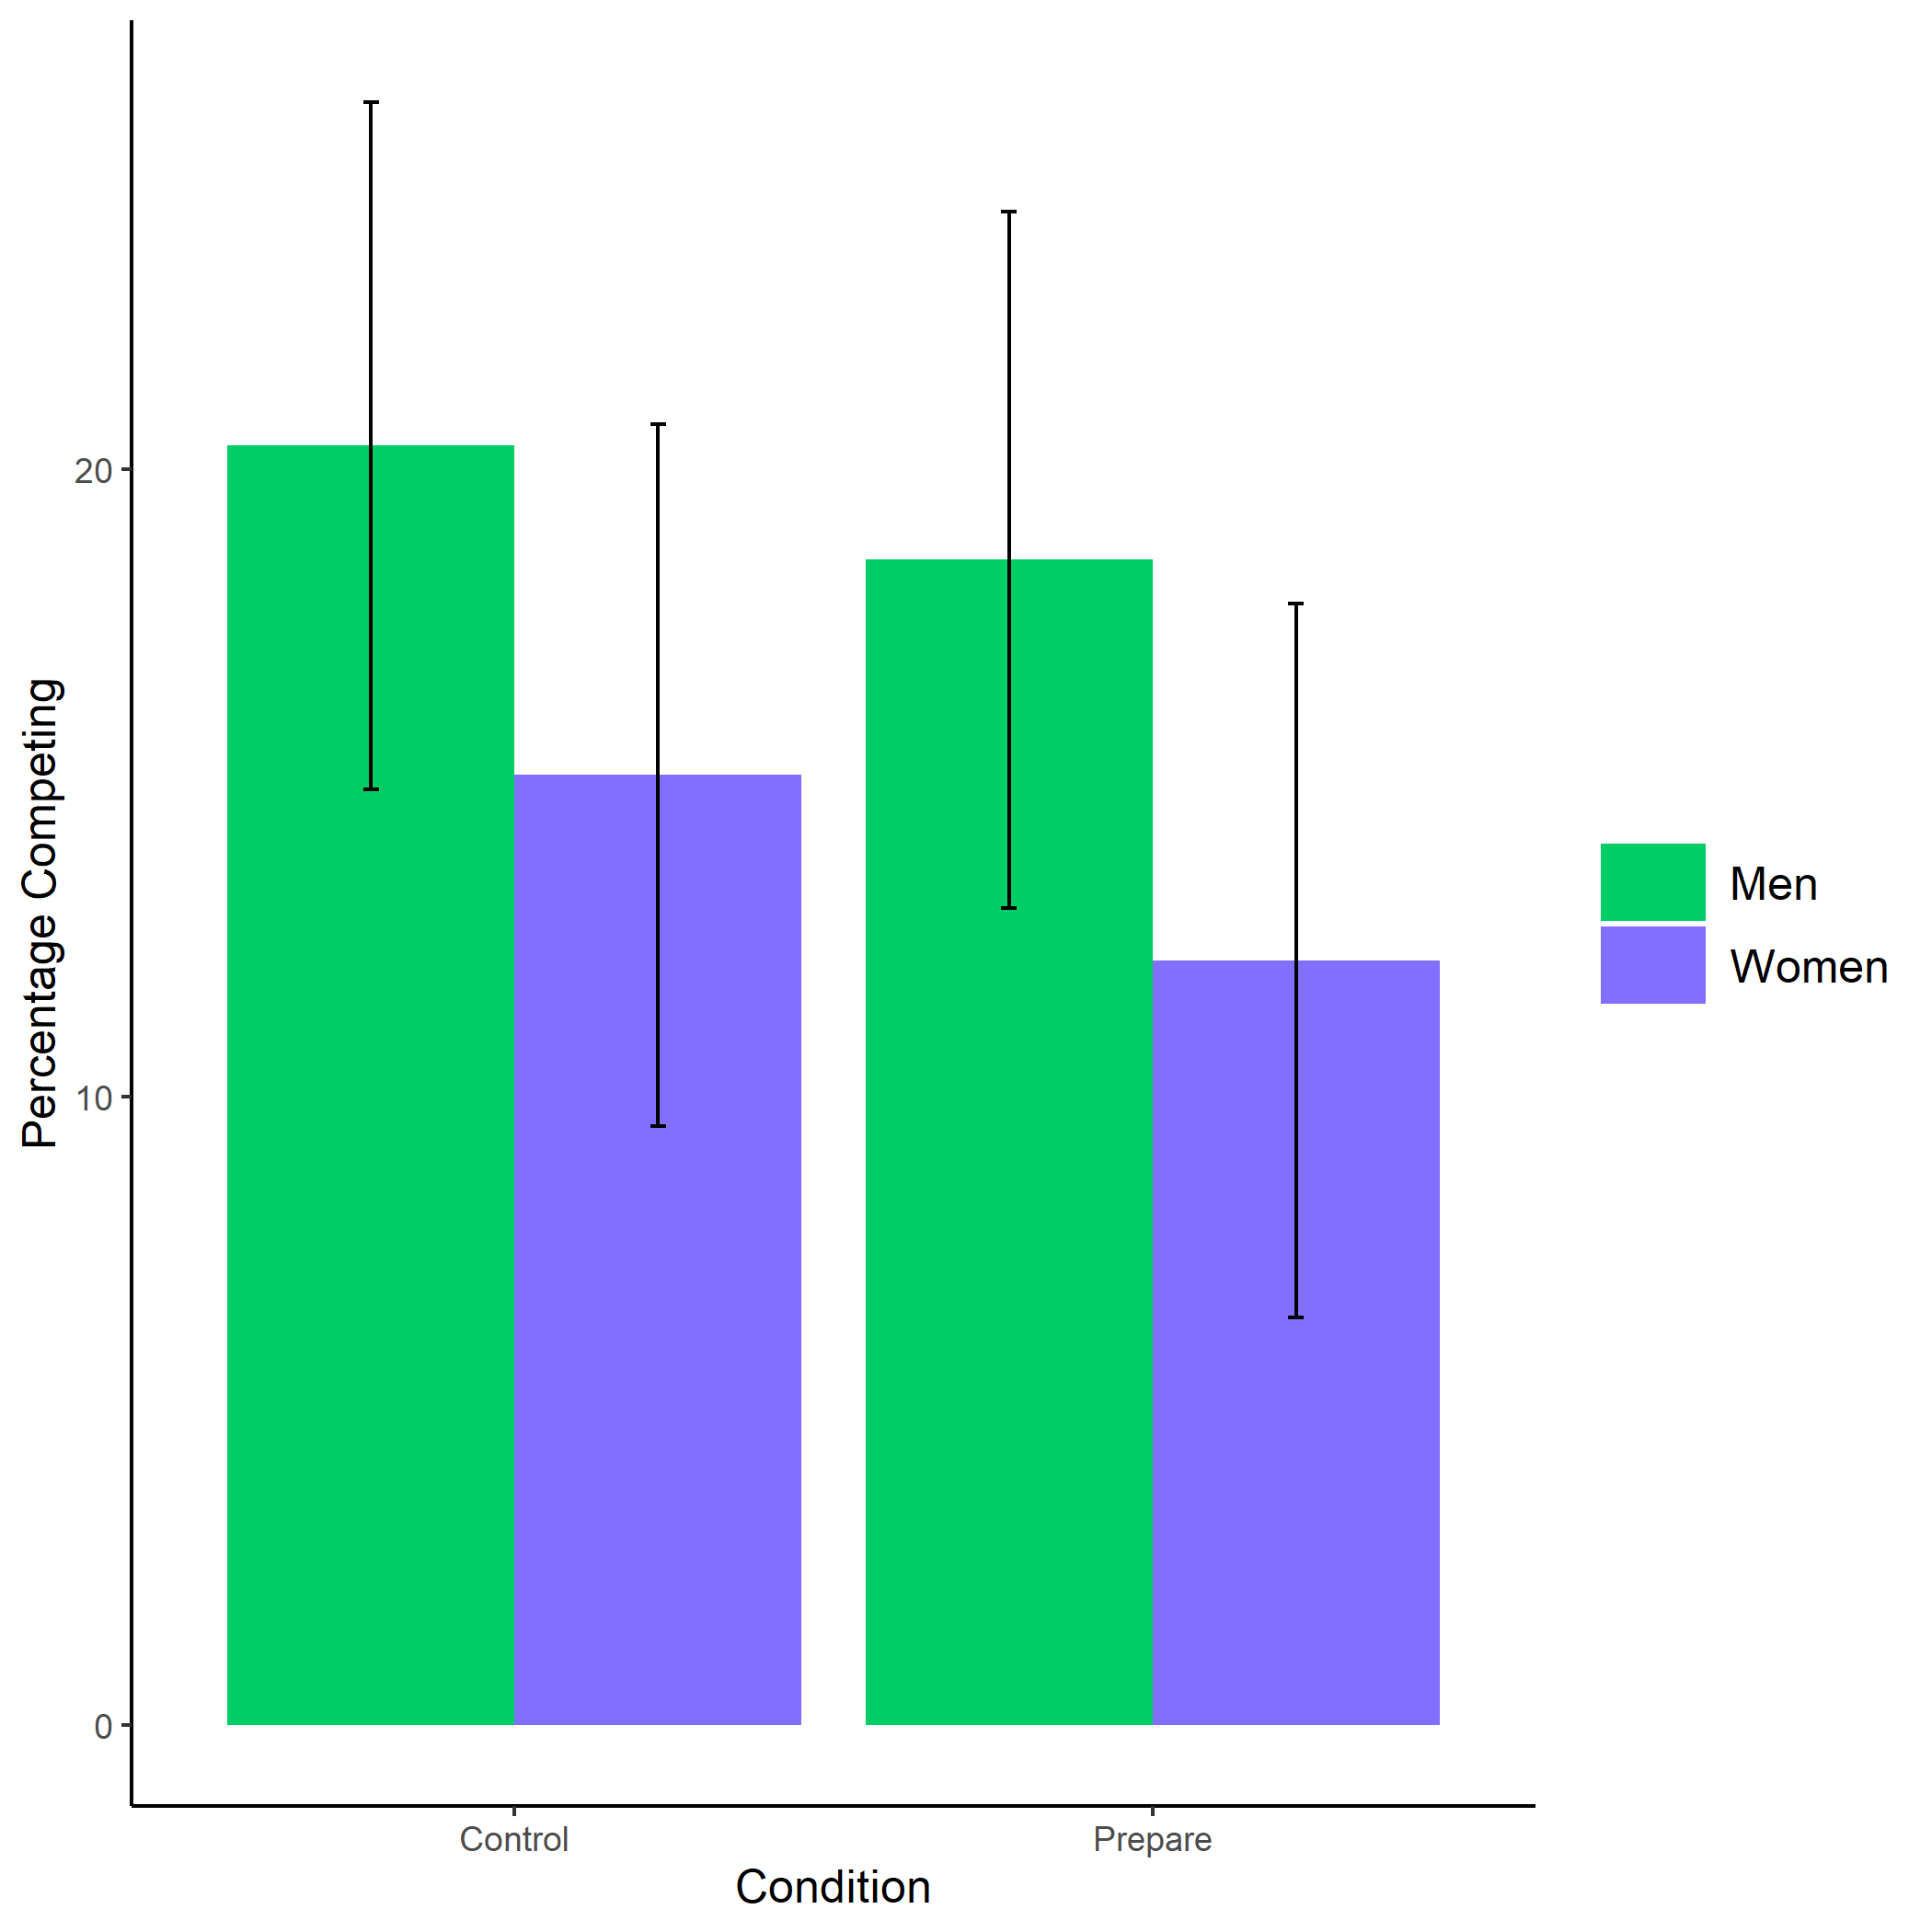
\includegraphics[width=300px]{C:/Users/keana/OneDrive - PennO365/Comp_transfer2018/Penn/practice_study/gender-practice/study2/figs/fig06_comp-choice-by-gender-and-cond-bar} 

}

\caption{Proportion of men and women in Study 2 who chose to compete based on preparation condition. Limited preparation did not reduce the gender difference in competitiveness. Error bars represent standard errors.}\label{fig:s200}
\end{figure}

\newpage

\hypertarget{gender-differences-in-preparation-2}{%
\subsubsection{Gender differences in preparation}\label{gender-differences-in-preparation-2}}

Despite no evidence for the effect of requiring people to prepare (i.e., condition) on the choice to compete across participants, we replicate the effect of gender on the choice to practice found in Study 1, where women were significantly more likely to opt-in to prepare for the task, even after being required to prepare in the preparation condition. 42.02\% of women across conditions chose to practice for the multiplication task beyond what was required, relative to 35.99\% of men, \(b = 0.25\), 95\% CI \([0.00\), \(0.50]\), \(z = 1.99\), \(p = .047\) (see right panel of Figure \ref{fig:panel-study2}). The gender effect holds even after controlling for the decision to compete and the interaction between gender and the decision to compete, \(b = 0.31\), 95\% CI \([0.03\), \(0.59]\), \(z = 2.17\), \(p = .030\) (see left panel of Figure \ref{fig:panel-study2}). Within the same model, we find that the choice to compete itself increases the likelihood a participant will practice before completing the paid task, \(b = 0.83\), 95\% CI \([0.39\), \(1.27]\), \(z = 3.70\), \(p < .001\), but no evidence of an interaction between gender and payment scheme choice, \(b = 0.04\), 95\% CI \([-0.63\), \(0.72]\), \(z = 0.12\), \(p = .906\). To see if the gender effect is explained by other variables included in the study, we added confidence, risk attitudes, and task scores to the previous model, and find that gender still significantly predicts the choice to practice, \(b = 0.41\), 95\% CI \([0.12\), \(0.71]\), \(z = 2.76\), \(p = .006\), over any effects of differences in risk attitudes, confidence, or task scores (see Table \ref{tab:tab-pract-choice-study2}). We ran the same two-part hurdle model described in Study 1 with gender, competition choice, and the interaction between those variables predicting the number of practice rounds variable. Again, we do not find evidence of gender differences in the choice to continue preparing after the initial decision to prepare, \emph{b} = -0.14, 95\% CI {[}-0.53, 0.25{]}, \emph{z} = -0.71, \emph{p} = 0.48.

\begin{figure}

{\centering 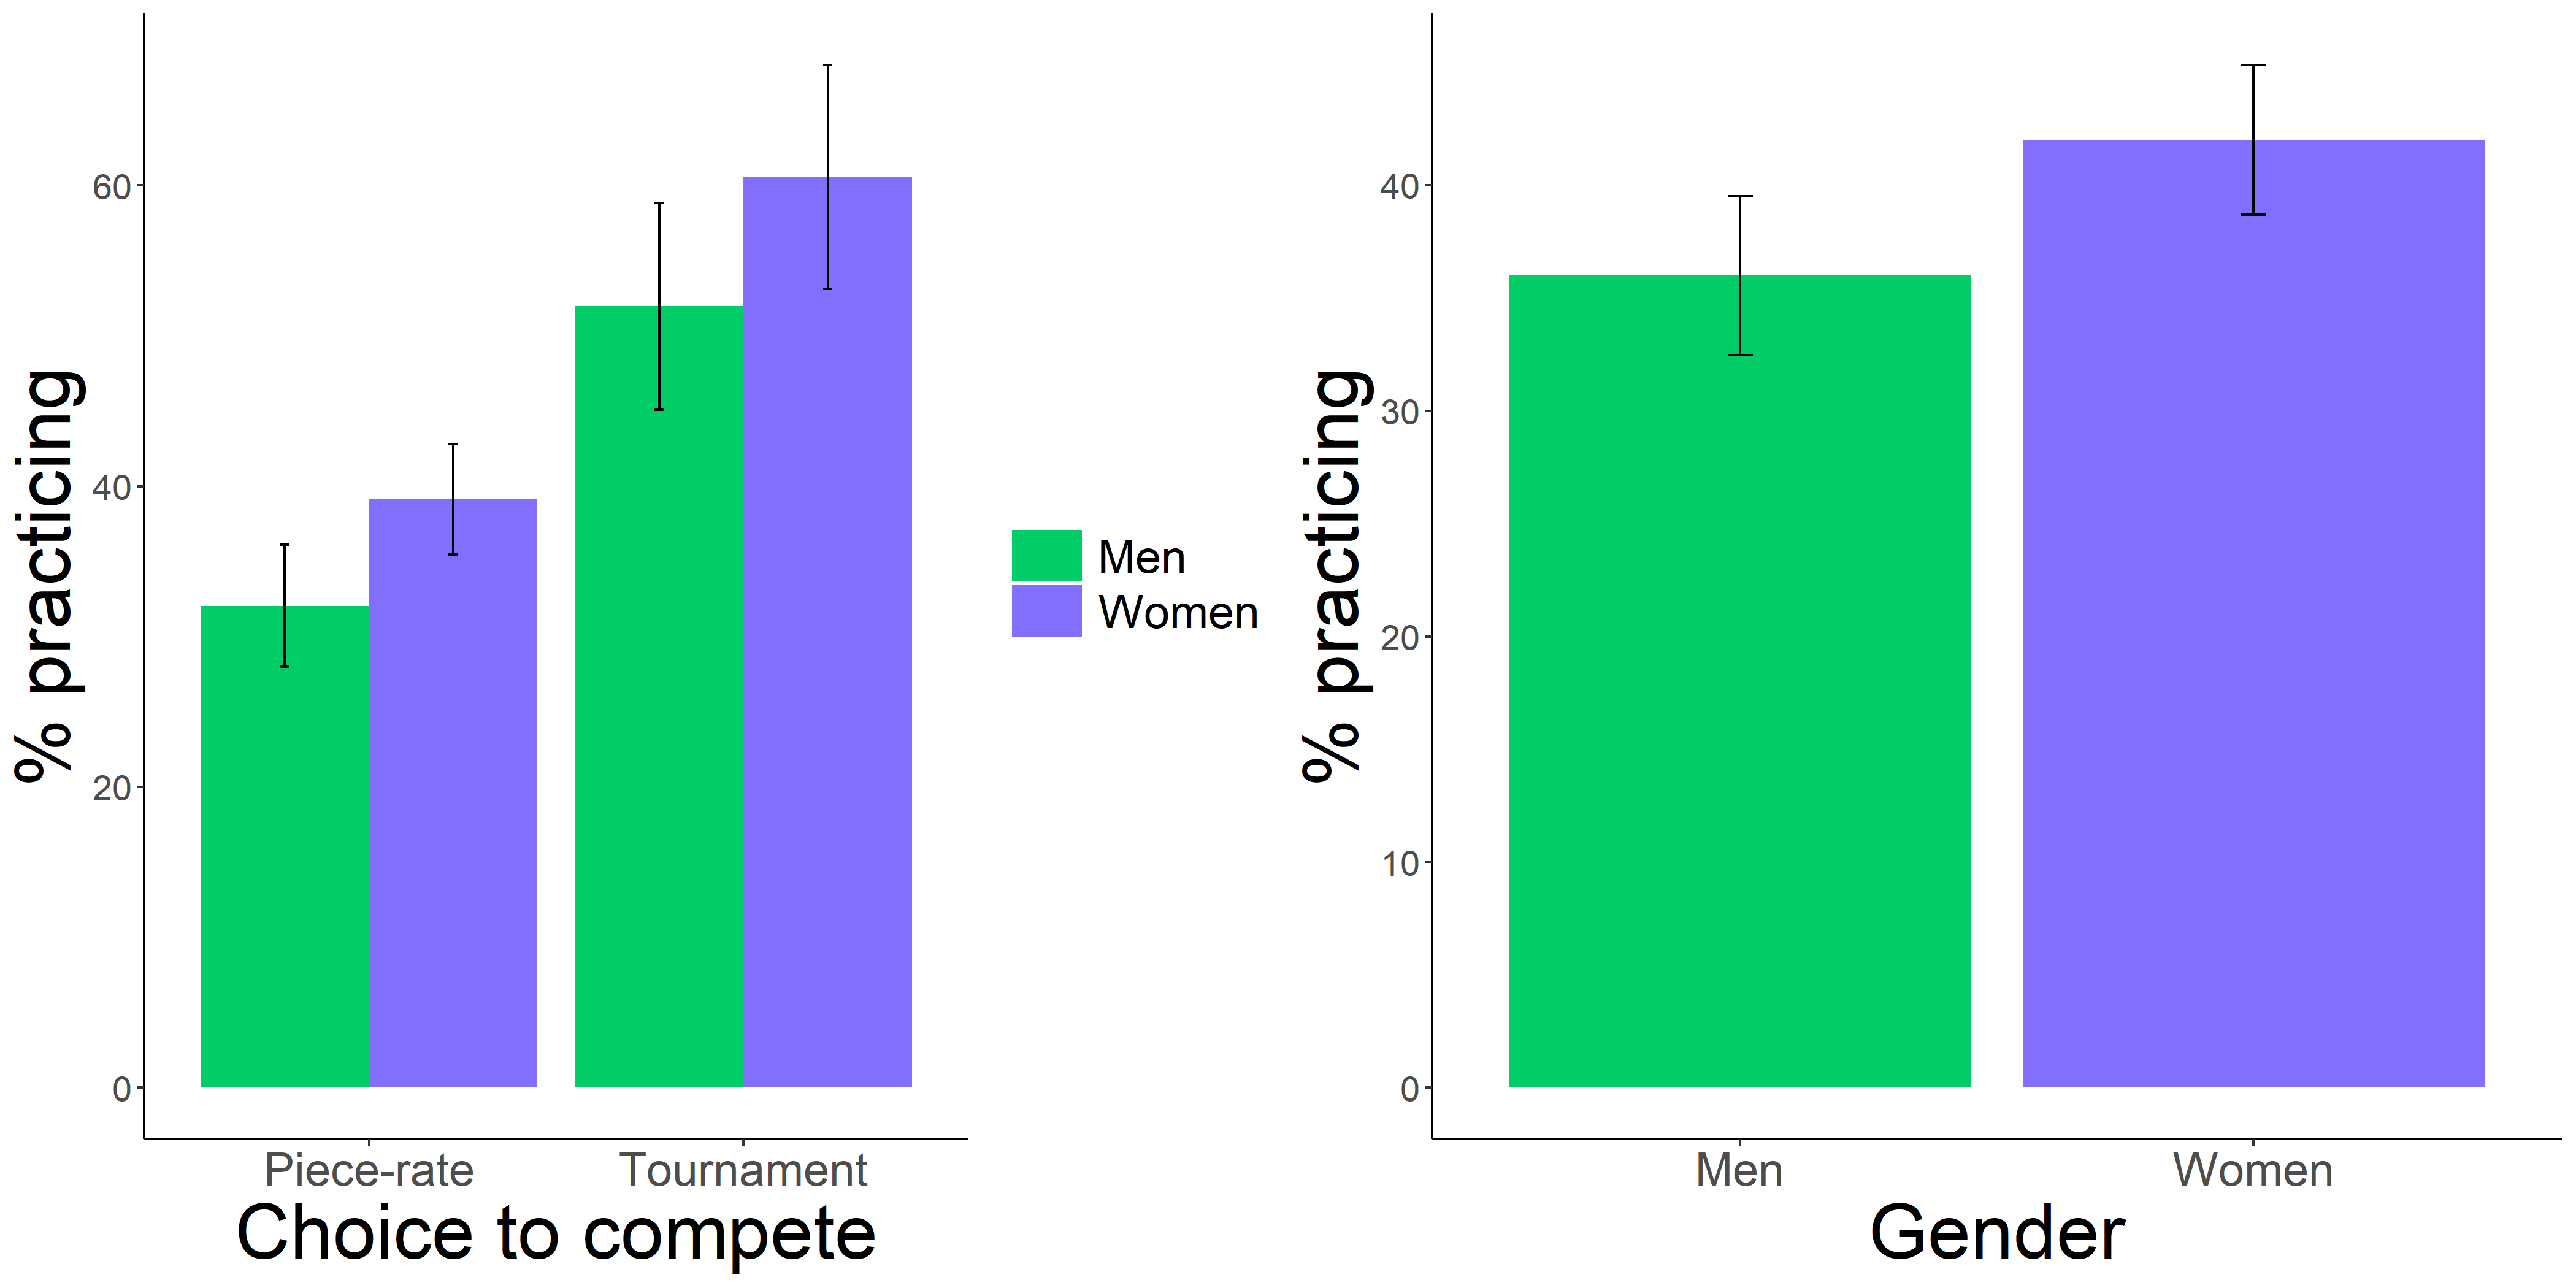
\includegraphics[width=1\linewidth]{C:/Users/keana/OneDrive - PennO365/Comp_transfer2018/Penn/practice_study/gender-practice/study2/figs/panel_study2} 

}

\caption{Right panel shows the proportion of men and women in Study 2 who chose to prepare. Left panel shows the proportion of men and women in Study 2 who chose to prepare based on choice to compete. Women choose to prepare more than men, regardless of their decision to compete. Error bars represent standard errors.}\label{fig:panel-study2}
\end{figure}
\newpage

\begin{center}
\includegraphics[width=1\linewidth]{C:/Users/keana/OneDrive - PennO365/Comp_transfer2018/Penn/practice_study/gender-practice/study2/figs/tab_pract-choice-study2} \end{center}

\begin{table}[ht]
\centering
\begingroup\fontsize{0.1pt}{0.1pt}\selectfont
\begin{tabular}{r}
   \\ 
 \end{tabular}
\endgroup
\caption{All models are logistic regressions with choice to prepare as the dependent variable, where man and piece-rate payment scheme are the reference categories for participant gender and competition choice, respectively. Women prepare more than men regardless of competition choice, task score, risk attitudes, or confidence. p < .05 is considered significant and bolded.} 
\label{tab:tab-pract-choice-study2}
\end{table}

\hypertarget{perceptions-of-gender-differences-in-preparation-performance-and-competitiveness-2}{%
\subsubsection{Perceptions of gender differences in preparation, performance, and competitiveness}\label{perceptions-of-gender-differences-in-preparation-performance-and-competitiveness-2}}

Again, we find that these results align with participants' expectations, where they were significantly more likely to expect women (with 85.38\% selecting women versus 14.62\% selecting men) to choose to prepare more than men both in general, \(\chi^2(1, n = 1088) = 513.72\), \(p < .001\) (see Figure \ref{fig:s206}), and on the paid multiplication task, \(\chi^2(1, n = 1088) = 394.33\), \(p < .001\) (see Figure \ref{fig:s203}) (with 80.95\% selecting women versus 19.05\% selecting men), despite expecting men to choose to compete more often, \(\chi^2(1, n = 1088) = 580.69\), \(p < .001\) (see Figure \ref{fig:s205}) and expecting no gender differences in performance on the task, \(\chi^2(1, n = 1088) = 0.51\), \(p = .473\) (see Figure \ref{fig:s204}). See Table \ref{tab:summary-table-beliefs-study2} for a summary of participants' responses to the questions about gender differences in preparation, performance, and competitiveness.

\begin{center}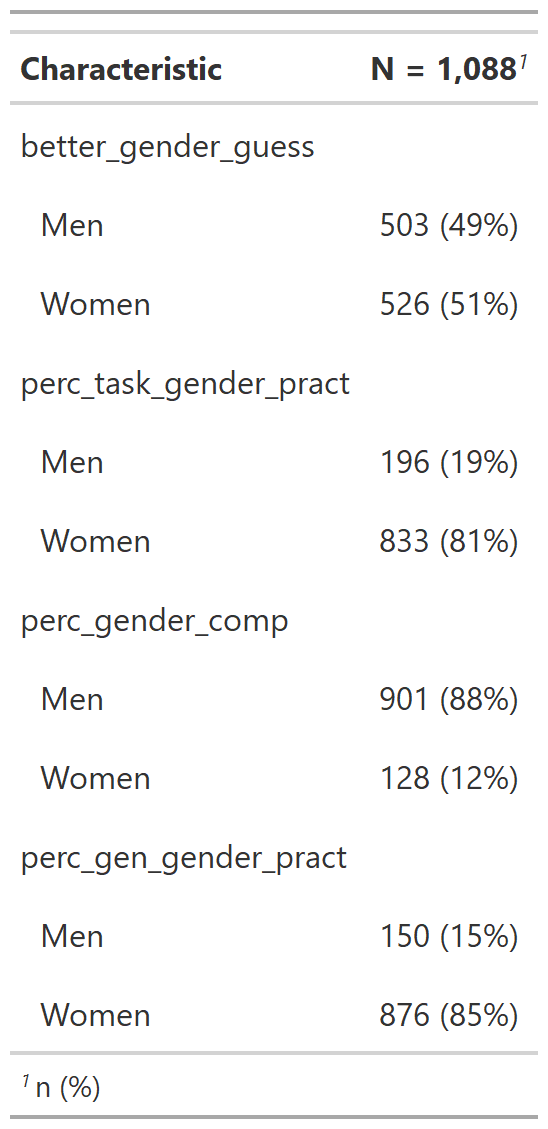
\includegraphics[width=0.35\linewidth]{C:/Users/keana/OneDrive - PennO365/Comp_transfer2018/Penn/practice_study/gender-practice/study2/figs/summary-table-beliefs-study2} \end{center}

\begin{table}[ht]
\centering
\begingroup\fontsize{0.1pt}{0.1pt}\selectfont
\begin{tabular}{r}
   \\ 
 \end{tabular}
\endgroup
\caption{Number and percentage of participants that selected each respective option when asked which gender would correctly solve more problems on the multiplication task, spend more time preparing for the multiplication task, choose the tournament payment scheme more often, and spend more time preparing on most tasks.} 
\label{tab:summary-table-beliefs-study2}
\end{table}

\begin{figure}

{\centering 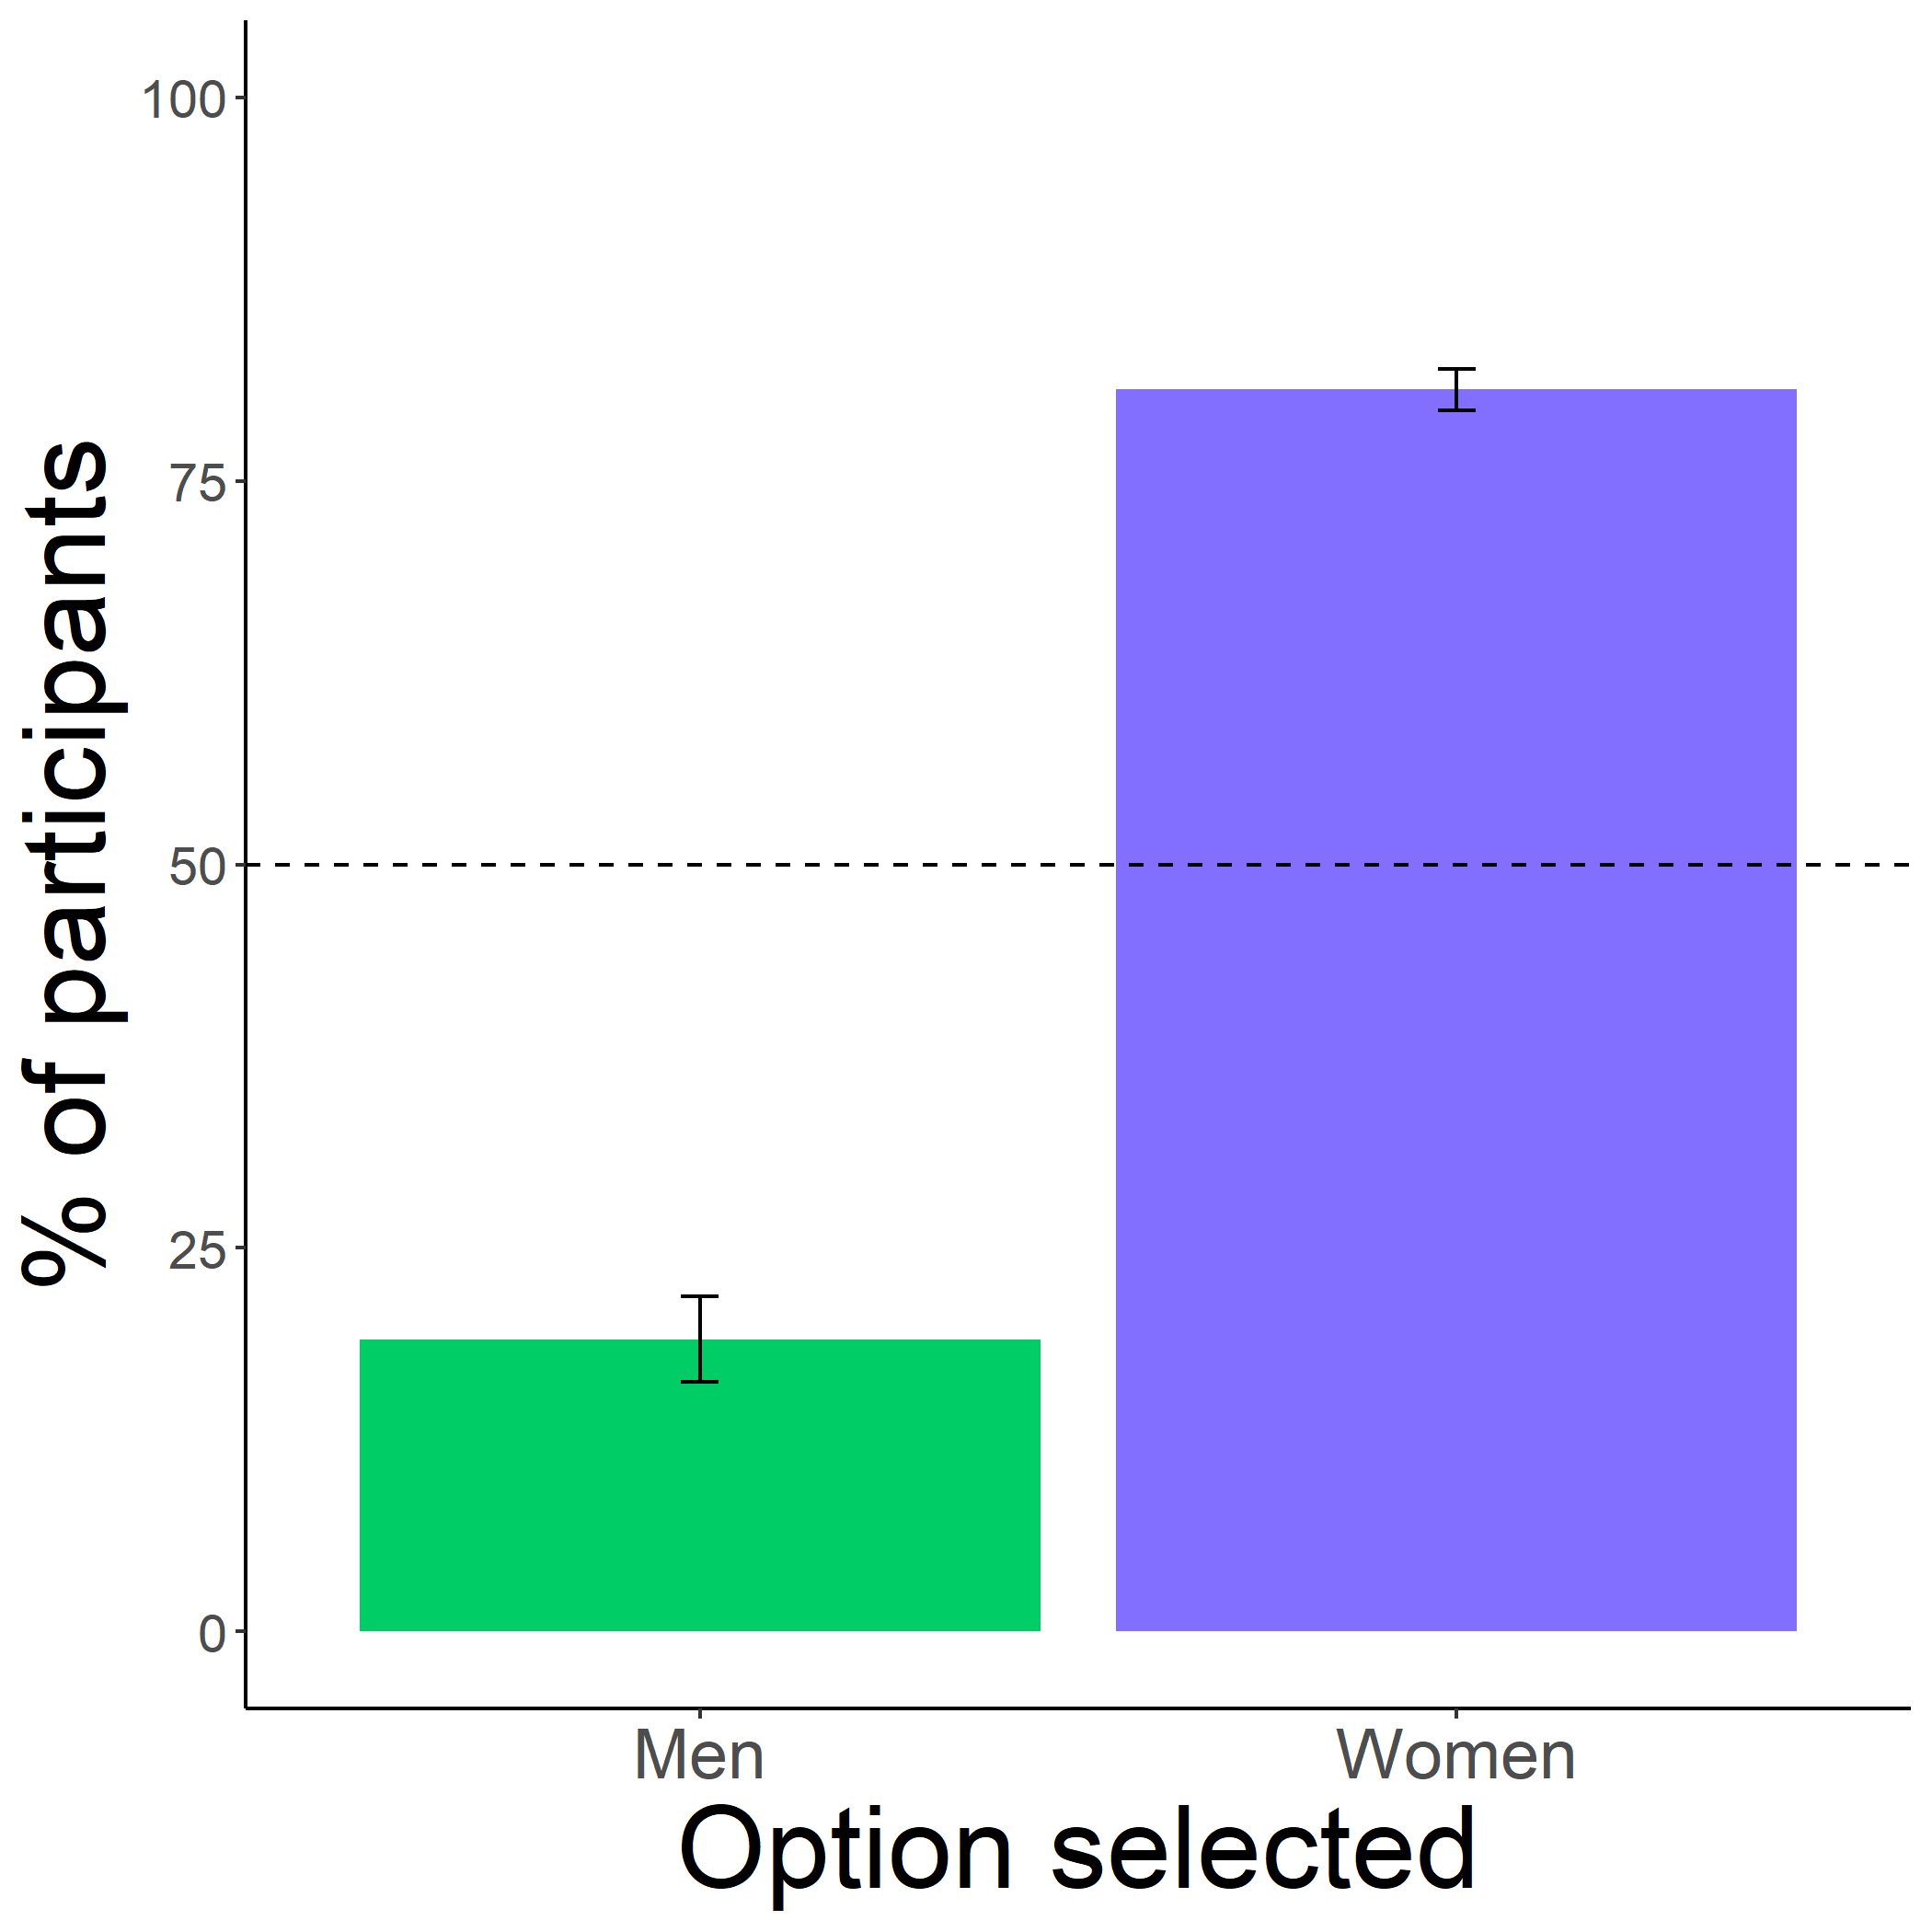
\includegraphics[width=300px]{C:/Users/keana/OneDrive - PennO365/Comp_transfer2018/Penn/practice_study/gender-practice/study2/figs/fig08_perc-task-gender-pract} 

}

\caption{Proportion of participants that predicted women or men would spend more time preparing for the multiplication task. A significantly larger proportion of participants expected women to spend more time preparing for the multiplication task. Error bars represent standard errors.}\label{fig:s203}
\end{figure}

\begin{figure}

{\centering 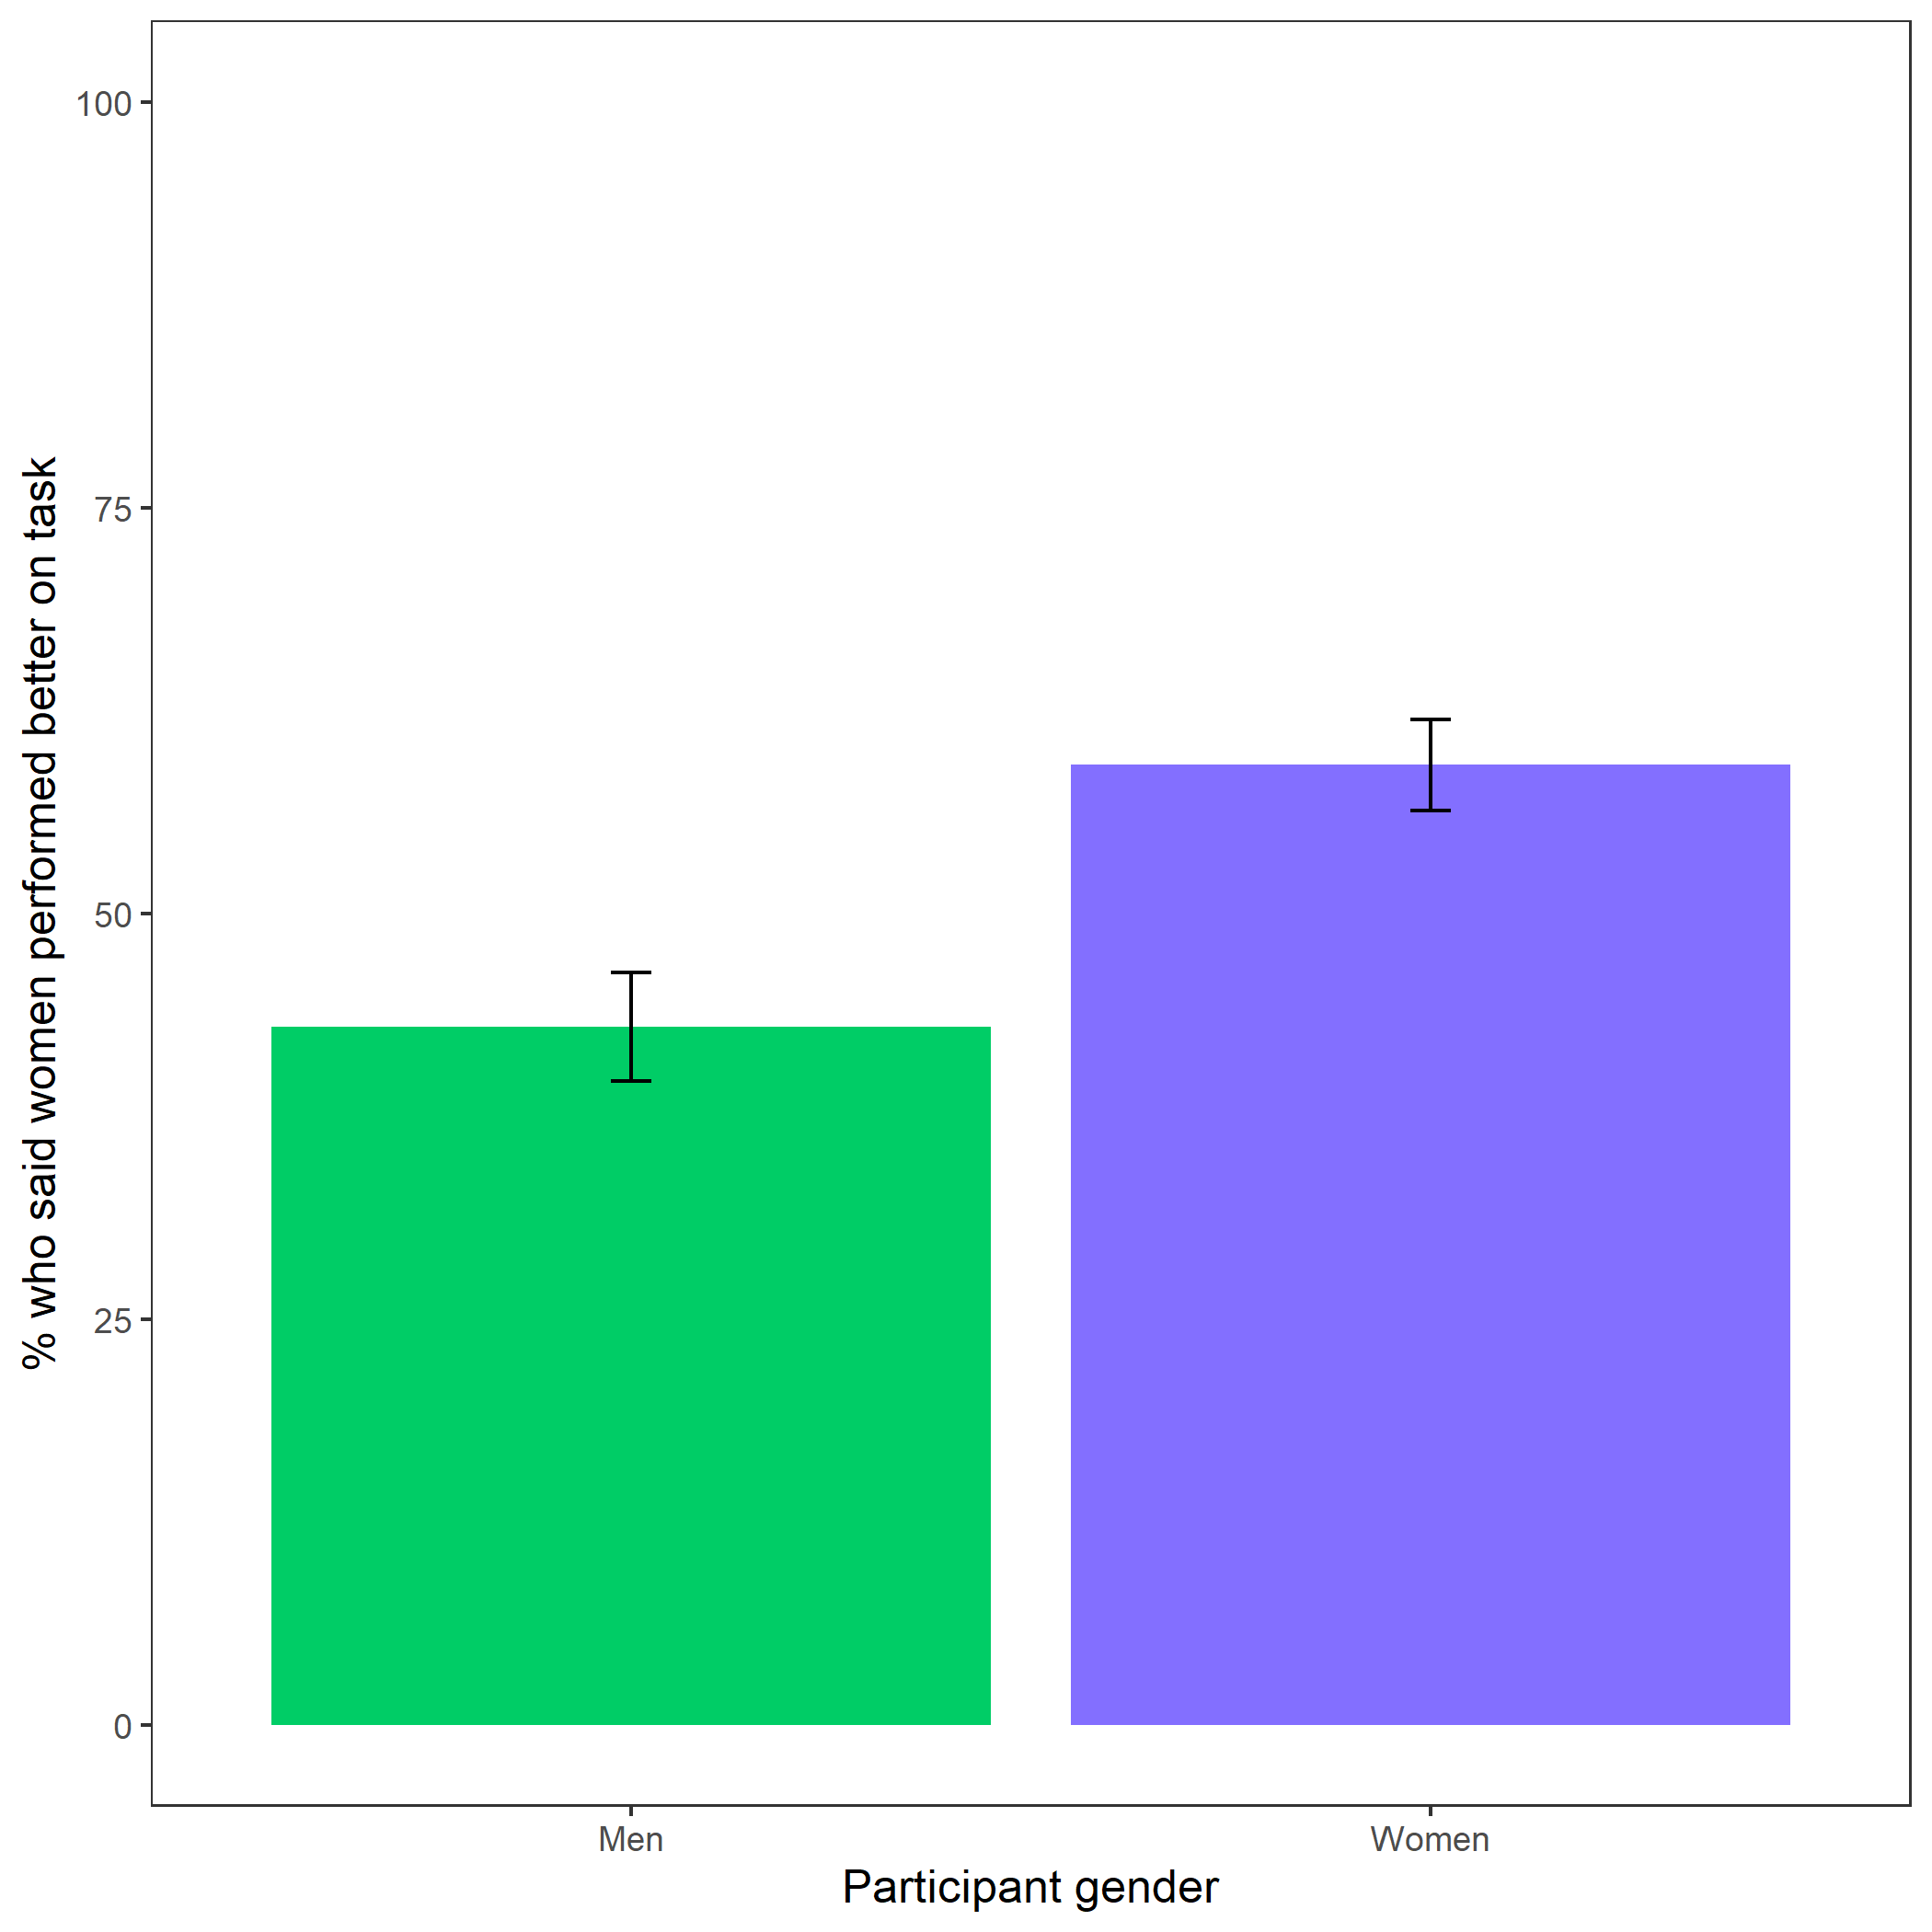
\includegraphics[width=300px]{C:/Users/keana/OneDrive - PennO365/Comp_transfer2018/Penn/practice_study/gender-practice/study2/figs/fig01_better-gender-guess} 

}

\caption{Proportion of participants that predicted women or men would correctly solve more problems on the multiplication task. There was no significant difference in the proportion of participants that expected women or men to perform better on the multiplication task. Error bars represent standard errors.}\label{fig:s204}
\end{figure}

\begin{figure}

{\centering 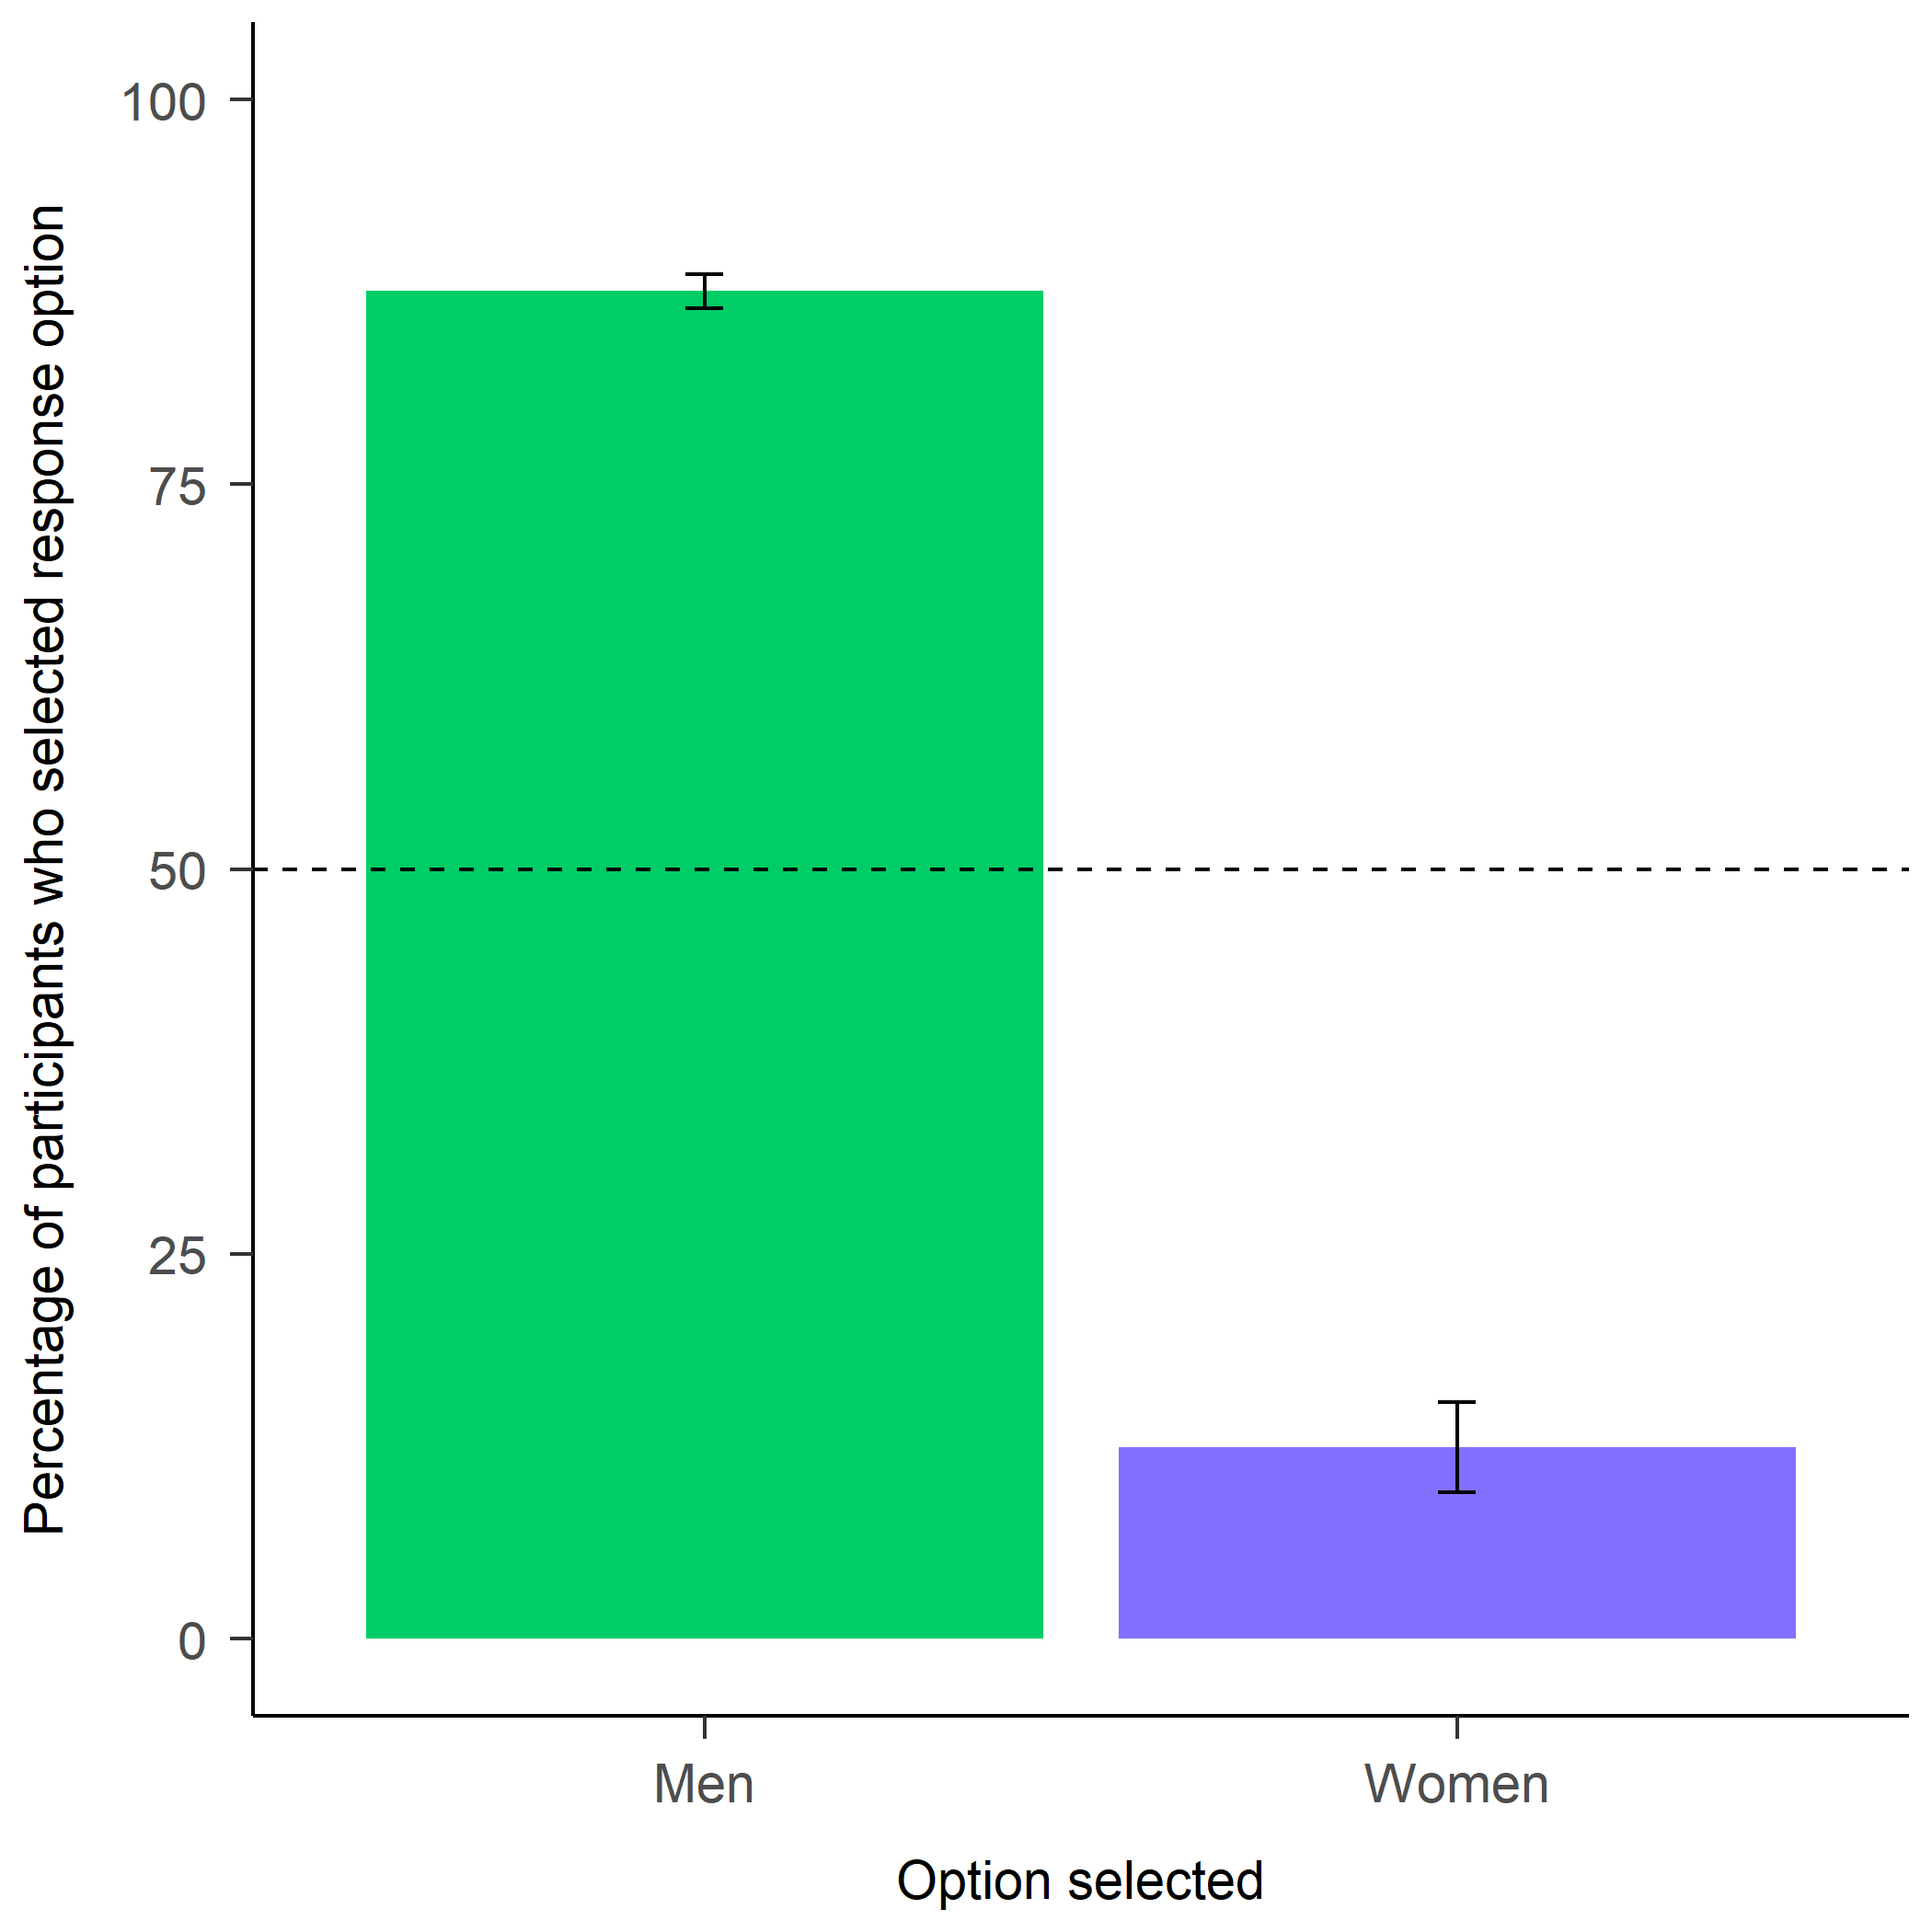
\includegraphics[width=300px]{C:/Users/keana/OneDrive - PennO365/Comp_transfer2018/Penn/practice_study/gender-practice/study2/figs/fig02_perc-gender-comp} 

}

\caption{Proportion of participants that predicted women or men would choose to compete. A significantly larger proportion of participants expected men to be more likely to choose to compete. Error bars represent standard errors.}\label{fig:s205}
\end{figure}

\begin{figure}

{\centering 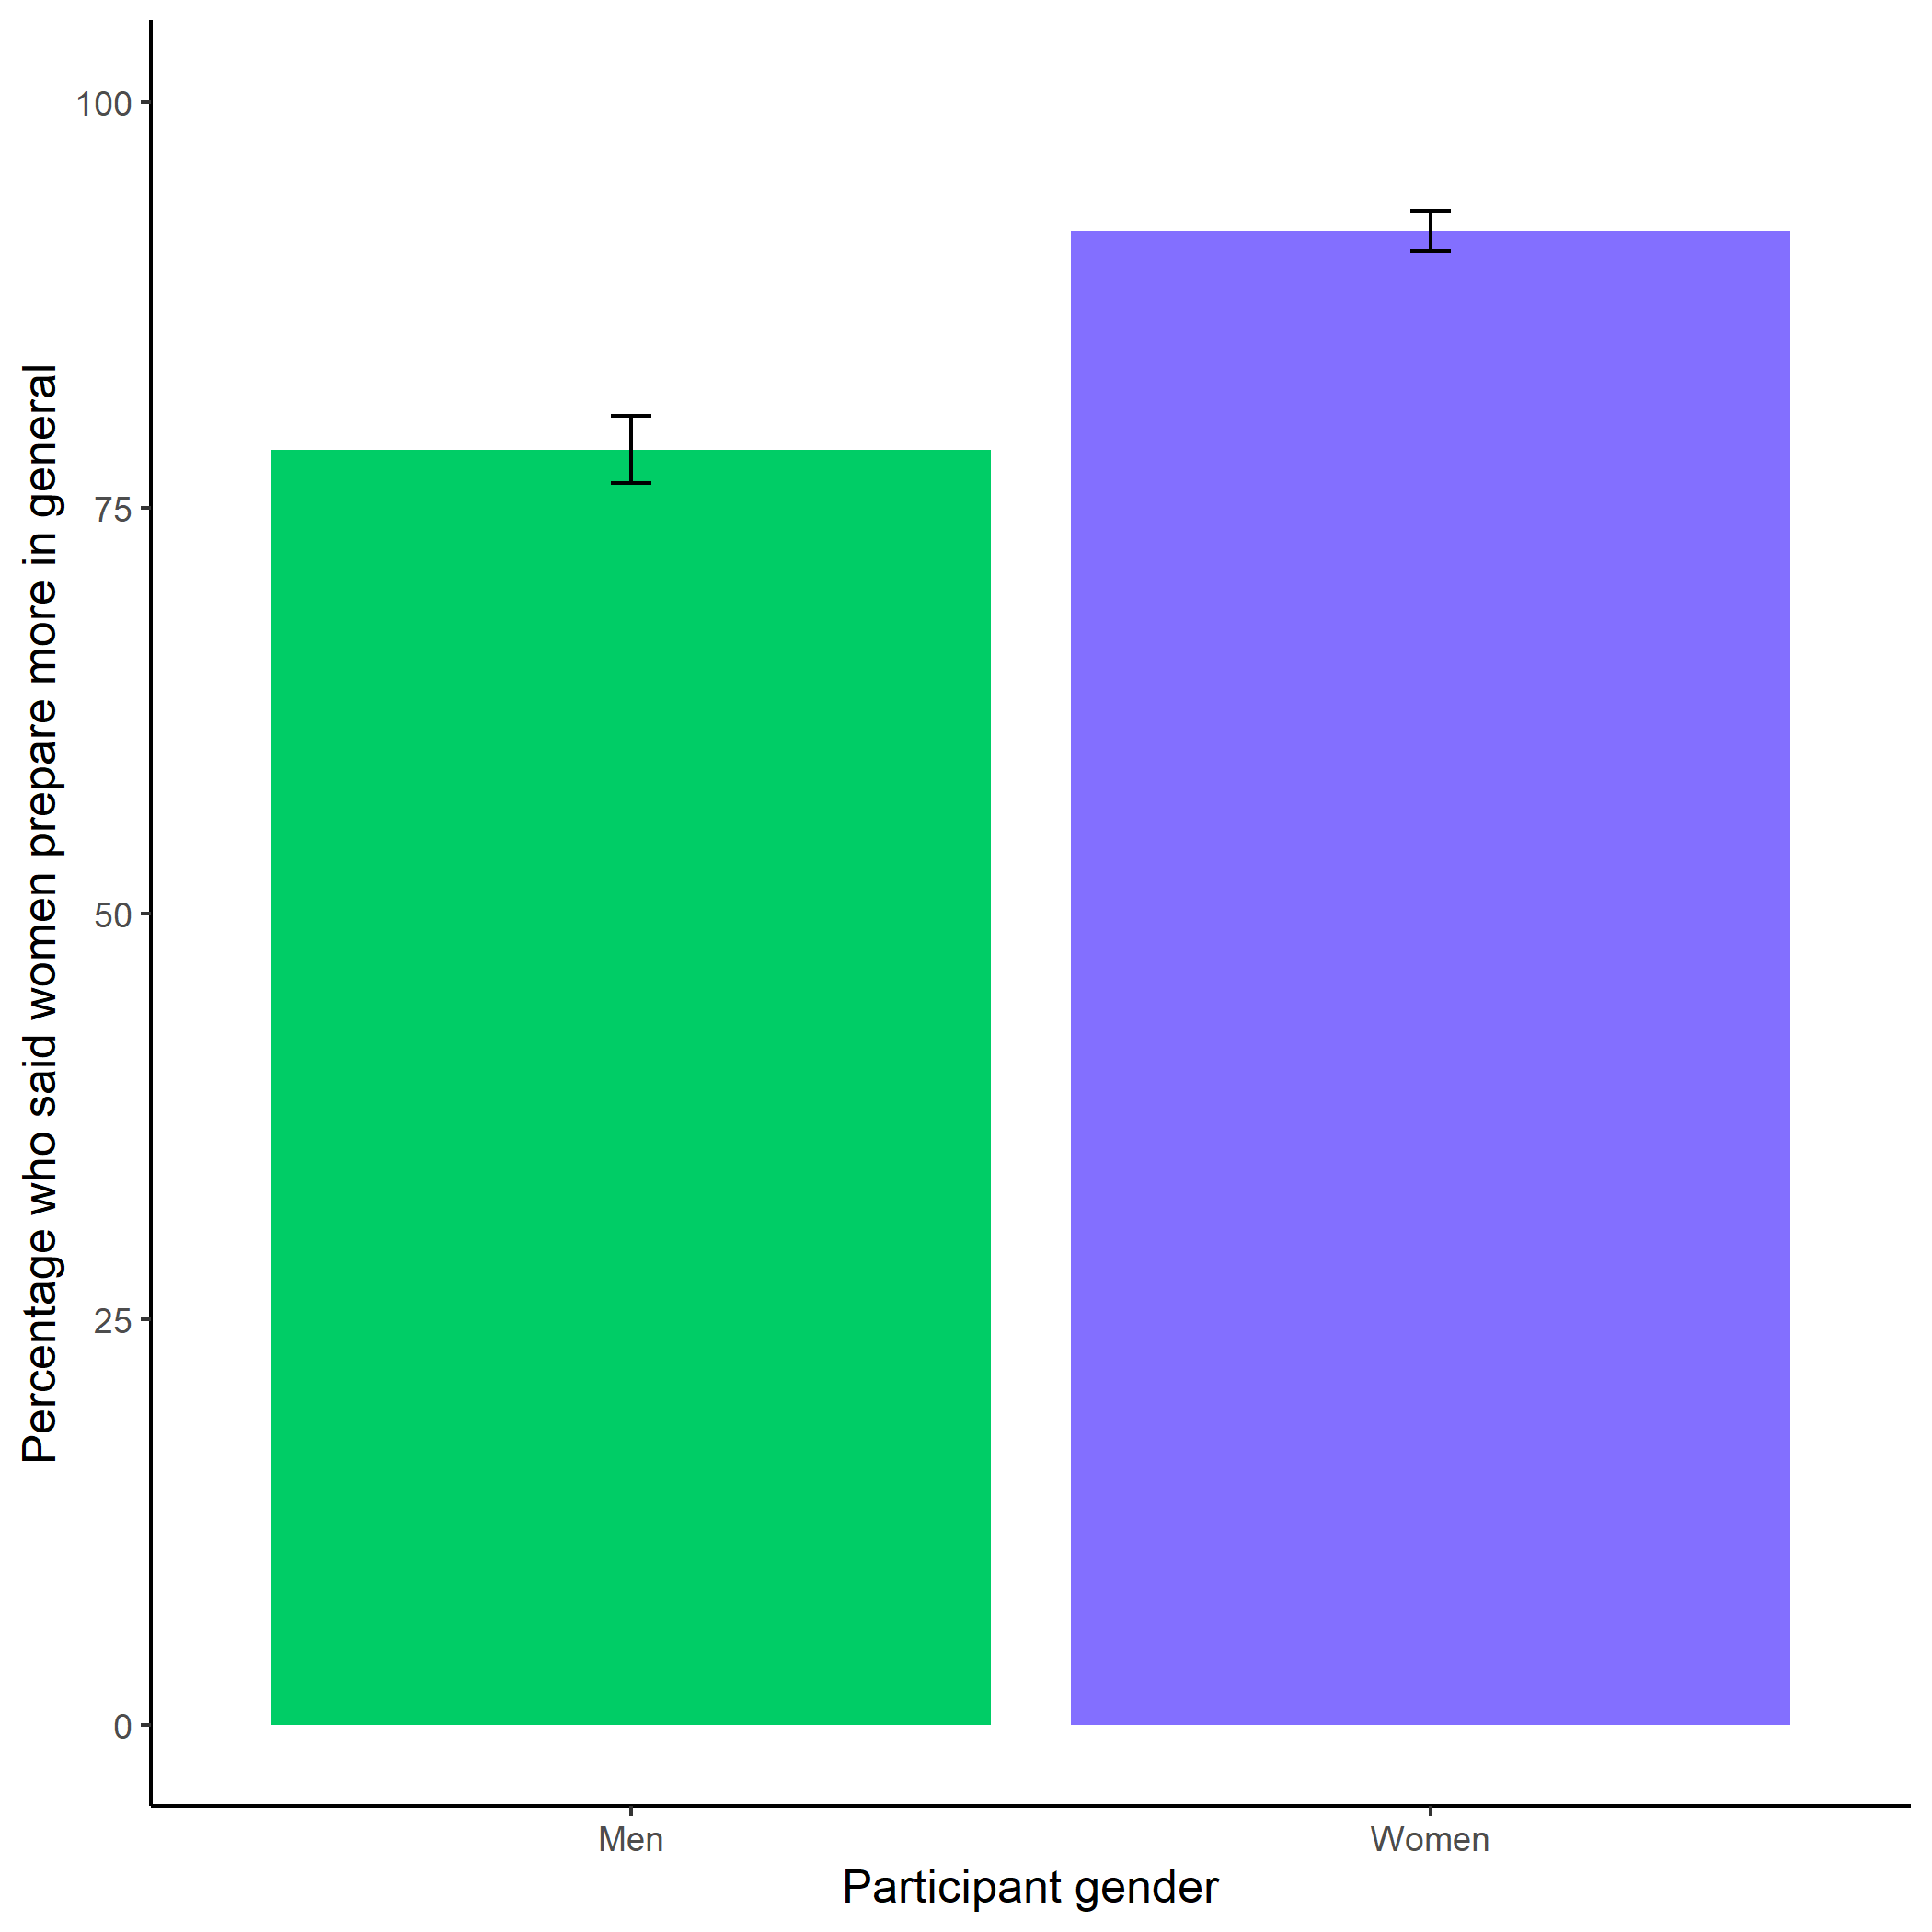
\includegraphics[width=300px]{C:/Users/keana/OneDrive - PennO365/Comp_transfer2018/Penn/practice_study/gender-practice/study2/figs/fig03_perc-gen-gender-pract} 

}

\caption{Proportion of participants that predicted women or men would spend more time preparing on most tasks. A significantly larger proportion of participants expected women to spend more time preparing on most tasks. Error bars represent standard errors.}\label{fig:s206}
\end{figure}

\hypertarget{effects-of-gender-and-perceptions-on-practicing-2}{%
\subsubsection{Effects of gender and perceptions on practicing}\label{effects-of-gender-and-perceptions-on-practicing-2}}

Like Study 1, we explored whether women who believed other women prepare more were especially likely to prepare. To that end, we ran a logistic regression with the choice to practice as the dependent variable and gender, beliefs about gender differences in preparation on most tasks, and the interaction between those two variables as the predictors. We replicate the interaction effect found in Study 1, such that women who said women generally prepare more on most tasks were especially likely to prepare, \(b = 1.21\), 95\% CI \([0.42\), \(2.04]\), \(z = 2.94\), \(p = .003\) (see Figure \ref{fig:pract-choice-by-gender-and-perc-gen-prep-bar-study2}). We ran the same analysis with participants' beliefs about gender differences in preparation for the multiplication task, gender, and the interaction between the two as predictors instead, and replicate the interaction effect from the previous study, \(b = 1.52\), 95\% CI \([0.86\), \(2.18]\), \(z = 4.51\), \(p < .001\), such that women who said women spent more time preparing for the multiplication task were especially likely to prepare (see Figure \ref{fig:pract-choice-by-gender-and-perc-task-prep-bar-study2}).

\begin{figure}

{\centering 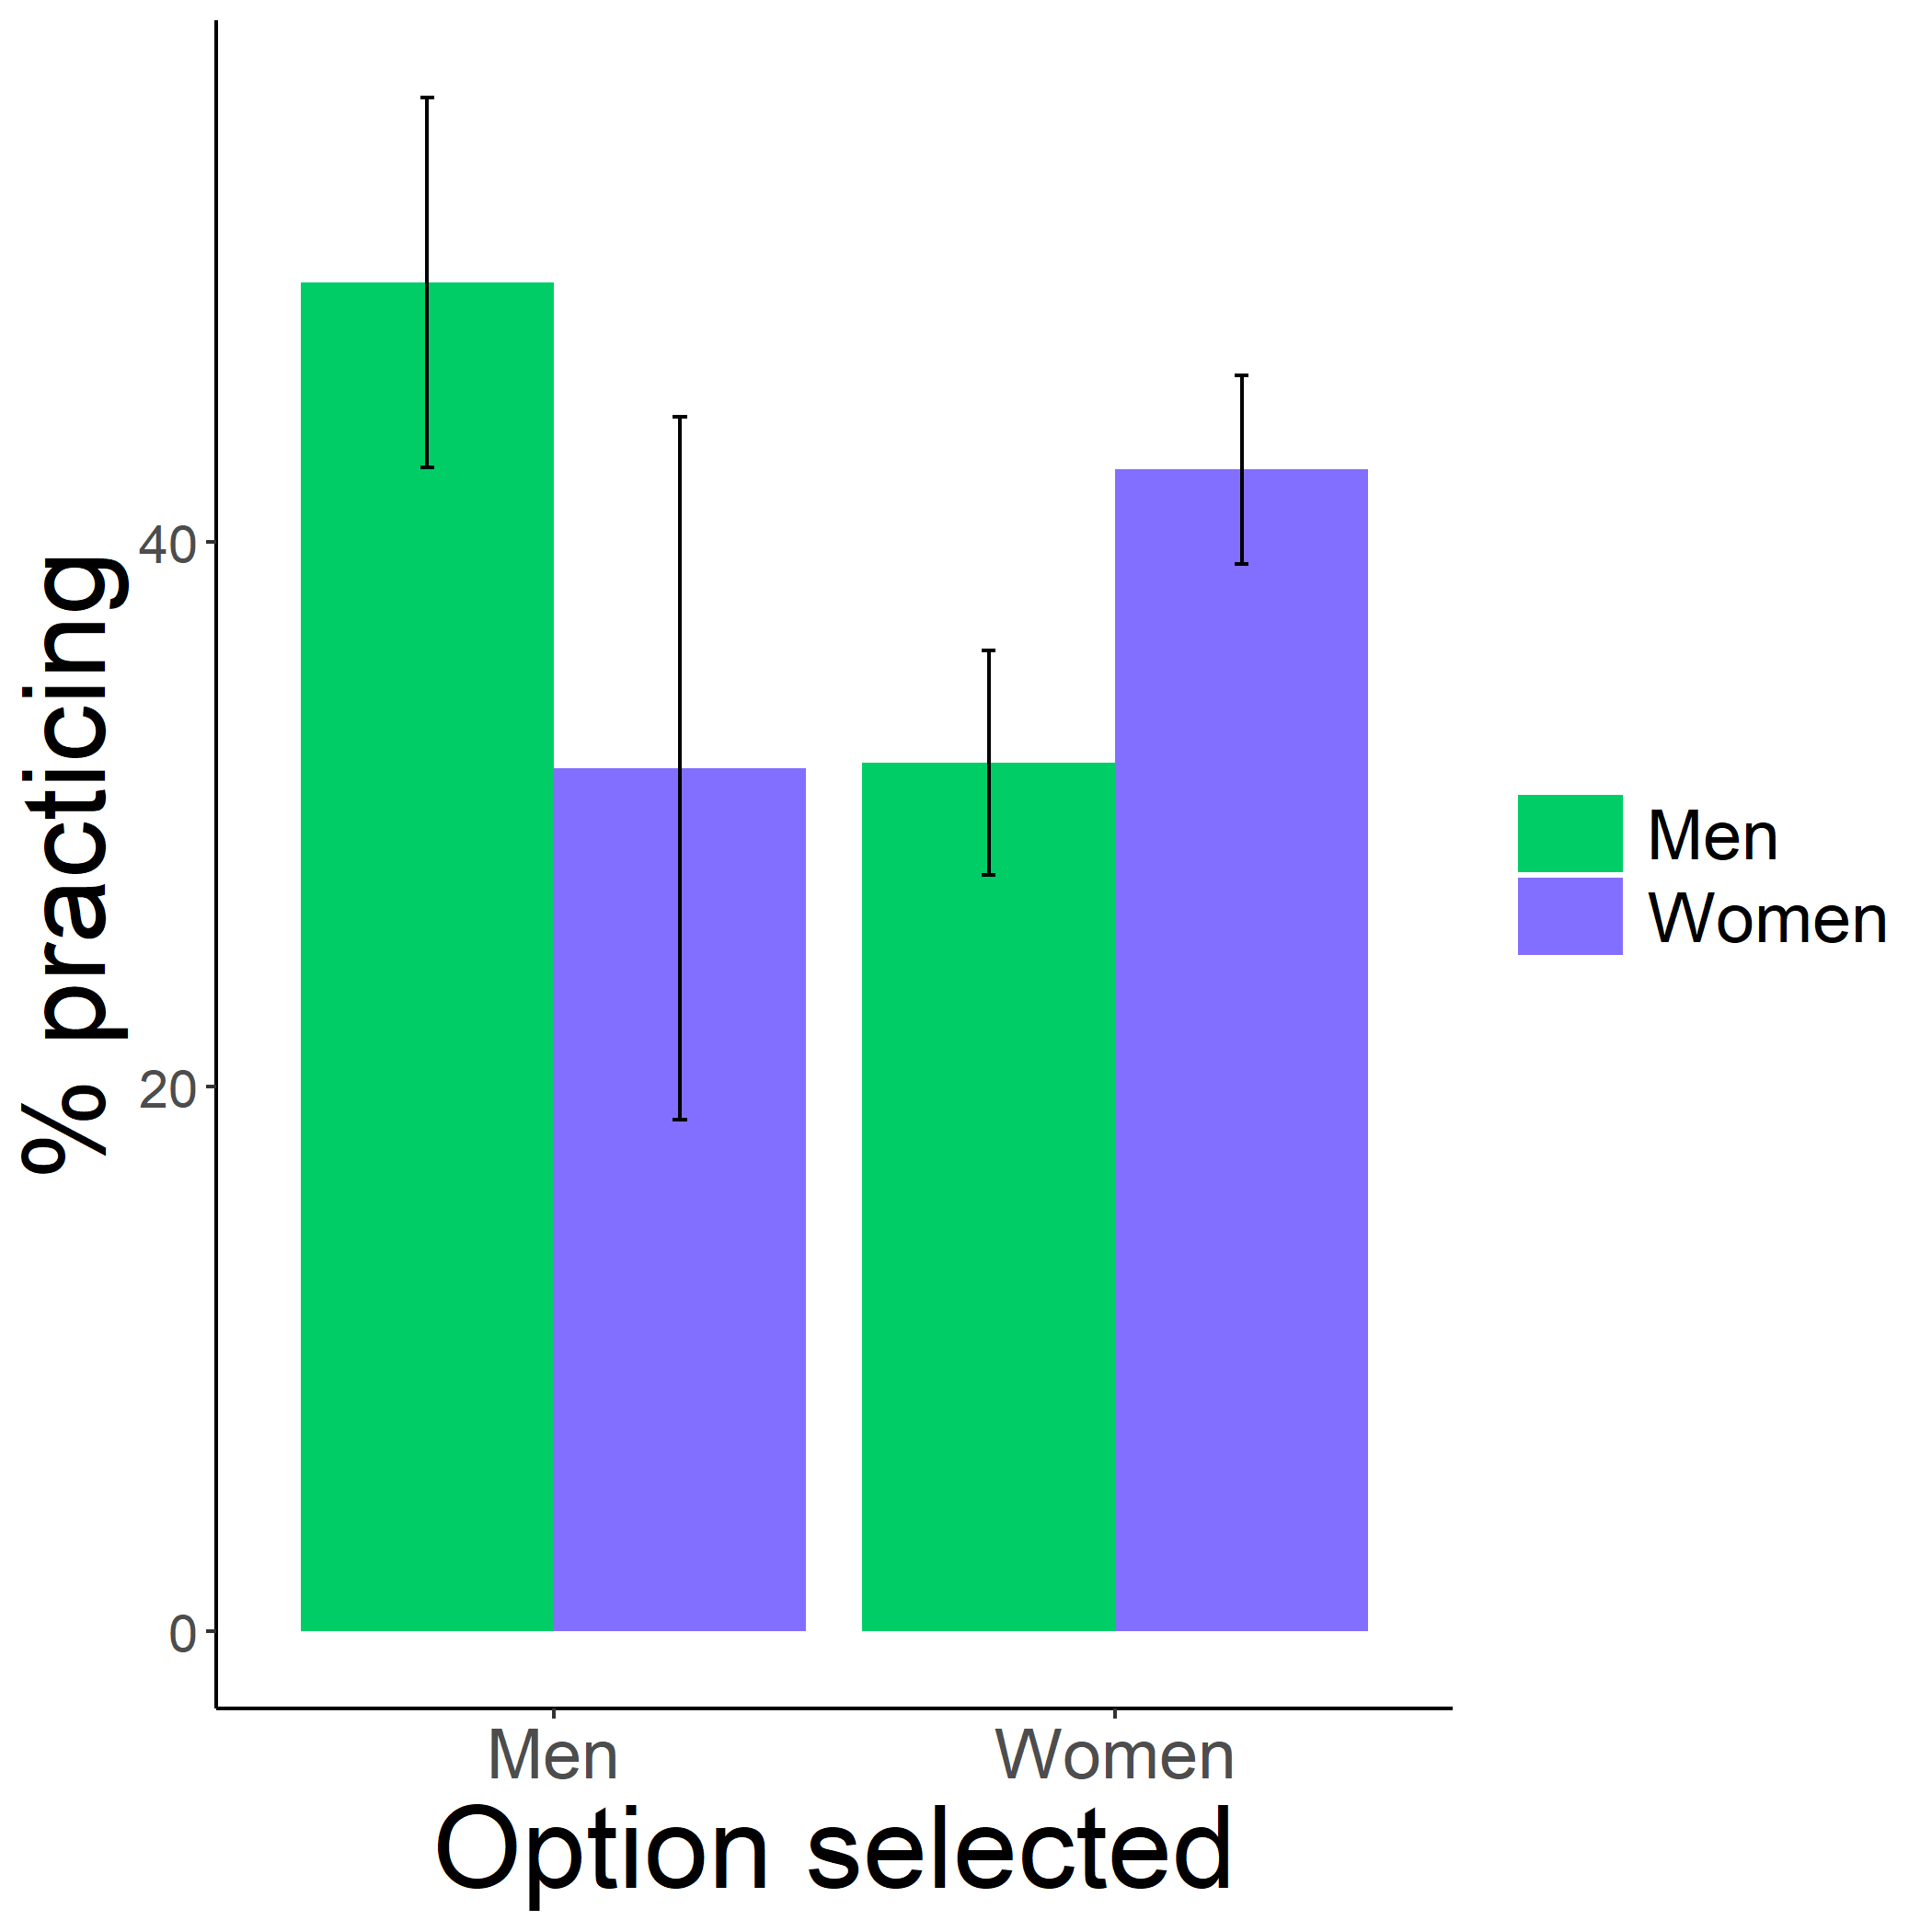
\includegraphics[width=300px]{C:/Users/keana/OneDrive - PennO365/Comp_transfer2018/Penn/practice_study/gender-practice/study2/figs/pract-choice-by-gender-and-perc-gen-prep-bar-study2} 

}

\caption{Proportion of men and women in Study 2 who chose to practice based on whether they thought men or women spend more time preparing on most tasks. Women who thought women generally prepare more were especially likely to choose to practice. Error bars represent standard errors.}\label{fig:pract-choice-by-gender-and-perc-gen-prep-bar-study2}
\end{figure}

\begin{figure}

{\centering 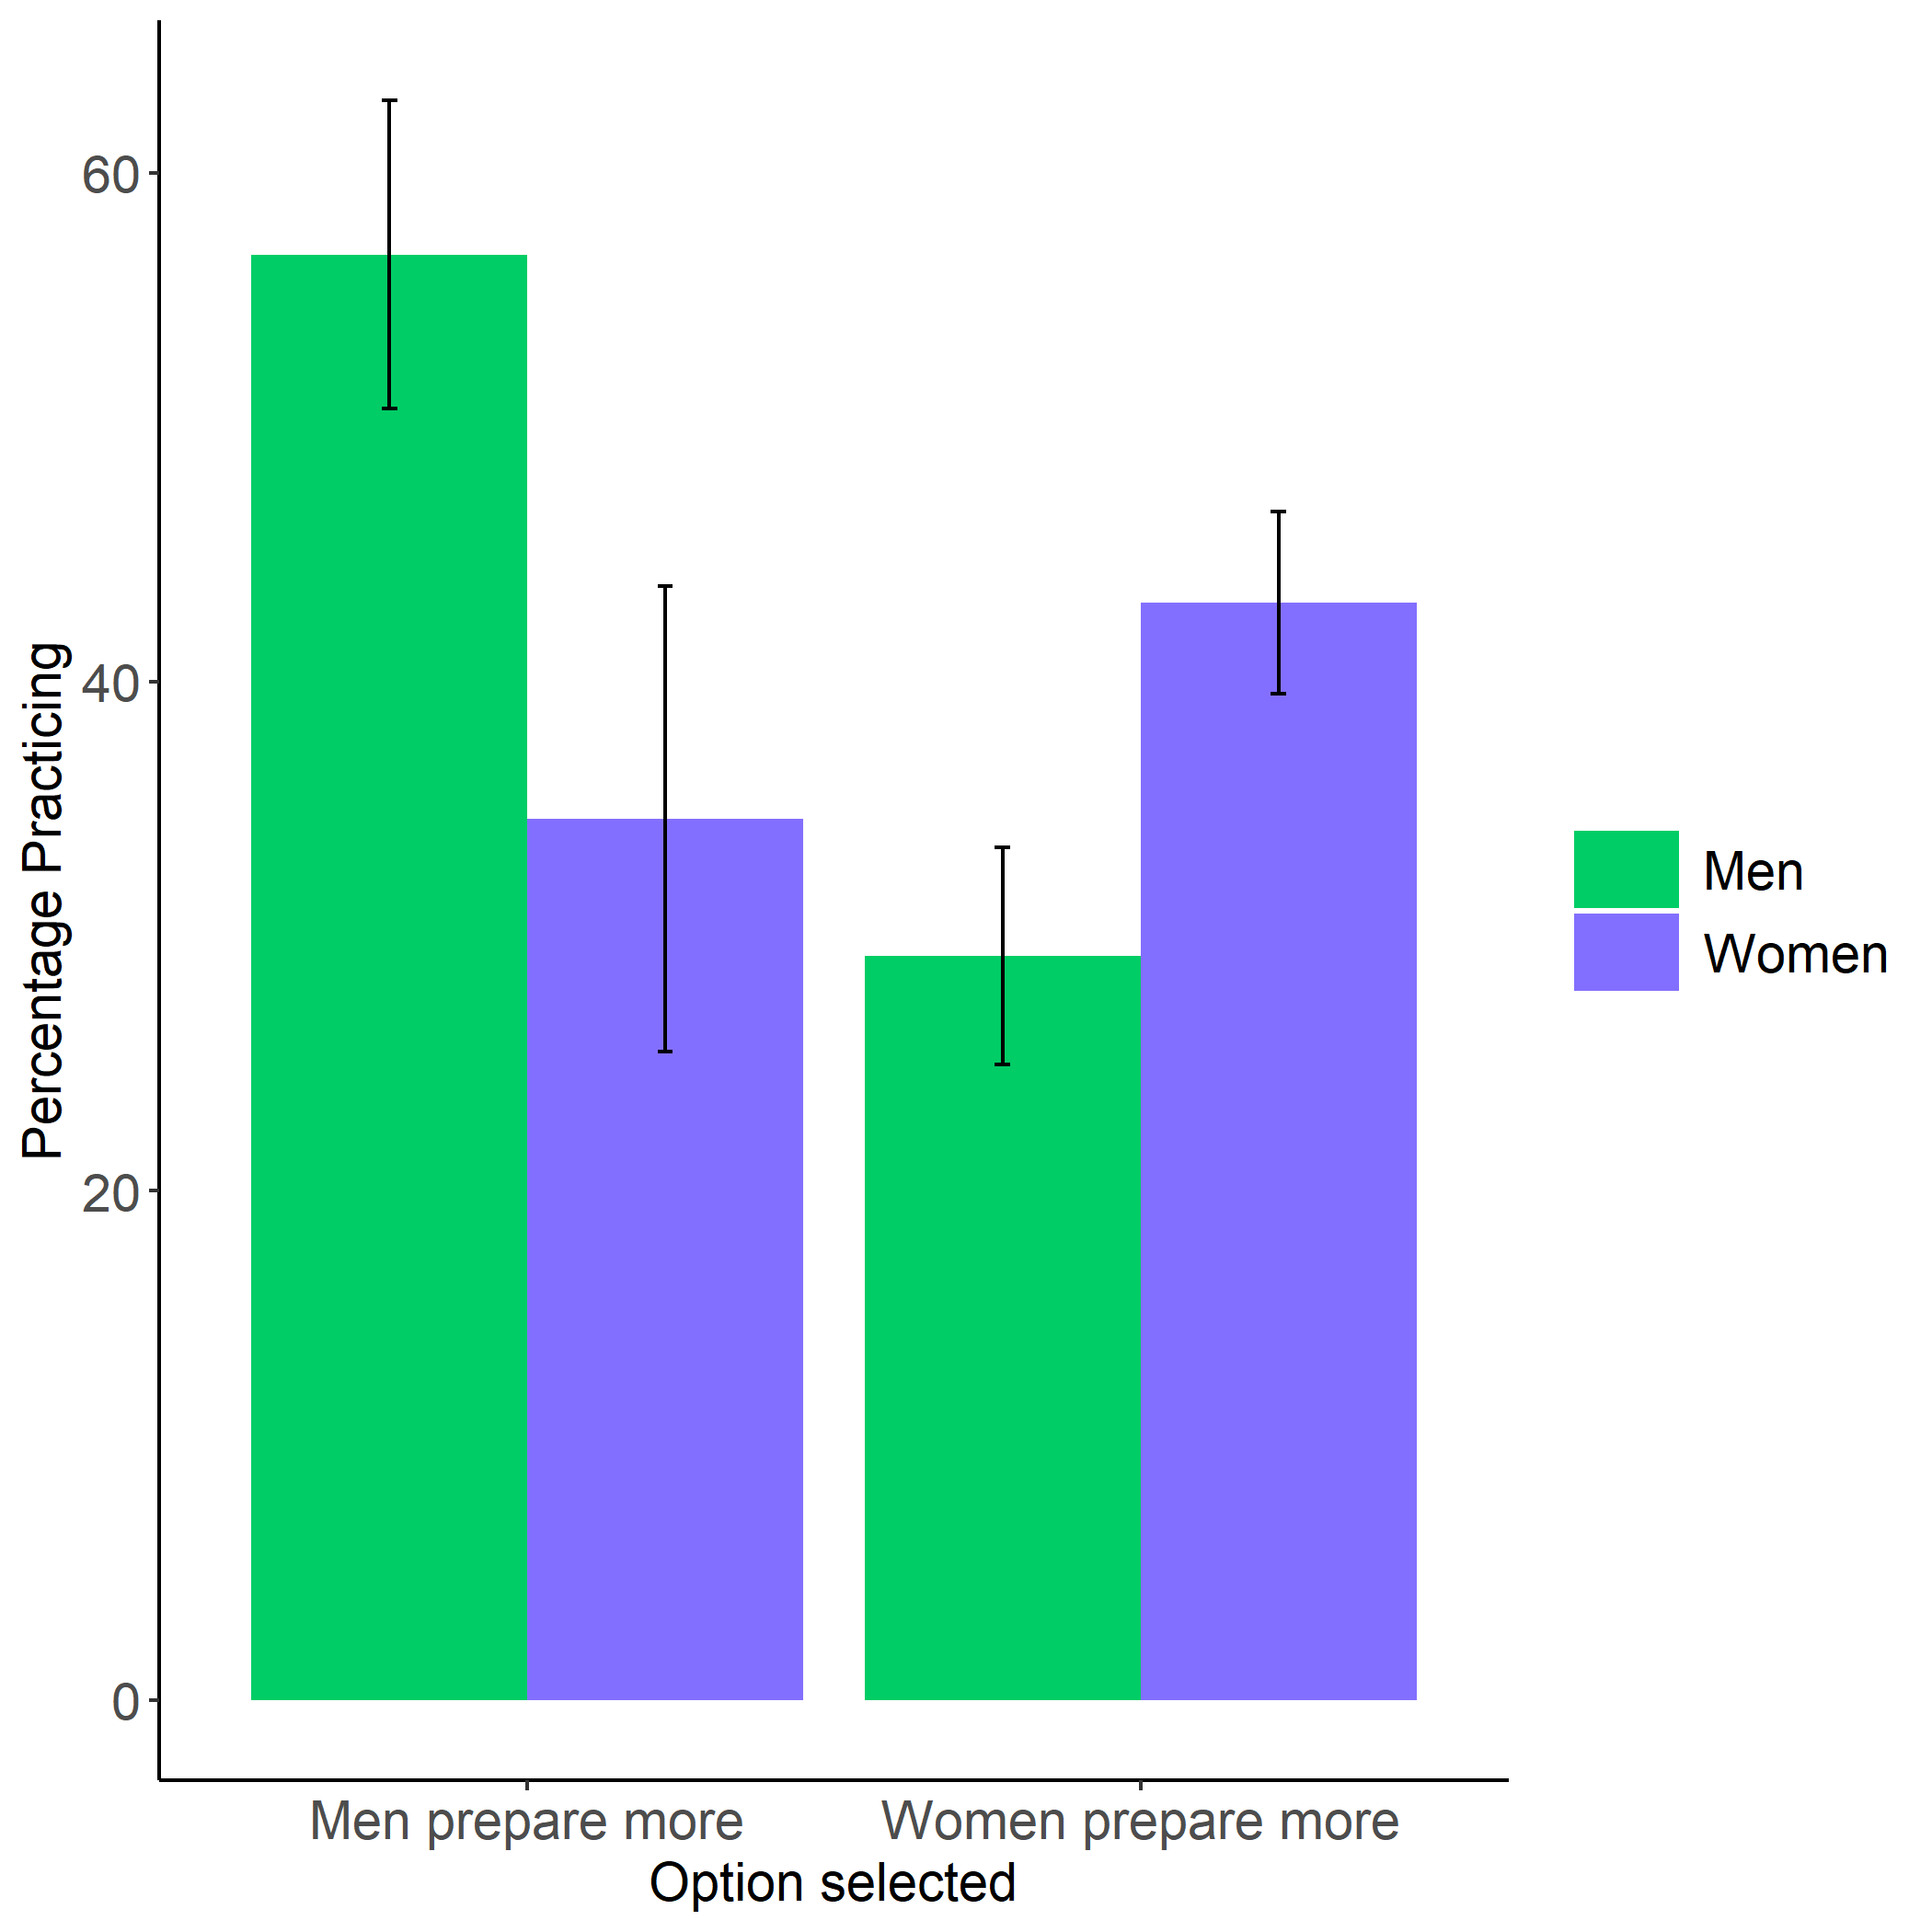
\includegraphics[width=300px]{C:/Users/keana/OneDrive - PennO365/Comp_transfer2018/Penn/practice_study/gender-practice/study2/figs/pract-choice-by-gender-and-perc-task-prep-bar-study2} 

}

\caption{Proportion of men and women in Study 2 who chose to practice based on whether they thought men or women spend more time preparing for the multiplication task. Women who thought women prepare more for the multiplication task were especially likely to choose to practice. Error bars represent standard errors.}\label{fig:pract-choice-by-gender-and-perc-task-prep-bar-study2}
\end{figure}

\hypertarget{post-manipulation-measures}{%
\subsubsection{Post-manipulation measures}\label{post-manipulation-measures}}

We also added several post-manipulation questions to tap into participants' experience of the multiplication task itself, feelings of preparedness, and general beliefs about the value of preparation to see if they may explain some of the observed effects. First, in a logistic regression with feelings of preparedness regressed upon condition and the interaction between preparation choice and gender, only the choice to prepare predicted feelings of preparation, \(b = 1.06\), 95\% CI \([0.56\), \(1.57]\), \(z = 4.14\), \(p < .001\).

We also tested whether the interaction between practice choice and condition, along with gender, predicted participants' interest in the multiplication and self-reported fatigue after completing the paid task. Our results suggest that participants who chose to prepare before the task reported feeling significantly more fatigued than those who did not choose to practice, \(b = 0.31\), 95\% CI \([0.02\), \(0.59]\), \(t(1021) = 2.08\), \(p = .038\), and that participants in the preparation condition were significantly more fatigued than those who were assigned to the control condition, \(b = 0.34\), 95\% CI \([0.08\), \(0.60]\), \(t(1021) = 2.59\), \(p = .010\). We do not find evidence that gender, \(b = -0.02\), 95\% CI \([-0.22\), \(0.18]\), \(t(1021) = -0.20\), \(p = .839\), nor the interaction between condition and practice choice, \(b = 0.17\), 95\% CI \([-0.25\), \(0.59]\), \(t(1021) = 0.78\), \(p = .433\), predicted self-reported fatigue. When gender is included as a sole predictor of self-reported fatigue, we again find no evidence that there are significant gender differences in fatigue, \(b = 0.01\), 95\% CI \([-0.20\), \(0.21]\), \(t(1024) = 0.08\), \(p = .940\). Also, we do not have evidence that gender predicted field-specific ability beliefs, \(b = -0.09\), 95\% CI \([-0.23\), \(0.05]\), \(t(1024) = -1.30\), \(p = .192\), contrary to previous work \autocite{Leslie2015}. Finally, we find that women report being significantly less interested in the task, \(b = -0.27\), 95\% CI \([-0.45\), \(-0.08]\), \(t(1021) = -2.88\), \(p = .004\), even though participants who chose to prepare tend to be significantly more interested in the task, \(b = 0.34\), 95\% CI \([0.08\), \(0.60]\), \(t(1021) = 2.61\), \(p = .009\).

\hypertarget{discussion-1}{%
\subsection{Discussion}\label{discussion-1}}

\hypertarget{summary-of-main-experimental-results-1}{%
\subsubsection{Summary of main experimental results}\label{summary-of-main-experimental-results-1}}

There is no evidence that the limited opportunity to prepare affected participants' choice to compete, nor did we find evidence of the anticipated interaction effect between gender and condition. Thus, it appears that gender differences in competitiveness are unaffected by having had the opportunity to prepare for a limited, pre-specified amount of time.

In fact, the gender difference in competitiveness itself, like in Study 1, does not hold when risk attitudes, confidence, and task scores are included in the model, suggesting the difference was explained by those variables. In this way, our study deviates from previous research suggesting that competitiveness is a stand-alone trait \autocite{Niederle2007}, and is more in line with recent evidence that competitiveness is explained by other factors (e.g., confidence or risk attitudes) \autocite{Gillen2019,Veldhuizen2017}. In line with this argument, we replicate the finding both within the broader literature and in the previous study that women are more risk averse and less confident than men. We discuss these findings across the studies of Chapter 1 in light of broader literature on whether competitiveness is a stand-alone trait further in the overall discussion section.

Contrary to Study 1, the gender differences in task scores observed when gender is included as the only predictor appear to be explained by differences in risk attitudes and confidence, since the effect of gender on task score is no longer significant when those predictors are included in the model. Thus, based on these first two sets of results, it is not entirely clear yet if there are gender differences in performance on the multiplication task used in the study.

\hypertarget{gender-differences-in-preparation-and-gender-stereotypes}{%
\subsubsection{Gender differences in preparation and gender stereotypes}\label{gender-differences-in-preparation-and-gender-stereotypes}}

Even though we do not have evidence within the context of this study that there is a gender difference in competitiveness or performance on the multiplication task when controlling for other variables, women still chose to prepare more than men - regardless of which payment scheme they ultimately selected, their risk attitudes, confidence, or task scores. At the same time, we have evidence that the choice to compete in general is related to a participants' choice to prepare, such that individuals who chose the competitive payment scheme chose to prepare at higher rates than those who chose the non-competitive payment scheme. We replicate the effects found in Study 1 when asking participants about their perceptions of these gender differences in performance, competitiveness, and preparation, such that participants were 1) significantly more likely to say that women prepare more than men both in general and on the multiplication task, despite 2) competing less and 3) performing just as well as men. Thus, we have further evidence based on participants' responses to the incentivized questions about their beliefs that there are gender stereotypes about preparation, which may in turn affect gender differences in the choice to prepare (see Section \ref{gender-stereotypes-and-practicing} for a review of the literature showing how gender stereotypes affect subsequent behavior).

On top of the gender differences in practicing and perceptions of said gender differences, we again explored whether these perceptions aligned with individuals' practicing behaviors. We find evidence that women were especially likely to prepare for the task if they believed that women prepare more than men, both in general on most tasks and specifically within the context of the multiplication task. Again, we highlight the importance of future research in testing the direction of these effects, since we cannot attest to whether perceptions lead to behavior or whether behavior leads to perceptions directly using this dataset.

\hypertarget{post-manipulation-measures-1}{%
\subsubsection{Post-manipulation measures}\label{post-manipulation-measures-1}}

Finally, we explore the new post-manipulation measures that are specific to this study. First, we find that feelings of preparedness are related to the choice to prepare. In light of the other findings, this result implies that feelings of preparedness do not derive from the required amount of preparation that one completes (that is, random assignment to condition within the context of this study), but instead, the choice to spend extra time preparing over and above what is required\footnote{Though it is worth noting that the effect of the choice to prepare may reflect the effects of variables that we are not measuring, while the random assignment to condition is estimating the causal effect of preparation on feelings of preparedness. It would be important to consider possible confounds for the effect of the choice to prepare and try to adequately capture those in future research}. Additionally, the fact that gender does not predict feelings of preparedness, despite women choosing to prepare more, has potentially important implications if replicated. That is, women may prepare more than men, yet still feel as though they are less prepared relative to others. We explore this possibility in the study of Chapter 2. These results would suggest that women's greater decisions to prepare may only contribute to feelings of preparedness that are not significantly different than men's, if they contribute at all. However, it is unclear whether the choice to prepare may be related to other variables not captured in this study that predict feelings of preparedness. Thus, future studies should explore women's and men's feelings of preparedness both before and after the choice to prepare as a way to try to address the question of what is driving the effect.

On top of the question about feelings of preparedness after completing the practice and task itself, we also asked participants to indicate their feelings about the multiplication task itself, and more specifically, how fatigued they felt after completing the task and how interested they were in the task. With regards to the question about fatigue, both participants in the limited preparation condition and participants who chose to prepare reported significantly higher levels of fatigue than participants who did not choose to prepare and were not required to. Yet, women did not report feeling significantly more fatigued than men, despite, again, choosing to prepare at significantly higher rates. Thus, women's higher rates of preparation did not seem to have negative effects on this measure attempting to capture potential negative effects of preparing. When testing effects of gender, condition, and practice choice on interest, we find that women were significantly less interested in the task, while participants who chose to prepare tended to be more interested in the task. Finally, we show that gender does not predict field-specific ability beliefs - in other words, men and women's emphasis on the importance of hard work for success (at least within the domain of math), do not appear to be significantly different in this study. This is the only study in the dissertation that includes the measures of feelings of preparedness, fatigue, and interest, and as such, replication of these results would be important to confirm they are not false positives \autocite{Coffman2015}.

\hypertarget{summary-1}{%
\subsubsection{Summary}\label{summary-1}}

Overall, we find from Study 2 of Chapter 1 that our manipulation of the limited opportunity to prepare did not reduce the gender difference in competitiveness. We show that the gender difference in competitiveness itself is explained by gender differences in risk attitudes, task scores, and confidence. Although the manipulation did not have the anticipated effects on gender differences in competitiveness, we replicate the effect that women chose to prepare more than men, which aligned with beliefs about gender differences in preparation. We also replicate the interaction effect between gender and beliefs about gender differences in preparation on the choice to prepare, again suggesting that women's preparation behaviors may have been influenced by beliefs about gender differences in preparation.

Finally, we explored participants' experiences while completing the multiplication task through questions about their feelings of preparedness, fatigue, and interest. We find that the limited preparation condition did not predict feelings of preparedness, but instead participants who chose to prepare were significantly more likely to report feeling more prepared for the multiplication task. For the measure of fatigue, participants who chose to prepare were significantly more likely to report feeling fatigued after completing the task. Finally, women were significantly less interested in the task, while participants who chose to prepare tended to be more interested in the task. Since this is the only study across all studies within this dissertation that employs these measures, and thus, we have not been able to replicate these effects, we encourage future research to ensure these effects are indeed replicable.

Since we did not find evidence that the limited opportunity to prepare affected gender differences in competitiveness, the last study in Chapter 1 tests experimentally whether having the unlimited opportunity to prepare would affect the gender gap in competitiveness. It is possible that participants in the limited preparation condition may have felt like they were not getting any additional preparation above and beyond what other participants were receiving because they could not choose how much they prepared, and thus, they did not feel like the preparation would have helped their performance substantially more than it would have helped other participants. If this possible explanation for the null effect in Study 2 is correct, we should expect to see an effect of unlimited preparation on reducing the gender difference in competitiveness.

\newpage

\hypertarget{study-3}{%
\section{Study 3}\label{study-3}}

\hypertarget{methods-2}{%
\subsection{Methods}\label{methods-2}}

\hypertarget{participants-2}{%
\subsubsection{Participants}\label{participants-2}}

All study measures described below are publicly available on OSF both as a \href{https://osf.io/yfd2j/}{.pdf} and \href{https://osf.io/vhzy5/}{.qsf}. Participants were recruited on Amazon Mechanical Turk using the same screening criteria as Studies 1 and 2. Unlike Study 2, where we filtered out second responses based on identical IP addresses, we used Qualtrics' fraud detection software to filter out responses that were suspicious either because they were likely 1) bots and/or 2) duplicate responses. For all main analyses, we excluded participants who had 1) Q\_RecaptchaScore less than .5 (indicating the respondent is likely a bot) 2) Q\_RelevantIDDuplicate equal to 1 (indicating the response is likely a duplicate) 3) Q\_RelevantIDDuplicateScore greater than or equal to 75 (indicating the response is likely a duplicate) or 4) Q\_RelevantIDFraudScore greater than or equal to 30 (indicating the response is likely fraudulent and a bot).

The final dataset consists of 1072 participants (47.2\% women), with an average age of 39.33 (\emph{SD} = 11.88) years. Of the final sample, 45 participants (44.44\% women) dropped out of the study before finishing (again, we use their data when available) and 67 participants were flagged by Qualtrics' fraud detection software as suspicious based on the aforementioned criteria.

\newpage

\begin{center}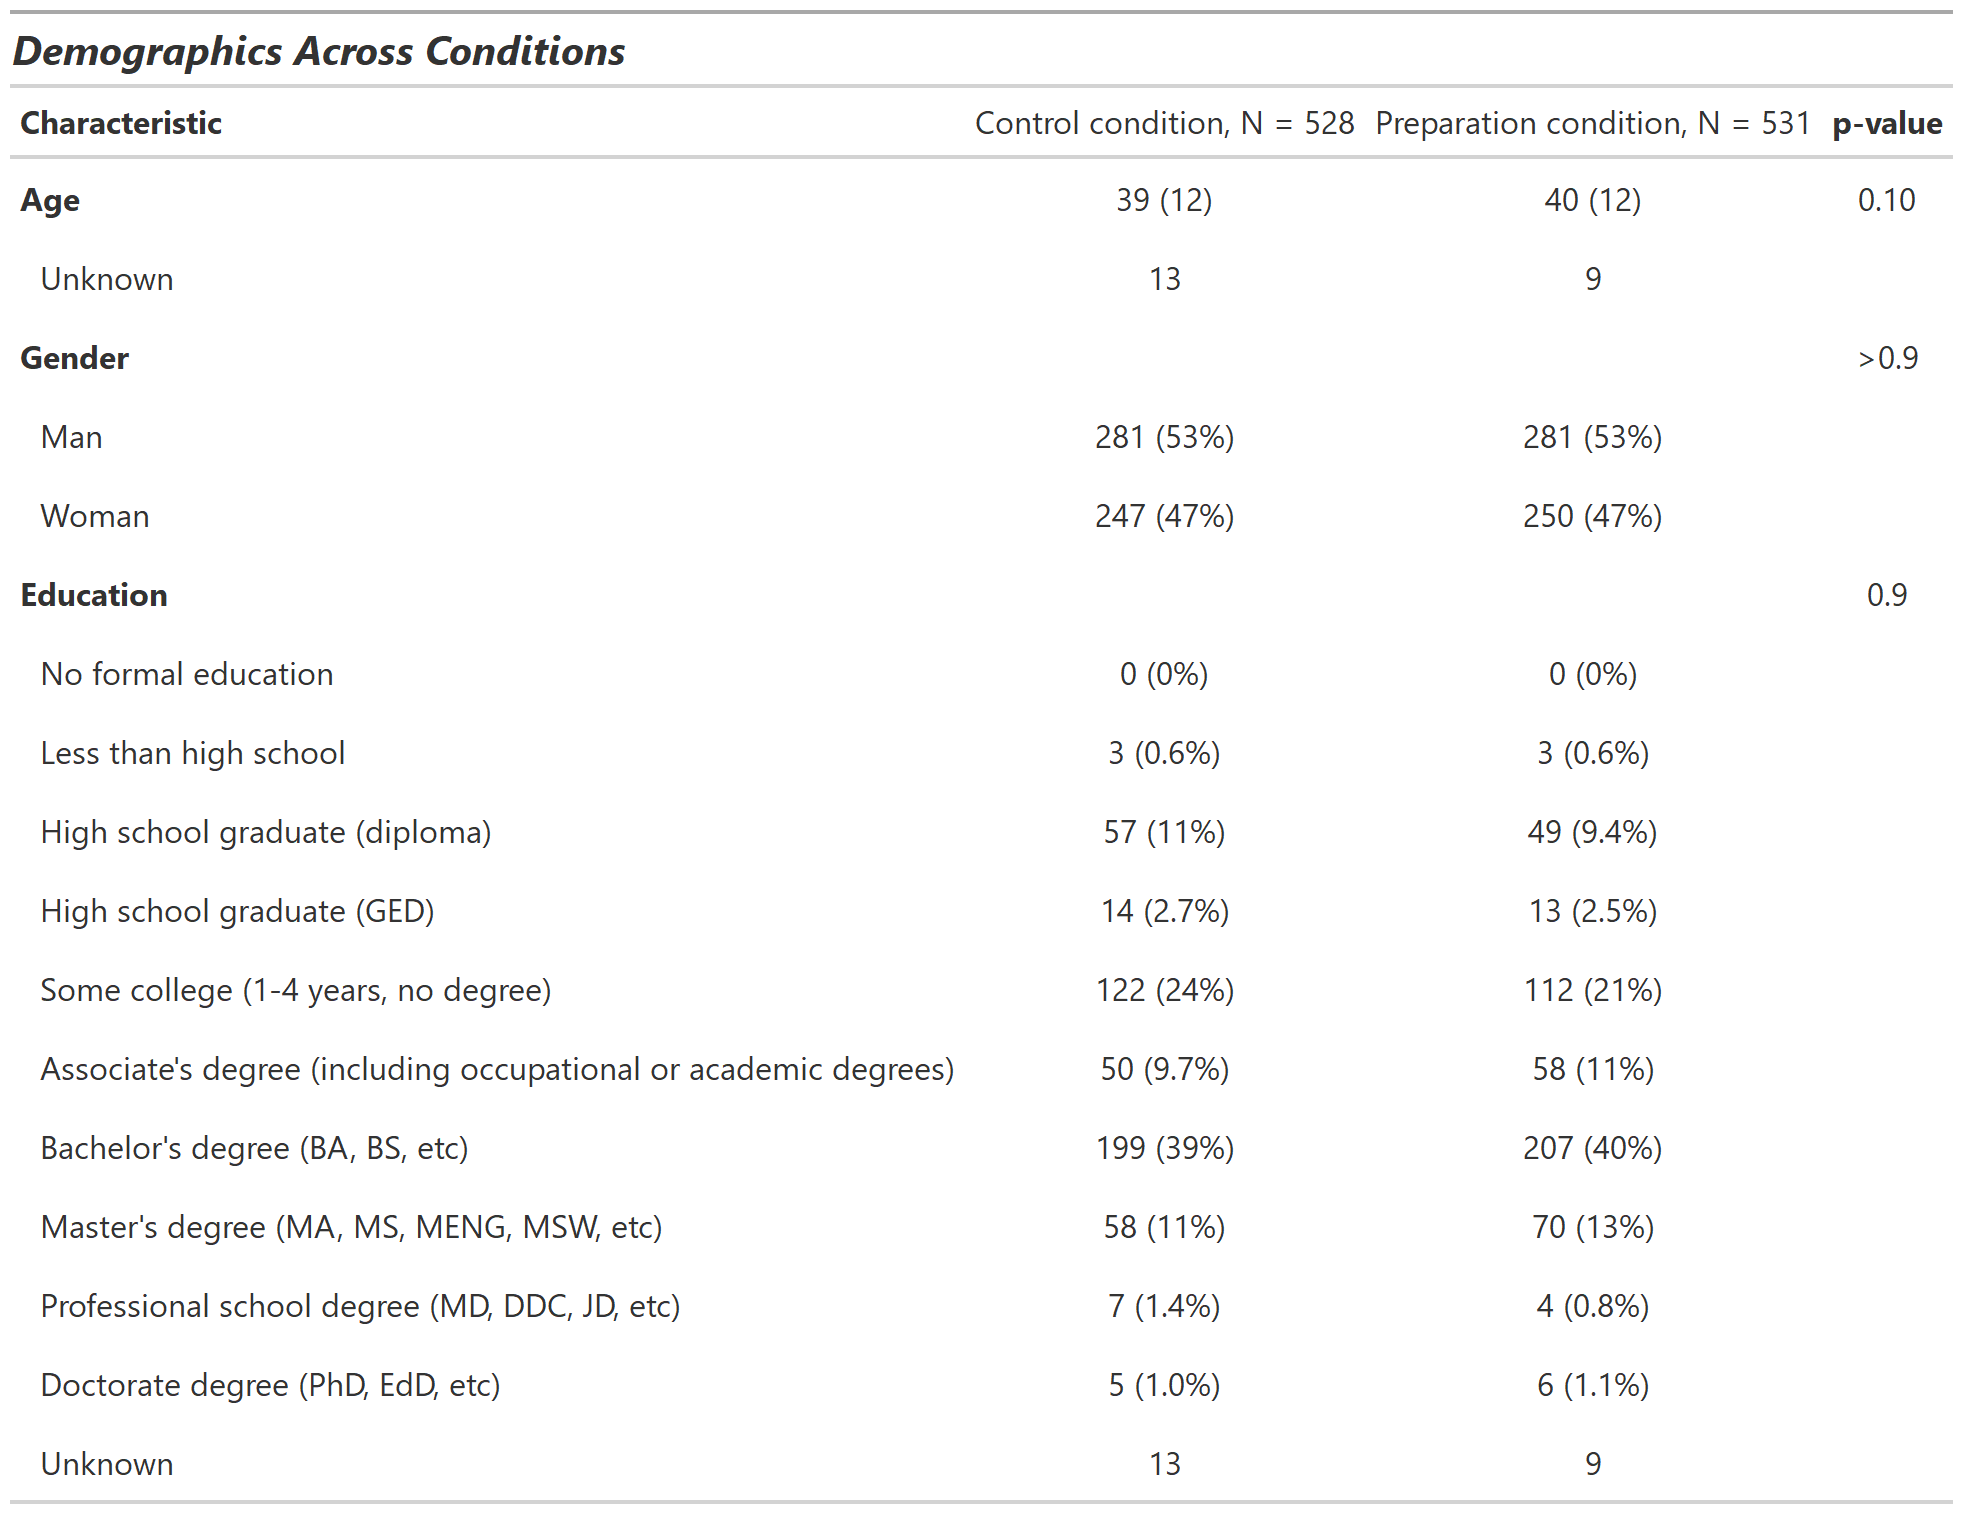
\includegraphics[width=0.85\linewidth]{C:/Users/keana/OneDrive - PennO365/Comp_transfer2018/Penn/practice_study/gender-practice/study4/figs/demographics-table-conds-study4} \end{center}

\begin{table}[ht]
\centering
\begingroup\fontsize{0.1pt}{0.1pt}\selectfont
\begin{tabular}{r}
   \\ 
 \end{tabular}
\endgroup
\caption{Size of sample in Study 3 with corresponding percentage listed for gender and education, with p-values derived from Fisher’s exact test. Mean with corresponding standard deviation listed for age, with p-values derived from Kruskal-Wallis test. If a participant did not respond to a given question, we list their response as ‘Unknown’. Note: we did not include questions about race/ethnicity nor income in this study.} 
\label{tab:demographics-table-study4}
\end{table}

\newpage

\begin{center}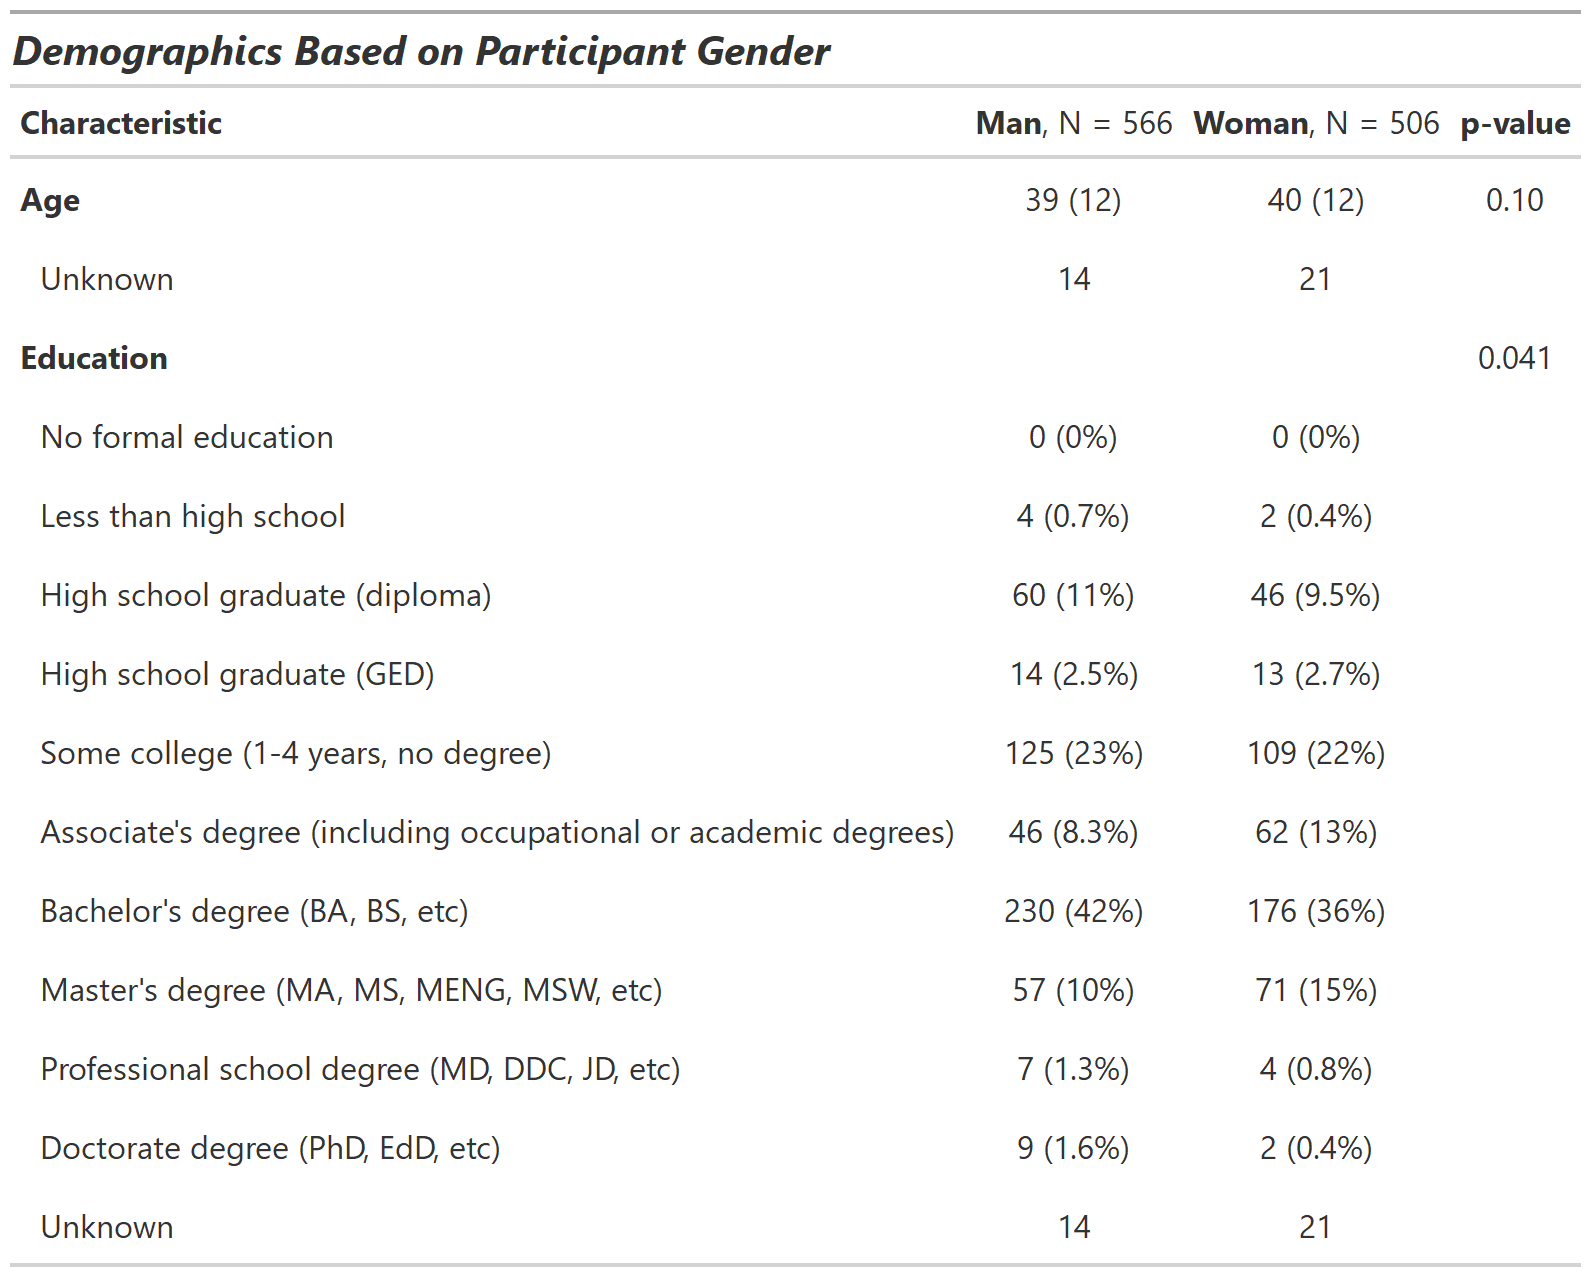
\includegraphics[width=0.85\linewidth]{C:/Users/keana/OneDrive - PennO365/Comp_transfer2018/Penn/practice_study/gender-practice/study4/figs/demographics-table-gender-study4} \end{center}

\begin{table}[ht]
\centering
\begingroup\fontsize{0.1pt}{0.1pt}\selectfont
\begin{tabular}{r}
   \\ 
 \end{tabular}
\endgroup
\caption{Size of sample in Study 3 with corresponding percentage listed for education, with p-values derived from Fisher’s exact test. Mean with corresponding standard deviation listed for age, with p-values derived from Kruskal-Wallis test. If a participant did not respond to a given question, we list their response as ‘Unknown’. Note: we did not include questions about race/ethnicity nor income in this study.} 
\label{tab:demographics-table-gender-study4}
\end{table}

\hypertarget{procedures-2}{%
\subsubsection{Procedures}\label{procedures-2}}

As in Studies 1 and 2, participants included in the study were told they would be completing a two-minute multiplication task (identical to the ones used in previous studies) and would be able to choose a payment scheme for their performance. After being told about the rules for the multiplication task and passing the same comprehension questions used in the previous studies, participants were assigned to either an unlimited preparation condition, where they could complete as many practice multiplication problems as they wanted, with the option to opt out of the practice at any time before moving on to the multiplication task, or a control condition, where they were told they could complete as many rounds of a subtraction exercise as they wanted before the multiplication task. An equal number of participants were randomly assigned to both conditions (control= 49.86\%), with no significant difference in representation of men and women across conditions, \(\chi^2(1, n = 1072) = 0.00\), \(p = .971\), confirming there was random assignment to conditions based on gender. Participants across both conditions were given the option to study the multiplication (preparation condition) or subtraction (control condition) tables for as long as they wanted. We measured both the decision to study the respective table within each condition, along with the amount of time that participants who chose to study the tables spent on that page. Next, participants within each condition were given the option to complete problems from the tables within their respective condition. Problems were created by randomly drawing pairs of numbers from 1 to 12 and asking participants to multiply them together (preparation condition) or subtract them (control condition). Participants across both conditions were able to complete 10 problems at a time before being prompted to indicate whether they would like to continue completing problems. Like the previous studies, we measured the decision to practice multiplication problems (or in the case of the control condition, complete subtraction problems), along with the number of rounds of practice participants completed. Here, the number of rounds of practice was encoded as follows: participants who did not choose to practice had a value of zero for this variable, participants who chose to practice had a value of one for this variable, and thereafter the variable increased incrementally in correspondence with each round of practice participants completed. This variable had a mean of 0.33, with an \emph{SD} of 1.03.

Afterwards, all participants chose a payment scheme for the multiplication task, described and counterbalanced in the same way as in Studies 1 and 2. Then, participants completed the paid multiplication task for two minutes. We included many of the same follow-up questions as in Studies 1 and 2, including measures of risk attitudes, confidence, perceptions of gender differences in preparation on the multiplication task (for participants in the preparation condition), perceptions of gender differences in preparation in general, competitiveness, and performance. Notably, we added in an additional response option for all of the questions about perceptions of gender differences in behavior, such that participants in this study could choose between saying men were more likely to engage in the specified behavior, women were more likely to engage in the specified behavior, or that there would be no gender differences in the specified behavior. Like before, participants were incentivized to answer the questions about their confidence and perceptions of gender differences correctly, and were paid at the same rate as Studies 1 and 2. Participants also completed a manipulation check, where they were told about the two conditions, and were asked which of the conditions they thought was more helpful in boosting scores on the paid multiplication task. Finally, they completed some demographic questions and provided feedback on the study before being paid for their participation.

\hypertarget{results-2}{%
\subsection{Results}\label{results-2}}

\hypertarget{describing-main-variables-of-interest-2}{%
\subsubsection{Describing main variables of interest}\label{describing-main-variables-of-interest-2}}

We start by exploring gender differences across the main variables of interest to compare the characteristics of our sample to previous samples in the literature and provide context for the subsequent analyses. First, we replicated the effect from the previous studies of gender on the choice to compete when gender is included as the only predictor in the logistic regression: 20.22\% of men chose to compete compared to 8.85\% of women, \(b = -0.96\), 95\% CI \([-1.34\), \(-0.59]\), \(z = -5.01\), \(p < .001\). However, like the previous two studies, when running regressions including control variables (i.e., task score, risk attitudes, confidence, and the interaction between gender and condition), we find that the effect of gender on the choice to compete is not significant, \(b = -0.15\), 95\% CI \([-0.69\), \(0.37]\), \(z = -0.56\), \(p = .573\), suggesting the effect is explained fully by risk attitudes, \(b = 0.33\), 95\% CI \([0.25\), \(0.41]\), \(z = 7.79\), \(p < .001\), task score, \(b = 0.02\), 95\% CI \([0.01\), \(0.03]\), \(z = 3.84\), \(p < .001\), and confidence, \(b = 0.01\), 95\% CI \([0.00\), \(0.02]\), \(z = 2.17\), \(p = .030\) (See Table \ref{tab:tab-comp-choice-study4}). On the other hand, we replicate effects from the literature of gender on both confidence, \(b = -14.06\), 95\% CI \([-16.73\), \(-11.39]\), \(t(1035) = -10.35\), \(p < .001\), and risk attitudes, \(b = -1.02\), 95\% CI \([-1.33\), \(-0.71]\), \(t(1035) = -6.48\), \(p < .001\), where women tend to be less confident with regards to their performance on the task and generally more risk averse relative to men.

\begin{center}
\includegraphics[width=1\linewidth]{C:/Users/keana/OneDrive - PennO365/Comp_transfer2018/Penn/practice_study/gender-practice/study4/figs/tab_comp-choice-study4} \end{center}

\begin{table}[ht]
\centering
\begingroup\fontsize{0.1pt}{0.1pt}\selectfont
\begin{tabular}{r}
   \\ 
 \end{tabular}
\endgroup
\caption{All models are logistic regressions with choice to compete as the dependent variable, where man and control are the reference categories for participant gender and preparation condition, respectively. The gender difference in the choice to compete is not reduced by preparation condition, but is explained by risk attitudes, confidence, and task scores. p < .05 is considered significant and bolded.} 
\label{tab:tab-comp-choice-study4}
\end{table}

Another important consideration when interpreting any main effects found in this study is whether there are gender differences in task scores. When including gender by itself as a predictor of performance, we find that women have significantly lower task scores, \(b = -7.60\), 95\% CI \([-10.07\), \(-5.12]\), \(t(1035) = -6.01\), \(p < .001\). However, when controlling for competition choice, confidence, and risk attitudes, the effect of gender is not significant, \(b = -1.35\), 95\% CI \([-3.79\), \(1.09]\), \(t(1031) = -1.09\), \(p = .278\), suggesting that these variables explain the gender difference in task scores. Specifically, we find that both confidence, \(b = 0.43\), 95\% CI \([0.38\), \(0.49]\), \(t(1031) = 16.84\), \(p < .001\), and competition choice, \(b = 8.23\), 95\% CI \([4.42\), \(12.03]\), \(t(1031) = 4.24\), \(p < .001\), positively predict task scores (that is, those who are more confident and chose to compete tend to have higher task scores), while risk attitudes negatively predict task scores (that is, individuals who are more risk seeking tend to have lower scores), \(b = -1.14\), 95\% CI \([-1.58\), \(-0.69]\), \(t(1031) = -4.98\), \(p < .001\) (See Table \ref{tab:tab-task-scores-study4}). See Table \ref{tab:summary-table-gender-study4} for a summary of gender differences in the main variables of interest.

\begin{center}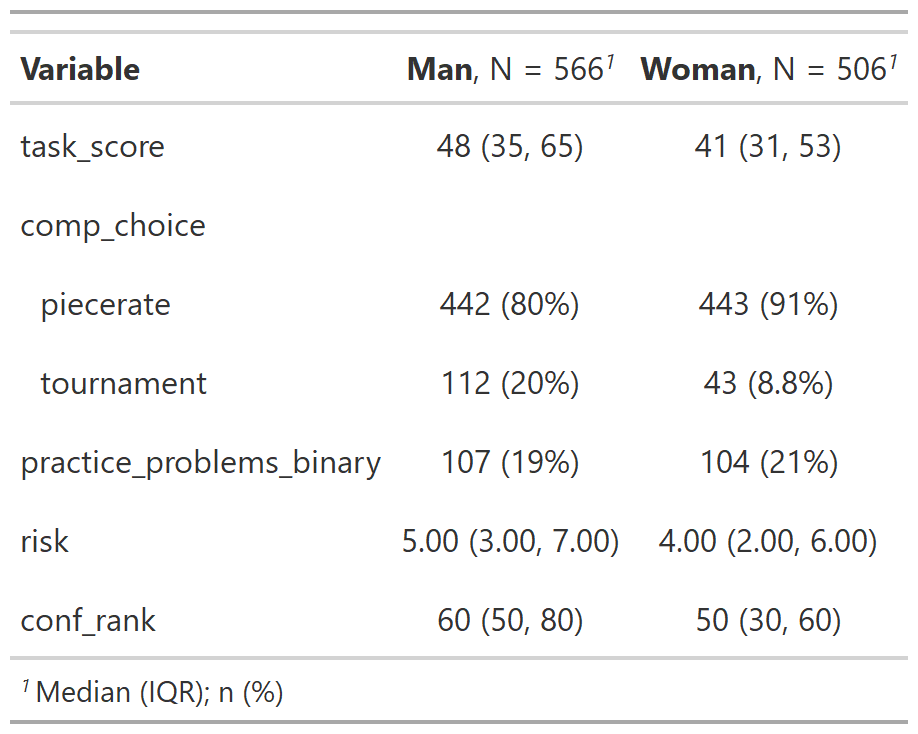
\includegraphics[width=0.5\linewidth]{C:/Users/keana/OneDrive - PennO365/Comp_transfer2018/Penn/practice_study/gender-practice/study4/figs/summary-table-gender-study4} \end{center}

\begin{table}[ht]
\centering
\begingroup\fontsize{0.1pt}{0.1pt}\selectfont
\begin{tabular}{r}
   \\ 
 \end{tabular}
\endgroup
\caption{Gender differences in the main variables of interest, including: task scores, choice to compete, choice to practice (among the full dataset), confidence, and risk attitudes. Medians are reported for task score, risk attitudes, and confidence, with IQRs in parentheses. For choice to practice and choice to compete, we report the number and percentage of participants that fall into each category for each respective gender.} 
\label{tab:summary-table-gender-study4}
\end{table}

\newpage

\begin{center}
\includegraphics[width=1\linewidth]{C:/Users/keana/OneDrive - PennO365/Comp_transfer2018/Penn/practice_study/gender-practice/study4/figs/tab_task-scores-study4} \end{center}

\begin{table}[ht]
\centering
\begingroup\fontsize{0.1pt}{0.1pt}\selectfont
\begin{tabular}{r}
   \\ 
 \end{tabular}
\endgroup
\caption{All models are linear regressions with task score as the dependent variable, where man and piece-rate payment scheme are the reference categories for participant gender and competition choice, respectively. After controlling for risk attitudes, confidence, and competition choice, women no longer have lower scores on the multiplication task than men, p < .05 is considered significant and bolded.} 
\label{tab:tab-task-scores-study4}
\end{table}

\hypertarget{effects-of-unlimited-preparation-condition-on-gender-differences-in-choice-to-compete}{%
\subsubsection{Effects of unlimited preparation condition on gender differences in choice to compete}\label{effects-of-unlimited-preparation-condition-on-gender-differences-in-choice-to-compete}}

We do not find evidence of a significant effect of preparing with multiplication or subtraction problems (task relevant vs.~irrelevant preparation condition) on the choice to compete across all participants, \(b = -0.33\), 95\% CI \([-0.68\), \(0.01]\), \(z = -1.88\), \(p = .061\) when included as a single predictor of the choice to compete in a logistic regression. The point estimate for the effect of the unlimited preparation condition was negative and the 95\% CI did not include positive effects that were greater in magnitude than 0.01. In a subsequent logistic regression adding in gender and the interaction between gender and condition as predictors, we find that gender is the only significant predictor of the choice to compete, \(b = -0.68\), 95\% CI \([-1.18\), \(-0.21]\), \(z = -2.77\), \(p = .006\) and no evidence of the expected interaction effect between gender and condition on the choice to compete, \(b = -0.68\), 95\% CI \([-1.48\), \(0.09]\), \(z = -1.70\), \(p = .089\) (see Figure \ref{fig:s300}).\footnote{The interaction between gender and preparation condition on the choice to compete is still not significant among the full dataset (i.e., after including participants that were flagged by Qualtrics' fraud detection software): \(b = -0.54\), 95\% CI \([-1.27\), \(0.18]\), \(z = -1.45\), \(p = .148\)}

\begin{figure}

{\centering 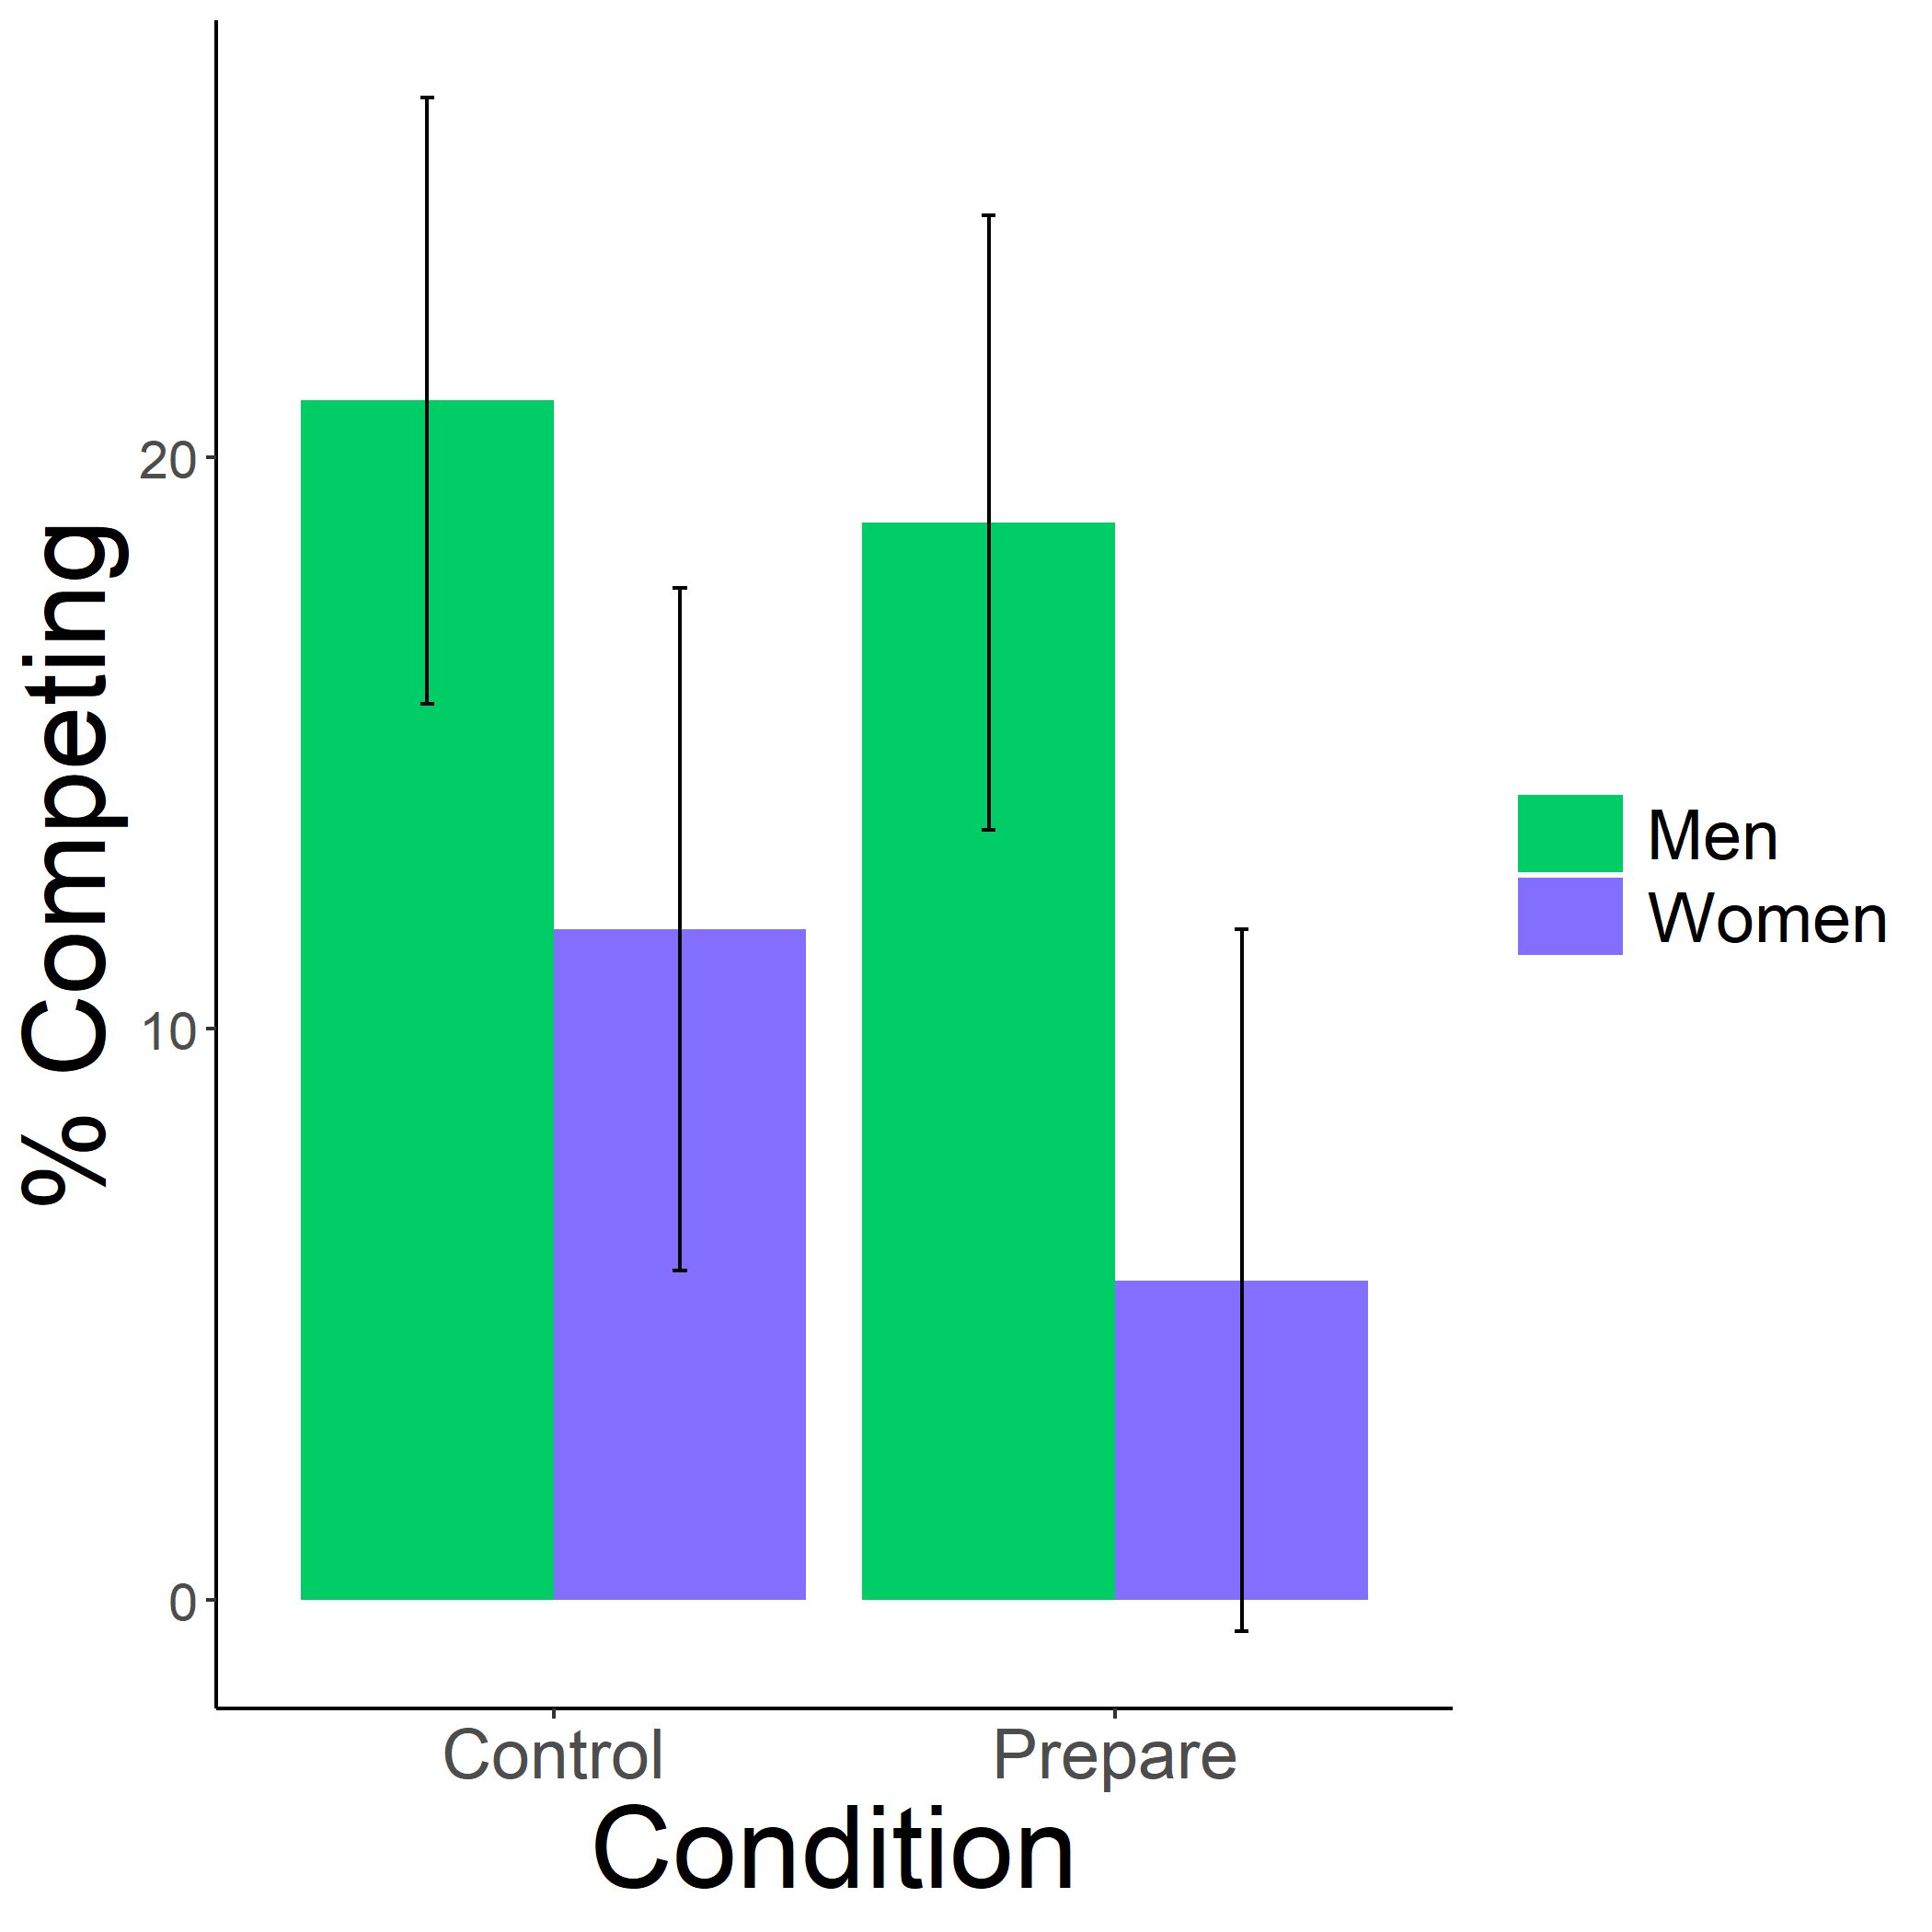
\includegraphics[width=300px]{C:/Users/keana/OneDrive - PennO365/Comp_transfer2018/Penn/practice_study/gender-practice/study4/figs/fig02_comp-choice-by-gender-and-cond-bar} 

}

\caption{Proportion of men and women in Study 3 who chose to compete based on preparation condition. Unlimited preparation did not reduce the gender difference in competitiveness. Error bars represent standard errors.}\label{fig:s300}
\end{figure}

\newpage

\hypertarget{gender-differences-in-preparation-3}{%
\subsubsection{Gender differences in preparation}\label{gender-differences-in-preparation-3}}

Our next set of analyses focused on the effects of gender on decisions to practice. Thus, all subsequent analyses focus on the subset of participants that were assigned to the unlimited preparation condition that were actually given the opportunity to practice beforehand (N = 571). We do not replicate the effect found in both previous studies of gender on the decision to practice multiplication problems, neither in the model where gender is included by itself as a sole predictor of the choice to practice, \(b = 0.11\), 95\% CI \([-0.27\), \(0.50]\), \(z = 0.58\), \(p = .565\) (see right panel of Figure \ref{fig:panel-study4}), nor in tandem with the choice to compete and the interaction between gender and the choice to compete as predictors, \(b = 0.34\), 95\% CI \([-0.09\), \(0.77]\), \(z = 1.55\), \(p = .121\) (see left panel of Figure \ref{fig:panel-study4}).\footnote{The effect of gender on the choice to prepare is still not significant among the full dataset (i.e., after including participants that were flagged by Qualtrics' fraud detection software): \(b = 0.12\), 95\% CI \([-0.25\), \(0.50]\), \(z = 0.64\), \(p = .519\)} Though the effect is not significant, the proportion of women that chose to practice was still higher than the proportion of men that chose to practice (26.87\% of women chose to prepare via practice, relative to 24.5\% of men) among participants within the unlimited practice condition. Thus, the direction of the effects are not in contrast with previous studies. In line with the previous studies, we do not find an interaction between gender and choice to compete on the choice to practice, \(b = -1.22\), 95\% CI \([-2.84\), \(0.15]\), \(z = -1.64\), \(p = .101\). Instead we find that, like previous studies, the choice to compete is positively related to the choice to practice, \(b = 0.88\), 95\% CI \([0.23\), \(1.51]\), \(z = 2.70\), \(p = .007\). In adding confidence and risk attitudes as predictors to the model with the interaction effect on top of the main effects, we do not find evidence that either of those predictors are significantly related to the choice to practice either (See Table \ref{tab:tab-pract-choice-study4}). Like the previous two studies in Chapter 1, we also ran a two-part hurdle model with gender, competition choice, and the interaction between those variables predicting the number of practice rounds variable (among participants in the practice condition) and again do not find evidence of gender differences in the choice to continue preparing after the initial decision to prepare, , \emph{b} = 0.42, 95\% CI {[}-0.31, 1.15{]}, \emph{z} = 1.14, \emph{p} = 0.25. Unlike the previous studies, this study separated the decision to study tables and amount of time studying tables from the decision to practice and number of problems completed, so we had the novel opportunity to explore questions about gender differences in studying here. We do not find evidence that there are gender differences in the decision to study the multiplication tables, \(b = 0.09\), 95\% CI \([-0.28\), \(0.47]\), \(z = 0.49\), \(p = .624\). However, among participants who did choose to study the multiplication tables (N = 234; 40.98\% of participants in the unlimited preparation condition), we find that women studied for more time (in seconds) than men on average, M\textsubscript{women} =33.01, SD\textsubscript{women} =72.74; M\textsubscript{men}= 18.75, SD\textsubscript{men} =25.24, \(b = 21.94\), 95\% CI \([2.65\), \(41.23]\), \(t(211) = 2.24\), \(p = .026\).\footnote{However, we note that the SD for studying time among women is exceptionally high relative to that of men, so the effect may be driven by select outliers pulling the mean}

\begin{figure}

{\centering 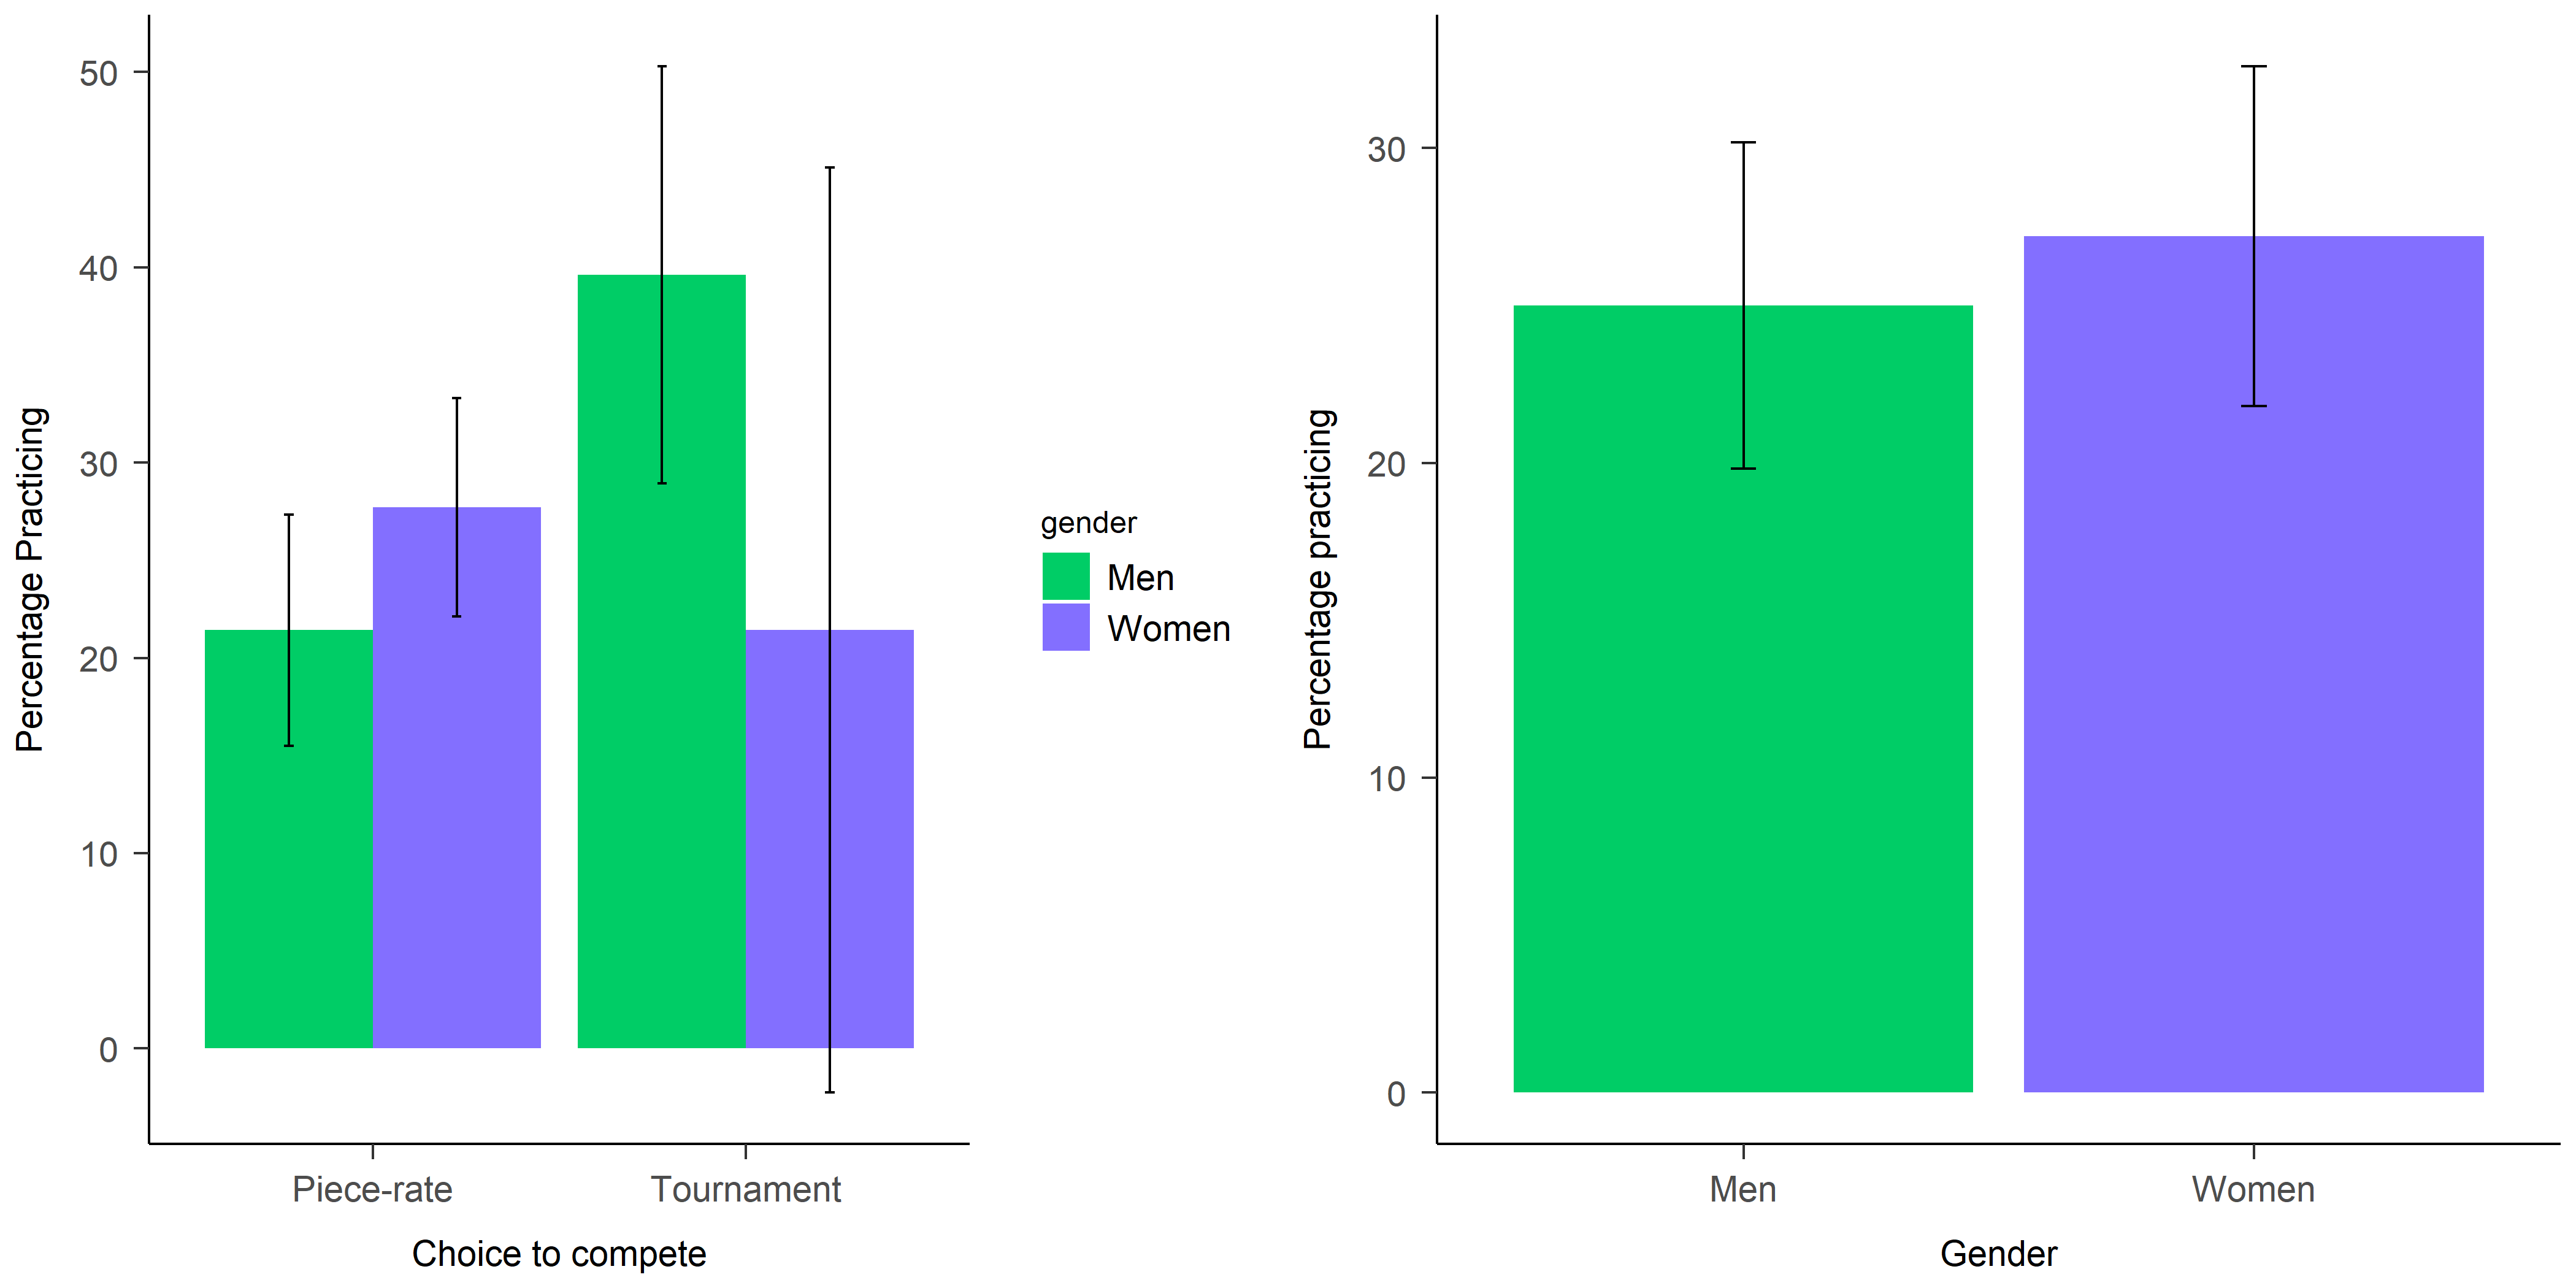
\includegraphics[width=1\linewidth]{C:/Users/keana/OneDrive - PennO365/Comp_transfer2018/Penn/practice_study/gender-practice/study4/figs/panel_study4} 

}

\caption{Right panel shows the proportion of men and women in Study 3 who chose to prepare. Left panel shows the proportion of men and women in Study 3 who chose to prepare based on choice to compete. Error bars represent standard errors.}\label{fig:panel-study4}
\end{figure}

\newpage

\begin{center}
\includegraphics[width=1\linewidth]{C:/Users/keana/OneDrive - PennO365/Comp_transfer2018/Penn/practice_study/gender-practice/study4/figs/tab_pract-choice-study4} \end{center}

\begin{table}[ht]
\centering
\begingroup\fontsize{0.1pt}{0.1pt}\selectfont
\begin{tabular}{r}
   \\ 
 \end{tabular}
\endgroup
\caption{All models are logistic regressions with choice to prepare as the dependent variable, where man and piece-rate payment scheme are the reference categories for participant gender and competition choice, respectively. We do not find evidence that women prepare more than men. p < .05 is considered significant and bolded.} 
\label{tab:tab-pract-choice-study4}
\end{table}

\hypertarget{perceptions-of-gender-differences-in-preparation-performance-and-competitiveness-3}{%
\subsubsection{Perceptions of gender differences in preparation, performance, and competitiveness}\label{perceptions-of-gender-differences-in-preparation-performance-and-competitiveness-3}}

Like all studies before, for each question about perceptions of gender differences, we run a chi-square goodness of fit test with the null hypothesis that participants' will choose each option at a similar rate. Since participants were given the option in this study to select one of three response options, rather than two options like the first two studies, we first perform a chi-square goodness of fit test with all response options to see if they are all equally likely. If the test with all three response options was significant, we then performed more targeted chi-square goodness of fit tests with pairs of response options within a given question to test which specific pairs of response options are significantly different. See Table \ref{tab:summary-table-beliefs-study4} for a summary of participants' responses to the questions about gender differences in preparation, performance, and competitiveness.

When asked to predict gender differences in preparation for the multiplication task,\footnote{Note: this question was only asked among participants in the preparation condition} we find that participants' responding is not evenly distributed across the response options, \(\chi^2(2, n = 571) = 192.97\), \(p < .001\). In performing more targeted analyses, we find that participants were significantly more likely to choose ``women'' (56.7\%) than ``men'' (7.28\%), \(\chi^2(1, n = 571) = 199.29\), \(p < .001\), or ``no difference'' (36.02\%), \(\chi^2(1, n = 571) = 24.10\), \(p < .001\) in response to this question (see Figure \ref{fig:s303}).

This result replicates when participants are asked about gender differences in general tendencies to prepare, \(\chi^2(2, n = 1072) = 358.38\), \(p < .001\) (see Figure \ref{fig:s306}), such that, across all participants, a significantly higher proportion of participants said women prepare more in general (59.5\%) than the proportion of participants that said men prepare more (12.34\%), \(\chi^2(1, n = 1072) = 320.97\), \(p < .001\), or there are no gender differences in general tendencies to prepare (28.16\%), \(\chi^2(1, n = 1072) = 116.20\), \(p < .001\).

Though participants consistently expected women to be more likely to prepare than men, they did not expect that there would be a gender difference in performance, \(\chi^2(2, n = 1072) = 77.76\), \(p < .001\) (see Figure \ref{fig:s304}), where participants were significantly more likely to indicate ``no difference'' (46.09\%) compared to ``men'' (28.64\%), \(\chi^2(1, n = 1072) = 42.27\), \(p < .001\), or ``women'' (25.27\%), \(\chi^2(1, n = 1072) = 63.05\), \(p < .001\), in response to this question.

Despite thinking that there would be no gender difference in performance and expecting women to prepare for the task more, participants consistently expected men to be more likely to compete (78.01\%), \(\chi^2(2, n = 1072) = 961.58\), \(p < .001\) (see Figure \ref{fig:s305}), rather than expecting women to compete more (4.05\%), \(\chi^2(1, n = 1072) = 691.29\), \(p < .001\), or expecting no difference in willingness to compete across genders, (17.94\%), \(\chi^2(1, n = 1072) = 390.08\), \(p < .001\). We discuss these findings about participants' beliefs in light of the actual study results in the discussion section.

\begin{center}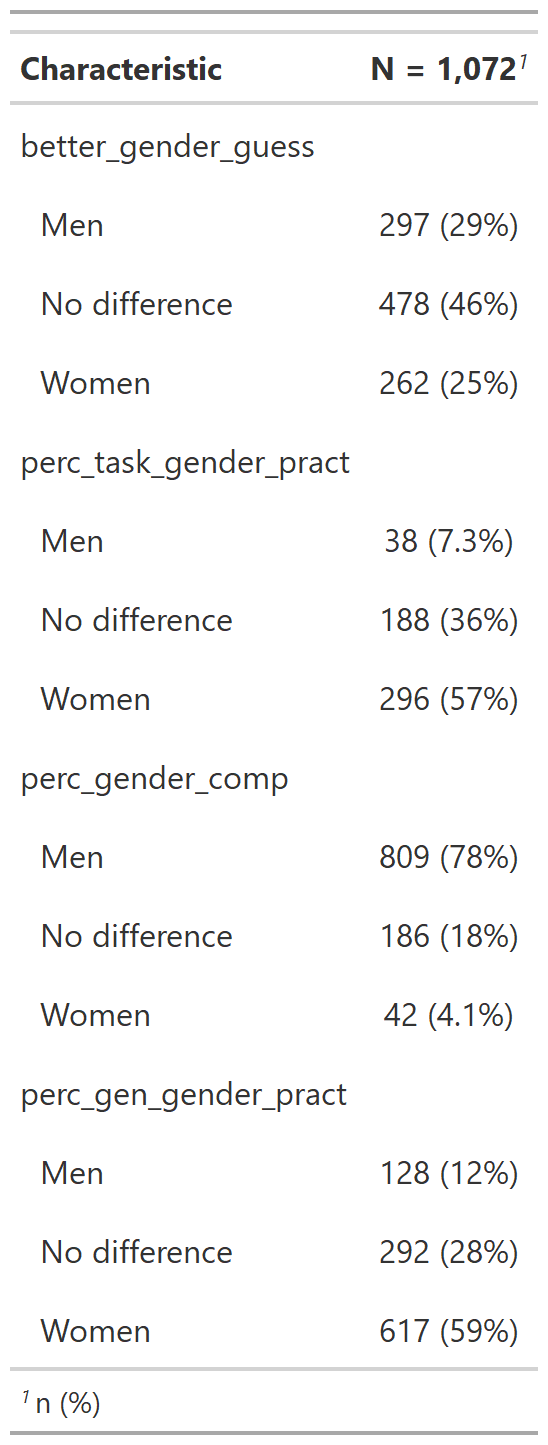
\includegraphics[width=0.35\linewidth]{C:/Users/keana/OneDrive - PennO365/Comp_transfer2018/Penn/practice_study/gender-practice/study4/figs/summary-table-beliefs-study4} \end{center}

\begin{table}[ht]
\centering
\begingroup\fontsize{0.1pt}{0.1pt}\selectfont
\begin{tabular}{r}
   \\ 
 \end{tabular}
\endgroup
\caption{Number and percentage of participants that selected each respective option when asked whether men or women would correctly solve more problems on the multiplication task, spend more time preparing for the multiplication task, choose the tournament payment scheme more often, and spend more time preparing on most tasks. Participants were also given the option in this study to indicate there would be no gender difference for any of the variables.} 
\label{tab:summary-table-beliefs-study4}
\end{table}

\newpage
\begin{figure}

{\centering 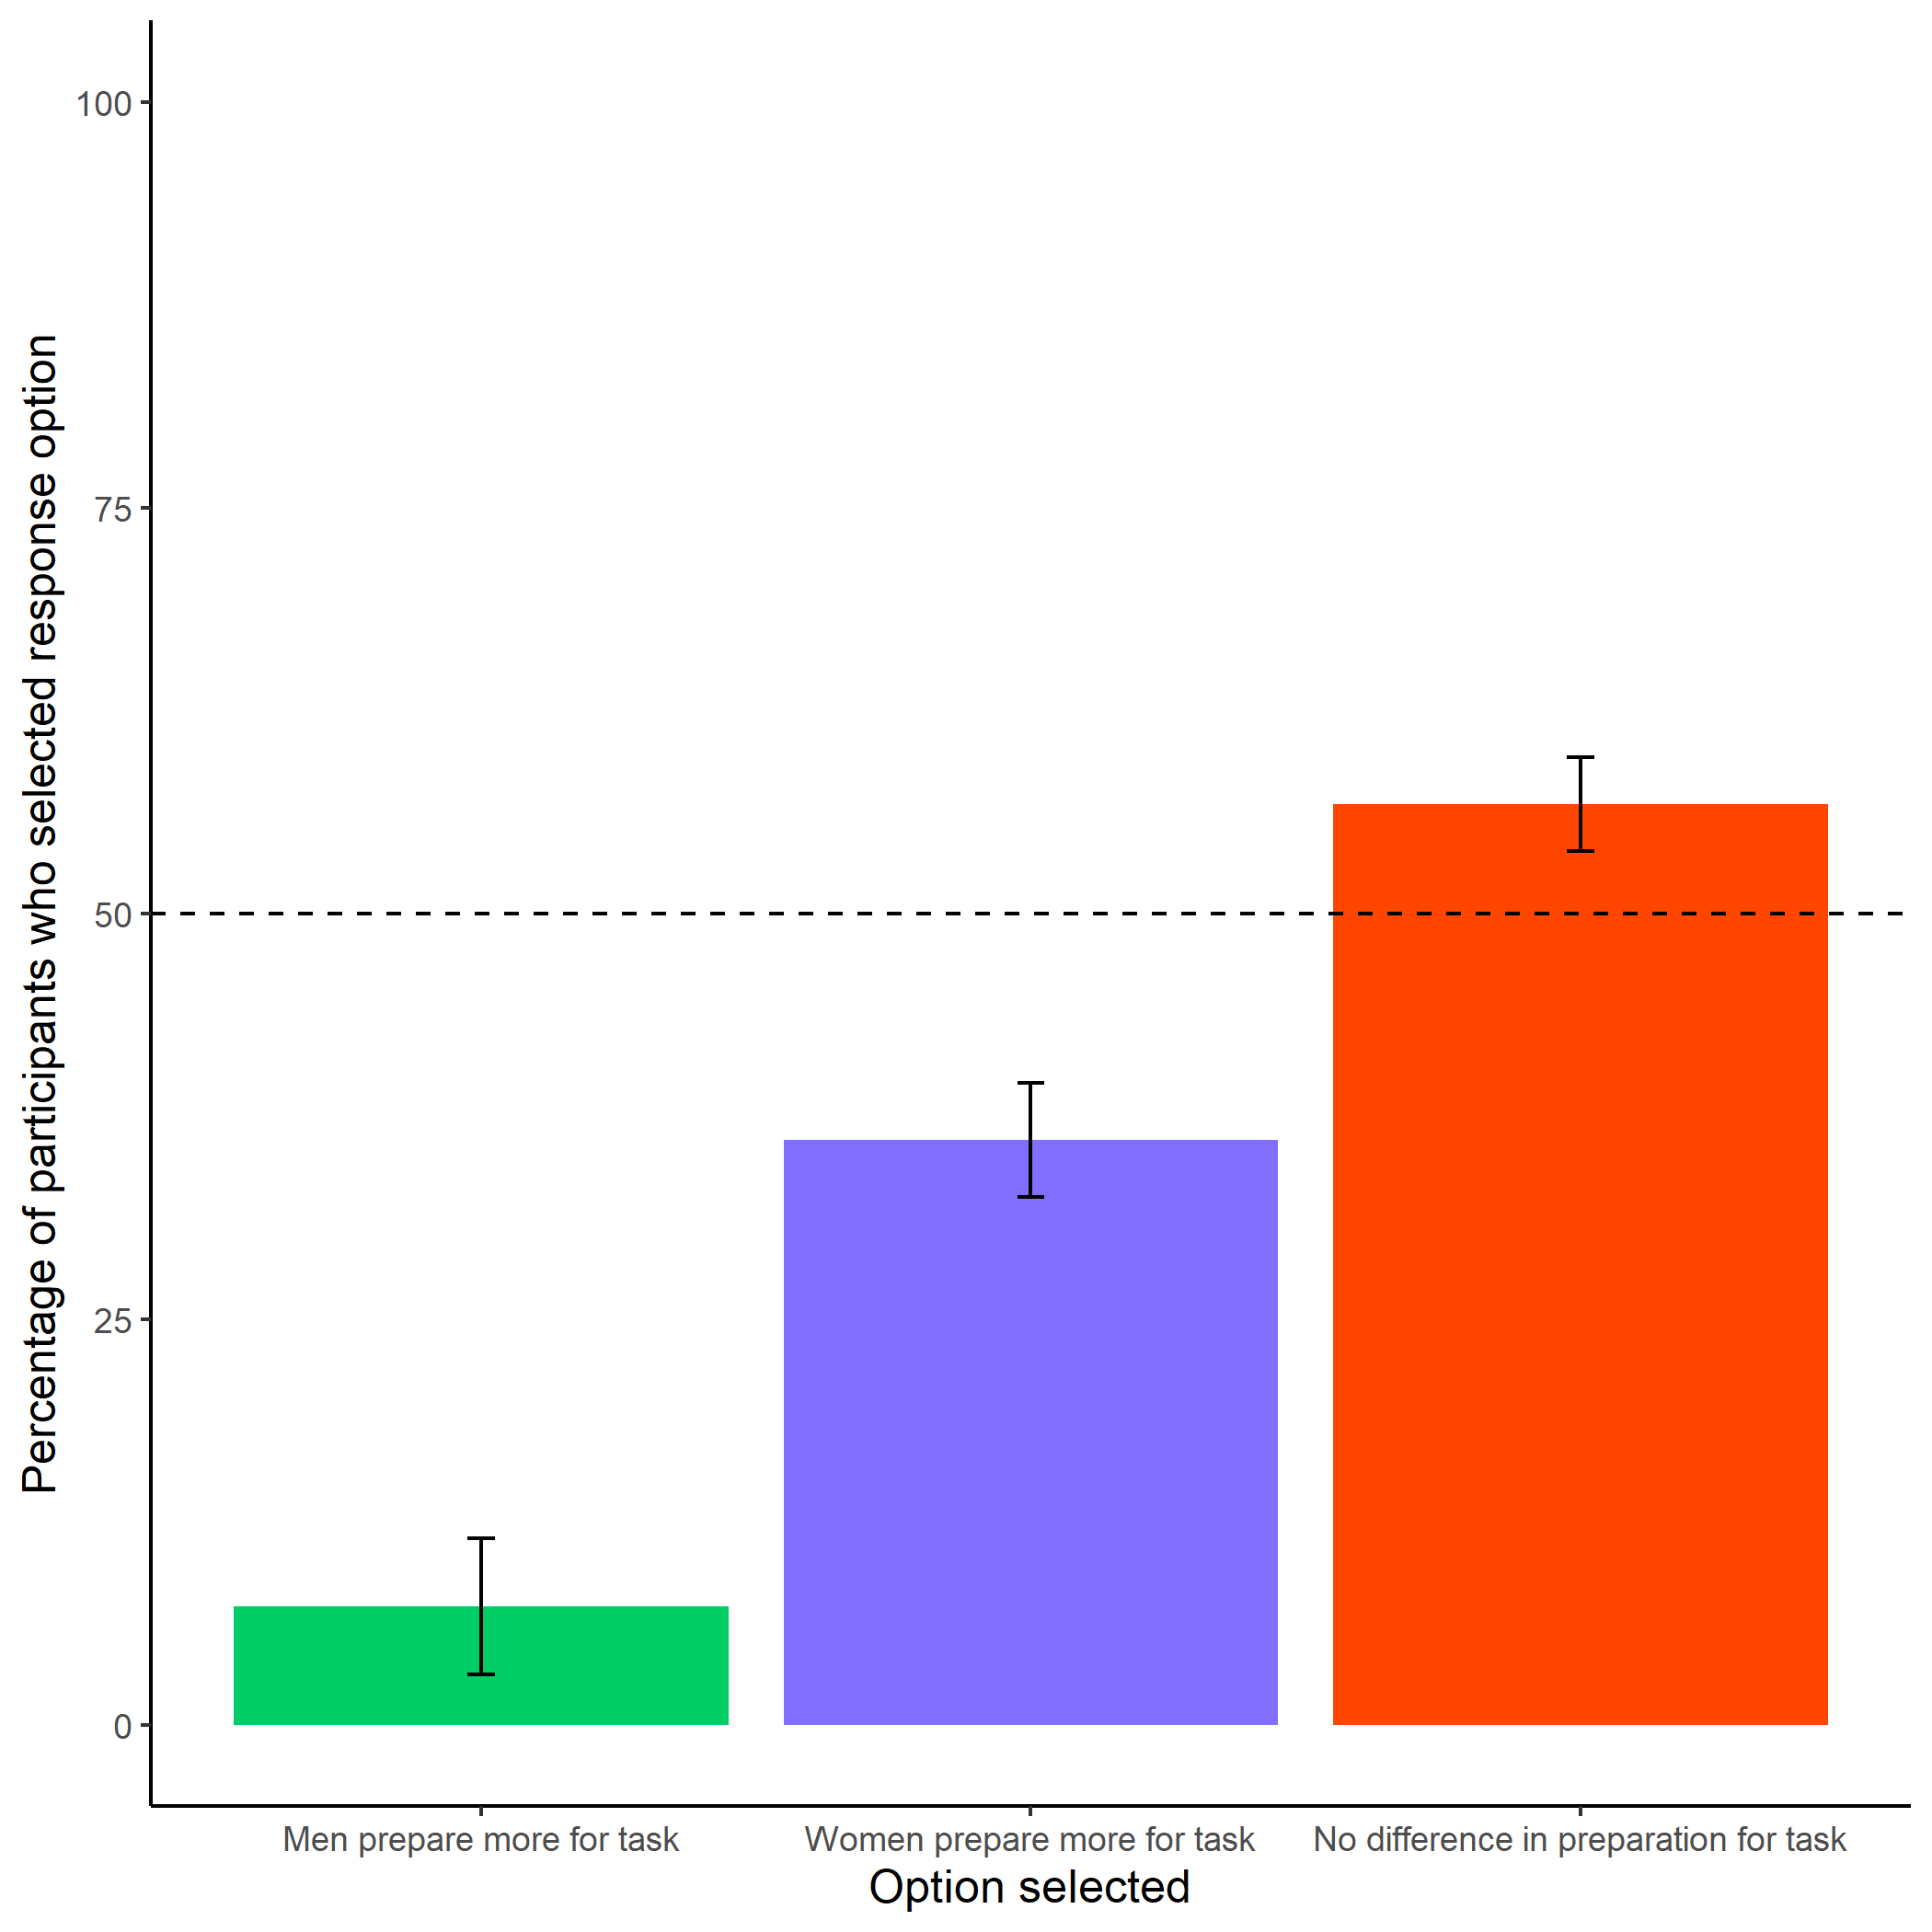
\includegraphics[width=300px]{C:/Users/keana/OneDrive - PennO365/Comp_transfer2018/Penn/practice_study/gender-practice/study4/figs/fig07_perc-task-gender-pract} 

}

\caption{Proportion of participants that predicted women would spend more time preparing for the multiplication task, men would spend more time preparing for the multiplication task, or that there would be no gender differences in preparation for the task. A significantly larger proportion of participants expected women to spend more time preparing for the multiplication task. Error bars represent standard errors.}\label{fig:s303}
\end{figure}

\begin{figure}

{\centering 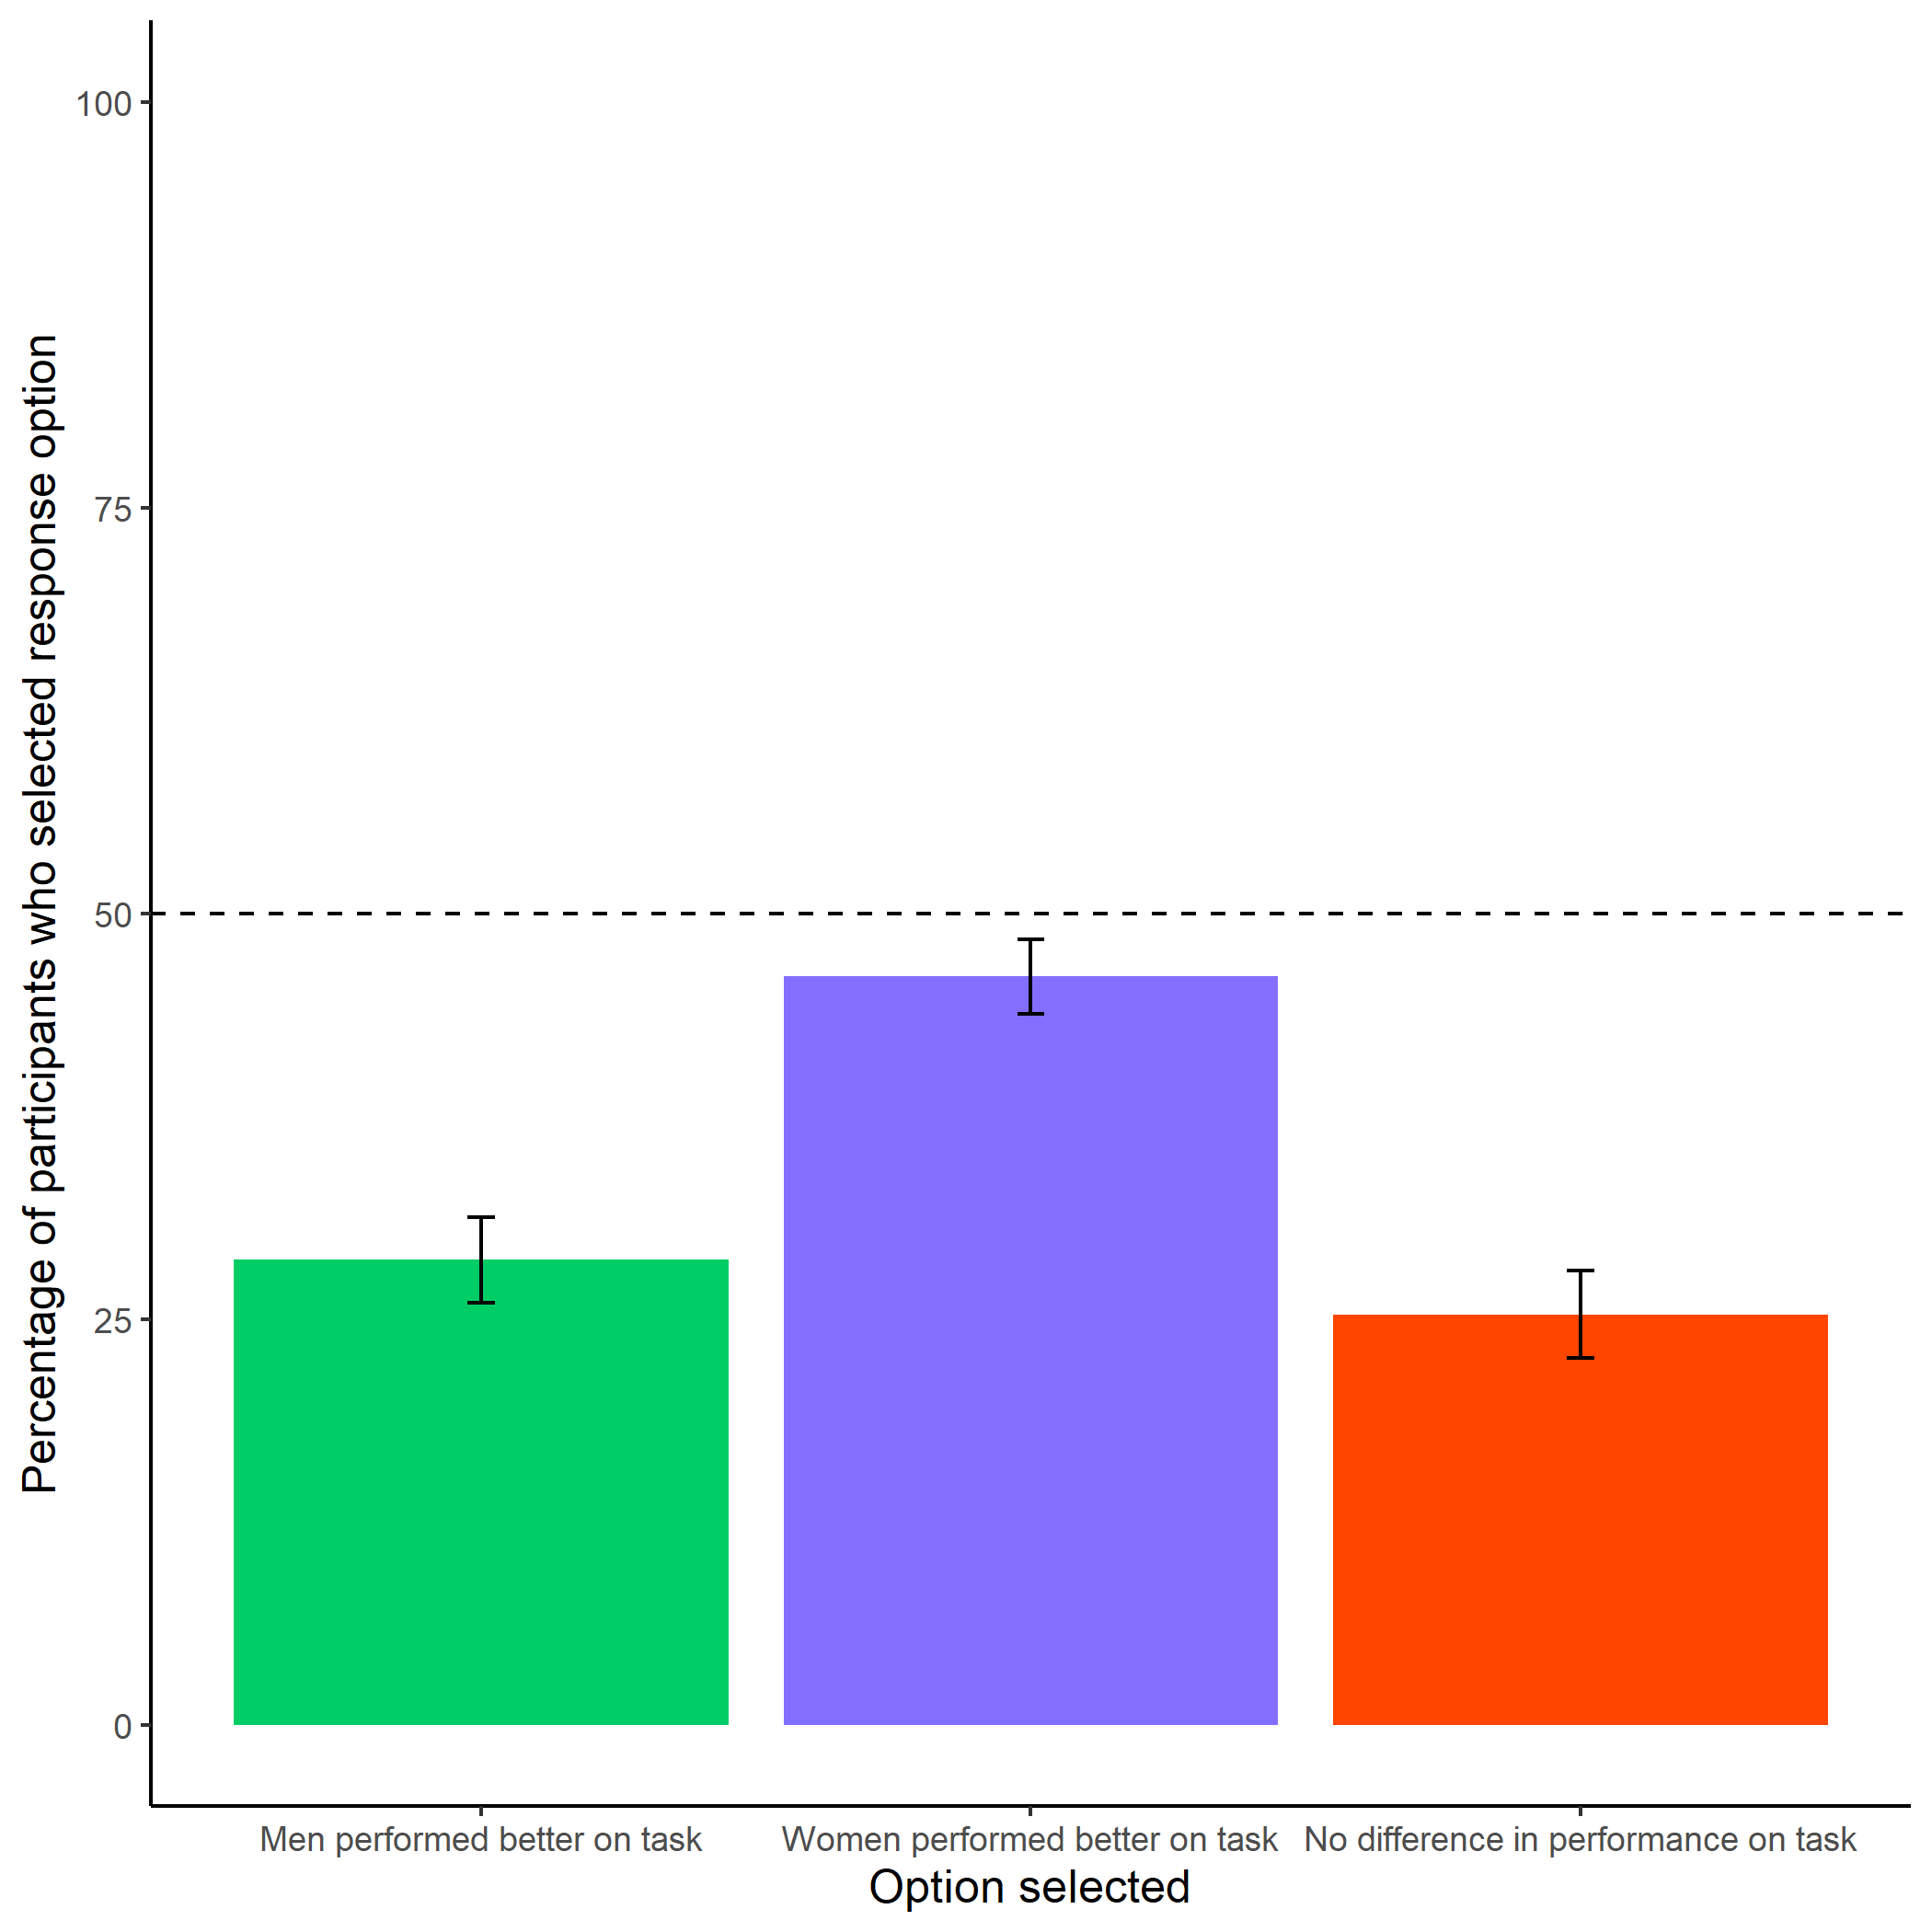
\includegraphics[width=300px]{C:/Users/keana/OneDrive - PennO365/Comp_transfer2018/Penn/practice_study/gender-practice/study4/figs/fig10_better-gender-guess} 

}

\caption{Proportion of participants that predicted women would correctly solve more problems on the multiplication task, men would correctly solve more problems on the multiplication task, or that there would be no gender difference in performance on the multiplication task. A significantly larger proportion of participants expected there to be no gender difference in performance on the multiplication task. Error bars represent standard errors.}\label{fig:s304}
\end{figure}

\begin{figure}

{\centering 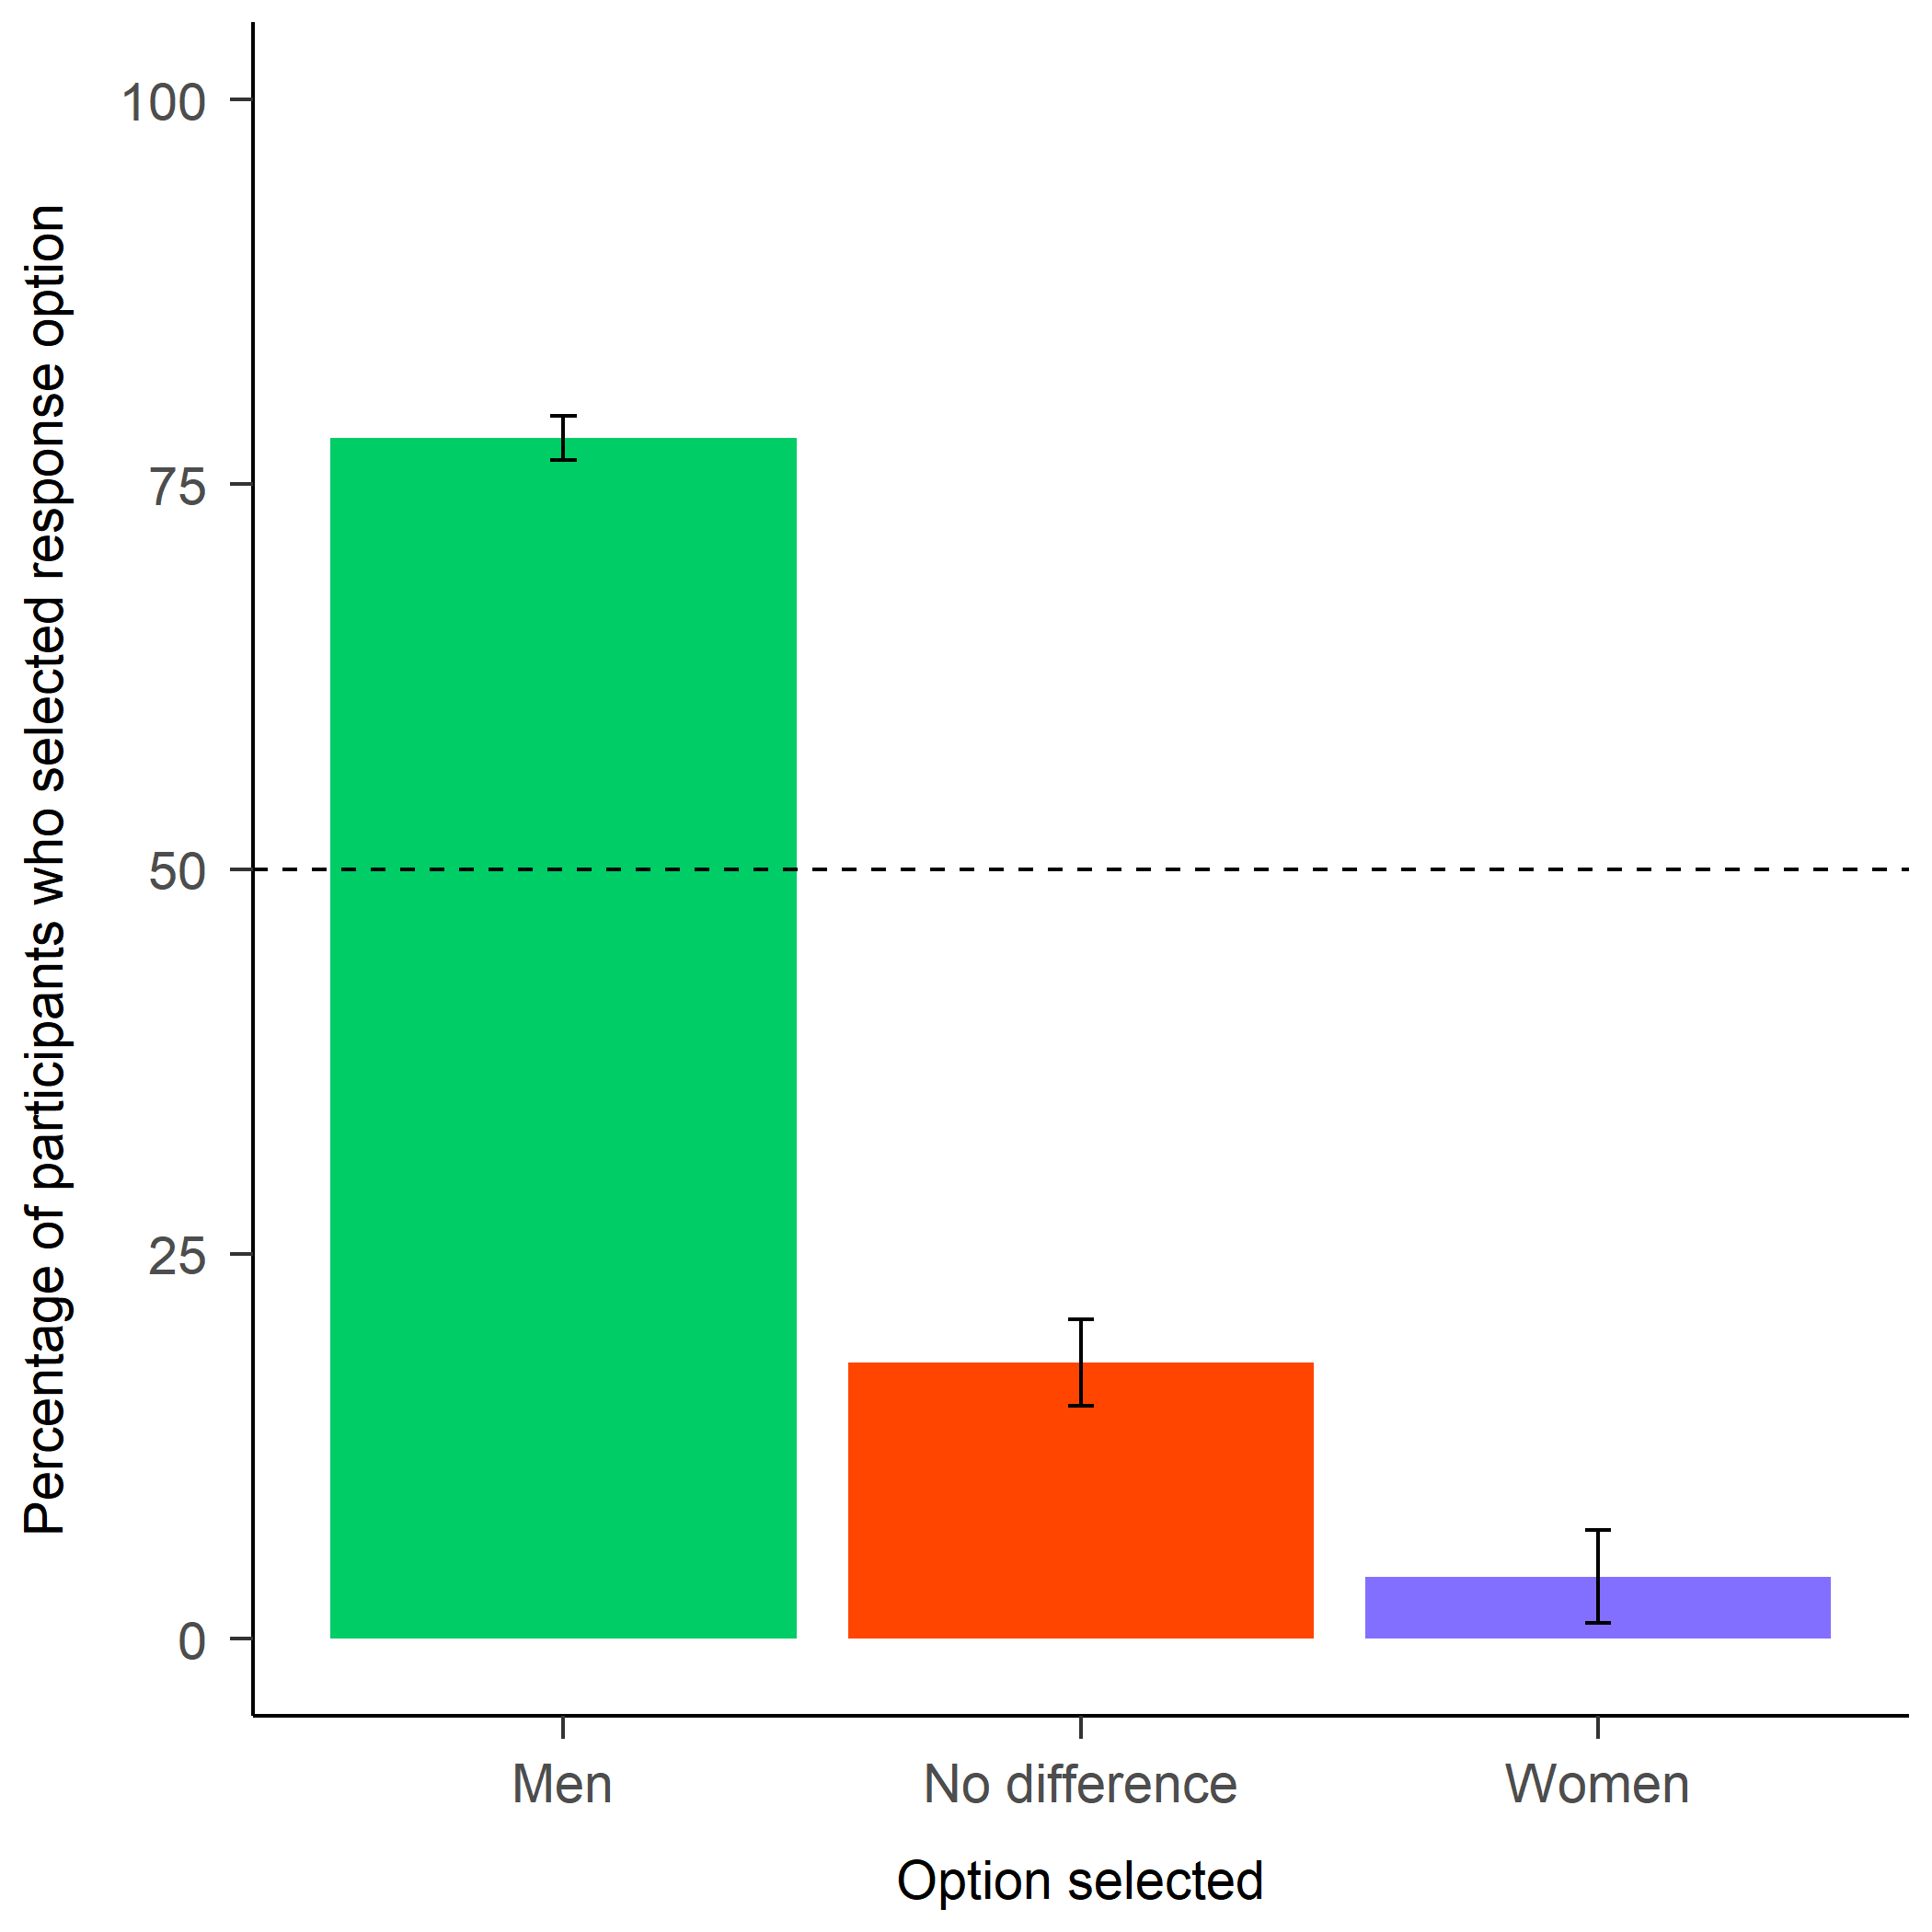
\includegraphics[width=300px]{C:/Users/keana/OneDrive - PennO365/Comp_transfer2018/Penn/practice_study/gender-practice/study4/figs/fig09_perc-gender-comp} 

}

\caption{Proportion of participants that predicted women would choose the tournament payment scheme more often, men would choose the tournament payment scheme more often, or there would be no gender differences in the choice to compete. A significantly larger proportion of participants expected men to be more likely to choose to compete. Error bars represent standard errors.}\label{fig:s305}
\end{figure}

\begin{figure}

{\centering 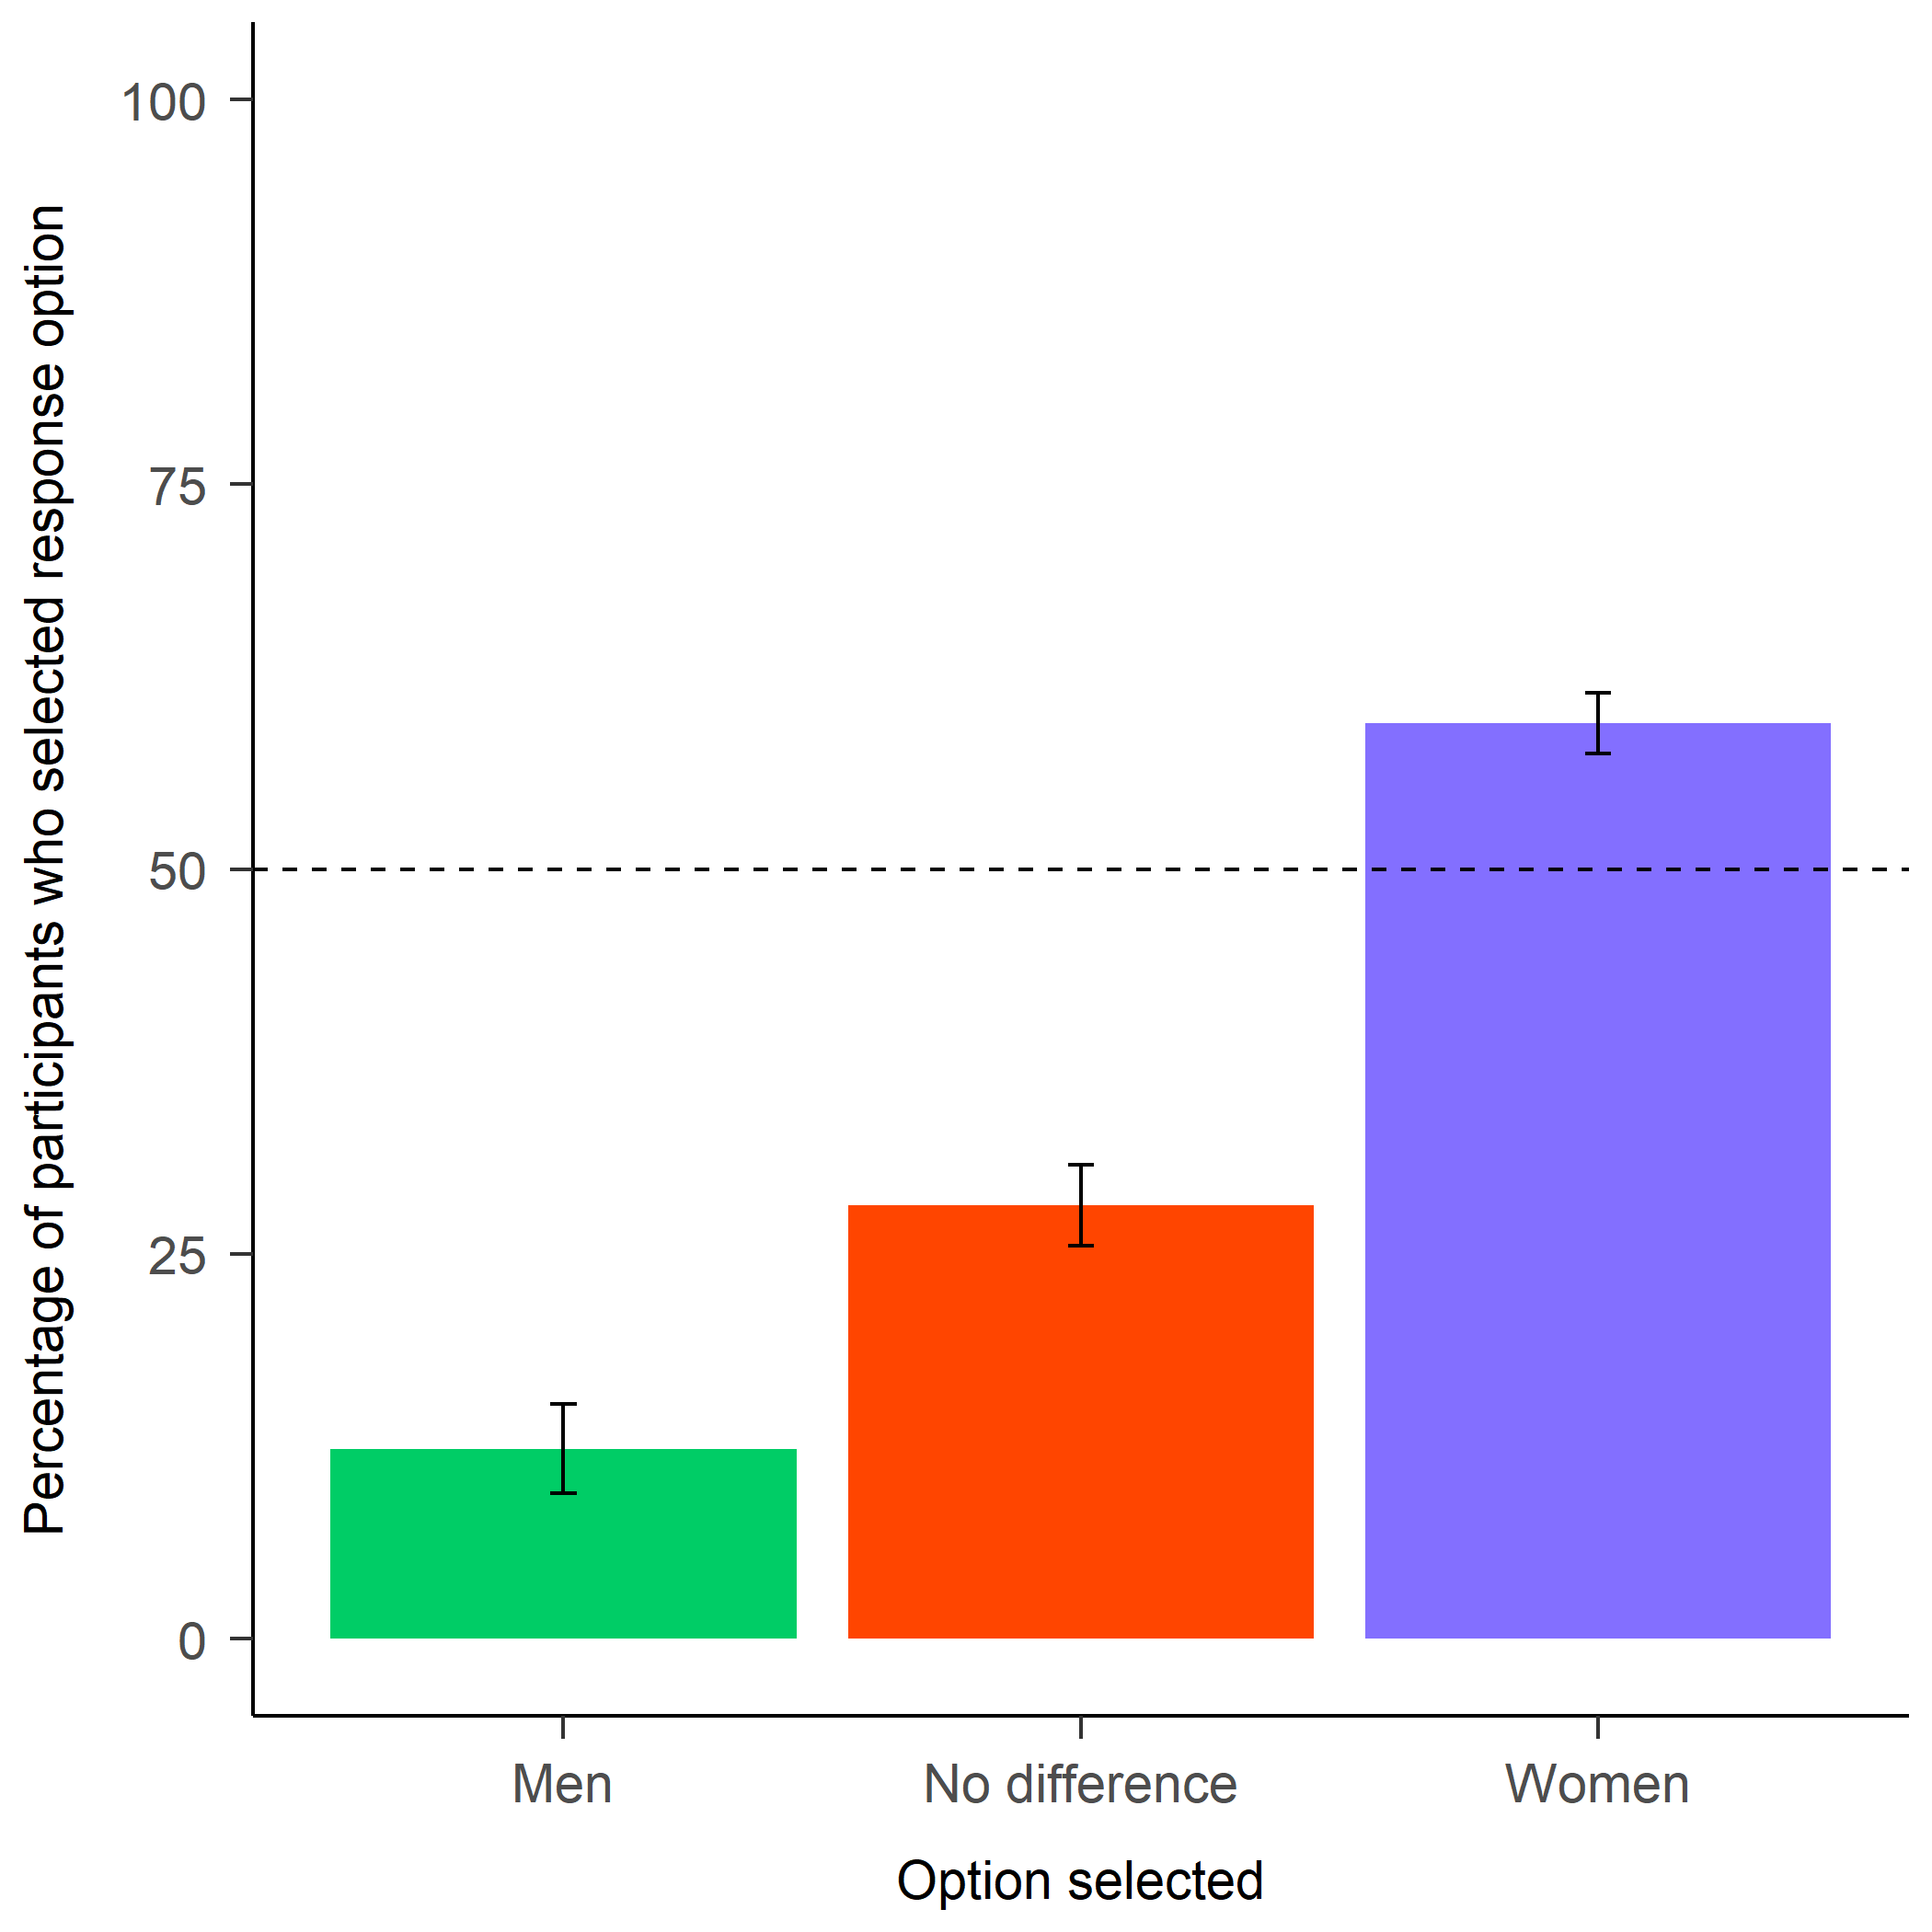
\includegraphics[width=300px]{C:/Users/keana/OneDrive - PennO365/Comp_transfer2018/Penn/practice_study/gender-practice/study4/figs/fig08_perc-gen-gender-pract} 

}

\caption{Proportion of participants that predicted women prepare more in general, men prepare more in general, or that there are no gender differences in preparation in general. A significantly larger proportion of participants expected women prepare more in general. Error bars represent standard errors.}\label{fig:s306}
\end{figure}

\hypertarget{effects-of-gender-and-perceptions-on-practicing-3}{%
\subsubsection{Effects of gender and perceptions on practicing}\label{effects-of-gender-and-perceptions-on-practicing-3}}

Like the previous two studies, we explored whether women who believed other women prepare more were especially likely to prepare. To that end, we ran the same logistic regression with the choice to practice as the dependent variable and gender, beliefs about gender differences in preparation on most tasks, and the interaction between those two variables as the predictors. Notably, the predictors representing participants' beliefs in these models had three possible values: women, men, and no difference. Like the previous studies, we focus on the interaction effect between gender and participants' selecting women as the gender that spends more time preparing while controlling for all other effects in the model. We do not replicate the interaction effect found in the previous studies, such that women who said women generally prepare more on most tasks were not significantly more likely to prepare, \(b = 0.42\), 95\% CI \([-0.91\), \(1.82]\), \(z = 0.60\), \(p = .545\) (see Figure \ref{fig:pract-choice-by-gender-and-perc-gen-prep-bar-study4}). We ran the same analysis with participants' beliefs about gender differences in preparation for the multiplication task, gender, and the interaction between the two as predictors instead, and replicate the interaction effect from the previous studies, \(b = 2.40\), 95\% CI \([0.95\), \(3.99]\), \(z = 3.13\), \(p = .002\). However, in this case, the interaction effect appears to be driven by men being especially likely to prepare when they think men spent more time preparing for the multiplication task (see Figure \ref{fig:pract-choice-by-gender-and-perc-task-prep-bar-study4}).

\begin{figure}

{\centering 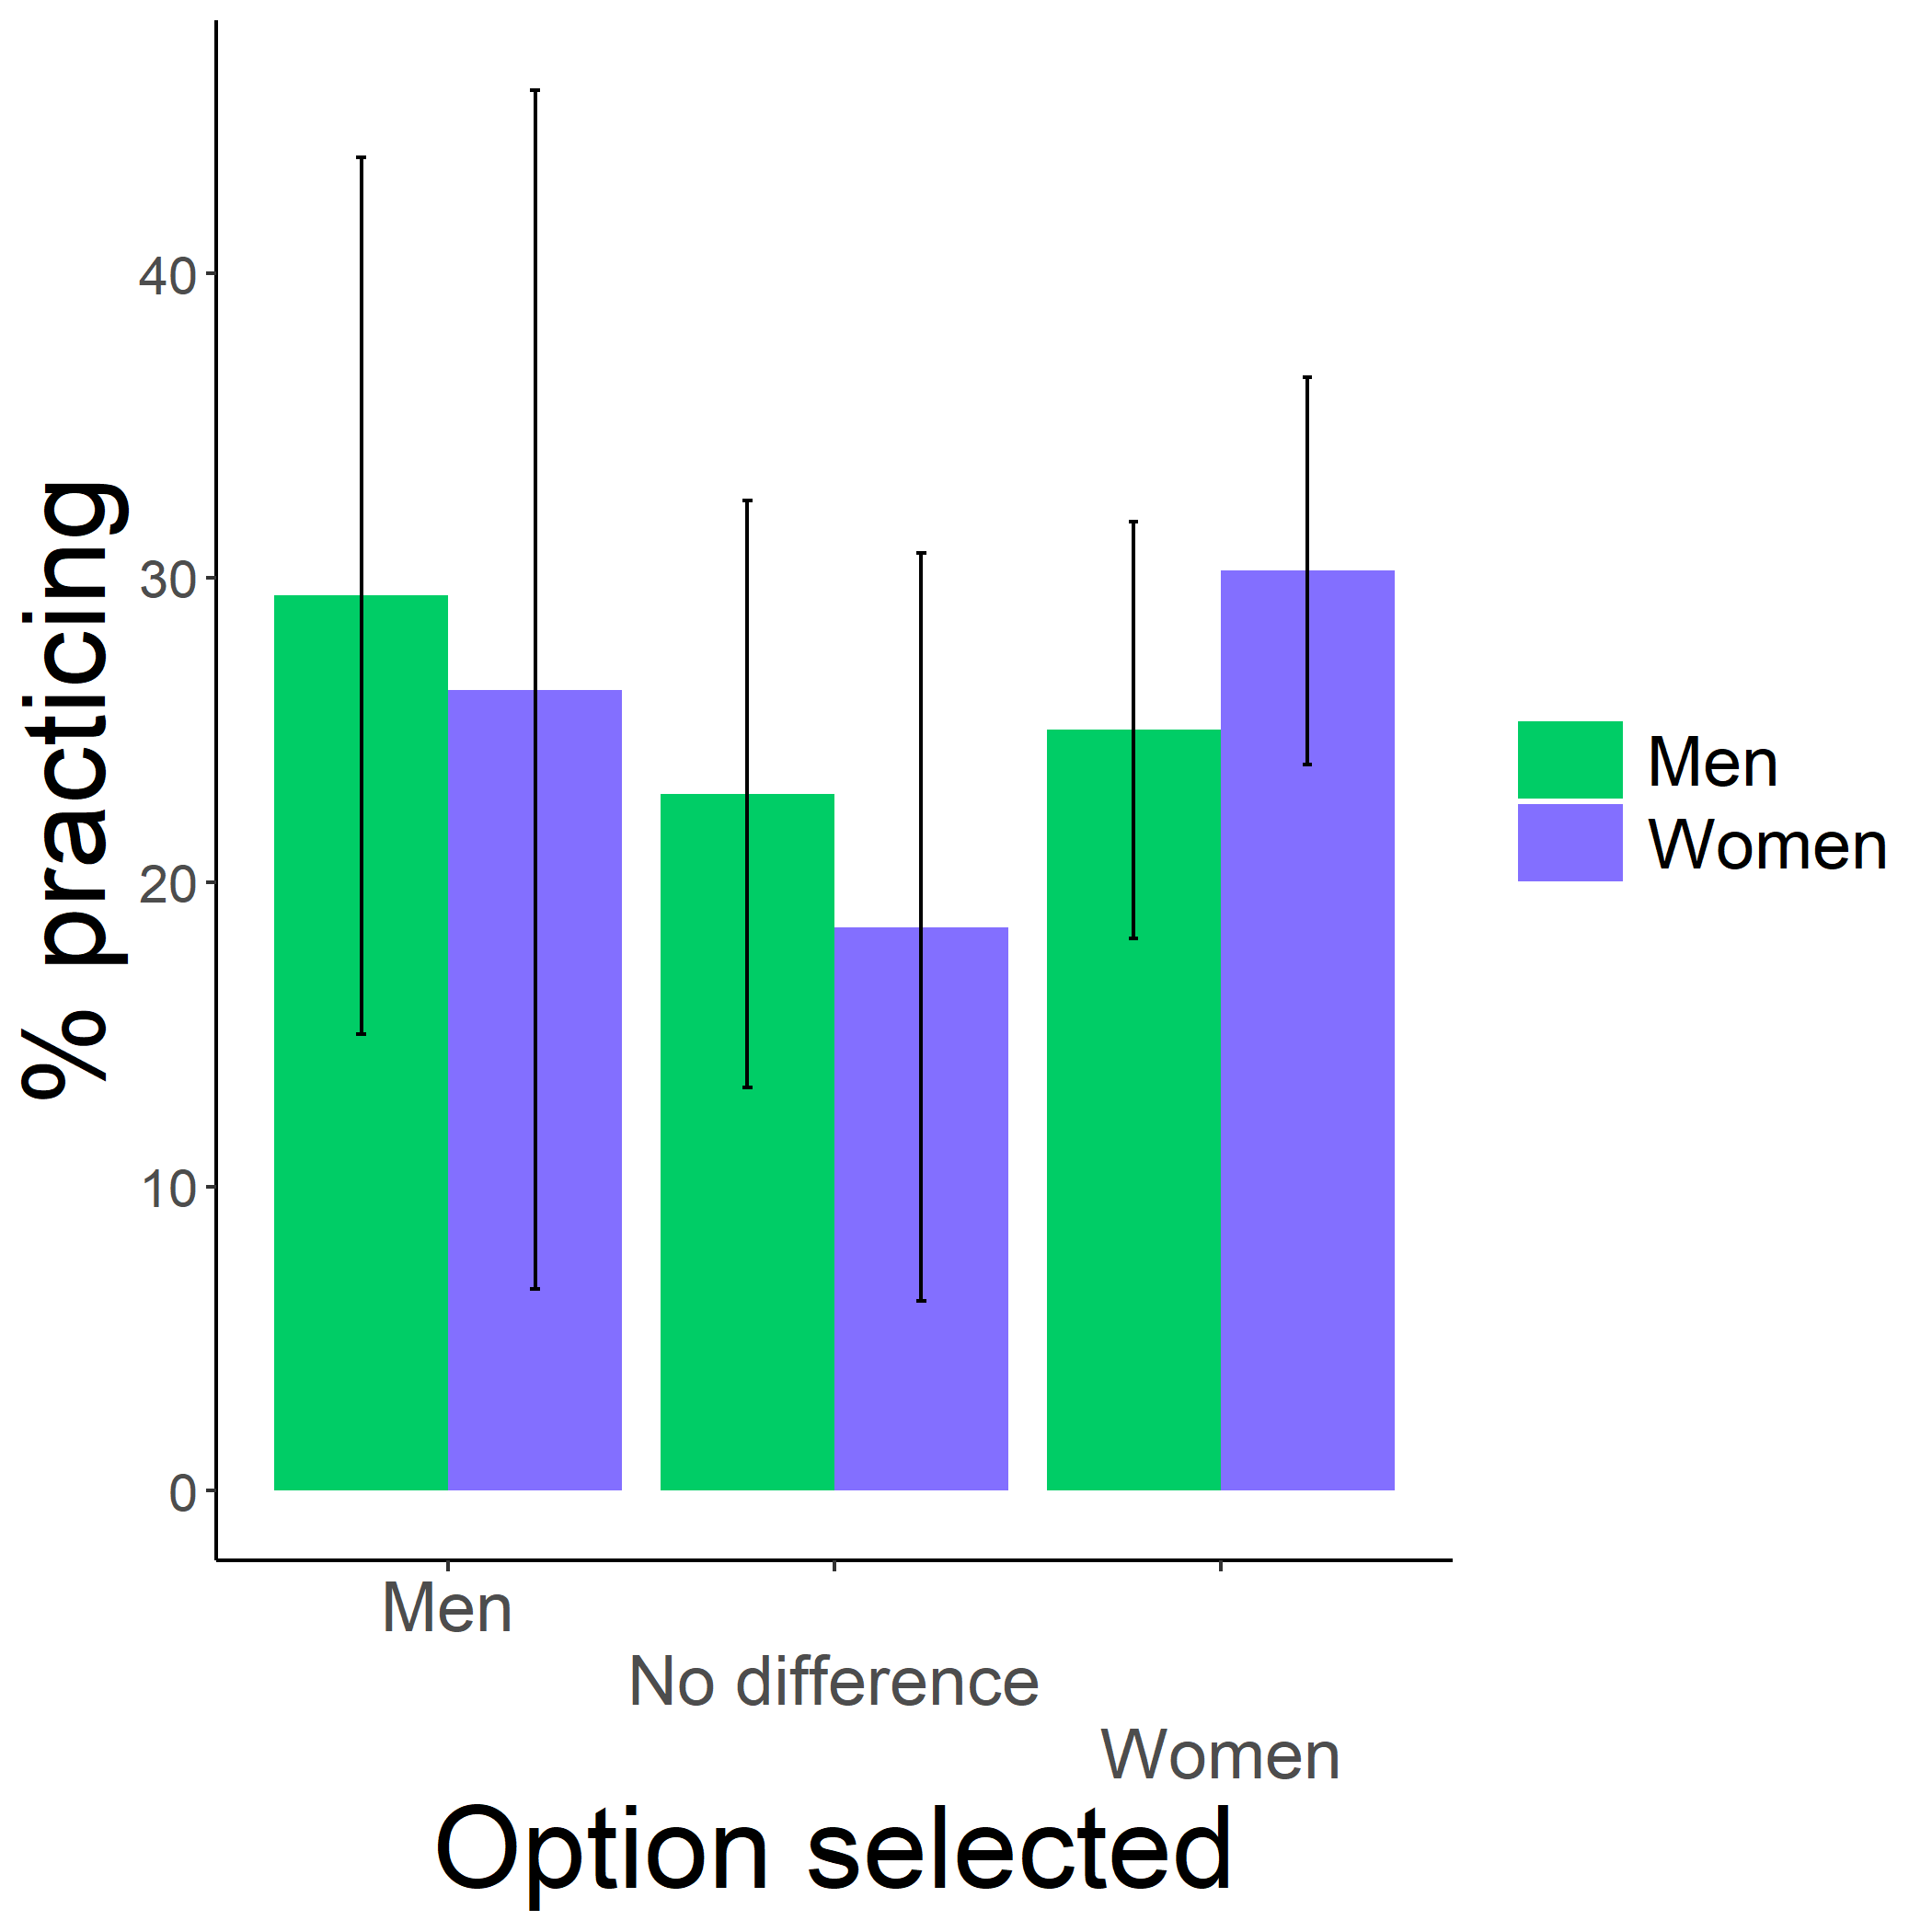
\includegraphics[width=300px]{C:/Users/keana/OneDrive - PennO365/Comp_transfer2018/Penn/practice_study/gender-practice/study4/figs/pract-choice-by-gender-and-perc-gen-prep-bar-study4} 

}

\caption{Proportion of men and women in Study 3 who chose to practice based on whether they thought men or women spend more time preparing on most tasks. In this study, participants also had the option to say there was no gender difference in preparation. It is worth noting that a small sample of participants (N = 136 participants chose to prepare across the entire study) are represented in this graph. Error bars represent standard errors.}\label{fig:pract-choice-by-gender-and-perc-gen-prep-bar-study4}
\end{figure}

\begin{figure}

{\centering 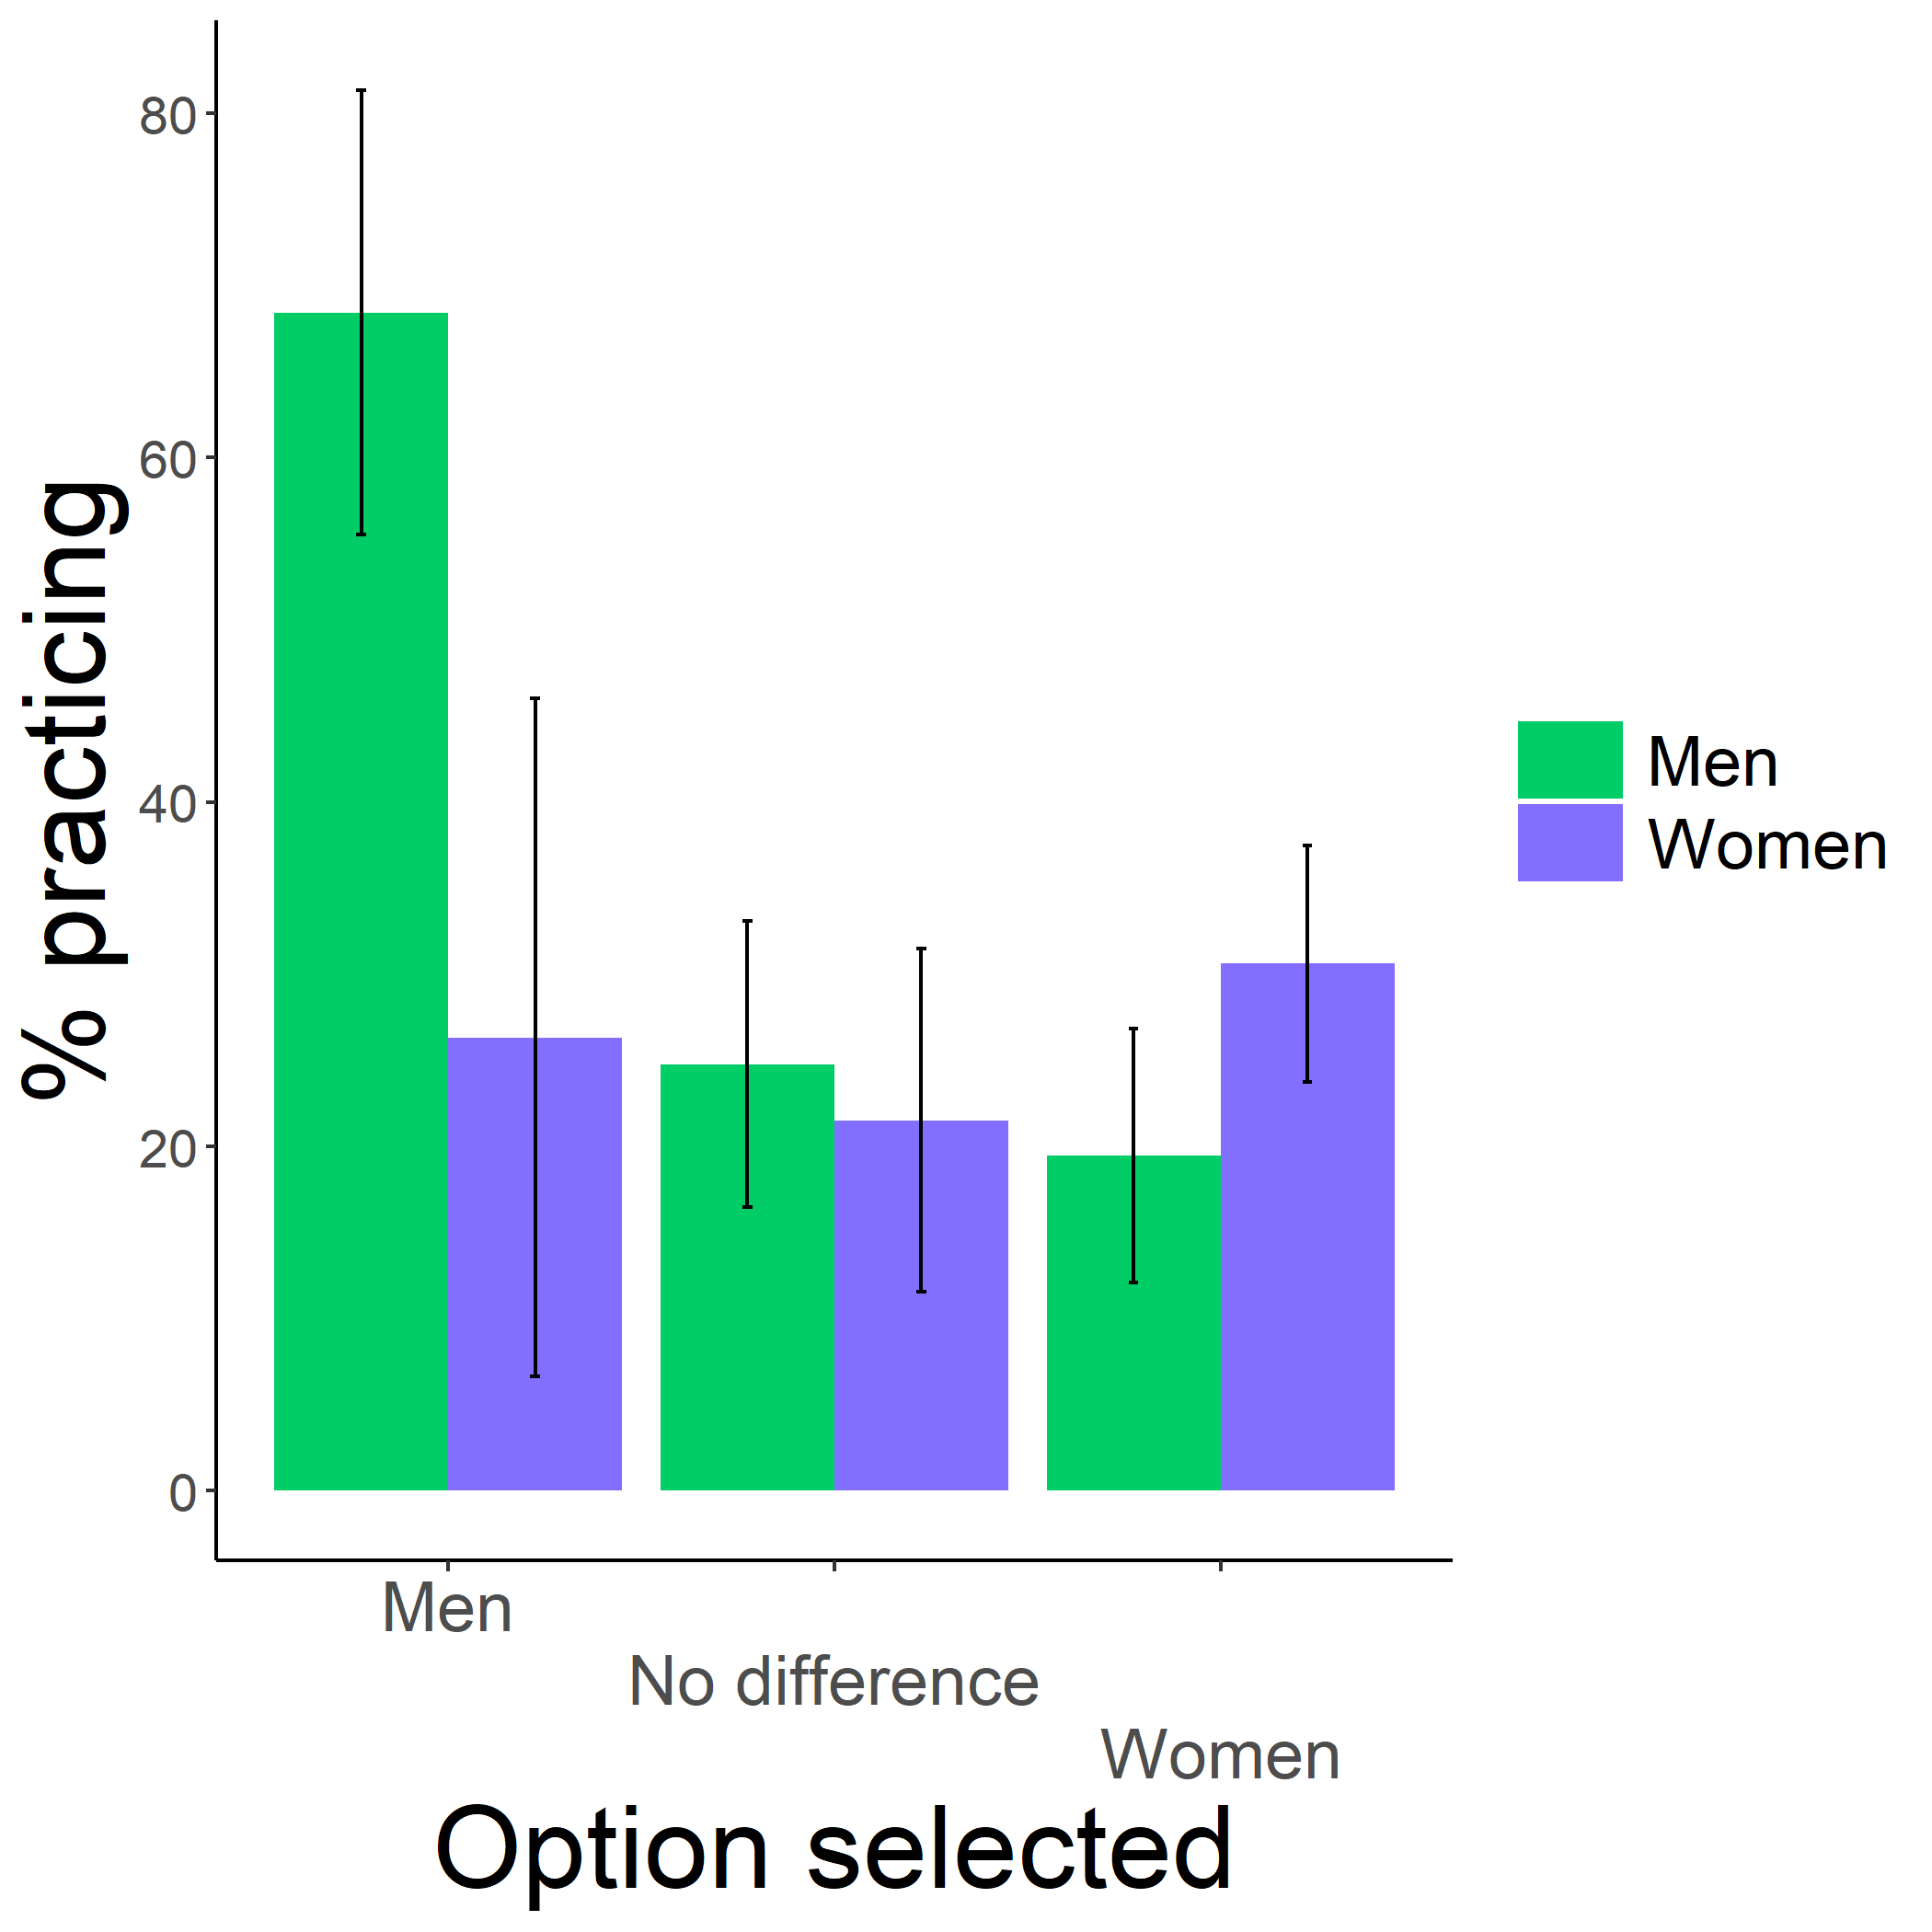
\includegraphics[width=300px]{C:/Users/keana/OneDrive - PennO365/Comp_transfer2018/Penn/practice_study/gender-practice/study4/figs/pract-choice-by-gender-and-perc-task-prep-bar-study4} 

}

\caption{Proportion of men and women in Study 3 who chose to practice based on whether they thought men or women spend more time preparing for the multiplication task. In this study, participants also had the option to say there was no gender difference in preparation. It is worth noting that a small sample of participants (N = 136 participants chose to prepare across the entire study) are represented in this graph. Error bars represent standard errors.}\label{fig:pract-choice-by-gender-and-perc-task-prep-bar-study4}
\end{figure}

\hypertarget{validating-the-perceived-utility-of-preparation-condition-over-control-condition}{%
\subsubsection{Validating the perceived utility of preparation condition over control condition}\label{validating-the-perceived-utility-of-preparation-condition-over-control-condition}}

Since we did not find any effect of the unlimited preparation condition, and this study uses a novel control task that has not been used in previous studies, we ran additional analyses to test whether participants actually felt like the preparation condition was more useful for performance on the paid multiplication task than the control condition. It is possible we did not observe an effect of condition on the choice to compete, nor an interaction effect between gender and condition, because participants simply did not think the preparation task would be more helpful for improving their performance relative to the control condition.

To explore this null effect further, we looked into how much participants were choosing to practice across conditions, which may provide insight into why there was no difference in the choice to compete across conditions. It is possible that participants in the control condition decided to complete subtraction problems at similar rates as participants in the preparation condition decided to complete multiplication problems, and if so, this may have led them to compete at similar rates because the subtraction tables felt easier than the multiplication tables, and therefore boosted their confidence or reduced perceptions of risk. Contrary to this possibility, we find that participants in the practice condition tended to choose to study, \(b = 0.69\), 95\% CI \([0.43\), \(0.95]\), \(z = 5.20\), \(p < .001\), and practice, \(b = 0.78\), 95\% CI \([0.47\), \(1.10]\), \(z = 4.89\), \(p < .001\), the multiplication tables at significantly higher rates relative to participants in the control condition where they completed subtraction problems.

In further evidence of the perceived utility of the preparation condition for improving performance on the paid multiplication task, participants across both conditions tended to believe when asked in the manipulation check that practicing multiplication problems would be more likely to improve performance on the paid multiplication task than practicing subtraction problems, \(\chi^2(1, n = 1072) = 548.50\), \(p < .001\).

\hypertarget{discussion-2}{%
\subsection{Discussion}\label{discussion-2}}

In this final test of the effects of the opportunity to prepare on the choice to compete, we explored whether having unlimited time to prepare would reduce the gender gap in competitiveness. First, we test whether there is a gender difference in competitiveness, which we do find again within the context of this design. That is, women do indeed compete less than men when gender is included as a predictor by itself in the model - but the fact that the effect disappears when controlling for risk attitudes, confidence, and task scores provides further evidence that competitiveness may not be a stand-alone trait. We also replicate the effects of gender on risk attitudes and confidence. In this study, we do not find evidence of a gender difference in task score when controlling for confidence and risk attitudes, like Study 2. Thus, Study 1 is the only study thus far in the dissertation that has found a gender difference in task scores that does not appear to be explained by gender differences in risk attitudes or confidence.

\hypertarget{summary-of-main-experimental-results-2}{%
\subsubsection{Summary of main experimental results}\label{summary-of-main-experimental-results-2}}

Next, we explored the main experimental results for the intervention attempting to reduce the gender difference. We hypothesized that being assigned to the unlimited preparation condition that closely resembled the paid task would lead participants to choose to compete more often than participants who completed the control subtraction task that was not relevant to the paid task. In support of this assumption, when asked which condition they thought would be most helpful for improving performance on the multiplication task during the manipulation check, participants resoundingly chose the preparation condition over the control condition. Participants' responses on the manipulation check aligned with their choices to prepare across conditions, such that participants in the unlimited preparation condition were significantly more likely to choose to study and practice relative to participants in the control condition. Overall, we have evidence that the subtraction task was an appropriate choice for the control condition, as participants thought that it would be less likely to help their performance on the paid task relative to the multiplication task. Despite both behavioral and self-report evidence that participants thought the unlimited preparation condition would be more helpful for performance, we did not find evidence that condition assignment affected participants' choices to compete. Yet again, contrary to our hypothesis of an interaction between gender and condition, the effect of the unlimited opportunity to prepare before completing the paid task did not differ by gender.

\hypertarget{gender-differences-in-preparation-4}{%
\subsubsection{Gender differences in preparation}\label{gender-differences-in-preparation-4}}

Like the previous studies, the gender difference in preparation was also an important part of our analyses. Yet, in this study we do not find evidence of a gender difference in the choice to prepare. There are a few possible reasons we did not replicate the effect of gender on the choice to prepare. The discrepancy could be explained by the lower number of participants in the preparation condition relative to previous studies given the random assignment to condition. For this reason, we may have had less power in estimating the effects of gender on the choice to prepare. It is also possible that differences in the design of this study relative to the previous two studies drove the differences, which will be further explored in the overall discussion section.

In this study, we changed the nature of preparation - such that we had the novel opportunity to explore different ways of measuring preparation, including the choice to study multiplication tables and the amount of time a participant spends studying multiplication tables. With these new measures, we find that, among participants who chose to study the tables, women spend more time on the page (presumably studying, although we cannot directly attest to that, given the online nature of the experiment), though they did not choose to study at significantly higher rates than men. Thus, we have mixed evidence based on these new measures that women prepare more than men.

\hypertarget{perceptions-of-gender-differences-in-preparation-performance-and-competitiveness-4}{%
\subsubsection{Perceptions of gender differences in preparation, performance, and competitiveness}\label{perceptions-of-gender-differences-in-preparation-performance-and-competitiveness-4}}

Like the previous two studies in this dissertation, we explored participants' perceptions of gender differences to see whether there tends to be consistency in beliefs about gender differences in performance on the multiplication task, along with gender differences in the choice to prepare and compete, and if so, whether these beliefs aligned with the actual results found. Importantly, participants were again incentivized to guess the study results correctly to reduce the likelihood that participants would respond in a socially desirable way.

Notably, we added a third response option to the measures in this study, such that participants could indicate that they did not expect a gender difference in a given behavior. The third response option served as a test of robustness, since one could argue that the two-response option measures used in previous studies force participants to choose between indicating men or women when they would have otherwise indicated there was no gender difference in a given behavior.

Yet, contrary to that argument, the results mirror results found in previous studies, suggesting that there are consistent beliefs about gender differences in competitiveness and preparation, despite the consistency in beliefs about a \emph{lack} of gender differences in performance.

Like the previous studies, we also explored whether these perceptions are aligned with individuals' practicing behavior. However, we do not find evidence that women's preparation behaviors were related to their beliefs about gender differences in preparation. It is entirely possible that the smaller proportion of participants that even had the opportunity to prepare in this study (per random assignment of preparation condition) did not provide sufficient power to test the interaction effect. In fact, out of the sample of participants in the preparation condition, only a total of 136 participants agreed to prepare, which may be too small of a sample to detect the interaction effect.

\hypertarget{summary-2}{%
\subsubsection{Summary}\label{summary-2}}

Overall, we find from Study 3 of Chapter 1 that our manipulation of the unlimited opportunity to prepare did not reduce the gender difference in competitiveness. Like Studies 1 and 2, we show that the gender difference in competitiveness itself is explained by gender differences in risk attitudes and confidence. However, we do not replicate the effect that women chose to prepare more than men. Even still, participants believed that women prepared more than men both in general and on the multiplication task, even after we added a third response option where participants could indicate there were no gender differences in preparation. We do not find evidence that women's preparation behaviors are related to their perceptions of gender differences in preparation, though we argue that we may have not had enough power for testing the interaction effect in the current study.

\hypertarget{chapter-3-effects-of-competition-on-gender-differences-in-the-choice-to-prepare}{%
\chapter{Chapter 3: Effects of competition on gender differences in the choice to prepare}\label{chapter-3-effects-of-competition-on-gender-differences-in-the-choice-to-prepare}}

\hypertarget{introduction-1}{%
\section{Introduction}\label{introduction-1}}

Competitions are increasingly prevalent in the global labor market \autocite{Lavy2004,Lemiuex2009} and the winners of competitions are disproportionately rewarded \autocite{Frank2010}. Much work on gender differences in competitiveness has focused on designing interventions that increase women's willingness to compete. We test the viability of one such intervention in Chapter 1 of this dissertation by providing men and women opportunities to practice before competing. While the intervention ultimately did not increase women's competitiveness, the studies in Chapter 1 revealed that women prepare more than men. Moreover, both men and women believed that women would be more likely to practice. Thus, a new gender difference in preparation was discovered. In the current Chapter, we ask whether competitions themselves disproportionately increase rates of practicing among women, such that women are especially likely to prepare before entering competitive environments relative to non-competitive environments. Additionally, we explore whether gender stereotypes may be driving the gender difference to practice. While considerable efforts have been made to understand why men are more likely than women to choose to compete, less attention has been paid to whether and how men and women may differentially respond to competitions. Yet, understanding downstream consequences of nudging or forcing women into competitions may too help address gender disparities in economic outcomes \autocite{Blau2017,Altonji1999}.

\hypertarget{the-gender-gap-in-labor-market-outcomes-and-preferences-for-competition}{%
\subsection{The gender gap in labor market outcomes and preferences for competition}\label{the-gender-gap-in-labor-market-outcomes-and-preferences-for-competition}}

Compensation packages based on performance pay, such as bonuses, commissions, and piece-rate payments, have risen in popularity relative to hourly/salaried pay, especially among workers in the highest tiers of occupations \autocite{Hall1998,Murphy1999,Cunat2005,Lemiuex2009}. There is evidence that the increasing use of performance pay lends itself to wage inequality. \textcite{Lemiuex2009} showed that an increased dependence on performance pay during the late 1970's and early 1990's accounted for 21\% of the observed growth in variance of men's wages. Bonuses and commissions, arguably the most competitive compensation schemes, may be especially important in driving the large disparity between the highest and lowest percentile earners within organizations \autocite{Bell2010,Bell2014,Benabou2016}. Importantly, performance pay may contribute to the gender wage gap too. Using data from the National Longitudinal Surveys of Youth, \textcite{McGee2015} show that women are less likely to be employed in occupations that receive bonuses, and simultaneously are more likely to receive piece-rate pay -- the least competitive of all forms of performance pay, where workers are paid based on their absolute output.

The gender wage gap refers to the difference in earnings between men and women, with men earning more, on average, than women worldwide. While the gender gap has decreased over the last three decades, the improvements have been modest. For instance, it is estimated that the ratio of women's to men's wages in the United States increased to only 67\% in 2016 from 53\% in 1986 \autocite{Gharehgozli2020}. While numerous factors have been implicated in contributing to the gap, including human capital variables (e.g., gender gaps in education and work experience) \autocite{Goldin2006a}, workforce interruptions and fewer hours among women \autocite{Blau2017a}, persistent gender segregation by field and occupation \autocite{Blau2017,Goldin2014}, along with discrimination \autocite{Blau2017}, some researchers have looked to gender differences in men's and women's willingness to compete and to a lesser extent, behavior that results when required to enter a competition. An expanding literature in both psychology and experimental economics suggests that men, compared to women, are more willing to enter competitions. This finding was first documented in a foundational experiment by \textcite{Niederle2007}, and has since been replicated numerous times across populations \autocites[for reviews, see][]{Croson2009,Niederle2011,Niederle2017a}[and][]{Shurchkov2018}, including among hunter-gatherers \autocite{Apicella2015}.

Typically, researchers measure competitiveness as one's willingness to enter a tournament where success and thus, earnings, depend on outperforming (an)other player(s). Participants who prefer tournament payment schemes over piece-rate payment schemes, where payments are solely determined by the number of successfully completed units, are said to be competitive \autocite{Niederle2007}. Importantly, this laboratory measure of competitiveness predicts education and career choices, along with earnings outside the lab \autocite{Buser2014,Zhang2012,Buser2017c,Samek2019,Berge2015,Reuben2015,Reuben2017,Buser2017b,Buser2020a}, and thus may help explain gender gap in labor market outcomes.

To date, most of the research on gender differences in competitiveness has focused on i) either explaining the sources of the gender difference -- for instance, men tend to be more confident and risk-seeking than women \autocite[e.g.,][]{Veldhuizen2017} or ii) designing interventions to encourage women to compete more \autocite{Balafoutas2012,Sutter2016,Cassar2016,Brandts2015,Niederle2013,Brandts2015,Healy2011,Alan2018}. For instance, \textcite{Kessel2021} find that telling participants about the gender difference in willingness to compete as well as the implications on earnings, reduces the gender gap in competitiveness. Crucially, less consideration has been paid to how competitions may differentially, and perhaps negatively, impact women in other ways, such as lowered performance both during and after competition, reduced desire to enter future competitions, or potential opportunity costs related to time spent (over) preparing when required to compete.

The rest of this introduction briefly summarizes the literature on how men and women may differentially respond to competitions at three specific time points (i.e., before, during, and after competition) and highlights the need for more work on how men and women may behave differently \emph{before} entering competitions. Second, we introduce several reasons for why preparation might be one specific behavior where gender differences before competition arise, with the expectation that women practice more than men, especially when competing. Finally, we introduce the current investigation, which experimentally tests whether and how competitions affect gender differences in preparation.

\hypertarget{gender-differences-in-response-to-competitive-environments}{%
\subsection{Gender differences in response to competitive environments}\label{gender-differences-in-response-to-competitive-environments}}

There are three major time points at which competition may affect men and women differently: before, during, and after competition. The majority of previous studies in this space have examined gender differences in response to competition during and after performance.

\hypertarget{during-competition}{%
\subsubsection{During competition}\label{during-competition}}

Many lines of work have explored the possibility of gender differences in performance under competitive pressure. Here, we summarize the work on different forms of competitive pressure, including studies that explicitly labeling one environment as competitive or, in other cases, impose certain rules or create performance contexts under which, although not explicitly labeled as competitive, reduce an individual's probability of earning a specific reward or reduce the amount of the reward they can earn, and as such, impose competitive pressure.

Although competitions are generally motivating and designed to improve performance by increasing effort \autocite{Connelly2014a,Murayama2012,Miller2019a}, previous research suggests that men perform better under competitive payment schemes relative to non-competitive payment schemes, while women's performance does not respond to competitions \autocite{Gneezy2003,Gneezy2004,Gunther2010,Samak2013,Booth2022,Gneezy2004,Niederle2011,Cotton2013}.\footnote{Though see \textcite{Dreber2011} for an exception} \textcite{Gneezy2003} show that there is no gender difference in performance when participants are solving mazes following a piece-rate payment scheme, but a significant gender difference in performance arises under a tournament payment scheme, with men performing better. \textcite{Gunther2010} replicate the effect of competition on gender differences in performance for a male-typed task, but find no gender differences in performance during competition for female-typed or gender-neutral tasks.

\textcite{Shurchkov2012} finds evidence that two types of pressure may explain part of the gender difference in competitiveness: task stereotypes and time constraints. Specifically, they find that women's performance suffers when they compete against others on a male-typed math task with high time pressure (2 minutes to perform), while there are no significant gender differences in performance during competition on a female-typed verbal task with low time pressure (10 minutes to perform). Also, they find that women are significantly more likely to choose to compete when there is low time pressure in a math tournament, while men's competition entry does not significantly vary based on the time pressure treatment.

There is also field evidence of gender differences in performance during competition. \textcite{Paserman2007} shows that women's probability of committing costly errors over the course of a tennis match increases at high-pressure moments, while men's probability of committing such errors does not significantly change across the match.

There is also extensive work on gender differences in performance and effort under competitive pressure within academic contexts \autocites{Iriberri2019,Cai2019,Ors2013,Azmat2016,Price2008}[see][ for a review on gender differences in math tests scores]{Niederle2010c}. For instance, in a study of gender differences in responses to different levels of competitive pressure on a Korean quiz show for student scholarships, researchers find that when stress is kept to a minimum, there are no gender differences in performance, but when certain knock-out rules are applied, a difference emerges \autocite{Booth2021}. \textcite{Morin2015} shows that the effect of an education reform that led to a double-cohort, and as such, increased competition for admission at the University of Toronto, increased men's average grades and the proportion of men who graduated on time relative to women, driven largely by men increasing their effort after the reform.

In a study examining performance during the GRE examination, \textcite{Attali2012} show that the gender gap in performance is significantly greater under the real GRE, which they demonstrated was driven by men increasing their effort, while women's effort stayed the same. The real GRE is inherently more competitive and higher-stakes than a voluntary experimental section of the GRE, providing further support for gender differences in performance in response to competitive pressure in the field.

There is also a growing literature showing that women are less willing to guess on exams \autocite{Pekkarinen2015,Baldiga2014,Iriberri2021}, which in turn negatively impacts their performance on said exams, widening the gender gap in performance under competitive pressure. \textcite{Riener2018} shows this phenomenon starts at an early age, with girls as young as eight years of age being significantly less willing to guess on exams relative to men.

\hypertarget{after-competition}{%
\subsubsection{After competition}\label{after-competition}}

During repeated competition, women tend to perform worse in subsequent performance rounds after losing, even if the monetary prize they lost was relatively meager, while men only perform worse in subsequent rounds if they lost the chance to win a large monetary prize \autocite{Gill2014}. Other research suggests women stop competing altogether after losing if given the choice. \textcite{Buser2019}, who examine the effects of losing while competing in the Dutch Math Olympiad on the choice to compete in subsequent years, show that men are just as likely to compete even if they lost the previous year, while women are less likely to compete again if they lost before. In a separate study, \textcite{Buser2016} shows that men react to losing during a competition by picking a more challenging target for their subsequent performance while women lower their performance.

Similarly, \textcite{Shastry2021} performed an experiment among Economics professors where they received feedback in the form of a letter from the editor on a hypothetical journal submission, with randomized decision outcomes (i.e., revise and resubmit, reject and resubmit, reject). They find that among the assistant professors within the sample, a flat rejection during the review process reduced women's beliefs in their probability of success in the future significantly more than men's - as quantified by their rating of the probability of publishing the paper in the same journal or in any leading journal. This gender gap in confidence does not hold among associate or full professors, which they argue is likely driven by survivorship bias.

In another study of the effects of feedback on subsequent gender differences in behavior and beliefs, \textcite{Coffman2021} examine both the role of task stereotypes (through a female-typed verbal quiz and a male-typed math quiz) and feedback (positive or negative) on both confidence and choice in a compensation scheme (piece-rate or tournament payment). They find that women's beliefs and choices after negative feedback are updated more negatively than men, regardless of their performance or choices before feedback. Overall, the current body of literature suggests that competitions may differentially impact women and men, both during and after said competitions.

\hypertarget{before-competition}{%
\subsubsection{Before competition}\label{before-competition}}

As mentioned previously, little research has examined how competitions may affect gender differences in behavior during another critical period: before an individual enters a competition, when they have the most control of their subsequent performance in the competition. Given previous research suggesting that women and men may respond differently during and after competitions, we expect that they will also employ different behaviors and have different perceptions of themselves and others in advance of a competition.

Our research in Chapter 1 suggests that women, compared to men, are more likely to prepare when given the opportunity. While the primary goal of this research was to experimentally test how preparation might influence gender differences in willingness to compete, a significant gender difference in the choice to practice emerged.\footnote{Note: The result was significant in only two of the three experiments conducted. In the experiment where the result was not significant, women still practiced at a higher rate than men.} Notably, the gender difference was present regardless of the payment option scheme chosen (i.e., the competitive tournament payment scheme or non-competitive piece-rate payment scheme), though such interaction effects may have been difficult to detect with the sample sizes employed. Moreover, because payment schemes were not randomized there may have been selection effects such that those who were more likely to compete may have also been less likely to prepare. Thus, whether tournament (relative to piece-rate) payment schemes lead women to prepare disproportionately more than men is still unknown.

\hypertarget{does-competition-elicit-a-gender-difference-in-preparation}{%
\subsection{Does competition elicit a gender difference in preparation?}\label{does-competition-elicit-a-gender-difference-in-preparation}}

There are three non-mutually exclusive reasons to suspect that competition would be especially likely to increase women's preparation before performance: the effects of competition on confidence, risk, and/or the stereotype that women prepare more than men.

\hypertarget{confidence-risk-and-rates-of-practicing}{%
\subsubsection{Confidence, risk, and rates of practicing}\label{confidence-risk-and-rates-of-practicing}}

Women may spend more time preparing than men, especially before competitions, in part because they are, on average, less risk-seeking \autocite{Croson2009,Dohmen2011b,Eckel2008,Bertrand2010a,Shurchkov2018} and confident \autocite{Bertrand2010,Lundeberg1994,Mobius2011,Barber2001,Croson2009,Shurchkov2018} than men.\footnote{See \textcite{Bandiera2022} for an exception} Indeed, both confidence and risk attitude have been implicated in driving the gender gap in willingness to compete \autocite{Veldhuizen2017,Gillen2019,Niederle2011}. The extent to which confidence and risk attitude account for the gender gap in willingness to compete is debated; some research suggests that competitiveness may be entirely explained by confidence and risk \autocite{Veldhuizen2017,Gillen2019} while other research suggests that there remains a residual gap in the choice to compete \autocite{Niederle2007}. Regardless of whether competitiveness is a stand-alone trait, confidence and risk attitude may lead to differences in how men and women react to competitions, possibly including the decision to prepare before competitions.

Preparing for a competition, through either practicing or studying, may be a strategy individuals employ before entering a competition. Since competitions, by definition, compare the performance among two or more individuals, they naturally lead to self-evaluation and comparative judgments of self with others - processes that are intimately linked to confidence. Thus, less confident individuals may prepare more in order to reduce the negative feelings caused by low confidence independent of any ambitions to win, since mastery is an important driver of confidence \autocite{Gist1992,Usher2008}. Given the aforementioned evidence that women tend to be less (over)confident than men \autocite{Mobius2011,Niederle2011,Croson2009,Lundeberg1994,Niederle2007,Bertrand2010a,Beyer1990,Beyer1997}, we may expect to see women preparing more than men, particularly in competitive contexts, which, again, naturally invoke self-other assessments.

Importantly, on top of their possible effects on preparation through confidence, competitions may also cause individuals who are more risk-averse to prepare more. Risk attitudes, as shown in Chapter 1, reflect the preference for a certain gain over a gamble, even if the gamble has an equal or greater monetary expectation \autocite{Kahneman1982}. Since competitions, by definition, reduce the probability of earning the prize of said competition, even if the expected value of one's earnings is equal to non-competitive payment schemes, competitive payment schemes are inherently more risky relative to non-competitive payment schemes. Thus, it is possible that the aforementioned gender differences in risk attitudes \autocite{Bertrand2010a,Croson2009} may also lead women to be more likely to prepare before performing in a competition relative to men.

\hypertarget{gender-stereotypes-and-practicing}{%
\subsubsection{Gender stereotypes and practicing}\label{gender-stereotypes-and-practicing}}

Gender differences in preparing may be driven by stereotypes of men and women's tendencies to prepare more before performance. Gender stereotypes derive from observers' automatic tendency to make correspondent inferences about men and women's dispositions \autocite{Gilbert1995,Ross1977,Jones1967,Gawronski2004}, a process that appears to affect perceptions of others as early as two years of age \autocite{Poulin-Dubois2002,Serbin2002}. Stereotypes involve prescriptive, proscriptive, and descriptive components \autocite{Prentice2002}, where prescriptive and proscriptive stereotypes reflect cognitive representations of the characteristics women and men should and should not have, respectively, while descriptive stereotypes are representations of the typical man and woman \autocite{Burgess1999}. Gender stereotypes can encompass a variety of attributes, including physical (e.g., women are dainty), cognitive (e.g., men are analytical), and personality-based (e.g., women are nurturing) stereotypes \autocite{Cejka1999,Deaux1984}.

Indeed, there is extensive evidence that gender stereotypes affect one's beliefs about themselves and their performance, along with one's behavior, such that behavior aligns more closely with gender stereotypes. For instance, \textcite{Bordalo2019} found that individuals tend to overestimate actual performance gaps between genders based on stereotypes, such that women were far less confident in answering questions gender-incongruent domains (e.g., business, math, and sports) than they should have been given their performance. \textcite{Coffman2021} further explore how belief updating is affected by positive or negative feedback about one's performance, and show that receiving negative feedback in a gender-incongruent domain leads to a long-lasting negative effect on beliefs about performance (a week later), while negative feedback in gender-congruent domains does not have such lasting effects. \textcite{Coffman2019} show similar effects, such that individuals tended to update their beliefs more in concordance with gender stereotypes. Specifically, both men and women who receive positive feedback about their performance adjust their beliefs significantly more in line with gender stereotypes in gender-congruent domains than in gender-incongruent domains.

There is direct evidence that these beliefs can affect subsequent behavior and performance. For instance, \textcite{Bian2017} show that the gender stereotype that men tend to succeed in activities and fields that require brilliance leads girls as young as 6 years of age to avoid activities that supposedly require brilliance. Within the field, \textcite{Guiso2008} find that the gender gap in math, in which boys typically outperform girls on math tests, disappears in more gender-equal societies, as measured through the World Economic Forum's Gender Gap Index, which captures the opportunities, education, and well-being of women within a given country. Similarly, \textcite{Breda2020} measure the stereotype that ``math is not for girls'' among students across 64 countries, and find that countries in which a larger proportion of students held this belief tended to have fewer women represented in math-intensive fields. Individuals are also less likely to engage in self-promotion behaviors in gender-incongruent domains. For instance, \textcite{Coffman2014} show that both men and women are less likely to contribute ideas to a group decision in gender-incongruent decision-making domains (e.g., women contributing ideas to a decision in the domain of sports), even when the group would have made a better decision with their contribution. On the other hand, \textcite{Coffman2021a} find that people are less likely to promote themselves when they are the gender minority in their group, presumably because they prefer to conform with perceived gender norms. Finally, \textcite{Niederle2011} review an extensive literature showing that gender differences in competitiveness can be changed based on task type (usually male-typed math or female-typed verbal tasks), suggesting that stereotypes about the ability of one's gender to perform on a task affects willingness to compete. Overall, research across fields shows that gender stereotypes affect gender differences in beliefs, performance, and behaviors.

We found in Chapter 1 that women not only prepared more than men, but that participants also correctly predicted that women would prepare more than men, suggesting that there are gender stereotypes about preparation in favor of women. Across three studies participants were monetarily incentivized to correctly guess which gender would choose to prepare for the paid multiplication task, such that their responses were unlikely influenced by desire to respond in a socially desirable way. Most participants in the three studies (Study 1: 83.37\%, Study 2: 80.95\%, Study 3: 56.7\%) correctly predicted that women would practice more than men before performance on the multiplication task used in the studies and in general (Study 1: 89.51\%, Study 2: 85.38\% and Study 3: 59.5\%) \footnote{Note: The questions about general gender differences in willingness to prepare were not incentivized, as we could not directly attest to their accuracy. Also, part of the reason the percentages for Study 3 are lower than for the other studies is because participants were given the option to say there were no differences in gender preparation behaviors}. Since we collected data both about the choice to prepare and perceptions of gender differences in preparation, we could directly test whether gender and beliefs about gender differences in preparation were related to the choice to prepare. In further support of the relationship between gender stereotypes and preparation, we find that women were especially likely to prepare when they believed women prepare more both in general and for the multiplication task across the majority of the studies in the first chapter (Studies 1 and 2).

Given our evidence of gender stereotypes about preparation, in combination with the evidence that gender stereotypes align with subsequent preparation behavior, it is entirely possible that gender stereotypes drive women's tendency to prepare more than men. When individuals are required to compete, their performance may be even more salient than in non-competitive environments. As a result, competitive environments may exacerbate gender differences in preparation before performance because they may be especially likely to bring to mind gender stereotypes about preparation.

Overall, given the evidence that gender stereotypes are related to behavior that aligns with stereotypes specific to one's gender, we expect that participants' perceptions of gender differences in preparation likely contribute to gender differences in actual preparation behavior, along with their perceptions of how much they prepare relative to others, especially in competitive settings.

\hypertarget{the-current-experiment}{%
\subsection{The current experiment}\label{the-current-experiment}}

Here, we study how women and men differentially respond to competition through preparation. We expect to see both gender differences in actual preparation behavior, along with gender differences in perceptions of relative preparation, especially when men and women are required to compete (relative to non-competitive environments). Specifically, we experimentally test whether competition exacerbates previously established gender differences in preparation by manipulating participants' assigned payment scheme (i.e., competitive tournament payment scheme or non-competitive piece-rate payment scheme). We hypothesize that women will choose to practice problems at a higher rate than men, especially when assigned to the competitive tournament payment scheme (i.e., we anticipate a main effect of gender on the choice to practice, and an interaction between gender and condition, such that women will practice more than men in both conditions, but the difference-in-differences between practicing rates across genders will be greater in the competition condition).

While we did not find an interaction between gender and choice to compete on the decision to prepare in Chapter 1, the sample in those studies was likely too small to detect interaction effects. Moreover, participants were not randomized to their payment schemes. As such, selection effects may obscure actual relationships between gender and practicing by payment schemes. The current study expands on the results in Chapter 1 by directly manipulating participants' payment scheme and recruiting a sample large enough to detect interaction effects.

It is also entirely possible that women prepare more than men regardless of the payment scheme, possibly because of gender stereotypes that lead them to think they should prepare in advance of any type of performance, or perhaps because in general, they want to reduce the risk of earning nothing, even in the piece-rate payment scheme. Or, as suggested by the extensive literature showing that women's performance does respond to competitive pressure \autocite{Gneezy2003,Gneezy2004,Gunther2010,Samak2013,Booth2022,Gneezy2004,Niederle2011,Cotton2013}, women's effort may not differ significantly across different levels of competitive pressure, while men's effort may increase in response to competitive pressure. Thus, we may still find no evidence for an interaction effect between gender and choice to compete in the study in Chapter 2, suggesting that women's preparation behaviors are insensitive to the payment scheme.

Not only do the aforementioned factors (i.e., gender differences in confidence and risk attitudes, and/or gender stereotypes) likely affect gender differences in preparation behavior, but they likely also affect one's \emph{perceptions} of their relative rate of preparation. For instance, when an individual has less confidence in their ability to perform on a task, they may feel less capable, or in other words, less prepared, relative to others when it comes time to perform on said task. Given the likely effects of competitions on self-other assessments, they increase the likelihood an already less confident individual, who may feel as though they are not as capable as others on performing well without preparation, will suffer these feelings of relatively lower preparation. Similarly, in riskier contexts, such as competitions, an individual who is more risk averse than others may feel as though they are not preparing sufficiently relative to others to reduce the inherent risk of the situation. Finally, it would reason to assume that gender stereotypes drive not only preparation behavior, but perceptions of relative preparation - given the argument that our behavior is driven by perceptions of norms and how we stand relative to the norm.

For the above reasons, this study included a new measure of how much participants felt they prepared relative to other participants to test whether gender predicts participants' perceptions of their relative amount of preparation. More concretely, we expected women will be more likely to assume they practice less than others compared to men (that is, the effect of gender on perceptions of relative practice will be negative), especially when assigned to the competitive tournament payment scheme (such that women in general will think that they practice less than other participants than men, but this difference will be exacerbated in the competition condition).

The research design, pre-registered hypotheses, measures and analyses are available on \href{https://osf.io/8bwfz/}{OSF} and all analyses were conducted in R statistical software (version 4.0.4).
\newpage

\hypertarget{methods-3}{%
\section{Methods}\label{methods-3}}

\hypertarget{participants-3}{%
\subsection{Participants}\label{participants-3}}

All study measures described below are publicly available on OSF both as a \href{https://osf.io/xbrvs/}{.pdf} and \href{https://osf.io/4mvyr/}{.qsf}. Participants were recruited on Amazon Mechanical Turk using the same screening criteria as all previous studies in Chapter 1. Like the last study of Chapter 1, we used Qualtrics' fraud detection software to filter out responses that were suspicious either because they were likely 1) bots and/or 2) duplicate responses using the same exclusion criteria from before. These exclusions were applied for all main analyses reported in the results section.

\begin{center}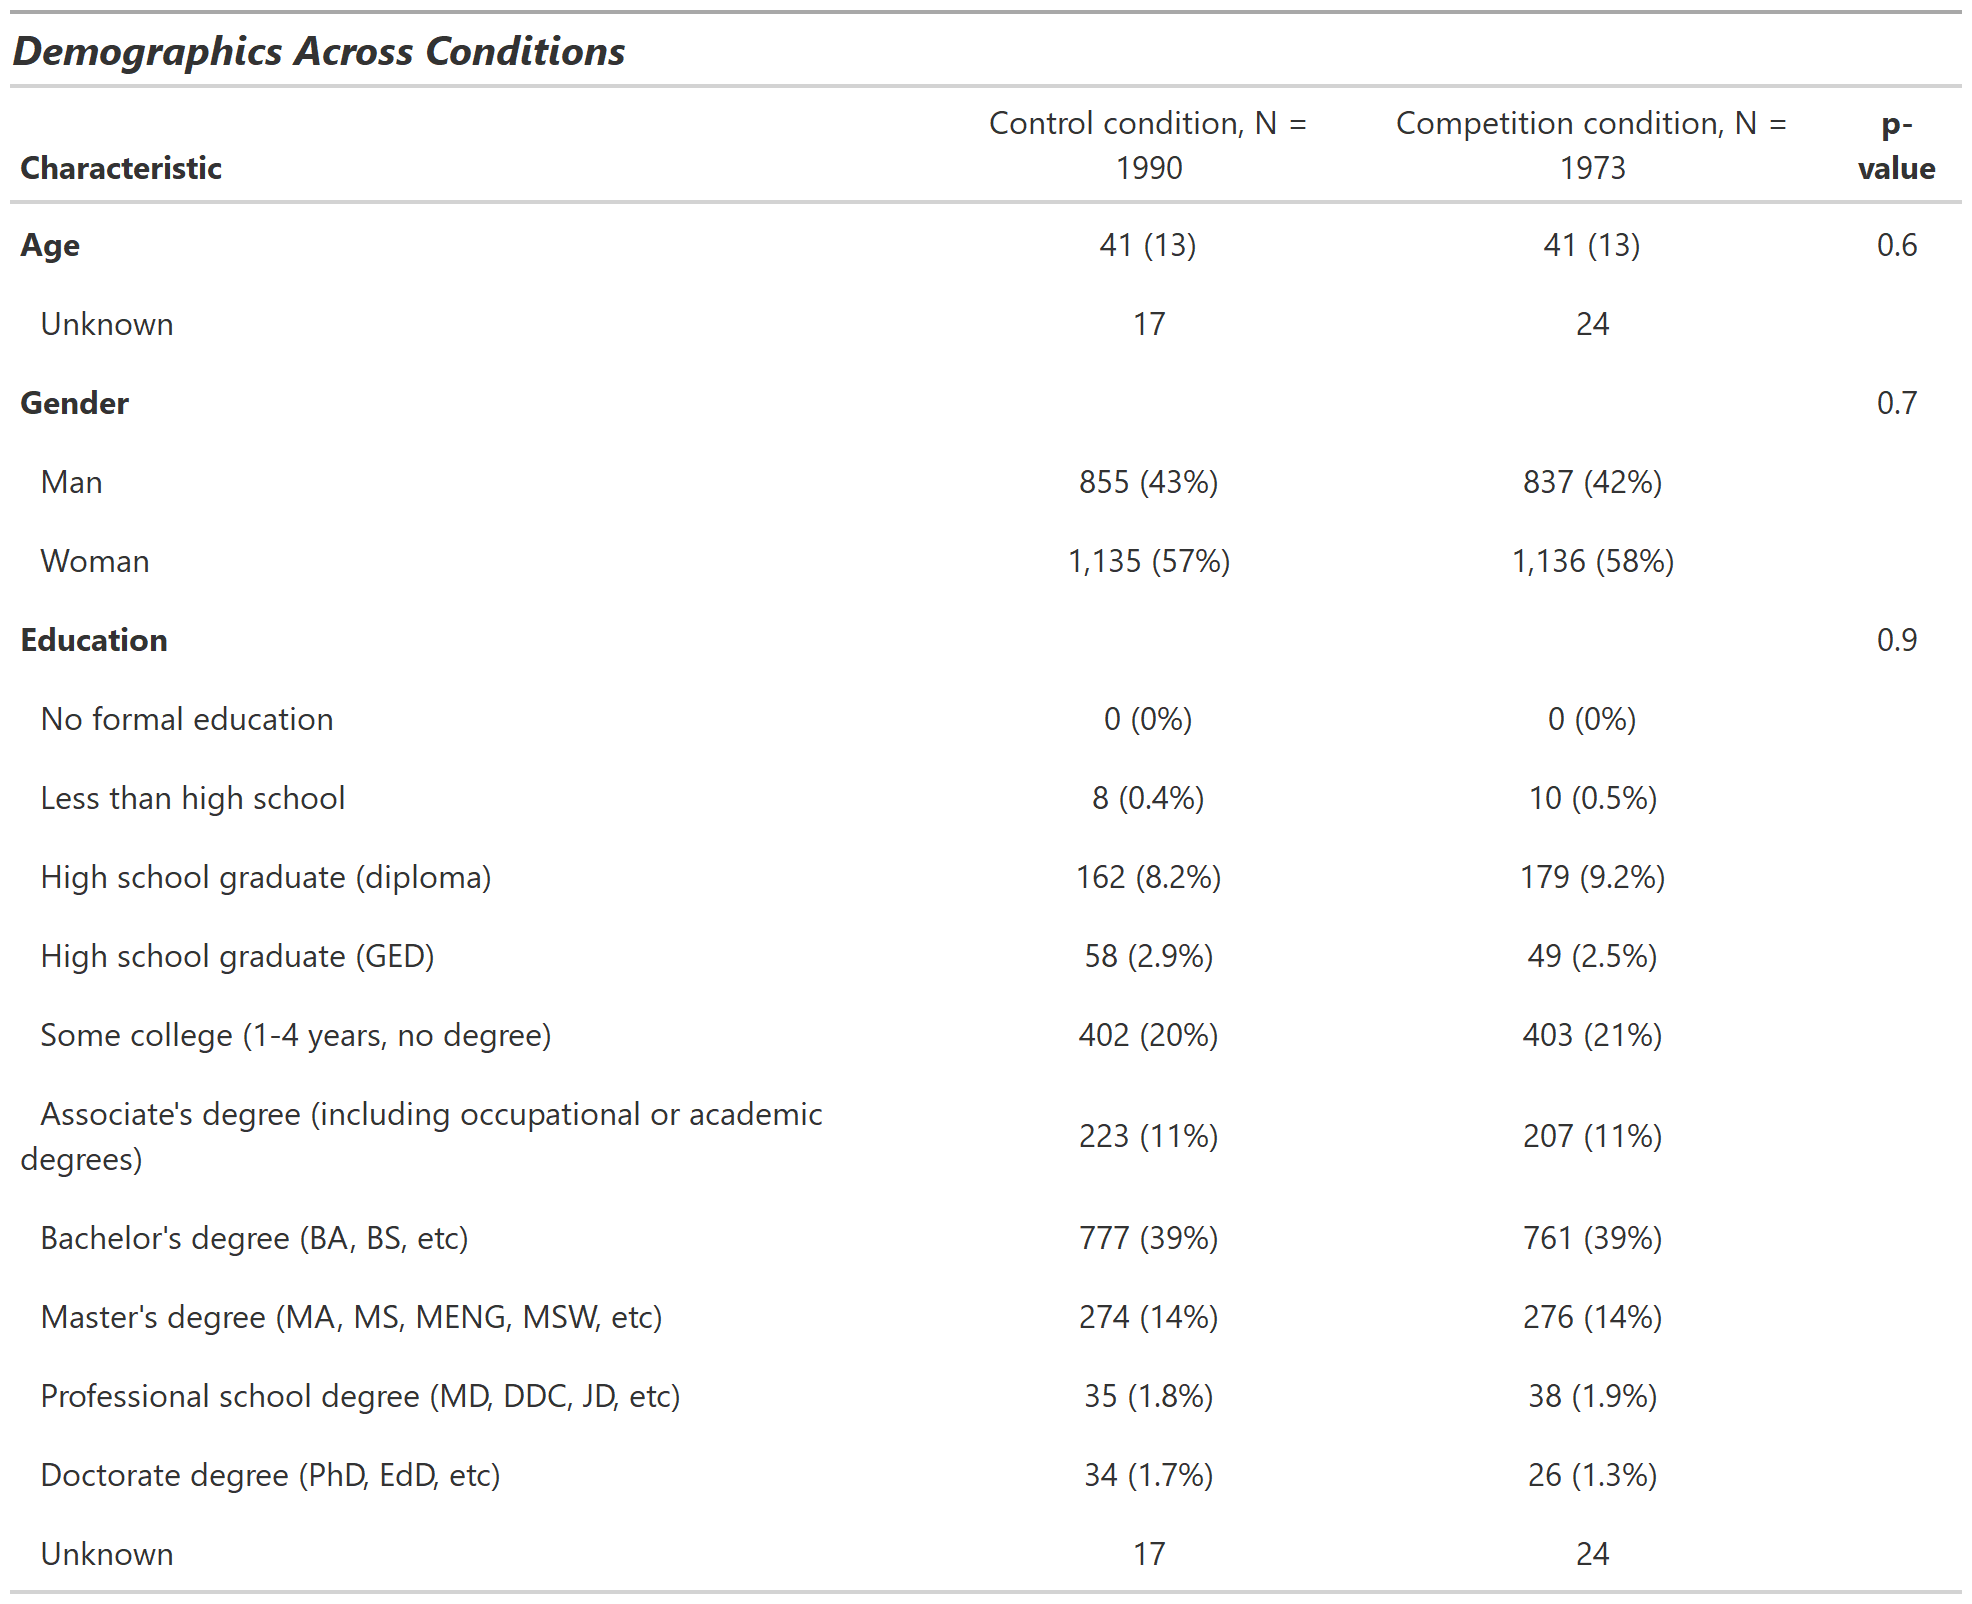
\includegraphics[width=1\linewidth]{C:/Users/keana/OneDrive - PennO365/Comp_transfer2018/Penn/practice_study/gender-practice/study5/figs/demographics-table-conds-study5} \end{center}

\begin{table}[ht]
\centering
\begingroup\fontsize{0.1pt}{0.1pt}\selectfont
\begin{tabular}{r}
   \\ 
 \end{tabular}
\endgroup
\caption{Size of sample with corresponding percentage listed for gender and education, with p-values derived from Fisher’s exact test. Mean with corresponding standard deviation listed for age, with p-values derived from Kruskal-Wallis test. If a participant did not respond to a given question, we list their response as ‘Unknown’. Note: we did not include questions about race/ethnicity nor income in this study.} 
\label{tab:demographics-table-study5}
\end{table}

\newpage

\begin{center}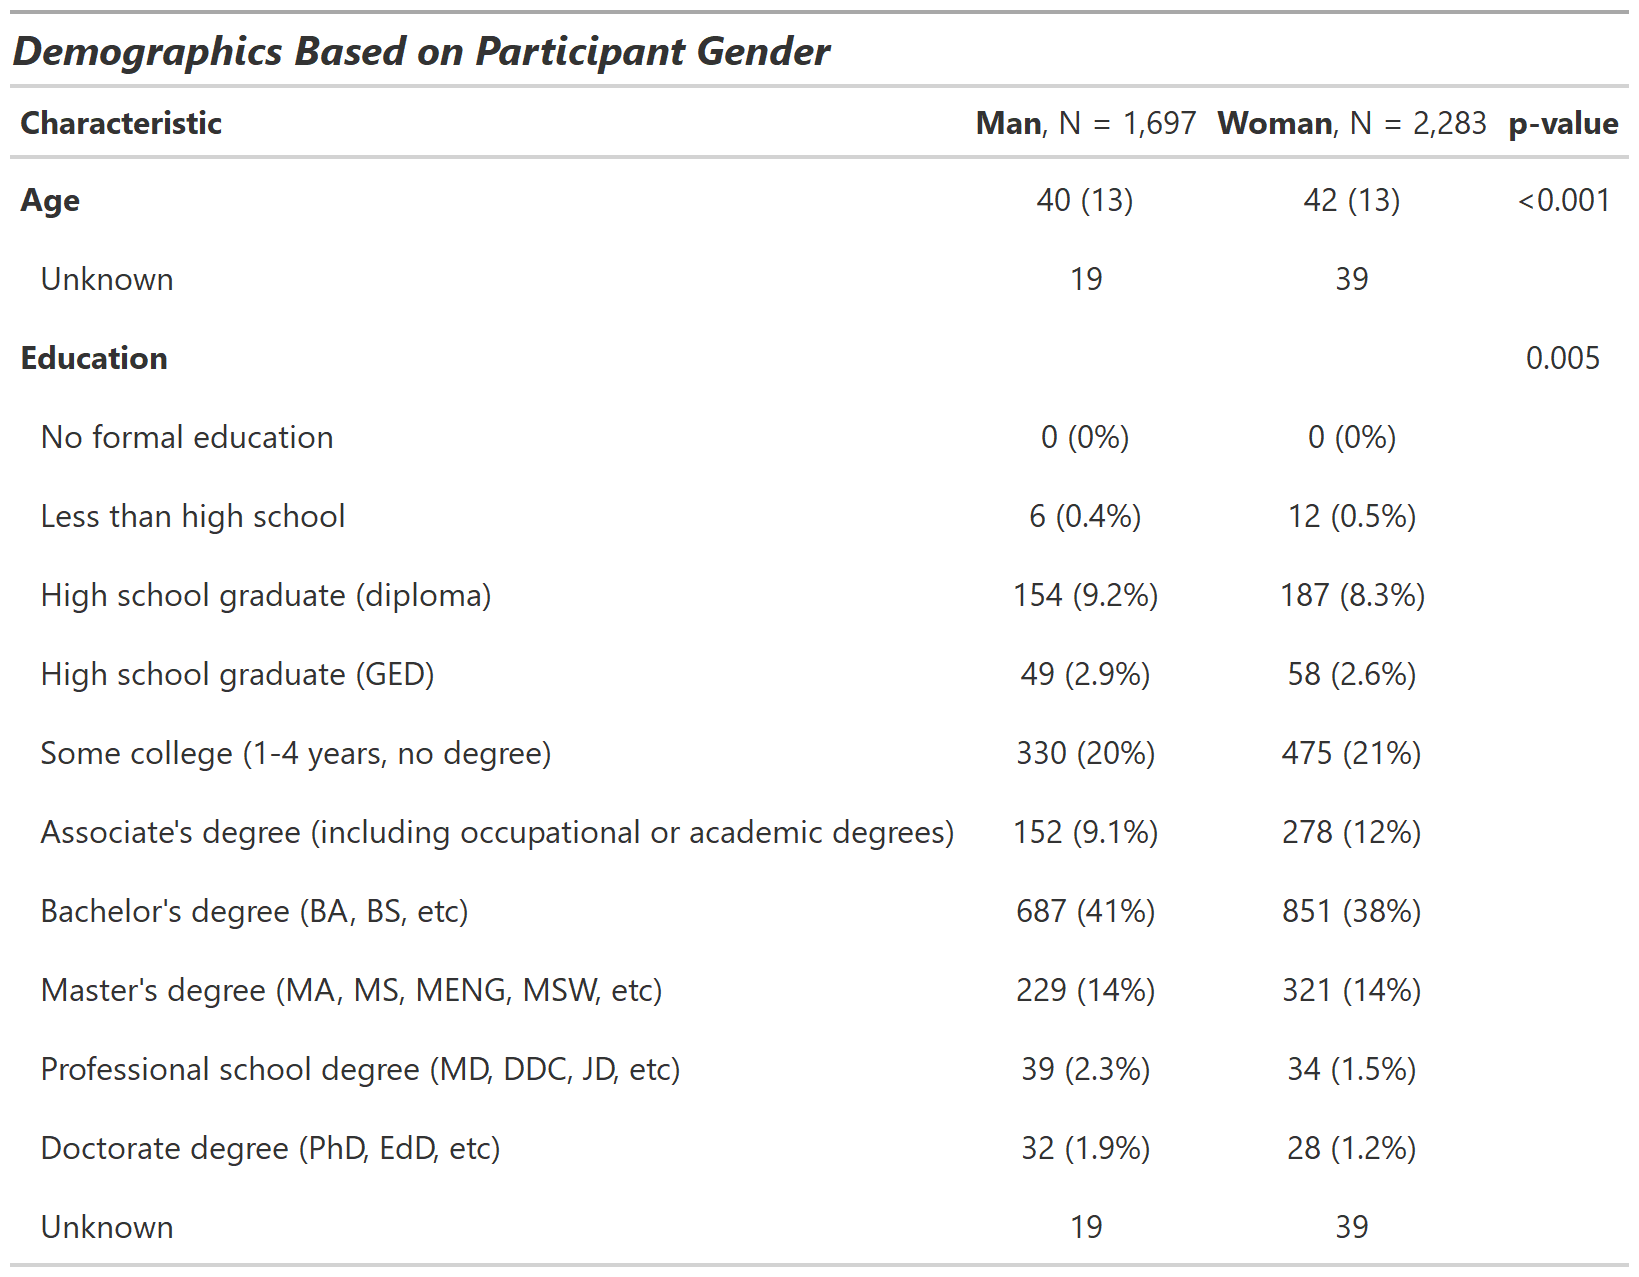
\includegraphics[width=0.85\linewidth]{C:/Users/keana/OneDrive - PennO365/Comp_transfer2018/Penn/practice_study/gender-practice/study5/figs/demographics-table-gender-study5} \end{center}

\begin{table}[ht]
\centering
\begingroup\fontsize{0.1pt}{0.1pt}\selectfont
\begin{tabular}{r}
   \\ 
 \end{tabular}
\endgroup
\caption{Size of sample with corresponding percentage listed for education, with p-values derived from Fisher’s exact test. Mean with corresponding standard deviation listed for age, with p-values derived from Kruskal-Wallis test. If a participant did not respond to a given question, we list their response as ‘Unknown’. Note: we did not include questions about race/ethnicity nor income in this study.} 
\label{tab:demographics-table-gender-study5}
\end{table}

\newpage

Given the difficulty of powering interaction effects \autocites[see][]{Simonsohn2014,Giner-Sorolla2018}, we conducted a power analysis to determine an adequate sample size for the main hypothesized interaction effect in the primary analysis \autocite[simulations modeled after code from][]{Hughes2017a}. We ran 5000 simulations while varying the sample size (\emph{N} = 3000, 3250, 3500) and the effect size for the interaction effect (\emph{b} = .2, .3, .4). Based on these simulated estimates, we aimed to recruit 4000 participants to achieve at least 80\% power for a relatively small effect (\emph{b} = .2) (see Figure \ref{fig:power-analysis-study5}). The final dataset consists of 3980 participants (57.36\% women), with an average age of 41.3 (\emph{SD} = 13.2) years. Of the final sample, 75 participants (30.67\% women) dropped out of the study before finishing (we use their data when available) and 192 participants were flagged by Qualtrics' fraud detection software as suspicious based on the aforementioned criteria.

\begin{figure}

{\centering 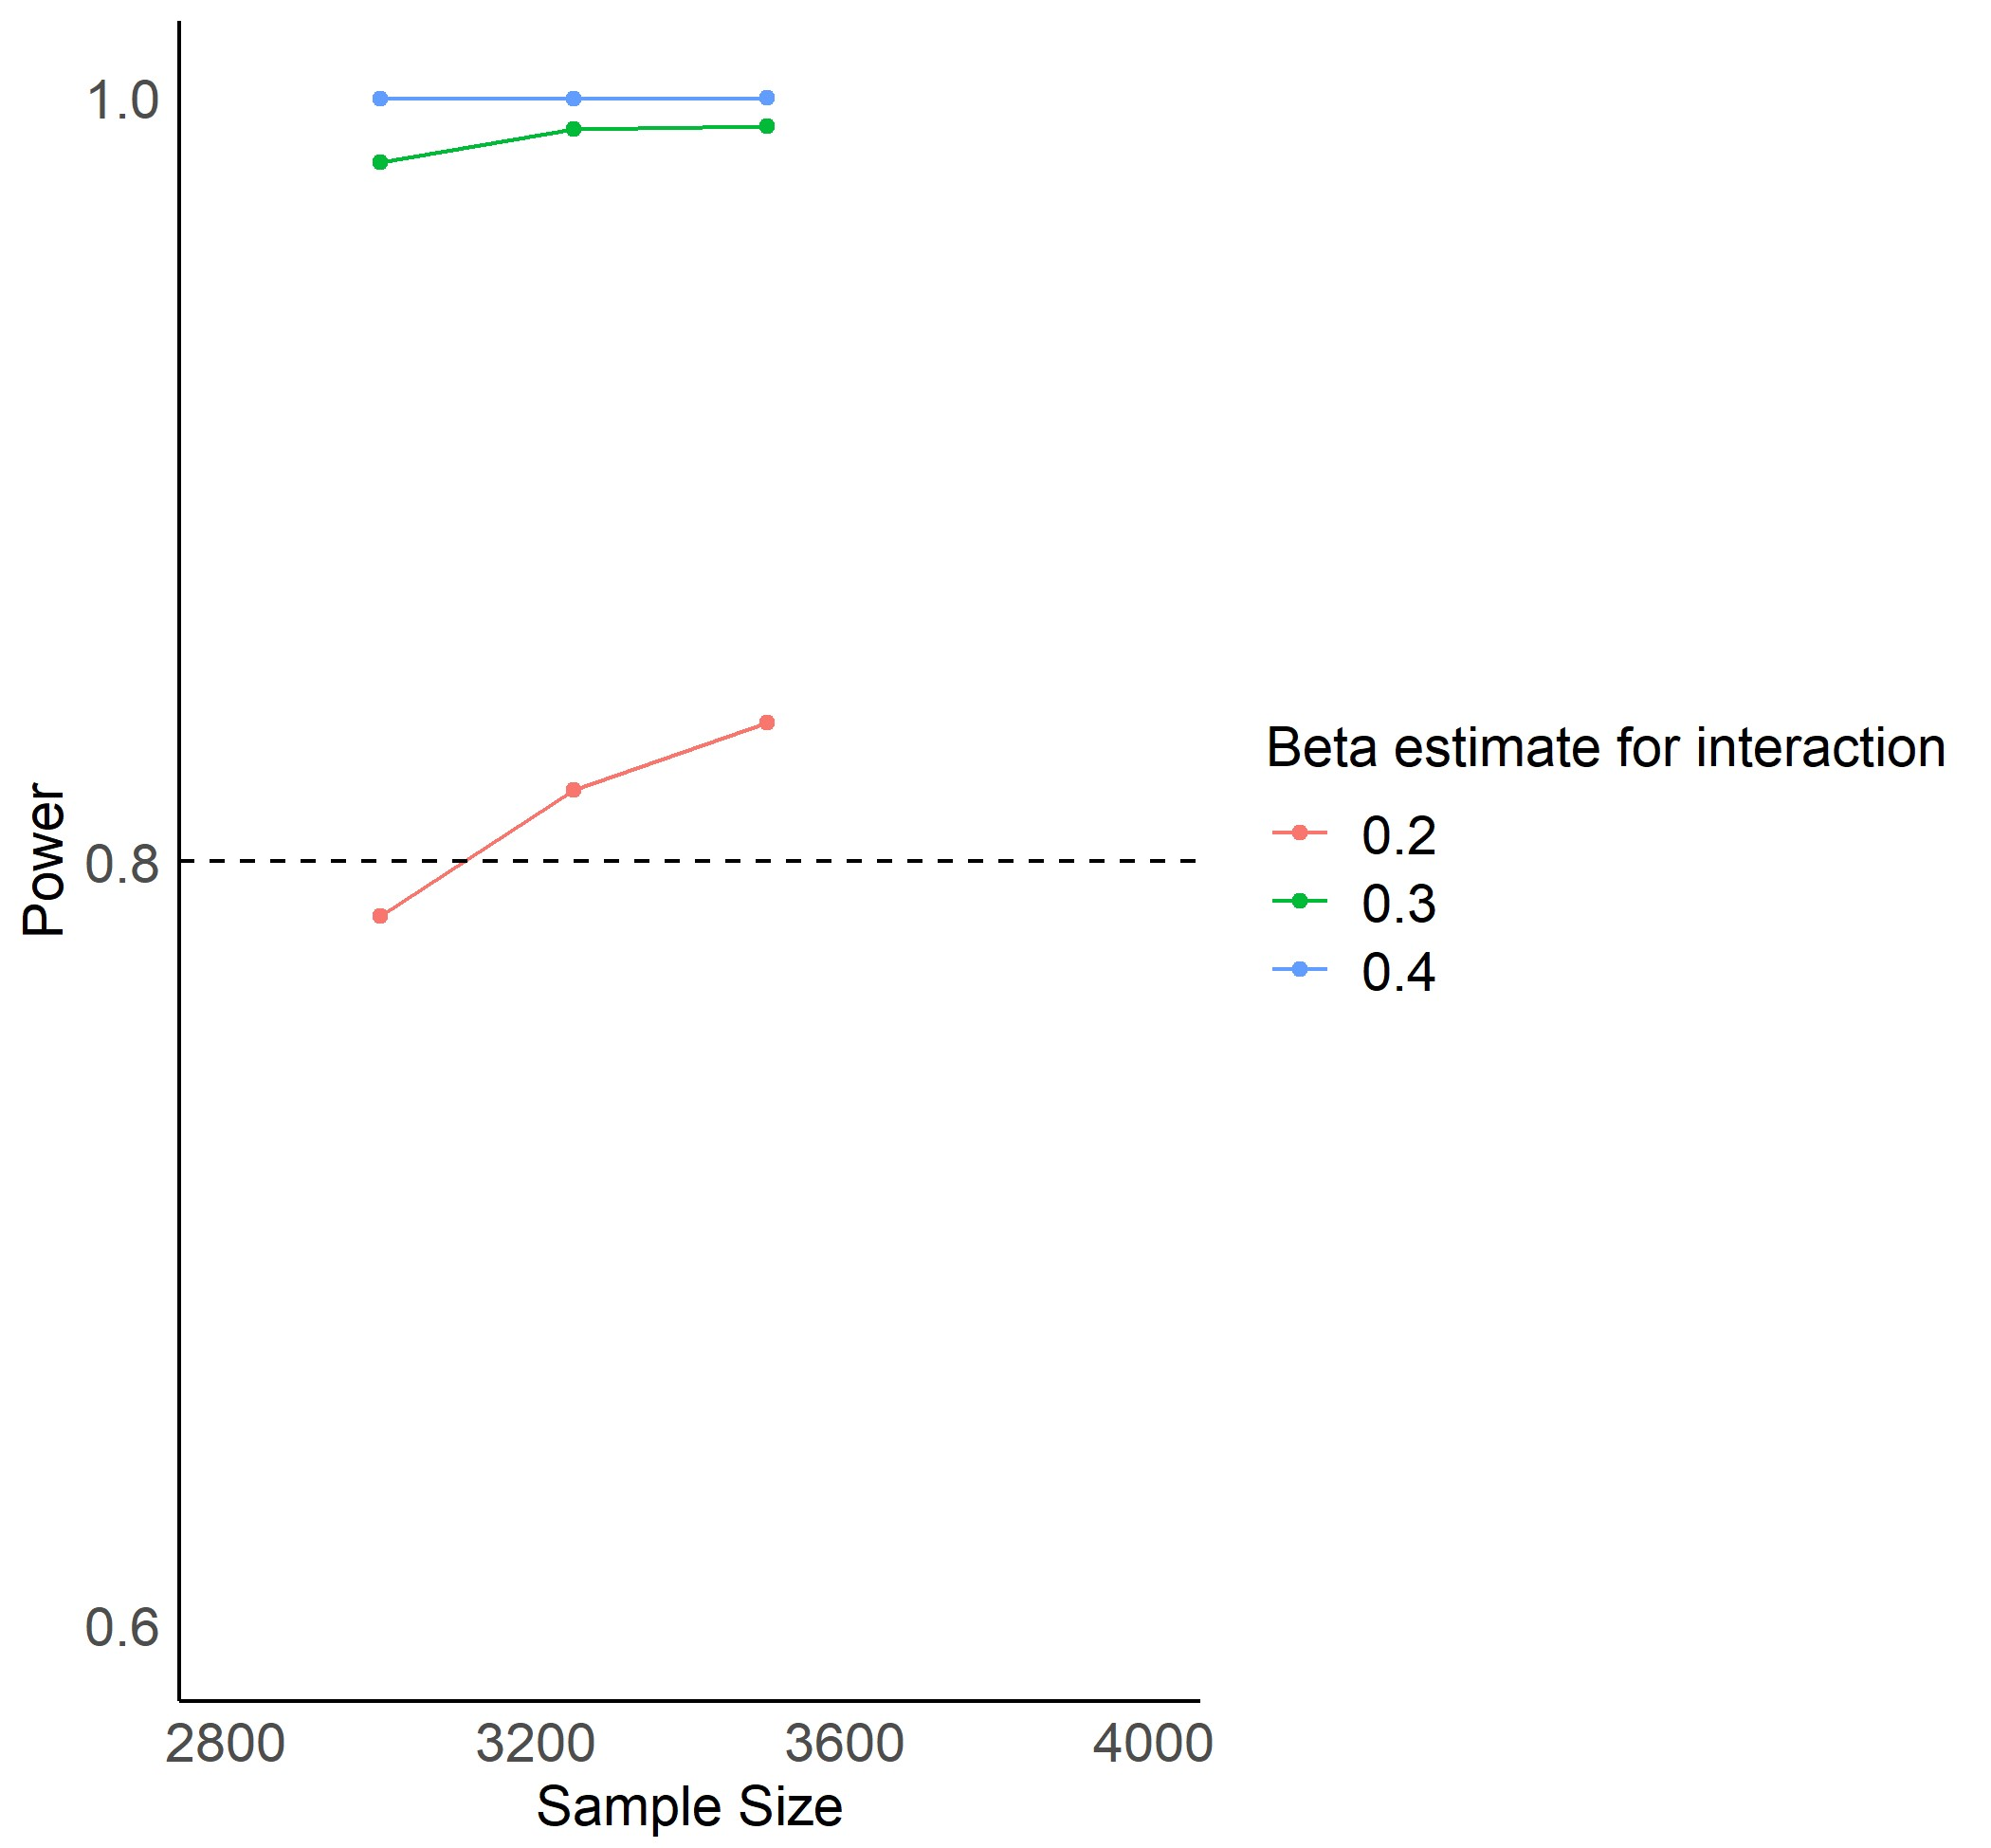
\includegraphics[width=300px]{C:/Users/keana/OneDrive - PennO365/Comp_transfer2018/Penn/practice_study/gender-practice/study5/figs/nsf-power-analysis} 

}

\caption{Plot of simulation output used to determine necessary sample size for at least 80 percent power.}\label{fig:power-analysis-study5}
\end{figure}

\hypertarget{procedures-3}{%
\subsection{Procedures}\label{procedures-3}}

Participants included in the study were told they would be completing a multiplication task. Notably, we aimed to recruit a larger sample to provide enough power to detect our anticipated interaction effects, and shortened the task from two minutes (as in Chapter 1) to 30 seconds (in the present study). Otherwise, the task used was identical to the ones used in previous studies. Like the studies in Chapter 1, participants were first told about the rules for the multiplication task and were required to pass the same comprehension questions used in the previous studies before moving onto the main manipulation of payment scheme.

\hypertarget{manipulation-of-payment-scheme}{%
\subsubsection{Manipulation of payment scheme}\label{manipulation-of-payment-scheme}}

Unlike previous studies, participants were not able to choose a payment scheme. Instead, they were told about their random assignment to one of two payment schemes: the non-competitive piece-rate payment scheme or competitive tournament payment scheme. Men and women were evenly assigned to both conditions. If they were assigned to the piece-rate payment scheme, they were paid \$.10 per problem solved correctly. If they were assigned to the tournament payment scheme, they were randomly matched with another participant that was also assigned to that payment scheme and received \$.20 per problem if they solved more problems than the other participant. Otherwise, they received nothing for their bonus payment.

Again, we checked that condition was assigned evenly across participants (control= 50.21\%) and genders included in the study. Of the men who completed the study, 50.53\% were assigned to the control condition and of the women who completed the study, 49.98\% were assigned to the control condition, \(\chi^2(1, n = 3980) = 0.10\), \(p = .754\). We also assessed condition-dependent attrition by identifying the number of participants that dropped out during/after learning about condition and found that a relatively small proportion of participants out of the total sample dropped out after learning about their respective condition (\emph{N} = 42; 0.35\% of men dropped out after learning about assigned condition versus 0.7\% of women dropped out after learning about assigned condition, \(\chi^2(1, n = 3980) = 1.14\), \(p = .285\)). Given the small sample that dropped out relative to the total number of participants in the study, we are not concerned that condition-dependent attrition is driving any of the effects found in this study.

\hypertarget{main-dependent-variables-of-interest-measures-of-preparation-and-perceptions-of-relative-preparation}{%
\subsubsection{Main dependent variables of interest: Measures of preparation and perceptions of relative preparation}\label{main-dependent-variables-of-interest-measures-of-preparation-and-perceptions-of-relative-preparation}}

After they were informed of their payment scheme, all participants were given the opportunity to spend unlimited time preparing before completing the paid multiplication task. The nature of the unlimited preparation was identical to that used in Study 3 of Chapter 1, where participants who chose to prepare were shown 10 multiplication problems that were created randomly by drawing from the pool of numbers used in the main multiplication task. Unlike the last study in Chapter 1, participants were not asked to explicitly indicate whether they would like to study the times tables. Instead, they were shown the times table right after the practice problems directly on the practice problems page and told they could check their answers using the table as desired. By including the option to check their answers, we hoped to make the practice itself more useful by providing participants a way to receive feedback on their responses. At the bottom of each practice page, participants were asked if they would like to continue practicing multiplication problems, with the option to continue as many times as desired or opt out at any point. The amount of time (in seconds) participants spent on each practice page was also recorded. Thus, like the previous studies, we have multiple measures of preparation, by design: 1) the actual decision to practice problems (before knowing what the practice entails), 2) the number of practice problems participants attempted (quantified as number of practice problems not left blank, irrespective of accuracy - with participants who did not opt into the practice having a value of zero), 3) the amount of time participants spent across all practice rounds they completed (where those who chose not to practice had a value of zero for this variable), and 4) the number of practice rounds participants completed. Since the practice structure in this study is identical to that of Study 3 in Chapter 1, the number of practice rounds variable was encoded in the same way as that study (\emph{M} = 0.59, \emph{SD} = 0.98).

After completing the practicing/studying, participants guessed how much their amount of practicing for the task compared to all other participants who completed the task by indicating the decile of their practice relative to other participants. We also asked participants to indicate their anticipated decile when their amount of practicing was compared to that of all participants who identified as men and women, respectively. We used these decile questions to create the perceived practice deviation variables as follows: self-rated decile (either based on the question about practicing relative to all other participants, relative to only men, or relative to only women) - actual percentile based on number of practice problems completed. We subtracted percentile from decile here because it provides more variation in the variable, thus allowing us to be more precise in our estimates of the effects of various predictors on this variable. We chose to ask participants to indicate their decile rather than percentile because it would be cumbersome for participants and it is unlikely they would be able to provide concise responses. Overall, negative values for this variable indicate a participant expected to have practiced less, relative to other participants, than they actually did, and vice versa for positive values.

\hypertarget{paid-multiplication-task-and-post-task-measures}{%
\subsubsection{Paid multiplication task and post-task measures}\label{paid-multiplication-task-and-post-task-measures}}

After practicing, participants completed the paid multiplication task, received feedback about their absolute (but not relative) performance, and completed many of the same follow-up questions used across Chapter 1, including risk attitudes, confidence, and perceptions of gender differences in preparation, competitiveness, and performance. Like Study 3 of Chapter 1, all questions had three response options (e.g., men are more likely to compete than women, women are more likely to compete than men, or there are no differences in how much men or women would choose to compete). One of the perceptions of gender differences questions deviated slightly from the previous studies, which was edited for the sake of clarity. Instead of asking participants to indicate ``Do you think men or women in this study chose the tournament payment option more often?'', they were asked ``If given the opportunity to choose between the two payment schemes (Piece Rate or Tournament), do you think men in this study would choose the piece rate or the tournament payment scheme more often?'', with the options to indicate: ``Men would choose tournament more often than piece rate'', ``Men would choose piece rate more often than tournament'', or ``Men would choose each payment scheme equally''. This question was repeated with respect to women in the study. We paid participants to answer the questions about their confidence and perceptions of gender differences correctly at the same rate as previous studies. Finally, they completed the same demographic questions from Chapter 1 and provided feedback on the study before being paid for their participation.

\hypertarget{results-3}{%
\section{Results}\label{results-3}}

\hypertarget{describing-main-variables-of-interest-3}{%
\subsection{Describing main variables of interest}\label{describing-main-variables-of-interest-3}}

First, we explored the characteristics of the main practice variables in the dataset. Across conditions, 45.51\% of all participants chose to practice, with 48.22\% choosing to practice in the piece-rate payment condition and 51.78\% choosing to practice in the tournament payment condition. This difference in the choice to practice across conditions is significant when condition is included as a predictor alone, \(b = 0.15\), 95\% CI \([0.02\), \(0.28]\), \(z = 2.35\), \(p = .019\), but in the subsequent section we explain how the effect changes when including other predictors in the model. Participants spent an average of 29.12 seconds practicing across all rounds of practice. We replicate the effects of gender on risk attitudes, \(b = -0.86\), 95\% CI \([-1.01\), \(-0.70]\), \(t(3920) = -10.71\), \(p < .001\), and confidence, \(b = -8.46\), 95\% CI \([-10.12\), \(-6.79]\), \(t(3978) = -9.96\), \(p < .001\) found in Chapter 1, such that women were more risk averse and less confident relative to men.

Like all studies in Chapter 1, we find a significant effect of gender on task score when included as a sole predictor, M\textsubscript{women} =10.45, SD\textsubscript{women} =4.47; M\textsubscript{men}= 12.29, SD\textsubscript{men} =7.28, \(b = -1.83\), 95\% CI \([-2.20\), \(-1.47]\), \(t(3929) = -9.75\), \(p < .001\). Contrary to the majority of studies in the first chapter, the effect of gender holds even after including risk attitudes, confidence, and an interaction between gender and condition in the model, \(b = -1.38\), 95\% CI \([-1.89\), \(-0.86]\), \(t(3916) = -5.20\), \(p < .001\) (See Table \ref{tab:tab-task-scores-study5}). We explore this finding further in the discussion section for this study. See Table \ref{tab:summary-table-gender-study5} for a summary of gender differences in the main variables of interest.

\begin{center}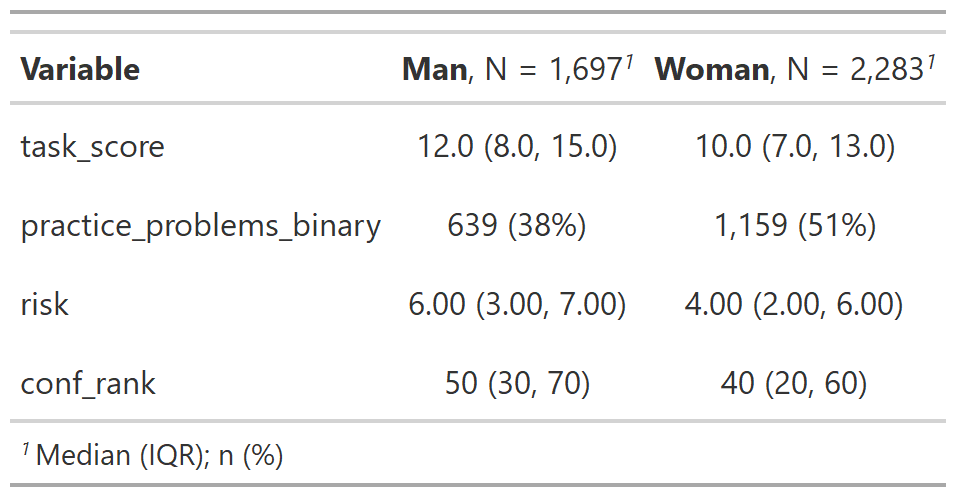
\includegraphics[width=0.5\linewidth]{C:/Users/keana/OneDrive - PennO365/Comp_transfer2018/Penn/practice_study/gender-practice/study5/figs/summary-table-gender-study5} \end{center}

\begin{table}[ht]
\centering
\begingroup\fontsize{0.1pt}{0.1pt}\selectfont
\begin{tabular}{r}
   \\ 
 \end{tabular}
\endgroup
\caption{Gender differences in the main variables of interest, including: task scores, choice to practice, risk attitudes, and confidence. Medians are reported for task score, risk attitudes, and confidence, with IQRs in parentheses. For choice to practice, we report the number and percentage of participants that fall into each category for each respective gender.} 
\label{tab:summary-table-gender-study5}
\end{table}
\newpage

\begin{center}\includegraphics[width=1\linewidth]{C:/Users/keana/OneDrive - PennO365/Comp_transfer2018/Penn/practice_study/gender-practice/study5/figs/tab_task-scores-study5} \end{center}

\begin{table}[ht]
\centering
\begingroup\fontsize{0.1pt}{0.1pt}\selectfont
\begin{tabular}{r}
   \\ 
 \end{tabular}
\endgroup
\caption{All models are linear regressions with task score as the dependent variable, where man and piece-rate payment scheme are the reference categories for participant gender and competition condition, respectively. Even after controlling for risk attitudes, confidence, and competition condition, women have lower scores on the multiplication task than men, p < .05 is considered significant and bolded.} 
\label{tab:tab-task-scores-study5}
\end{table}

\hypertarget{effects-of-gender-and-competition-condition-on-practicing}{%
\subsection{Effects of gender and competition condition on practicing}\label{effects-of-gender-and-competition-condition-on-practicing}}

We replicate the effect of gender on the choice to practice found in Chapter 1, where 51.26\% of women chose to prepare via practice, relative to 37.81\% of men, \(b = 0.55\), 95\% CI \([0.42\), \(0.68]\), \(z = 8.37\), \(p < .001\) (see right panel of Figure \ref{fig:panel-study5}). The gender effect holds in a logistic regression with gender, condition, and the interaction between the two predicting the binary choice to practice problems, \(b = 0.51\), 95\% CI \([0.33\), \(0.69]\), \(z = 5.49\), \(p < .001\) (see left panel of Figure \ref{fig:panel-study5}). However, we do not find an interaction between gender and condition, \(b = 0.08\), 95\% CI \([-0.18\), \(0.34]\), \(z = 0.60\), \(p = .547\), contrary to our hypothesis that the gender difference in the choice to prepare would be exacerbated under the tournament payment scheme relative to the piece-rate payment scheme.\footnote{The interaction between gender and competition condition on the choice to compete is still not significant among the full dataset (i.e., after including participants that were flagged by Qualtrics' fraud detection software): \(b = 0.08\), 95\% CI \([-0.17\), \(0.33]\), \(z = 0.65\), \(p = .514\). However, the effect of gender remains significant among the full dataset,} Additionally, the aforementioned effect of condition on the choice to practice is no longer significant in the model including these additional predictors, \(b = 0.10\), 95\% CI \([-0.09\), \(0.30]\), \(z = 1.03\), \(p = .302\). In a subsequent logistic regression that added confidence, risk attitudes, and task scores as predictors to explore whether they explain the gender difference in the choice to practice, we find that gender still significantly predicts the choice to practice when these variables are included in the model, \(b = 0.53\), 95\% CI \([0.34\), \(0.71]\), \(z = 5.56\), \(p < .001\) (See Table \ref{tab:tab-pract-choice-study5}).

\begin{figure}

{\centering \includegraphics[width=1\linewidth]{C:/Users/keana/OneDrive - PennO365/Comp_transfer2018/Penn/practice_study/gender-practice/study5/figs/panel_study5} 

}

\caption{Right panel shows the proportion of men and women who chose to prepare. Left panel shows the proportion of men and women who chose to prepare based on choice to compete. Women choose to prepare more than men, regardless of their decision to compete. Error bars represent standard errors.}\label{fig:panel-study5}
\end{figure}

\newpage

\begin{center}\includegraphics[width=1\linewidth]{C:/Users/keana/OneDrive - PennO365/Comp_transfer2018/Penn/practice_study/gender-practice/study5/figs/tab_pract-choice-study5} \end{center}

\begin{table}[ht]
\centering
\begingroup\fontsize{0.1pt}{0.1pt}\selectfont
\begin{tabular}{r}
   \\ 
 \end{tabular}
\endgroup
\caption{All models are logistic regressions with choice to prepare as the dependent variable, where man and piece-rate payment scheme are the reference categories for participant gender and competition condition, respectively. Women prepare more than men regardless of condition, task score, risk attitudes, or confidence. p < .05 is considered significant and bolded.} 
\label{tab:tab-pract-choice-study5}
\end{table}

We also examined other measures of practice to test the robustness of the effect of gender on practicing. We find that women, relative to men, completed a significantly higher number of practice problems, \(b = 0.39\), 95\% CI \([0.35\), \(0.43]\), \(z = 18.54\), \(p < .001\), more rounds of practice, \emph{b} = 0.31, 95\% CI {[}0.04, 0.59{]}, \emph{z} = 2.24, \emph{p} = 0.03, and spent more time completing practice problems, \(b = 13.12\), 95\% CI \([7.95\), \(18.28]\), \(t(3959) = 4.98\), \(p < .001\) while controlling for payment scheme condition and the interaction between gender and payment scheme condition. None of the interaction effects were significant across any of these dependent variables, meaning that the effects of the payment scheme conditions on the preparation outcomes did not differ by gender.

Based on previous literature on risk aversion and confidence affecting competition entry, we expected participants with especially high levels of risk aversion and/or low levels of confidence would be more likely to choose to practice before entering a competition, and that this effect may interact with gender. Thus, we tested possible three-way interactions between gender, condition, and risk aversion or confidence on the choice to practice problems through two logistic regressions, but did not find evidence that risk aversion, \(b = 0.01\), 95\% CI \([-0.10\), \(0.11]\), \(z = 0.12\), \(p = .902\), nor confidence, \(b = 0.00\), 95\% CI \([-0.01\), \(0.01]\), \(z = 0.33\), \(p = .739\), interacted with gender and condition.\footnote{Note: we run analyses with the same predictors using the other measures of preparation as dependent variables (i.e., number of practice problems completed, number of rounds of extra practice, and amount of time spent completing practice problems), and do not find evidence for interaction effects across any of those models}.

\hypertarget{perceived-levels-of-practicing-based-on-participant-gender}{%
\subsection{Perceived levels of practicing based on participant gender}\label{perceived-levels-of-practicing-based-on-participant-gender}}

Next, we ran a linear regression with gender, condition, and the interaction between those two variables predicting the aforementioned perceived practice deviation variable (that is, subtracting each participants' percentile based on number of practice problems completed from their self-rated decile) to test our second hypothesis that women would be more likely to assume they practice less than others compared to men, especially under the competitive tournament payment scheme. We find a significant effect of gender on perceived practice deviation, such that women (relative to men) were significantly less likely to assume they practice more than others, \(b = -14.49\), 95\% CI \([-19.43\), \(-9.55]\), \(t(3959) = -5.75\), \(p < .001\), M\textsubscript{women} =23.56, SD\textsubscript{women} =56.11; M\textsubscript{men} = 39.69, SD\textsubscript{men} =54.87 (see Figure \ref{fig:s410}). We do not observe a significant effect of condition on perceived relative practice, \(b = -1.30\), 95\% CI \([-6.61\), \(4.00]\), \(t(3959) = -0.48\), \(p = .630\). Finally, we did not find evidence of the anticipated interaction effect between gender and condition on perceptions of relative preparation, \(b = -3.25\), 95\% CI \([-10.26\), \(3.76]\), \(t(3959) = -0.91\), \(p = .364\).

\begin{figure}

{\centering \includegraphics[width=300px]{C:/Users/keana/OneDrive - PennO365/Comp_transfer2018/Penn/practice_study/gender-practice/study5/figs/fig02_perceived-prac-dev-by-gender} 

}

\caption{Participants' perceived practice deviation based on gender. Women had significantly lower perceived practice deviation, suggesting that they were less likely than men to overestimate their amount of practicing relative to other participants. Error bars represent standard errors.}\label{fig:s410}
\end{figure}

Since this is the first time we have used the perceived practice deviation variable and are not able to attest to its robustness, we also explored another way of testing this hypothesized effect by using participants' self-rated decile as the dependent variable instead of perceived practice deviation and then controlling for number of practice problems attempted (as a proxy for amount of practicing) in a linear regression. We find that, regardless of the number of practice problems attempted, women are significantly less likely to say they practice more than others, compared to men, \(b = -4.19\), 95\% CI \([-7.12\), \(-1.27]\), \(t(3958) = -2.81\), \(p = .005\), which aligns with the findings from the above model using perceived practice deviation as the dependent variable.

We also explored how self-rated decile changes based on whether participants were asked to compare their amount of practicing to men or women in the study specifically, and find that participants' perceptions of how much they practiced relative to women in the study are significantly lower than perceptions of much they practiced relative to men, \(M_d = -8.09\), 95\% CI \([-9.03\), \(-7.14]\), \(t(3,979) = -16.85\), \(p < .001\).

\hypertarget{perceptions-of-gender-differences-in-preparation-performance-and-competitiveness-5}{%
\subsection{Perceptions of gender differences in preparation, performance, and competitiveness}\label{perceptions-of-gender-differences-in-preparation-performance-and-competitiveness-5}}

Like in Study 3 of Chapter 1, we ran chi-square goodness of fit tests with all three response options for the questions about perceptions of gender differences, and if the test with all options was significant, we subsequently ran more targeted chi-square tests to perform pairwise comparisons. Across all measures of perceptions of gender differences in behavior, we replicate effects found in the previous studies. First, the majority of participants (59.57\%) said that women would be more likely to practice/study for the task, \(\chi^2(2, n = 3980) = 1,782.43\), \(p < .001\) (see Figure \ref{fig:s403}), which was significantly higher than the proportion of participants who said men would be more likely to practice/study than women (4.73\%), \(\chi^2(1, n = 3980) = 1,837.76\), \(p < .001\), and the proportion of participants that said there was no difference in the likelihood that men and women would practice/study (35.7\%), \(\chi^2(1, n = 3980) = 235.00\), \(p < .001\).

Similarly, participants were significantly more likely to say that women prepare more than men in general (68.28\% of participants), \(\chi^2(2, n = 3980) = 2,464.02\), \(p < .001\) (see Figure \ref{fig:s406}), relative to the proportion of participants that said men prepare more than women (4.41\% of participants), \(\chi^2(1, n = 3980) = 2,200.99\), \(p < .001\), or that there is no difference in how much men and women prepare (27.31\% of participants), \(\chi^2(1, n = 3980) = 688.84\), \(p < .001\).

Yet, participants did not expect a gender difference in performance on the main multiplication task used, \(\chi^2(2, n = 3980) = 781.11\), \(p < .001\) (see Figure \ref{fig:s404}), where 54.17\% of participants said that there was no difference in how many multiplication problems men and women correctly solved, while 20.56\% said men correctly solved more multiplication problems than women, \(\chi^2(1, n = 3980) = 594.16\), \(p < .001\), and 25.27\% said women had a performance advantage over men, \(\chi^2(1, n = 3980) = 413.36\), \(p < .001\).

Finally, 64.24\% of participants expected women would be more likely to choose the piece-rate payment scheme than the tournament payment scheme, \(\chi^2(2, n = 3980) = 1,707.40\), \(p < .001\) (see Figure \ref{fig:s408}), which was a significantly higher proportion of participants than those who expected women would choose each payment scheme equally (20.9\%), \(\chi^2(1, n = 3980) = 865.27\), \(p < .001\), and than those who expected women would choose tournament more often than piece rate, (14.86\%), \(\chi^2(1, n = 3980) = 1,209.14\), \(p < .001\). On the contrary, when asked about how much men in the study would compete, a significant majority of participants (63.5\%) expected men to be more likely to choose the tournament payment scheme over the piece-rate payment scheme, \(\chi^2(2, n = 3980) = 1,620.33\), \(p < .001\) (see Figure \ref{fig:s409}), relative to the proportion of participants who said men would choose each payment scheme equally (15.8\%), \(\chi^2(1, n = 3980) = 1,125.25\), \(p < .001\), and the proportion who said men would choose piece rate more often than tournament (20.7\%), \(\chi^2(1, n = 3980) = 853.48\), \(p < .001\). See Table \ref{tab:summary-table-beliefs-study5} for a summary of participants' responses to the questions about gender differences in preparation, performance, and competitiveness.

\newpage

\begin{center}\includegraphics[width=0.6\linewidth]{C:/Users/keana/OneDrive - PennO365/Comp_transfer2018/Penn/practice_study/gender-practice/study5/figs/summary-table-beliefs-study5} \end{center}

\begin{table}[ht]
\centering
\begingroup\fontsize{0.1pt}{0.1pt}\selectfont
\begin{tabular}{r}
   \\ 
 \end{tabular}
\endgroup
\caption{Number and percentage of participants that selected each respective option when asked whether men or women would correctly solve more problems on the multiplication task, spend more time preparing for the multiplication task, choose the tournament payment scheme more often, and spend more time preparing on most tasks. Participants were also given the option in this study to indicate there would be no gender difference for any of the variables.} 
\label{tab:summary-table-beliefs-study5}
\end{table}

\begin{figure}

{\centering \includegraphics[width=300px]{C:/Users/keana/OneDrive - PennO365/Comp_transfer2018/Penn/practice_study/gender-practice/study5/figs/fig03_perc-task-gender-pract} 

}

\caption{Proportion of participants that predicted women would spend more time preparing for the multiplication task, men would spend more time preparing for the multiplication task, or that there would be no gender differences in preparation for the task. A significantly larger proportion of participants expected women to spend more time preparing for the multiplication task. Error bars represent standard errors.}\label{fig:s403}
\end{figure}

\begin{figure}

{\centering \includegraphics[width=300px]{C:/Users/keana/OneDrive - PennO365/Comp_transfer2018/Penn/practice_study/gender-practice/study5/figs/fig06_better-gender-guess} 

}

\caption{Proportion of participants that predicted women would correctly solve more problems on the multiplication task, men would correctly solve more problems on the multiplication task, or that there would be no gender difference in performance on the multiplication task. A significantly larger proportion of participants expected there to be no gender difference in performance on the multiplication task. Error bars represent standard errors.}\label{fig:s404}
\end{figure}

\begin{figure}

{\centering \includegraphics[width=300px]{C:/Users/keana/OneDrive - PennO365/Comp_transfer2018/Penn/practice_study/gender-practice/study5/figs/fig04_perc-gen-gender-pract} 

}

\caption{Proportion of participants that predicted women prepare more in general, men prepare more in general, or that there are no gender differences in preparation in general. A significantly larger proportion of participants expected women prepare more in general. Error bars represent standard errors.}\label{fig:s406}
\end{figure}

\begin{figure}

{\centering \includegraphics[width=300px]{C:/Users/keana/OneDrive - PennO365/Comp_transfer2018/Penn/practice_study/gender-practice/study5/figs/fig05_perc-gender-comp-F} 

}

\caption{Proportion of participants that predicted women would choose the tournament payment scheme more often, women would choose the piece-rate payment scheme more often, or women would choose each payment scheme at equal rates. A significantly larger proportion of participants expected women to be more likely to choose the non-competitive piece-rate payment scheme. Error bars represent standard errors.}\label{fig:s408}
\end{figure}

\begin{figure}

{\centering \includegraphics[width=300px]{C:/Users/keana/OneDrive - PennO365/Comp_transfer2018/Penn/practice_study/gender-practice/study5/figs/fig07_perc-gender-comp-M} 

}

\caption{Proportion of participants that predicted men would choose the tournament payment scheme more often, men would choose the piece-rate payment scheme more often, or men would choose each payment scheme at equal rates. A significantly larger proportion of participants expected men to be more likely to choose the competitive tournament payment scheme. Error bars represent standard errors.}\label{fig:s409}
\end{figure}

\hypertarget{effects-of-gender-and-perceptions-on-practicing-4}{%
\subsubsection{Effects of gender and perceptions on practicing}\label{effects-of-gender-and-perceptions-on-practicing-4}}

Like all of the studies in Chapter 1, we explored whether women who believed other women prepare more were especially likely to prepare. To that end, we ran the same logistic regression with the choice to practice as the dependent variable and gender, beliefs about gender differences in preparation on most tasks, and the interaction between those two variables as the predictors. Like Study 3 of Chapter 1, the predictors representing participants' beliefs in these models had three possible values: women, men, and no difference. Like the previous studies, we focus on the interaction effect between gender and participants selecting women as the gender that spends more time preparing while controlling for all other effects in the model. We do not replicate the interaction effect found in the previous studies, such that women who said women generally prepare more on most tasks were not significantly more likely to prepare, \(b = -0.18\), 95\% CI \([-0.83\), \(0.46]\), \(z = -0.54\), \(p = .587\) (see Figure \ref{fig:pract-choice-by-gender-and-perc-gen-prep-bar-study5}). Instead, we find a main effect of gender on choice to prepare across the response options, such that women prepared more than men regardless of whether they thought women prepared more on most tasks, men prepared more, or there was no gender difference in preparation, \(b = 0.70\), 95\% CI \([0.08\), \(1.33]\), \(z = 2.20\), \(p = .028\). We ran the same analysis with participants' beliefs about gender differences in preparation for the multiplication task, gender, and the interaction between the two as predictors instead, and replicate the interaction effect from the previous studies, \(b = 1.02\), 95\% CI \([0.42\), \(1.63]\), \(z = 3.34\), \(p = .001\), such that women who expected women to spend more time preparing for the multiplication task were especially likely to prepare (see Figure \ref{fig:pract-choice-by-gender-and-perc-task-prep-bar-study5}).

\begin{figure}

{\centering \includegraphics[width=300px]{C:/Users/keana/OneDrive - PennO365/Comp_transfer2018/Penn/practice_study/gender-practice/study5/figs/pract-choice-by-gender-and-perc-gen-prep-bar-study5} 

}

\caption{Proportion of men and women who chose to practice based on whether they thought men or women spend more time preparing on most tasks. In this study, participants also had the option to say there was no gender difference in preparation. Women who thought women generally prepare more were not especially likely to choose to practice. Error bars represent standard errors.}\label{fig:pract-choice-by-gender-and-perc-gen-prep-bar-study5}
\end{figure}

\begin{figure}

{\centering \includegraphics[width=300px]{C:/Users/keana/OneDrive - PennO365/Comp_transfer2018/Penn/practice_study/gender-practice/study5/figs/pract-choice-by-gender-and-perc-task-prep-bar-study5} 

}

\caption{Proportion of men and women who chose to practice based on whether they thought men or women spend more time preparing for the multiplication task. In this study, participants also had the option to say there was no gender difference in preparation. Women who thought women prepare more for the multiplication task were especially likely to choose to practice. Error bars represent standard errors.}\label{fig:pract-choice-by-gender-and-perc-task-prep-bar-study5}
\end{figure}

\hypertarget{discussion-3}{%
\section{Discussion}\label{discussion-3}}

\hypertarget{summary-of-main-experimental-results-3}{%
\subsection{Summary of main experimental results}\label{summary-of-main-experimental-results-3}}

First, we find that, like previous literature in this space and our own studies across Chapter 1, women are more risk-averse and less confident than men in this study. Yet, even when controlling for gender differences in risk attitudes and confidence, we replicate findings from the studies in Chapter 1 that women choose to prepare more than men. Interestingly, women chose to prepare more regardless of the payment scheme (competitive tournament, non-competitive piece-rate) they were randomly assigned to. Also, although participants overall were more likely to practice in the tournament scheme, we did not find evidence that assignment to either a tournament or piece-rate payment scheme significantly predicted the binary choice to practice problems, after including gender and the interaction between gender and condition in the model. Although we did not explicitly hypothesize a priori that condition would be a significant predictor of the choice to practice, it is nonetheless important to note that gender explains participants' decision to practice problems over and above any effect of competition condition.

We also included other means of quantifying preparation (i.e., amount of time spent on the pages with practice problems and study tables, number of practice problems completed, and total number of practice rounds completed) to test the robustness of the gender effect, and find evidence across our multiple measures of preparation that women tended to prepare more than men-- they spent more time completing practice problems and studying tables, completed a higher number of practice problems, and completed more rounds of practice.

One important consideration when interpreting the effect of gender on the choice to prepare before the task is that, contrary to our prior studies (Chapter 1), we find a significant effect of gender on task score, even while controlling for individual differences in risk attitudes and confidence, unlike two out of the three studies in the last chapter. It is possible that shortening the task contributed to this effect - especially considering evidence suggesting that women's performance may suffer under more competitive pressure \autocite{Gneezy2003,Gneezy2004,Gunther2010,Samak2013,Booth2022,Gneezy2004,Niederle2011,Cotton2013}. There may be less pressure to perform well during a two-minute task (used in all of the studies of Chapter 1) relative to a 30-second task (used in the study in this Chapter). In support of this possibility, \textcite{Shurchkov2012} shows that womens' performance significantly improves, to the extent that they outperform men, in a low time pressure competition.

We also found evidence for the hypothesized main effect of gender in our other primary pre-registered analysis, where women were more likely to assume they practice less than others compared to men. This effect held when using our pre-registered version of the analysis using the perceived practice deviation variable, representing the accuracy of participants' guess of how much their level of practicing compared to others participants' level of practicing. We also tested the robustness of the effect using a slightly different way of quantifying our relationship of interest, where we included participants' raw self-reported practice decile as the main dependent variable of interest (instead of perceived practice deviation) with gender and number of practice problems attempted as predictors. We replicate the aforementioned effect, where women tended to think they practice less than others, regardless of how many practice problems they actually attempted.

We did not find the hypothesized interaction between gender and condition on perceived practice deviation - suggesting that, like actual decisions to practice, women's tendency to perceive they are practicing less than others is not significantly affected by whether they are competing or not. Although it is not possible to draw strong conclusions from null effects, we explore possible reasons for the null interaction between gender and condition further in the subsequent general discussion summarizing results across all studies of the dissertation.

\hypertarget{perceptions-of-gender-differences-in-preparation-performance-and-competitiveness-6}{%
\subsection{Perceptions of gender differences in preparation, performance, and competitiveness}\label{perceptions-of-gender-differences-in-preparation-performance-and-competitiveness-6}}

With respect to the questions asking participants to indicate their perceptions of gender differences about our main behavioral variables of interest, we replicate findings from all three studies in Chapter 1. Even though participants expected that women and men would not have a significant difference in task scores, they expected men to prefer the tournament payment scheme over the piece-rate payment scheme, while expecting women to both i) prefer the piece-rate payment scheme over the tournament payment scheme and ii) prepare more, both before completing the multiplication task used in this study and in general before most tasks. Again, with the exception of the general gender difference in practice questions, all of the other perception questions were incentivized for accuracy to reduce socially desirable responding. Our exploratory analysis of the new set of questions about perceptions of relative practicing compared to each gender included in the study of this Chapter support these general perceptions of gender differences in preparation. Given the targeted nature of the questions, we were able to test how participants' responses changed based on whether they were asking to compare their level of practicing in the study to only participants that identified as women or only participants that identified as men, and find that participants were significantly more likely to indicate that they practiced less relative to women than relative to men.

On top of the gender differences in practicing and perceptions of said gender differences, we again explored whether these perceptions aligned with individuals' practicing behaviors. We have mixed evidence for the hypothesized effect in this study, such that women were especially likely to prepare for the task if they believed that women prepare more than men for the multiplication task, but preparation behavior did not seem to be related to their beliefs about gender differences in preparation on most tasks.

\hypertarget{summary-3}{%
\subsection{Summary}\label{summary-3}}

Overall, our results for the study in Chapter 2 suggest that women prepare more than men, regardless of whether they were assigned to a competitive tournament or non-competitive piece-rate payment scheme, and despite thinking they practice relatively less than men for the multiplication task used in the study. It is possible that gender stereotypes are driving these gender differences in behaviors and perceptions, given our replication of the findings from all three studies in Chapter 1 that participants expected women to prepare more both before the specific task used in the study and in general, along with the finding that participants tended to rate their relative practicing significantly lower when comparing themselves to women than men. In our direct test of the relationship between participants' perceptions of gender differences in behavior and their choice to prepare, we find that women are only more likely to prepare when they believe that women prepare more than men for the multiplication task, but their perceptions of general gender differences in preparation behaviors is not strongly related to their choice to prepare. We discuss these findings in light of the full set of results in the overall discussion section.

\hypertarget{chapter-4-discussion}{%
\chapter{Chapter 4: Discussion}\label{chapter-4-discussion}}

\adjustmtc
\markboth{Discussion}{}

\hypertarget{summary-of-main-results-across-studies}{%
\section{Summary of main results across studies}\label{summary-of-main-results-across-studies}}

When considered in general, the results of this research suggest that women prepare more than men before performing, regardless of whether they were being compensated based on individual performance (piece-rate) or relative to another individual (competition). And the novel gender difference in preparation discovered in this study aligns with participants' beliefs about gender differences. Given the effects of stereotypes and beliefs about identity-based behavior on one's own behavior \autocite{Bordalo2019,Miller2016,Ellemers2018,Akerlof2000,Benjamin2010c}, stereotypes may be contributing to gender differences \footnote{Though it is important to flag here that these results were not tested through an experiment, so we cannot directly attest to causality. See Future Research section for suggestions on testing causal effects of gender stereotypes on behavior.}, both in preparation observed in this study and competitiveness observed in the literature. In fact, the effects found with regards to gender stereotypes are more robust (that is, replicated across more studies) than the actual gender difference in preparation. Importantly, opportunities to prepare (in various forms) do \emph{not} affect women's willingness to compete. In the subsequent sections, we highlight the main findings that we replicate across studies, along with some study-specific findings.

\hypertarget{effects-of-preparation-conditions-in-chapter-1-on-gender-differences-in-the-choice-to-compete}{%
\subsection{Effects of preparation conditions in Chapter 1 on gender differences in the choice to compete}\label{effects-of-preparation-conditions-in-chapter-1-on-gender-differences-in-the-choice-to-compete}}

We employed three manipulations of the opportunity to prepare in the studies of Chapter 1. First, the knowledge of preparation condition in Study 1 was a way to see if simply knowing about the opportunity to prepare, without experiencing it directly, would reduce the gender differences in the choice to compete. However, we found no evidence of effects of that manipulation on gender differences in competitiveness. Therefore, in Study 2 we tested whether the act of experiencing preparation firsthand through limited preparation for a predetermined number of rounds would affect the gender gap in competitiveness. We expected that seeing the improvement in one's performance over time may have been the key to increasing women's competitiveness. Since the manipulation of preparation in a limited capacity did not show effects on the gender difference in competitiveness in Study 2, we explored unlimited preparation as our opportunity to prepare manipulation in Study 3. One could argue that participants in the limited preparation condition may have felt like they were not getting any additional preparation above and beyond what other participants were receiving because they could not choose how much they prepared, and thus, they did not feel like the preparation would have helped their performance substantially more than it would have helped other participants. Therefore, the unlimited preparation manipulation may have helped participants who took advantage of the opportunity feel as though they had a chance to improve their performance far more than other participants, making them more willing to compete. Yet, we did not find effects of the unlimited preparation condition on gender differences in competitiveness in Study 3 either. Overall, across all three studies in Chapter 1, we do not find evidence that preparation increases men or women's willingness to compete, despite finding evidence in Study 3 of Chapter 1 that participants believe practicing helps performance on the main task both based on their behavior and their responses to the manipulation check question. Thus, we do not find evidence that any forms of preparation used in the studies of Chapter 1 would serve as a viable intervention to increase women's competitiveness.

\hypertarget{does-gender-predict-preparation-and-tests-of-robustness-of-gender-effect}{%
\subsection{Does gender predict preparation? And tests of robustness of gender effect}\label{does-gender-predict-preparation-and-tests-of-robustness-of-gender-effect}}

Despite the lack of evidence for the effect of preparation on gender differences in the choice to compete, we discovered a sizable gender difference in preparation across multiple measures of preparation, where women choose to prepare more often than men in three out of the four studies in the dissertation. Interestingly, we do not find evidence across any of the studies that the gender difference in preparation varies based on whether participants are competing, either by choice (Chapter 1 studies) or random assignment (Chapter 2 study) - that is, there is not a significant interaction between gender and the payment scheme participants were following across any of the studies. However, we find that being in a competitive environment by itself (whether by choice or not) reliably predicts the decision to prepare, regardless of participant gender.

Across studies, preparation was operationalized in several ways (i.e., choice to practice multiplication problems, choice to study times tables, amount of time spent studying times tables). The effect of gender on preparation was most robust with the measure of preparation representing the choice to prepare, which was the most consistent measure of preparation used across all four studies of the dissertation. Importantly, the observed gender differences in the choice to practice are not explained by gender differences in risk, confidence, or task scores. Because risk, confidence, and task scores were measured after participants practiced, risk and confidence could still predict decisions to practice so we encourage future research to explore this possibility.

Finding the effect of gender on the decision to prepare is especially noteworthy because we are drawing from a participant pool (MTurk) where participants could be earning money for their participation through a nearly limitless supply of other studies, so the opportunity costs of preparing may be greater for MTurkers relative to other participant populations, suggesting that this effect could be even stronger when the opportunity costs are lower.

Importantly, across two out of the four studies, we find no gender difference in task performance when controlling for gender differences in risk attitudes and confidence, so the gender difference in the decision to prepare does not seem to be consistently driven by gender differences in the actual need to practice. In the Chapter 2 study, where we find a gender difference in performance on the multiplication task, we argue that one possible reason we find the gender difference was the use of a shortened task (30 seconds instead of two minutes), given previous research suggesting that gender differences in performance emerge under time pressure \autocite{Shurchkov2012}.

To our knowledge, these studies are the first to demonstrate a gender difference in preparation among adults who must explicitly opt into preparation. However, previous findings within educational contexts have found that women are more likely than men to value dedication and mastery \autocite{Leslie2015,Kenney-Benson2006}, emphasize the importance of hard work \autocite{Mccrea2008,Hirt2009,Mccrea2008a}, and spend more time preparing than men for an intellectual evaluation when they were told that practice improved future performance \autocite{Kimble2005}. For instance, in a study examining school-aged children's approach to learning math, researchers found that girls, compared to boys, reported being more motivated to ``master'' their schoolwork and engage in more effortful learning strategies \autocite{Kenney-Benson2006}. \textcite{Becker2010} suggest that women have higher noncognitive skills (e.g., self-motivation) than men along many dimensions, which they argue is reflected in gender differences in a number of academic behaviors and outcomes, such as grades and number of hours worked on homework per week. In one study looking at whether delaying competition affects gender differences in the willingness to compete while providing opportunity to study, \textcite{Charness2021} did not find a significant difference in the choice to prepare (\emph{N} = 202). Although it is worth noting that, though the effect is non-significant, women are directionally more likely to prepare in their study. Since studying gender differences in the choice to prepare was not one of the main foci of their research, contrary to ours, it is entirely possible they did not have sufficient power to detect the effect of gender on the choice to prepare as a result.

In a similar vein, there has been a burgeoning set of research results in recent years suggesting that there are gender stereotypes about brilliance or raw talent, such that women are perceived as less likely to be brilliant or exhibit less raw talent than men, which in turn affects their decisions, preferences, and representation across fields \autocite{Bian2017,Bian2017a,Leslie2015,Meyer2015,Bian2018,Storage2020}. \textcite{Napp2022} performed an investigation among 500,000 students across 72 countries to test whether the ``gender-brilliance'' or ``gender-talent'' stereotype 1) exists internationally and 2) translates to other gender gaps known to be important for gender differences in economic outcomes (i.e., competitiveness, confidence, and willingness to enter certain careers). Based on participants' responses to their measure of the gender-talent stereotype (i.e., testing systematic gender differences in response to a survey question asking ``When I am failing, I am afraid that I might not have enough talent.''), they find evidence for both of their hypothesized effects. That is, they find that the gender stereotype is present across countries and the strength of the gender-talent stereotype is related to the size of gender gaps in competitiveness, confidence, and willingness to enter male-dominated careers that are stereotyped to require raw talent for success. They note that the gender-talent stereotype does not lead girls to feel as though they should not put effort towards other, perhaps less competitive, domains, where girls are in fact more likely than boys in the study to agree with the sentiment ``if I put in enough effort, I can succeed at school.'' They argue that their findings overall suggest that the gender-talent stereotype is not all-encompassing, such that the stereotype will not affect women and girls' behaviors and preferences in environments that do not fall into male-typed domains. Thus, the gender-talent stereotype may be one factor contributing to the gender difference in preparation, driven by the belief that women lack as much talent as men, and as such, may need to compensate for their lack of talent in environments that are male-typed. Importantly, they also note that the gender-talent stereotype can in some cases have negative consequences for men, such that they may rely too heavily on talent, and end up exerting less effort, leading to lower performance during bouts of sustained effort such as studying or longer cognitive tests \autocite{Balart2019}. Overall, the literature on the gender-talent stereotype is highly relevant to the current dissertation, and we encourage future research to explore how our findings may relate to said stereotype (see Future Directions section).

\hypertarget{possible-reasons-for-study-3-deviation}{%
\subsubsection{Possible reasons for Study 3 deviation}\label{possible-reasons-for-study-3-deviation}}

Notably, we do not replicate the effect of gender on the choice to practice problems in Study 3 of Chapter 1. Although we cannot be completely certain what may be underlying our inability to replicate the effect found in the other studies of the dissertation, we describe a few possible explanations here. First, all other studies in the dissertation measured the decision to complete practice problems \emph{after} participants chose to (or in the case of the study in Chapter 2, were randomly assigned to) compete, while Study 3 measured the decision to practice problems \emph{before} the decision to compete, as necessitated by the main manipulation within the study. Thus, the differences in the results across studies could be explained by the effects of the decision to compete on the choice to practice that are not captured in Study 3. In other words, not knowing they might not have to compete could have reduced motivation to practice. There are also fewer participants that are offered the opportunity to practice in Study 3 (N = 531) relative to Study 1 of Chapter 1 (N = 1044), Study 2 of Chapter 1 (N = 1071), or the study in Chapter 2 (N = 3963), again by nature of the study design (i.e., manipulating unlimited opportunity to prepare) so Study 3 likely had less power to detect the effect than the other studies. Finally, the structure of practicing itself was different in Study 3 relative to the other studies. The other studies in the dissertation did not offer participants the opportunity to study multiplication tables as a separate decision from the choice to practice problems, whereas in Study 3 of Chapter 1, participants were first asked whether they would like to study multiplication tables, \emph{then} afterwards were asked whether they would like to practice problems. Perhaps being asked whether they would like to study before being asked whether they would like to practice problems reduced participants' interest in completing practice problems. Notably, regardless of what might be explaining the deviation for this study, we do not find evidence across any of the studies nor any of the measures of preparation that men are significantly or even directionally more likely to prepare than women.

\hypertarget{possible-explanations-for-the-gender-difference-in-preparation}{%
\subsubsection{Possible explanations for the gender difference in preparation}\label{possible-explanations-for-the-gender-difference-in-preparation}}

The gender difference in preparation observed in the majority of the studies here may be driven by women's relatively greater desire to reduce uncertainty around their future performance (given their greater average risk aversion) and/or increase their performance (given their lower average confidence). Indeed, mastery is an important driver of confidence \autocites[for review, see][]{Gist1992,Usher2008}. While it is possible that confidence and risk attitudes may be driving the gender difference in preparation and the choice to compete, it is important to note that preparation in our studies did not increase competitiveness in either men or women. Because participants were able to choose to prepare across studies before they completed the measures of risk attitudes and confidence, we are unable to identify whether preparation causally affected confidence and/or risk attitudes. Future work should examine the bidirectional relationships between confidence and preparation and risk and preparation. Of course, other explanations for the gender differences in preparation may also exist, including relative differences in real or perceived opportunity costs, how rewarding it is to prepare, and/or enjoyment on the task, and we encourage future work to explore these alternative explanations. Notably, given the consistency of perceptions of gender differences in preparation found across studies, our results directly speak to another possible explanation for the observed gender difference in preparation: stereotypes that women prepare more than men in general. In fact, gender stereotypes about preparation may be one of the reasons we did not find evidence for the hypothesized interaction between gender and payment scheme on the choice to prepare across any of the studies. Specifically, gender stereotypes about preparation may be so powerful that women prepare more than men regardless of context. Since we collected data both about the choice to prepare and perceptions of gender differences in preparation across all studies in the dissertation, we could directly test whether gender and beliefs about gender differences in preparation were related to the choice to prepare. We find evidence across multiple studies that gender stereotypes are in fact related to preparation, such that women were especially likely to prepare when they believed women prepare more both in general and for the multiplication task. However, we reiterate the importance of testing these effects causally, especially since we are unable to test the directionality of the relationship between perceptions of gender differences and gender differences in behavior in these studies. That is, practicing may have led participants' to believe that other individuals who have the same gender identity practice more (behavior leading to perception) or the belief that other participants who have the same gender identity practice more may have led participants to practice more (perception leading to behavior). As such, we implore future research to explore these questions through experiments. Finally, we found evidence of a gender difference in performance on the task in two of the four studies. As preparing may have helped performance, it is possible that the gender difference was fully explained by gender differences in the need to prepare on the task. Since our research is not able to directly test whether the choice to prepare was driven by the actual need to prepare based on performance, we encourage future research to explore the possibility that gender differences in performance may have been driving the gender difference in preparation by employing less gender-typed tasks (see Future Directions section).

\hypertarget{summary-of-effects-of-perceptions-of-gender-differences}{%
\subsection{Summary of effects of perceptions of gender differences}\label{summary-of-effects-of-perceptions-of-gender-differences}}

On top of the gender differences in preparation observed, we find that participants \emph{believe} that women prepare more, both in general and on the multiplication task (incentivized for accuracy) across all four studies. Thus, participants accurately predicted the observed gender differences in preparation, suggesting that they observe these gender differences in preparation directly in their own lives and/or have learned stereotypes surrounding gender differences in preparation. There is extensive work suggesting that beliefs about identity-based behavior and social norms affect subsequent behavior \autocite{Babcock2012,Bowles2007,Toosi2019,Smith2014,Benjamin2010c,Bertrand2015,Akerlof2000}. One possibility is that women may be preparing more because these beliefs may indirectly make women feel like they are expected to prepare more, and as a result, women may be overpreparing (relative to their actual skill level) before performing. If future work confirms this hypothesis, it would be important to consider interventions that focus on changing beliefs about gender differences in preparation, perhaps by changing norms, which has been shown to be an effective strategy for affecting subsequent behavior \autocite{Miller2016}.

We also find that participants consistently say women tend to compete less than men (incentivized for accuracy) and perform just as well on the task as men (incentivized for accuracy). In combination with the beliefs about gender differences in preparation above, these results would suggest participants do not think women are preparing more because they need to compensate for lower task scores or for a lower probability of earnings during competitions. Again, this suggests that women may prepare more than men, regardless of context, which may either contribute to and/or be the result of a stereotype that has been ingrained among the general population.

\hypertarget{contribution-to-the-literature-on-gender-differences-in-competitiveness-risk-attitudes-and-confidence}{%
\subsection{Contribution to the literature on gender differences in competitiveness, risk attitudes, and confidence}\label{contribution-to-the-literature-on-gender-differences-in-competitiveness-risk-attitudes-and-confidence}}

Our results also speak to previous literature on gender differences in competitiveness, risk attitudes, and confidence. In line with recent research attempting to determine whether competitiveness is a stand-alone trait or is fully explained by other factors (e.g., confidence or risk attitudes) \autocite{Gillen2019,Veldhuizen2017}, we find that the effect of gender of the choice to compete is no longer significant when risk attitudes and confidence are included in the model. Thus, our work would suggest that competitiveness is not a stand-alone trait, and instead gender differences in risk attitudes and confidence are underlying the observed gender difference in competitiveness. In line with this possibility, we find robust gender differences in risk attitudes and confidence across all of the studies in this dissertation, replicating previous effects found within the literature \autocite{Croson2009,Dohmen2011b,Eckel2008,Bertrand2010a,Bertrand2010,Lundeberg1994,Mobius2011,Barber2001}.

We also find that, relative to previous research in laboratory settings, there is a smaller proportion of participants that chose to compete overall. We hypothesize that one factor contributing to this discrepancy is the online nature of the competitions used in this study relative to previous studies, which were largely conducted in person. In fact, \textcite{Apicella2017a} perform online and laboratory experiments of the same design and finds that more participants (48\%; 37.5\% women and 57.7\% men) choose to compete under the traditional competition design in the laboratory setting relative to the proportion of participants (34.3\%; 27.8\% women and 40\% men) that choose to compete in the online version of the experiment (see Table 1 Percentage Choosing Tournament Rate, by Treatment and Gender). Using the same online task as \textcite{Apicella2017a}, \textcite{Charness2021} find that only 27\% of men and 28\% of women chose to compete in their study. Thus, our research, in combination with the small set of studies that also test gender differences in competitiveness online, may provide insight into environmental characteristics that may increase (in-person, synchronous competition) or decrease (online, asynchronous competition) an individual's competitiveness. Given the effects of the COVID-19 pandemic on the nature of work, both in the short-term and long-term, future research should explore this possibility experimentally.

\hypertarget{implications-for-interventions-on-competitiveness}{%
\section{Implications for interventions on competitiveness}\label{implications-for-interventions-on-competitiveness}}

Our research also has important implications for understanding how to shape interventions in a way that is more gender-inclusive. Much of the research on gender differences in competitiveness has focused on designing interventions that increase women's willingness to compete. Less work has paid attention to the downstream consequences of said interventions for men and women. Our studies directly speak to the possible consequences of said interventions: in testing an intervention to reduce gender differences in competitiveness, we do not find that competition changed women's preparation behaviors substantially, and in fact, we uncover a gender difference in preparation, suggesting that, when given the opportunity, women may spend more time preparing on average than men, and possibly overprepare.
It is possible that women are especially susceptible to feelings of underpreparation relative to others when they have unlimited time to prepare, which may lead to a range of possible adverse outcomes, such as unnecessary overpreparation. Indeed, there are opportunity costs to (over)preparing, including both economic and social costs, such as lost time with family and friends and missed advancement opportunities.

Relatedly, if women \emph{expect} that they will prepare more in competitive environments, this may, in turn, impact whether they even enter competitive environments. Thus, while the studies in our dissertation suggest that merely giving women more time to prepare does not make them more willing to compete (Chapter 1), anticipated effort could still influence labor market outcomes by affecting women's decisions to enter certain fields or compete for promotions, for instance. In our studies, we use relatively unimportant tasks that are unlikely to greatly impact one's earnings. Yet, our work shows a gender difference in preparation, suggesting that our study likely \emph{underestimates} gender differences in choices to prepare for tasks that are more important for one's career and economic prospects. In this way, our study is providing a conservative test of the gender differences in effort and preparation in the real world.

If these results apply to outcomes outside of the lab (which would need to be tested empirically), it would challenge prevailing views that gender differences in labor market outcomes could be reduced or eliminated by simple interventions focused on changing women's competitiveness, and in fact, these interventions may actually negatively impact women.

Other work corroborates the idea that approaches that attempt to ``change the women'' can backfire, where women may even be penalized in some cases if they engage in behaviors that said interventions encourage. Penalties are social and economic punishments or impediments (e.g., greater dislike or more sabotage) imposed on women who violate gender norms, despite exhibiting the same behavior as their male counterparts \autocite[also known as backlash, see][ for review]{Rudman2012a}. Since negotiations may be conceptualized as a competition motivated by self-interest, which is seen as gender-deviant for women \autocite{Amanatullah2010}, women who fail to accept others' compensation offers and try to negotiate for higher compensation are rated as less hirable and have fewer people who want to work with them \autocite{Bowles2007}. Mediation analysis shows that people are less willing to work with women who negotiate because they are perceived as more demanding and less nice \autocite{Bowles2007}. More recently, \textcite{Exley2020} show that women who are forced to negotiate (that is, those who are encouraged to ``lean in'') earn significantly less during negotiations, such that their returns to the negotiations were significantly more negative than men who were also forced to negotiate. Although popular culture advocates for women to ``lean in,'' these lines of evidence suggest there are social and economic ramifications for doing so. In fact, \textcite{Babcock2012} provides an economic model suggesting that it may be utility-maximizing for women to avoid negotiation because of the importance of social evaluation in career advancement across many occupations. Unfortunately, these penalties for negotiation disadvantage women economically, especially as initial differences in earnings add up over time: differences in starting salaries as small as \$5,000 can lead to a half a million dollar gap in wealth by retirement \autocite{Babcock2009}.

Although there is evidence that competition tends to increase performance \autocite{Connelly2014a,Murayama2012,Miller2019a}, it is important to consider the potential costs of having an exceedingly competitive workplace, especially considering the evidence that competitions may elicit fatigue or stress \autocite{Ryvkin2011,Zhong2018,Buckert2017} and long-term stress has severely negative effects on productivity and health \autocite{Dhabhar2014,Wallace2009,Isham2021}.

This observation leads us to the question: is focusing on competitiveness the best approach for improving academic and/or workplace happiness and productivity? Or instead of focusing on forcing individuals across society to accommodate to competitive environments, we make academic and work environments more inclusive of people from all backgrounds and with diverse preferences? Perhaps instead of focusing on other-competition, research should focus more on cooperative or team-based competitions \autocite{Gagliarducci2022,Kuhn2015} or on self-competition \autocite{Bonte2018,Carpenter2018,Klinowski2019,Apicella2017a,Apicella2020}, assuming these settings do not cause stress or have other negative consequences in their own right, which would need to be tested experimentally. Importantly, cooperation and self-competition (again, trying to outperform one's previous performance) could also positively impact businesses' bottom line more so than competitions, both directly (e.g., by being more motivating and increasing effort) and indirectly (e.g., by reducing the likelihood of a toxic culture, which may be more common in competitive environments). We encourage future research to explore this possibility in the field.

Even if eliminating competitions from the workplace is not entirely possible, it is still possible to change the nature of competitions themselves to be more gender-inclusive, employing a ``change the system'', instead of ``change the women'' approach. In fact, the findings from this study have implications for interventions that focus on individual-level, rather than system-level, institutional approaches. We show that the preparation intervention focused on encouraging women to compete, rather than changing the nature of competition or eliminating competition altogether, had no effect on women's competitiveness.

There is strong evidence that these change-the-system measures for increasing gender equality in the workplace are effective. We have already discussed the several lines of work showing that women are willing to compete against their previous performance \autocite{Bonte2018,Carpenter2018,Klinowski2019,Apicella2017a,Apicella2020}, which both allows businesses to maintain the purported benefits of competition on performance, while making the competitions more gender-inclusive. There are also several lines of evidence suggesting that either providing more information about the nature of the competition or about one's performance \autocite{Brandts2015,Balafoutas2019,Coffman2021b,Wozniak2014} or making the competitions based on team performance rather than individual performance \autocite{Healy2011,Dargnies2012,Kuhn2015} eliminate the gender gap in competitiveness and as such, may serve as other strategies for changing the nature of competitions to be more gender-inclusive.

On the other hand, \textcite{Niederle2013} and \textcite{Balafoutas2012} show that requiring a certain number of women be represented among winners of a competition, that is, introducing a gender quota in competitions, significantly increases the proportion of women that choose to enter competitions, and contrary to potential criticisms of quotas, does not decrease overall performance among the winners of said competitions. An additional benefit of gender quotas is that they can reduce bias by increasing exposure to role models, an intervention that has been shown to encourage more women to enter environments that they would otherwise be hesitant or unlikely to enter \autocite{Porter2020,Busso2021,Carpio2021,Boneva2021,Ginther2020,Breda2021}. Thus, quotas likely initiate a positive feedback cycle, where increasing the number of women in a given context through quotas increases the likelihood that other women will enter that environment.

Finally, in research exploring the effects of nudges, \textcite{He2021} show that women are more likely to compete when the default is to enter a competition, again suggesting that norms may be an incredibly important driver of behavior \autocite[also see][]{Erkal2018}.

\hypertarget{considerations-of-this-research}{%
\section{Considerations of this research}\label{considerations-of-this-research}}

There are a few considerations that must be taken into account when interpreting our findings. First, we only included two genders in our study - participants who identified as men and women - so we are not able to attest to whether any of the results found across studies hold in other genders. We propose future research attempts to address this drawback by actively recruiting participants with a diverse set of gender identities.

Also, we used the same study population across all studies: participants recruited through Amazon Mechanical Turk. Although this population has been shown to provide results that closely resemble other participant populations \autocite{Rand2012,Buhrmester2011,Paolacci2014,Chandler2016} and we took different measures to ensure high data quality across the studies (e.g., excluding duplicate IP addresses, including only CloudResearch approved participants that must pass screening tests, using Qualtrics' fraud detection software to exclude potentially suspicious/fraudulent responses), it is still entirely possible that the data from these studies do not generalize to other participant populations. For instance, there may be other unmeasured differences between genders that we are not capturing with our data that contribute to the gender difference in preparation. If that possibility is valid, it would suggest that the gender difference in preparation may not be found in other populations where gender differences in said unmeasured confounds are not are not as prominent. As such, future research should attempt to replicate these results in other populations.

Another unique characteristic of the study is that we employed a simple multiplication task as the main task participants were paid for. Although we originally chose the multiplication task because we predicted that, unlike other tasks, participants can easily see their improvement on the task as they practice, a drawback is that the task is not representative of tasks that are typically used in organizational contexts. Thus, some of the decisions participants made before and after completing the task may not be reflective of decisions made on tasks that may be more relevant in organizational contexts. For that reason, we encourage subsequent research to explore these effects using other, possibly more relevant, tasks (e.g., exploring gender differences in the choice to prepare for interviews). On an encouraging note, many studies within the literature on gender differences in competitiveness also employed math tasks (albeit addition) and the choice to compete in those tasks did predict earnings and career choices \autocite{Reuben2017,Buser2014}, so if those results are at all reflective of the predictive validity of our results, our findings are likely relevant to other contexts. Similarly, in two of out of the four studies (i.e., Study 1 of Chapter 1 and Study study of Chapter 2), we find a significant gender difference in task scores, where women perform less well on the multiplication task than men - even when controlling for other possible contributing variables (i.e., risk, confidence, competition choice). Since gender differences in performance would likely contribute to gender differences in the choice to prepare on a given task, we encourage future research to employ different tasks to understand how the gender difference in the choice to prepare responds to different tasks, especially where performance is consistently the same on average for men and women. This would help us further understand how women's decisions to prepare are responsive to the actual need to prepare given relative performance.

Finally, all of the experiments in this dissertation were performed online, largely to be able to recruit a large number of participants to maximize power in the shortest time possible. However, in-person behavior may be different from online behavior, so in-person equivalents of these studies should be run to assess whether these results would replicate when participants make these decisions in the presence of other participants that they may be competing against.

\hypertarget{future-directions}{%
\section{Future directions}\label{future-directions}}

There are a number of avenues for future research in this area. First, we encourage future research to test the robustness of gender differences in preparation outside of online and laboratory settings. Do these findings translate to real-world settings (e.g., through field experiments)? Exploring the gender difference in preparation cross-culturally (e.g., among hunter-gatherer populations) \autocite{Apicella2014a,Apicella2012,Apicella2017,Apicella2015,Apicella2009,Apicella2015a,Apicella2018,Apicella2007,Apicella2014,Apicella2016,Apicella2018a,Apicella2007a} would also shed light on the universality of the finding and help to identify cultural, ecological and social factors that exacerbate it.

A second important extension of the work would be to examine how anticipated preparation or workload influences women's decisions to enter competitive environments. While we did not find that giving women time to prepare makes them more likely to compete, it is still possible that women know that they will end up preparing more in competitive situations and thus, select out of them. As mentioned earlier, there are opportunity costs to preparing.

A third extension of the current work would be to examine whether women are overpreparing. Does preparation negatively impact women? Does it help women? To determine whether men or women are preparing more (or less) than needed, future research should test whether gender and time chosen to prepare interact to affect a participants' probability of winning a competition \autocite[see][]{Niederle2007}. Another follow-up study could manipulate whether there is a monetary cost for preparing to explore whether gender differences in the choice to prepare persist despite a clear cost, and whether this leads to gender differences in earnings within the study.

Finally, it would be important to explore the gender difference in preparation and general beliefs about gender differences in preparation further. For instance, manipulating beliefs about gender differences in preparation on subsequent preparation would show whether stereotypes/beliefs about gender differences causally affect the gender difference in preparation. Understanding the mechanisms underlying the phenomenon would be important to understand if (and how) interventions should be designed to alleviate any of the potentially negative consequences of choosing to prepare indiscriminately and spending too much time preparing when preparation is either costly or there are only marginal returns to preparation. We hypothesize that the gender difference in preparation could be driven by either gender differences in risk, confidence, or by gender stereotypes about gender differences in preparing, but since that was not a focus of our research, we likely did not have sufficient power either statistically and/or by design to identify the precise mechanism underlying this phenomenon and urge other researchers to tackle this question more directly (i.e., experimentally). Also, given the large set of studies showing evidence of a gender-talent stereotype and how it relates to decisions and preferences \autocite{Napp2022,Bian2017,Bian2017a,Leslie2015,Meyer2015,Bian2018,Storage2020}, we implore other researchers to explore how gender differences in preparation and stereotypes about the differences in preparation may relate to the gender-talent stereotype. Future research should also explore how much preparation is affected by gender stereotypes about the task - such that women may be especially likely to prepare before a male-typed task (e.g., math task) instead of a female-typed task (e.g., verbal task) or generally in settings where they may be susceptible to stereotype threat affecting performance, especially in light of findings that gender differences in performance and decision-making vary based on whether gender stereotypes are prominent in a given context \autocite{Gneezy2003,Shurchkov2012,Apicella2015,Niederle2011}.

\hypertarget{summary-4}{%
\section{Summary}\label{summary-4}}

Previous research suggests that women tend to be more risk-averse \autocite{Croson2009,Dohmen2011b,Eckel2008,Bertrand2010a} and less confident than men \autocite{Bertrand2010,Lundeberg1994,Mobius2011,Barber2001,Croson2009}, which contributes (at least in part) to gender differences in the decision to enter competitions \autocite{Veldhuizen2017,Gillen2019,Niederle2011}, and in turn, gender differences in earnings. Since confidence and risk attitudes may be affected by the opportunity to prepare, women may be more likely to compete when they have the opportunity to prepare before entering a competition. Through three experiments in Chapter 1, we experimentally tested whether the opportunity to prepare affects gender differences in competitiveness using three operationalizations of preparation (i.e., knowledge of preparation, limited opportunity to prepare, and unlimited opportunity to prepare). We also were interested in exploring the possibility that, perhaps driven by gender differences in confidence and risk attitudes, women may prepare more than men in general. The hypothesis that women prepare more than men in general also aligns with recent evidence that fields with lower representations of women tend to be fields that value brilliance, rather than hard work \autocite{Bian2017a,Bian2017,Leslie2015,Meyer2015}, which in turn, as shown experimentally, deters women from entering said fields. Thus, across all studies in Chapter 1, we also explored whether there are gender differences in tendencies to prepare. Given the evidence across two out of three studies in Chapter 1 that women tend to prepare more than men, the study in Chapter 2 experimentally tests whether the effect of gender on preparation is exacerbated when participants are required to compete. We also measure participants' perceptions of their relative practicing. We hypothesized that there may be gender differences in participants' perceptions of their own preparation behaviors, such that women, relative to men, would be more inclined to think they prepare less than others, especially in competitive environments.

By using many of the same questions across studies we are able to test the robustness of our effects through replication, which has been proposed as an alternative with more benefits and fewer costs for researchers when compared to pre-analysis plans alone, with the exception of specific cases (e.g., expensive fieldwork) \autocite{Coffman2015}. In fact, \textcite{Coffman2015} show that pre-analysis plans do not always significantly decrease the false positive rate, and instead propose that researchers should place a higher priority on attempting to replicating previous results, which are far less susceptible to false positives even in the face of researcher bias (within at least three to five replications) and for which pre-analysis plans can serve as an exceptional guide to the replication process. \textcite{Banerjee2020} proposes a different approach to address some of the drawbacks of pre-analysis plans, where researchers include a publicly available document separate from the main results included in the final paper highlighting results from tests specified in the pre-analysis, which we include in the Appendix (see ``Pre-registered hypotheses across studies'').

Here we show that preparation has no impact on willingness to compete. However, we have discovered a gender difference in preparation, along with robust perceptions of gender differences in preparation. While we built off an extensive literature on gender differences in competitiveness, we have unearthed a new gender difference in preparation. (Over)preparing may be costly if individuals do not adjust their level of preparation based on different environments. As this is a new area of research, there are many promising and exciting avenues for future exploration, all of which have the potential to inform policy. First, future work should explore whether these results generalize to other populations and tasks. Second, future work should examine the impact of preparation on payoffs. Do women overprepare relative to their potential payoffs? Do men underprepare? What are the opportunity costs of preparing? Also, it would be important to think about ways that women could be equally rewarded \emph{without} having to compete - that is, reimagining how to support women, and students/workers generally, being productive in ways that work for them. Future work should explore the implications of these findings further in organizational contexts, where these effects may have a long-lasting impact on gender differences in economic outcomes.

\startappendices

\hypertarget{pre-registered-hypotheses-across-studies}{%
\chapter{Pre-registered hypotheses across studies}\label{pre-registered-hypotheses-across-studies}}

\hypertarget{study-1-of-chapter-1}{%
\section{Study 1 of Chapter 1}\label{study-1-of-chapter-1}}

\begin{figure}
\includegraphics[width=1\linewidth]{C:/Users/keana/OneDrive - PennO365/Comp_transfer2018/Penn/practice_study/gender-practice/study1/figs/pre-reg-study1} \caption{Pre-registered hypotheses and results for Study 1 of Chapter 1. Full set of data and code for analyses is available on OSF at https://osf.io/q39a5/}\label{fig:pre-reg-study1}
\end{figure}

\hypertarget{study-2-of-chapter-1}{%
\section{Study 2 of Chapter 1}\label{study-2-of-chapter-1}}

\begin{figure}
\includegraphics[width=1\linewidth]{C:/Users/keana/OneDrive - PennO365/Comp_transfer2018/Penn/practice_study/gender-practice/study2/figs/pre-reg-study2} \caption{Pre-registered hypotheses and results for Study 2 of Chapter 1. Full set of data and code for analyses is available on OSF: https://osf.io/q39a5/}\label{fig:pre-reg-study2}
\end{figure}

\hypertarget{study-3-of-chapter-1}{%
\section{Study 3 of Chapter 1}\label{study-3-of-chapter-1}}

\begin{figure}
\includegraphics[width=1\linewidth]{C:/Users/keana/OneDrive - PennO365/Comp_transfer2018/Penn/practice_study/gender-practice/study4/figs/pre-reg-study4} \caption{Pre-registered hypotheses and results for Study 3 of Chapter 1. Full set of data and code for analyses is available on OSF: https://osf.io/q39a5/}\label{fig:pre-reg-study4}
\end{figure}

\hypertarget{study-in-chapter-2}{%
\section{Study in Chapter 2}\label{study-in-chapter-2}}

\begin{figure}
\includegraphics[width=1\linewidth]{C:/Users/keana/OneDrive - PennO365/Comp_transfer2018/Penn/practice_study/gender-practice/study5/figs/pre-reg-study5} \caption{Pre-registered hypotheses and results for study in Chapter 2. Full set of data and code for analyses is available on OSF: https://osf.io/8bwfz/}\label{fig:pre-reg-study5}
\end{figure}


%%%%% REFERENCES
\setlength{\baselineskip}{0pt} % JEM: Single-space References

{\renewcommand*\MakeUppercase[1]{#1}%
\printbibliography[heading=bibintoc,title={\bibtitle}]}


\end{document}
